% Target: Transactions of the ACL (TACL), regular paper (10 pages + references + appendix).
% Every result is generated: tables are \input from generated/, numbers are macros from
% generated/numbers.tex. Rebuild them with `.venv/bin/python scripts/make_tables.py`.
% Build: cd paper && pdflatex main && bibtex main && pdflatex main && pdflatex main
\documentclass[11pt,a4paper]{article}
\usepackage{times,latexsym}
\usepackage{url}
\makeatletter\g@addto@macro{\UrlBreaks}{\UrlOrds}\makeatother   % let long URLs break anywhere
\Urlmuskip=0mu plus 1mu   % let URLs stretch so justified lines before them are not underfull
\usepackage[T1]{fontenc}
\renewcommand{\ttdefault}{lmtt}   % Latin Modern mono: no dependency on the Courier fonts
% Three builds from this one source (see README.md):
%   TACL submission (default): anonymous, line-numbered, "Confidential" header.
%   Camera-ready preview:  pdflatex -jobname=main_final "\def\taclfinal{}% Target: Transactions of the ACL (TACL), regular paper (10 pages + references + appendix).
% Every result is generated: tables are \input from generated/, numbers are macros from
% generated/numbers.tex. Rebuild them with `.venv/bin/python scripts/make_tables.py`.
% Build: cd paper && pdflatex main && bibtex main && pdflatex main && pdflatex main
\documentclass[11pt,a4paper]{article}
\usepackage{times,latexsym}
\usepackage{url}
\makeatletter\g@addto@macro{\UrlBreaks}{\UrlOrds}\makeatother   % let long URLs break anywhere
\Urlmuskip=0mu plus 1mu   % let URLs stretch so justified lines before them are not underfull
\usepackage[T1]{fontenc}
\renewcommand{\ttdefault}{lmtt}   % Latin Modern mono: no dependency on the Courier fonts
% Three builds from this one source (see README.md):
%   TACL submission (default): anonymous, line-numbered, "Confidential" header.
%   Camera-ready preview:  pdflatex -jobname=main_final "\def\taclfinal{}% Target: Transactions of the ACL (TACL), regular paper (10 pages + references + appendix).
% Every result is generated: tables are \input from generated/, numbers are macros from
% generated/numbers.tex. Rebuild them with `.venv/bin/python scripts/make_tables.py`.
% Build: cd paper && pdflatex main && bibtex main && pdflatex main && pdflatex main
\documentclass[11pt,a4paper]{article}
\usepackage{times,latexsym}
\usepackage{url}
\makeatletter\g@addto@macro{\UrlBreaks}{\UrlOrds}\makeatother   % let long URLs break anywhere
\Urlmuskip=0mu plus 1mu   % let URLs stretch so justified lines before them are not underfull
\usepackage[T1]{fontenc}
\renewcommand{\ttdefault}{lmtt}   % Latin Modern mono: no dependency on the Courier fonts
% Three builds from this one source (see README.md):
%   TACL submission (default): anonymous, line-numbered, "Confidential" header.
%   Camera-ready preview:  pdflatex -jobname=main_final "\def\taclfinal{}% Target: Transactions of the ACL (TACL), regular paper (10 pages + references + appendix).
% Every result is generated: tables are \input from generated/, numbers are macros from
% generated/numbers.tex. Rebuild them with `.venv/bin/python scripts/make_tables.py`.
% Build: cd paper && pdflatex main && bibtex main && pdflatex main && pdflatex main
\documentclass[11pt,a4paper]{article}
\usepackage{times,latexsym}
\usepackage{url}
\makeatletter\g@addto@macro{\UrlBreaks}{\UrlOrds}\makeatother   % let long URLs break anywhere
\Urlmuskip=0mu plus 1mu   % let URLs stretch so justified lines before them are not underfull
\usepackage[T1]{fontenc}
\renewcommand{\ttdefault}{lmtt}   % Latin Modern mono: no dependency on the Courier fonts
% Three builds from this one source (see README.md):
%   TACL submission (default): anonymous, line-numbered, "Confidential" header.
%   Camera-ready preview:  pdflatex -jobname=main_final "\def\taclfinal{}\input{main}"
%   arXiv preprint:        scripts/make_arxiv.sh  (authors shown, no line numbers or header)
\ifdefined\taclfinal\def\taclauthors{}\fi
\ifdefined\arxivversion\def\taclauthors{}\fi
\ifdefined\taclauthors\usepackage[acceptedWithA]{tacl2021v1}\else\usepackage{tacl2021v1}\fi
% The author block needs more than the style's default 5 cm title box (its own advice: set \titlebox right
% after loading the style). Not needed for the anonymous submission.
\ifdefined\taclauthors\setlength\titlebox{6.5cm}\fi
% PDF metadata: title always; authors only in the builds that show them.
\hypersetup{pdftitle={Do We Need an LLM to Know Why Sources Conflict? Decision Models for Knowledge-Conflict Typing in RAG}}
\ifdefined\taclauthors\hypersetup{pdfauthor={Parv Khatri, Harshul Jain, Mehak Kapoor, Tanya Sah}}\fi
% Code release: linked only in the versions that show authors (arXiv, camera-ready). The anonymous
% TACL submission may not link to code, so it only says that everything is released.
\newcommand{\repourl}{https://github.com/Parv17k/decision-models-conflict-typing}
\ifdefined\taclauthors\newcommand{\releasenote}{ at \url{\repourl}}\else\newcommand{\releasenote}{}\fi
\usepackage{xspace}
\xspaceaddexceptions{\% $ ] ) / , ;}   % no space between a generated number and %, $, brackets or punctuation
\usepackage{booktabs}
\usepackage{graphicx}
\usepackage{amsmath}
\usepackage{xcolor}
\usepackage{tikz}
\usepackage{listings}

\lstset{basicstyle=\scriptsize\ttfamily,breaklines=true,breakatwhitespace=true,columns=fullflexible,
        frame=single,framerule=0.4pt,rulecolor=\color{gray},xleftmargin=2pt,xrightmargin=2pt}
% Shrink a table to the line width only if it is wider (graphicx only; no adjustbox in BasicTeX).
\newsavebox{\fitbox}
\newcommand{\fitwidth}[1]{\sbox{\fitbox}{#1}\ifdim\wd\fitbox>\linewidth\typeout{FITWIDTH scaled \the\wd\fitbox\space to \the\linewidth}\resizebox{\linewidth}{!}{\usebox{\fitbox}}\else\usebox{\fitbox}\fi}
% References ragged-right: in a justified narrow column, long URLs otherwise stretch with visible gaps.
\makeatletter\let\dm@thebibliography\thebibliography
\renewcommand{\thebibliography}[1]{\dm@thebibliography{#1}\raggedright}\makeatother
\newcommand{\todo}[1]{\textcolor{orange!80!black}{[TODO: #1]}}
\newcommand{\jev}{Jev\xspace}
\newcommand{\conflicts}{\textsc{Conflicts}\xspace}

\input{generated/numbers}

\title{Do We Need an LLM to Know Why Sources Conflict?\\
Decision Models for Knowledge-Conflict Typing in RAG}

% TACL author block, Option 1 (address under each name), two rows of two. Author order: Parv Khatri
% (first and lead author), Harshul Jain, Mehak Kapoor, Tanya Sah.
\newcommand{\authoremail}[1]{{\small\texttt{#1}}}
\author{
  Parv Khatri \\ Independent Researcher \\ \authoremail{khatriparv@gmail.com}
  \And
  Harshul Jain \\ Independent Researcher \\ \authoremail{harshuljain1393@gmail.com}
  \AND
  Mehak Kapoor \\ Independent Researcher \\ \authoremail{mehakkapoor9873@gmail.com}
  \And
  Tanya Sah \\ Independent Researcher \\ \authoremail{tanyasah20@gmail.com}
}

\date{}

\begin{document}
\maketitle

\begin{abstract}
\input{sections/abstract}
\end{abstract}

\input{sections/introduction}
\input{sections/related}
\input{sections/task}
\input{sections/method}
\input{sections/setup}
\input{sections/results}
\input{sections/discussion}
\input{sections/conclusion}

\bibliography{refs}
\bibliographystyle{acl_natbib}

\appendix
\input{sections/appendix}

\end{document}
"
%   arXiv preprint:        scripts/make_arxiv.sh  (authors shown, no line numbers or header)
\ifdefined\taclfinal\def\taclauthors{}\fi
\ifdefined\arxivversion\def\taclauthors{}\fi
\ifdefined\taclauthors\usepackage[acceptedWithA]{tacl2021v1}\else\usepackage{tacl2021v1}\fi
% The author block needs more than the style's default 5 cm title box (its own advice: set \titlebox right
% after loading the style). Not needed for the anonymous submission.
\ifdefined\taclauthors\setlength\titlebox{6.5cm}\fi
% PDF metadata: title always; authors only in the builds that show them.
\hypersetup{pdftitle={Do We Need an LLM to Know Why Sources Conflict? Decision Models for Knowledge-Conflict Typing in RAG}}
\ifdefined\taclauthors\hypersetup{pdfauthor={Parv Khatri, Harshul Jain, Mehak Kapoor, Tanya Sah}}\fi
% Code release: linked only in the versions that show authors (arXiv, camera-ready). The anonymous
% TACL submission may not link to code, so it only says that everything is released.
\newcommand{\repourl}{https://github.com/Parv17k/decision-models-conflict-typing}
\ifdefined\taclauthors\newcommand{\releasenote}{ at \url{\repourl}}\else\newcommand{\releasenote}{}\fi
\usepackage{xspace}
\xspaceaddexceptions{\% $ ] ) / , ;}   % no space between a generated number and %, $, brackets or punctuation
\usepackage{booktabs}
\usepackage{graphicx}
\usepackage{amsmath}
\usepackage{xcolor}
\usepackage{tikz}
\usepackage{listings}

\lstset{basicstyle=\scriptsize\ttfamily,breaklines=true,breakatwhitespace=true,columns=fullflexible,
        frame=single,framerule=0.4pt,rulecolor=\color{gray},xleftmargin=2pt,xrightmargin=2pt}
% Shrink a table to the line width only if it is wider (graphicx only; no adjustbox in BasicTeX).
\newsavebox{\fitbox}
\newcommand{\fitwidth}[1]{\sbox{\fitbox}{#1}\ifdim\wd\fitbox>\linewidth\typeout{FITWIDTH scaled \the\wd\fitbox\space to \the\linewidth}\resizebox{\linewidth}{!}{\usebox{\fitbox}}\else\usebox{\fitbox}\fi}
% References ragged-right: in a justified narrow column, long URLs otherwise stretch with visible gaps.
\makeatletter\let\dm@thebibliography\thebibliography
\renewcommand{\thebibliography}[1]{\dm@thebibliography{#1}\raggedright}\makeatother
\newcommand{\todo}[1]{\textcolor{orange!80!black}{[TODO: #1]}}
\newcommand{\jev}{Jev\xspace}
\newcommand{\conflicts}{\textsc{Conflicts}\xspace}

% Generated by scripts/make_tables.py from the stored runs. Do not edit.
\newcommand{\allgtwofive}{60.7\xspace}
\newcommand{\aurocmax}{0.76\xspace}
\newcommand{\aurocmin}{0.64\xspace}
\newcommand{\avgresults}{9.2\xspace}
\newcommand{\cascelephantfiftyacc}{70.0\xspace}
\newcommand{\cascelephantfiftycost}{50\xspace}
\newcommand{\cascelephantfiftydiff}{+0.0\xspace}
\newcommand{\cascelephantfiftydiffabs}{0.0\xspace}
\newcommand{\cascelephantfiftyhi}{+2.0\xspace}
\newcommand{\cascelephantfiftyhiabs}{2.0\xspace}
\newcommand{\cascelephantfiftylat}{1.59\xspace}
\newcommand{\cascelephantfiftylo}{$-$2.0\xspace}
\newcommand{\cascelephantfiftyloabs}{2.0\xspace}
\newcommand{\cascelephantfiftyp}{=1.00\xspace}
\newcommand{\cascelephantfiftyrand}{67.6\xspace}
\newcommand{\cascelephanttfacc}{69.2\xspace}
\newcommand{\cascelephanttfcost}{25\xspace}
\newcommand{\cascelephanttfdiff}{$-$0.7\xspace}
\newcommand{\cascelephanttfdiffabs}{0.7\xspace}
\newcommand{\cascelephanttfhi}{+2.5\xspace}
\newcommand{\cascelephanttfhiabs}{2.5\xspace}
\newcommand{\cascelephanttflat}{1.02\xspace}
\newcommand{\cascelephanttflo}{$-$3.9\xspace}
\newcommand{\cascelephanttfloabs}{3.9\xspace}
\newcommand{\cascelephanttfp}{=0.77\xspace}
\newcommand{\cascelephanttfrand}{66.4\xspace}
\newcommand{\cascgainmax}{4.9\xspace}
\newcommand{\cascgainmin}{-0.2\xspace}
\newcommand{\cascjevfiftyacc}{69.2\xspace}
\newcommand{\cascjevfiftycost}{54\xspace}
\newcommand{\cascjevfiftydiff}{$-$0.7\xspace}
\newcommand{\cascjevfiftydiffabs}{0.7\xspace}
\newcommand{\cascjevfiftyhi}{+1.0\xspace}
\newcommand{\cascjevfiftyhiabs}{1.0\xspace}
\newcommand{\cascjevfiftylat}{1.34\xspace}
\newcommand{\cascjevfiftylo}{$-$2.7\xspace}
\newcommand{\cascjevfiftyloabs}{2.7\xspace}
\newcommand{\cascjevfiftyp}{=0.61\xspace}
\newcommand{\cascjevfiftyrand}{65.9\xspace}
\newcommand{\cascjevnewfiftyacc}{68.7\xspace}
\newcommand{\cascjevnewfiftycost}{54\xspace}
\newcommand{\cascjevnewfiftydiff}{$-$1.2\xspace}
\newcommand{\cascjevnewfiftydiffabs}{1.2\xspace}
\newcommand{\cascjevnewfiftyhi}{+1.0\xspace}
\newcommand{\cascjevnewfiftyhiabs}{1.0\xspace}
\newcommand{\cascjevnewfiftylat}{1.36\xspace}
\newcommand{\cascjevnewfiftylo}{$-$3.4\xspace}
\newcommand{\cascjevnewfiftyloabs}{3.4\xspace}
\newcommand{\cascjevnewfiftyp}{=0.36\xspace}
\newcommand{\cascjevnewfiftyrand}{64.8\xspace}
\newcommand{\cascjevnewtfacc}{65.8\xspace}
\newcommand{\cascjevnewtfcost}{30\xspace}
\newcommand{\cascjevnewtfdiff}{$-$4.2\xspace}
\newcommand{\cascjevnewtfdiffabs}{4.2\xspace}
\newcommand{\cascjevnewtfhi}{$-$1.0\xspace}
\newcommand{\cascjevnewtfhiabs}{1.0\xspace}
\newcommand{\cascjevnewtflat}{0.82\xspace}
\newcommand{\cascjevnewtflo}{$-$7.4\xspace}
\newcommand{\cascjevnewtfloabs}{7.4\xspace}
\newcommand{\cascjevnewtfp}{=0.016\xspace}
\newcommand{\cascjevnewtfrand}{62.2\xspace}
\newcommand{\cascjevtfacc}{68.5\xspace}
\newcommand{\cascjevtfcost}{30\xspace}
\newcommand{\cascjevtfdiff}{$-$1.5\xspace}
\newcommand{\cascjevtfdiffabs}{1.5\xspace}
\newcommand{\cascjevtfhi}{+1.5\xspace}
\newcommand{\cascjevtfhiabs}{1.5\xspace}
\newcommand{\cascjevtflat}{0.81\xspace}
\newcommand{\cascjevtflo}{$-$4.4\xspace}
\newcommand{\cascjevtfloabs}{4.4\xspace}
\newcommand{\cascjevtfp}{=0.41\xspace}
\newcommand{\cascjevtfrand}{63.9\xspace}
\newcommand{\cascliquidfiftyacc}{69.2\xspace}
\newcommand{\cascliquidfiftycost}{52\xspace}
\newcommand{\cascliquidfiftydiff}{$-$0.7\xspace}
\newcommand{\cascliquidfiftydiffabs}{0.7\xspace}
\newcommand{\cascliquidfiftyhi}{+0.7\xspace}
\newcommand{\cascliquidfiftyhiabs}{0.7\xspace}
\newcommand{\cascliquidfiftylat}{1.51\xspace}
\newcommand{\cascliquidfiftylo}{$-$2.5\xspace}
\newcommand{\cascliquidfiftyloabs}{2.5\xspace}
\newcommand{\cascliquidfiftyp}{=0.55\xspace}
\newcommand{\cascliquidfiftyrand}{66.3\xspace}
\newcommand{\cascliquidtfacc}{67.5\xspace}
\newcommand{\cascliquidtfcost}{27\xspace}
\newcommand{\cascliquidtfdiff}{$-$2.5\xspace}
\newcommand{\cascliquidtfdiffabs}{2.5\xspace}
\newcommand{\cascliquidtfhi}{+0.5\xspace}
\newcommand{\cascliquidtfhiabs}{0.5\xspace}
\newcommand{\cascliquidtflat}{0.97\xspace}
\newcommand{\cascliquidtflo}{$-$5.4\xspace}
\newcommand{\cascliquidtfloabs}{5.4\xspace}
\newcommand{\cascliquidtfp}{=0.14\xspace}
\newcommand{\cascliquidtfrand}{64.4\xspace}
\newcommand{\cascliquidultrafiftyacc}{70.4\xspace}
\newcommand{\cascliquidultrafiftycost}{55\xspace}
\newcommand{\cascliquidultrafiftydiff}{+0.5\xspace}
\newcommand{\cascliquidultrafiftydiffabs}{0.5\xspace}
\newcommand{\cascliquidultrafiftyhi}{+2.2\xspace}
\newcommand{\cascliquidultrafiftyhiabs}{2.2\xspace}
\newcommand{\cascliquidultrafiftylat}{1.59\xspace}
\newcommand{\cascliquidultrafiftylo}{$-$1.2\xspace}
\newcommand{\cascliquidultrafiftyloabs}{1.2\xspace}
\newcommand{\cascliquidultrafiftyp}{=0.77\xspace}
\newcommand{\cascliquidultrafiftyrand}{68.5\xspace}
\newcommand{\cascliquidultratfacc}{70.9\xspace}
\newcommand{\cascliquidultratfcost}{31\xspace}
\newcommand{\cascliquidultratfdiff}{+1.0\xspace}
\newcommand{\cascliquidultratfdiffabs}{1.0\xspace}
\newcommand{\cascliquidultratfhi}{+3.9\xspace}
\newcommand{\cascliquidultratfhiabs}{3.9\xspace}
\newcommand{\cascliquidultratflat}{1.05\xspace}
\newcommand{\cascliquidultratflo}{$-$2.0\xspace}
\newcommand{\cascliquidultratfloabs}{2.0\xspace}
\newcommand{\cascliquidultratfp}{=0.63\xspace}
\newcommand{\cascliquidultratfrand}{67.7\xspace}
\newcommand{\casclunafiftyacc}{69.0\xspace}
\newcommand{\casclunafiftycost}{61\xspace}
\newcommand{\casclunafiftydiff}{$-$1.0\xspace}
\newcommand{\casclunafiftydiffabs}{1.0\xspace}
\newcommand{\casclunafiftyhi}{+1.0\xspace}
\newcommand{\casclunafiftyhiabs}{1.0\xspace}
\newcommand{\casclunafiftylat}{1.42\xspace}
\newcommand{\casclunafiftylo}{$-$3.0\xspace}
\newcommand{\casclunafiftyloabs}{3.0\xspace}
\newcommand{\casclunafiftyp}{=0.48\xspace}
\newcommand{\casclunafiftyrand}{68.1\xspace}
\newcommand{\casclunatfacc}{67.0\xspace}
\newcommand{\casclunatfcost}{37\xspace}
\newcommand{\casclunatfdiff}{$-$3.0\xspace}
\newcommand{\casclunatfdiffabs}{3.0\xspace}
\newcommand{\casclunatfhi}{+0.2\xspace}
\newcommand{\casclunatfhiabs}{0.2\xspace}
\newcommand{\casclunatflat}{0.89\xspace}
\newcommand{\casclunatflo}{$-$6.2\xspace}
\newcommand{\casclunatfloabs}{6.2\xspace}
\newcommand{\casclunatfp}{=0.10\xspace}
\newcommand{\casclunatfrand}{67.2\xspace}
\newcommand{\cascmammothfiftyacc}{70.2\xspace}
\newcommand{\cascmammothfiftycost}{50\xspace}
\newcommand{\cascmammothfiftydiff}{+0.2\xspace}
\newcommand{\cascmammothfiftydiffabs}{0.2\xspace}
\newcommand{\cascmammothfiftyhi}{+1.7\xspace}
\newcommand{\cascmammothfiftyhiabs}{1.7\xspace}
\newcommand{\cascmammothfiftylat}{1.71\xspace}
\newcommand{\cascmammothfiftylo}{$-$1.2\xspace}
\newcommand{\cascmammothfiftyloabs}{1.2\xspace}
\newcommand{\cascmammothfiftyp}{=1.00\xspace}
\newcommand{\cascmammothfiftyrand}{67.9\xspace}
\newcommand{\cascmammothtfacc}{68.7\xspace}
\newcommand{\cascmammothtfcost}{26\xspace}
\newcommand{\cascmammothtfdiff}{$-$1.2\xspace}
\newcommand{\cascmammothtfdiffabs}{1.2\xspace}
\newcommand{\cascmammothtfhi}{+1.5\xspace}
\newcommand{\cascmammothtfhiabs}{1.5\xspace}
\newcommand{\cascmammothtflat}{1.18\xspace}
\newcommand{\cascmammothtflo}{$-$3.9\xspace}
\newcommand{\cascmammothtfloabs}{3.9\xspace}
\newcommand{\cascmammothtfp}{=0.49\xspace}
\newcommand{\cascmammothtfrand}{66.8\xspace}
\newcommand{\cascmsftfiftyacc}{69.2\xspace}
\newcommand{\cascmsftfiftycost}{54\xspace}
\newcommand{\cascmsftfiftydiff}{$-$0.7\xspace}
\newcommand{\cascmsftfiftydiffabs}{0.7\xspace}
\newcommand{\cascmsftfiftyhi}{+1.2\xspace}
\newcommand{\cascmsftfiftyhiabs}{1.2\xspace}
\newcommand{\cascmsftfiftylat}{1.54\xspace}
\newcommand{\cascmsftfiftylo}{$-$3.0\xspace}
\newcommand{\cascmsftfiftyloabs}{3.0\xspace}
\newcommand{\cascmsftfiftyp}{=0.65\xspace}
\newcommand{\cascmsftfiftyrand}{64.0\xspace}
\newcommand{\cascmsfttfacc}{66.0\xspace}
\newcommand{\cascmsfttfcost}{29\xspace}
\newcommand{\cascmsfttfdiff}{$-$3.9\xspace}
\newcommand{\cascmsfttfdiffabs}{3.9\xspace}
\newcommand{\cascmsfttfhi}{$-$0.5\xspace}
\newcommand{\cascmsfttfhiabs}{0.5\xspace}
\newcommand{\cascmsfttflat}{0.97\xspace}
\newcommand{\cascmsfttflo}{$-$7.6\xspace}
\newcommand{\cascmsfttfloabs}{7.6\xspace}
\newcommand{\cascmsfttfp}{=0.048\xspace}
\newcommand{\cascmsfttfrand}{61.1\xspace}
\newcommand{\cascpplxfiftyacc}{70.0\xspace}
\newcommand{\cascpplxfiftycost}{52\xspace}
\newcommand{\cascpplxfiftydiff}{+0.0\xspace}
\newcommand{\cascpplxfiftydiffabs}{0.0\xspace}
\newcommand{\cascpplxfiftyhi}{+1.5\xspace}
\newcommand{\cascpplxfiftyhiabs}{1.5\xspace}
\newcommand{\cascpplxfiftylat}{1.54\xspace}
\newcommand{\cascpplxfiftylo}{$-$1.5\xspace}
\newcommand{\cascpplxfiftyloabs}{1.5\xspace}
\newcommand{\cascpplxfiftyp}{=1.00\xspace}
\newcommand{\cascpplxfiftyrand}{68.3\xspace}
\newcommand{\cascpplxflashfiftyacc}{68.5\xspace}
\newcommand{\cascpplxflashfiftycost}{51\xspace}
\newcommand{\cascpplxflashfiftydiff}{$-$1.5\xspace}
\newcommand{\cascpplxflashfiftydiffabs}{1.5\xspace}
\newcommand{\cascpplxflashfiftyhi}{+0.7\xspace}
\newcommand{\cascpplxflashfiftyhiabs}{0.7\xspace}
\newcommand{\cascpplxflashfiftylat}{1.43\xspace}
\newcommand{\cascpplxflashfiftylo}{$-$3.7\xspace}
\newcommand{\cascpplxflashfiftyloabs}{3.7\xspace}
\newcommand{\cascpplxflashfiftyp}{=0.26\xspace}
\newcommand{\cascpplxflashfiftyrand}{65.9\xspace}
\newcommand{\cascpplxflashtfacc}{67.2\xspace}
\newcommand{\cascpplxflashtfcost}{26\xspace}
\newcommand{\cascpplxflashtfdiff}{$-$2.7\xspace}
\newcommand{\cascpplxflashtfdiffabs}{2.7\xspace}
\newcommand{\cascpplxflashtfhi}{+0.2\xspace}
\newcommand{\cascpplxflashtfhiabs}{0.2\xspace}
\newcommand{\cascpplxflashtflat}{0.87\xspace}
\newcommand{\cascpplxflashtflo}{$-$5.9\xspace}
\newcommand{\cascpplxflashtfloabs}{5.9\xspace}
\newcommand{\cascpplxflashtfp}{=0.13\xspace}
\newcommand{\cascpplxflashtfrand}{63.9\xspace}
\newcommand{\cascpplxtfacc}{70.2\xspace}
\newcommand{\cascpplxtfcost}{27\xspace}
\newcommand{\cascpplxtfdiff}{+0.2\xspace}
\newcommand{\cascpplxtfdiffabs}{0.2\xspace}
\newcommand{\cascpplxtfhi}{+2.7\xspace}
\newcommand{\cascpplxtfhiabs}{2.7\xspace}
\newcommand{\cascpplxtflat}{0.97\xspace}
\newcommand{\cascpplxtflo}{$-$2.2\xspace}
\newcommand{\cascpplxtfloabs}{2.2\xspace}
\newcommand{\cascpplxtfp}{=1.00\xspace}
\newcommand{\cascpplxtfrand}{67.6\xspace}
\newcommand{\cascscaledownfiftyacc}{62.8\xspace}
\newcommand{\cascscaledownfiftycost}{57\xspace}
\newcommand{\cascscaledownfiftydiff}{$-$7.1\xspace}
\newcommand{\cascscaledownfiftydiffabs}{7.1\xspace}
\newcommand{\cascscaledownfiftyhi}{$-$3.7\xspace}
\newcommand{\cascscaledownfiftyhiabs}{3.7\xspace}
\newcommand{\cascscaledownfiftylat}{1.83\xspace}
\newcommand{\cascscaledownfiftylo}{$-$10.8\xspace}
\newcommand{\cascscaledownfiftyloabs}{10.8\xspace}
\newcommand{\cascscaledownfiftyp}{<0.001\xspace}
\newcommand{\cascscaledownfiftyrand}{60.0\xspace}
\newcommand{\cascscaledowntfacc}{56.4\xspace}
\newcommand{\cascscaledowntfcost}{31\xspace}
\newcommand{\cascscaledowntfdiff}{$-$13.5\xspace}
\newcommand{\cascscaledowntfdiffabs}{13.5\xspace}
\newcommand{\cascscaledowntfhi}{$-$8.9\xspace}
\newcommand{\cascscaledowntfhiabs}{8.9\xspace}
\newcommand{\cascscaledowntflat}{1.29\xspace}
\newcommand{\cascscaledowntflo}{$-$18.0\xspace}
\newcommand{\cascscaledowntfloabs}{18.0\xspace}
\newcommand{\cascscaledowntfp}{<0.001\xspace}
\newcommand{\cascscaledowntfrand}{55.0\xspace}
\newcommand{\casctiedcostmax}{37\xspace}
\newcommand{\casctiedcostmin}{25\xspace}
\newcommand{\cihalf}{4.8\xspace}
\newcommand{\costratiorefmax}{39\xspace}
\newcommand{\costratiorefmin}{4\xspace}
\newcommand{\costratiorefnow}{2.2\xspace}
\newcommand{\devcompatcomp}{0.81\xspace}
\newcommand{\devcompatopin}{0.69\xspace}
\newcommand{\devmisinfohi}{0.79\xspace}
\newcommand{\devmisinfolo}{0.53\xspace}
\newcommand{\devnopin}{13\xspace}
\newcommand{\devopinionauroc}{0.83\xspace}
\newcommand{\devopintocomp}{12\xspace}
\newcommand{\diagelephantdatesincodediff}{+0.7\xspace}
\newcommand{\diagelephantdatesincodediffabs}{0.7\xspace}
\newcommand{\diagelephantdatesincodehi}{+2.5\xspace}
\newcommand{\diagelephantdatesincodehiabs}{2.5\xspace}
\newcommand{\diagelephantdatesincodelo}{$-$0.7\xspace}
\newcommand{\diagelephantdatesincodeloabs}{0.7\xspace}
\newcommand{\diagelephantdatesincodep}{=0.55\xspace}
\newcommand{\diagelephantdatesincoderec}{58.2\xspace}
\newcommand{\diagelephantnodatesdiff}{+0.5\xspace}
\newcommand{\diagelephantnodatesdiffabs}{0.5\xspace}
\newcommand{\diagelephantnodateshi}{+2.5\xspace}
\newcommand{\diagelephantnodateshiabs}{2.5\xspace}
\newcommand{\diagelephantnodateslo}{$-$1.5\xspace}
\newcommand{\diagelephantnodatesloabs}{1.5\xspace}
\newcommand{\diagelephantnodatesp}{=0.80\xspace}
\newcommand{\diagelephantnodatesrec}{65.5\xspace}
\newcommand{\diagelephantorigrec}{56.4\xspace}
\newcommand{\diagelephantrerunflip}{0.0\xspace}
\newcommand{\diagelephantshuffleflip}{7.3\xspace}
\newcommand{\diagelephantshufflehi}{9.1\xspace}
\newcommand{\diagelephantshufflelo}{5.5\xspace}
\newcommand{\diagelephantshuffleonediff}{$-$0.7\xspace}
\newcommand{\diagelephantshuffleonediffabs}{0.7\xspace}
\newcommand{\diagelephantshuffleonehi}{+1.5\xspace}
\newcommand{\diagelephantshuffleonehiabs}{1.5\xspace}
\newcommand{\diagelephantshuffleonelo}{$-$3.0\xspace}
\newcommand{\diagelephantshuffleoneloabs}{3.0\xspace}
\newcommand{\diagelephantshuffleonep}{=0.68\xspace}
\newcommand{\diagelephantshuffletwodiff}{$-$1.0\xspace}
\newcommand{\diagelephantshuffletwodiffabs}{1.0\xspace}
\newcommand{\diagelephantshuffletwohi}{+1.0\xspace}
\newcommand{\diagelephantshuffletwohiabs}{1.0\xspace}
\newcommand{\diagelephantshuffletwolo}{$-$3.0\xspace}
\newcommand{\diagelephantshuffletwoloabs}{3.0\xspace}
\newcommand{\diagelephantshuffletwop}{=0.48\xspace}
\newcommand{\diaggmdatesincodediff}{$-$0.7\xspace}
\newcommand{\diaggmdatesincodediffabs}{0.7\xspace}
\newcommand{\diaggmdatesincodehi}{+1.5\xspace}
\newcommand{\diaggmdatesincodehiabs}{1.5\xspace}
\newcommand{\diaggmdatesincodelo}{$-$2.7\xspace}
\newcommand{\diaggmdatesincodeloabs}{2.7\xspace}
\newcommand{\diaggmdatesincodep}{=0.65\xspace}
\newcommand{\diaggmdatesincoderec}{72.7\xspace}
\newcommand{\diaggmnodatesdiff}{$-$0.7\xspace}
\newcommand{\diaggmnodatesdiffabs}{0.7\xspace}
\newcommand{\diaggmnodateshi}{+0.7\xspace}
\newcommand{\diaggmnodateshiabs}{0.7\xspace}
\newcommand{\diaggmnodateslo}{$-$2.2\xspace}
\newcommand{\diaggmnodatesloabs}{2.2\xspace}
\newcommand{\diaggmnodatesp}{=0.51\xspace}
\newcommand{\diaggmnodatesrec}{67.3\xspace}
\newcommand{\diaggmorigrec}{69.1\xspace}
\newcommand{\diaggmrerunflip}{3.4\xspace}
\newcommand{\diaggmshuffleflip}{9.4\xspace}
\newcommand{\diaggmshufflehi}{11.5\xspace}
\newcommand{\diaggmshufflelo}{7.5\xspace}
\newcommand{\diagjevdatesincodediff}{+0.2\xspace}
\newcommand{\diagjevdatesincodediffabs}{0.2\xspace}
\newcommand{\diagjevdatesincodehi}{+1.7\xspace}
\newcommand{\diagjevdatesincodehiabs}{1.7\xspace}
\newcommand{\diagjevdatesincodelo}{$-$1.2\xspace}
\newcommand{\diagjevdatesincodeloabs}{1.2\xspace}
\newcommand{\diagjevdatesincodep}{=1.00\xspace}
\newcommand{\diagjevdatesincoderec}{76.4\xspace}
\newcommand{\diagjevnewdatesincodediff}{+1.0\xspace}
\newcommand{\diagjevnewdatesincodediffabs}{1.0\xspace}
\newcommand{\diagjevnewdatesincodehi}{+2.7\xspace}
\newcommand{\diagjevnewdatesincodehiabs}{2.7\xspace}
\newcommand{\diagjevnewdatesincodelo}{$-$0.7\xspace}
\newcommand{\diagjevnewdatesincodeloabs}{0.7\xspace}
\newcommand{\diagjevnewdatesincodep}{=0.39\xspace}
\newcommand{\diagjevnewdatesincoderec}{80.0\xspace}
\newcommand{\diagjevnewnodatesdiff}{+0.0\xspace}
\newcommand{\diagjevnewnodatesdiffabs}{0.0\xspace}
\newcommand{\diagjevnewnodateshi}{+1.2\xspace}
\newcommand{\diagjevnewnodateshiabs}{1.2\xspace}
\newcommand{\diagjevnewnodateslo}{$-$1.2\xspace}
\newcommand{\diagjevnewnodatesloabs}{1.2\xspace}
\newcommand{\diagjevnewnodatesp}{=1.00\xspace}
\newcommand{\diagjevnewnodatesrec}{76.4\xspace}
\newcommand{\diagjevneworigrec}{76.4\xspace}
\newcommand{\diagjevnewrerunflip}{3.0\xspace}
\newcommand{\diagjevnewshuffleflip}{10.8\xspace}
\newcommand{\diagjevnewshufflehi}{12.9\xspace}
\newcommand{\diagjevnewshufflelo}{8.7\xspace}
\newcommand{\diagjevnewshuffleonediff}{+1.0\xspace}
\newcommand{\diagjevnewshuffleonediffabs}{1.0\xspace}
\newcommand{\diagjevnewshuffleonehi}{+3.7\xspace}
\newcommand{\diagjevnewshuffleonehiabs}{3.7\xspace}
\newcommand{\diagjevnewshuffleonelo}{$-$1.7\xspace}
\newcommand{\diagjevnewshuffleoneloabs}{1.7\xspace}
\newcommand{\diagjevnewshuffleonep}{=0.60\xspace}
\newcommand{\diagjevnewshuffletwodiff}{+0.0\xspace}
\newcommand{\diagjevnewshuffletwodiffabs}{0.0\xspace}
\newcommand{\diagjevnewshuffletwohi}{+2.5\xspace}
\newcommand{\diagjevnewshuffletwohiabs}{2.5\xspace}
\newcommand{\diagjevnewshuffletwolo}{$-$2.5\xspace}
\newcommand{\diagjevnewshuffletwoloabs}{2.5\xspace}
\newcommand{\diagjevnewshuffletwop}{=1.00\xspace}
\newcommand{\diagjevnodatesdiff}{$-$1.0\xspace}
\newcommand{\diagjevnodatesdiffabs}{1.0\xspace}
\newcommand{\diagjevnodateshi}{+0.5\xspace}
\newcommand{\diagjevnodateshiabs}{0.5\xspace}
\newcommand{\diagjevnodateslo}{$-$2.5\xspace}
\newcommand{\diagjevnodatesloabs}{2.5\xspace}
\newcommand{\diagjevnodatesp}{=0.34\xspace}
\newcommand{\diagjevnodatesrec}{74.5\xspace}
\newcommand{\diagjevorigrec}{72.7\xspace}
\newcommand{\diagjevrerunflip}{2.0\xspace}
\newcommand{\diagjevshuffleflip}{11.6\xspace}
\newcommand{\diagjevshufflehi}{13.8\xspace}
\newcommand{\diagjevshufflelo}{9.4\xspace}
\newcommand{\diagjevshuffleonediff}{+1.5\xspace}
\newcommand{\diagjevshuffleonediffabs}{1.5\xspace}
\newcommand{\diagjevshuffleonehi}{+4.2\xspace}
\newcommand{\diagjevshuffleonehiabs}{4.2\xspace}
\newcommand{\diagjevshuffleonelo}{$-$1.2\xspace}
\newcommand{\diagjevshuffleoneloabs}{1.2\xspace}
\newcommand{\diagjevshuffleonep}{=0.38\xspace}
\newcommand{\diagjevshuffletwodiff}{+0.2\xspace}
\newcommand{\diagjevshuffletwodiffabs}{0.2\xspace}
\newcommand{\diagjevshuffletwohi}{+3.2\xspace}
\newcommand{\diagjevshuffletwohiabs}{3.2\xspace}
\newcommand{\diagjevshuffletwolo}{$-$2.7\xspace}
\newcommand{\diagjevshuffletwoloabs}{2.7\xspace}
\newcommand{\diagjevshuffletwop}{=1.00\xspace}
\newcommand{\diagliquiddatesincodediff}{$-$0.5\xspace}
\newcommand{\diagliquiddatesincodediffabs}{0.5\xspace}
\newcommand{\diagliquiddatesincodehi}{+1.7\xspace}
\newcommand{\diagliquiddatesincodehiabs}{1.7\xspace}
\newcommand{\diagliquiddatesincodelo}{$-$2.7\xspace}
\newcommand{\diagliquiddatesincodeloabs}{2.7\xspace}
\newcommand{\diagliquiddatesincodep}{=0.83\xspace}
\newcommand{\diagliquiddatesincoderec}{89.1\xspace}
\newcommand{\diagliquidnodatesdiff}{$-$0.2\xspace}
\newcommand{\diagliquidnodatesdiffabs}{0.2\xspace}
\newcommand{\diagliquidnodateshi}{+2.0\xspace}
\newcommand{\diagliquidnodateshiabs}{2.0\xspace}
\newcommand{\diagliquidnodateslo}{$-$2.5\xspace}
\newcommand{\diagliquidnodatesloabs}{2.5\xspace}
\newcommand{\diagliquidnodatesp}{=1.00\xspace}
\newcommand{\diagliquidnodatesrec}{81.8\xspace}
\newcommand{\diagliquidorigrec}{81.8\xspace}
\newcommand{\diagliquidrerunflip}{9.4\xspace}
\newcommand{\diagliquidshuffleflip}{15.5\xspace}
\newcommand{\diagliquidshufflehi}{18.0\xspace}
\newcommand{\diagliquidshufflelo}{13.1\xspace}
\newcommand{\diagliquidshuffleonediff}{+0.2\xspace}
\newcommand{\diagliquidshuffleonediffabs}{0.2\xspace}
\newcommand{\diagliquidshuffleonehi}{+3.7\xspace}
\newcommand{\diagliquidshuffleonehiabs}{3.7\xspace}
\newcommand{\diagliquidshuffleonelo}{$-$3.2\xspace}
\newcommand{\diagliquidshuffleoneloabs}{3.2\xspace}
\newcommand{\diagliquidshuffleonep}{=1.00\xspace}
\newcommand{\diagliquidshuffletwodiff}{+2.2\xspace}
\newcommand{\diagliquidshuffletwodiffabs}{2.2\xspace}
\newcommand{\diagliquidshuffletwohi}{+5.7\xspace}
\newcommand{\diagliquidshuffletwohiabs}{5.7\xspace}
\newcommand{\diagliquidshuffletwolo}{$-$1.2\xspace}
\newcommand{\diagliquidshuffletwoloabs}{1.2\xspace}
\newcommand{\diagliquidshuffletwop}{=0.25\xspace}
\newcommand{\diagliquidultradatesincodediff}{+0.0\xspace}
\newcommand{\diagliquidultradatesincodediffabs}{0.0\xspace}
\newcommand{\diagliquidultradatesincodehi}{+2.0\xspace}
\newcommand{\diagliquidultradatesincodehiabs}{2.0\xspace}
\newcommand{\diagliquidultradatesincodelo}{$-$1.7\xspace}
\newcommand{\diagliquidultradatesincodeloabs}{1.7\xspace}
\newcommand{\diagliquidultradatesincodep}{=1.00\xspace}
\newcommand{\diagliquidultradatesincoderec}{80.0\xspace}
\newcommand{\diagliquidultranodatesdiff}{+1.0\xspace}
\newcommand{\diagliquidultranodatesdiffabs}{1.0\xspace}
\newcommand{\diagliquidultranodateshi}{+3.0\xspace}
\newcommand{\diagliquidultranodateshiabs}{3.0\xspace}
\newcommand{\diagliquidultranodateslo}{$-$1.0\xspace}
\newcommand{\diagliquidultranodatesloabs}{1.0\xspace}
\newcommand{\diagliquidultranodatesp}{=0.45\xspace}
\newcommand{\diagliquidultranodatesrec}{78.2\xspace}
\newcommand{\diagliquidultraorigrec}{76.4\xspace}
\newcommand{\diagliquidultrarerunflip}{5.2\xspace}
\newcommand{\diagliquidultrashuffleflip}{7.4\xspace}
\newcommand{\diagliquidultrashufflehi}{9.2\xspace}
\newcommand{\diagliquidultrashufflelo}{5.7\xspace}
\newcommand{\diagliquidultrashuffleonediff}{+1.7\xspace}
\newcommand{\diagliquidultrashuffleonediffabs}{1.7\xspace}
\newcommand{\diagliquidultrashuffleonehi}{+4.2\xspace}
\newcommand{\diagliquidultrashuffleonehiabs}{4.2\xspace}
\newcommand{\diagliquidultrashuffleonelo}{$-$0.7\xspace}
\newcommand{\diagliquidultrashuffleoneloabs}{0.7\xspace}
\newcommand{\diagliquidultrashuffleonep}{=0.25\xspace}
\newcommand{\diagliquidultrashuffletwodiff}{+2.2\xspace}
\newcommand{\diagliquidultrashuffletwodiffabs}{2.2\xspace}
\newcommand{\diagliquidultrashuffletwohi}{+4.9\xspace}
\newcommand{\diagliquidultrashuffletwohiabs}{4.9\xspace}
\newcommand{\diagliquidultrashuffletwolo}{$-$0.2\xspace}
\newcommand{\diagliquidultrashuffletwoloabs}{0.2\xspace}
\newcommand{\diagliquidultrashuffletwop}{=0.12\xspace}
\newcommand{\diaglunadatesincodediff}{+0.0\xspace}
\newcommand{\diaglunadatesincodediffabs}{0.0\xspace}
\newcommand{\diaglunadatesincodehi}{+2.5\xspace}
\newcommand{\diaglunadatesincodehiabs}{2.5\xspace}
\newcommand{\diaglunadatesincodelo}{$-$2.5\xspace}
\newcommand{\diaglunadatesincodeloabs}{2.5\xspace}
\newcommand{\diaglunadatesincodep}{=1.00\xspace}
\newcommand{\diaglunadatesincoderec}{74.5\xspace}
\newcommand{\diaglunanodatesdiff}{$-$0.5\xspace}
\newcommand{\diaglunanodatesdiffabs}{0.5\xspace}
\newcommand{\diaglunanodateshi}{+2.0\xspace}
\newcommand{\diaglunanodateshiabs}{2.0\xspace}
\newcommand{\diaglunanodateslo}{$-$3.0\xspace}
\newcommand{\diaglunanodatesloabs}{3.0\xspace}
\newcommand{\diaglunanodatesp}{=0.85\xspace}
\newcommand{\diaglunanodatesrec}{74.5\xspace}
\newcommand{\diaglunaorigrec}{72.7\xspace}
\newcommand{\diaglunarerunflip}{0.0\xspace}
\newcommand{\diaglunashuffleflip}{17.9\xspace}
\newcommand{\diaglunashufflehi}{20.6\xspace}
\newcommand{\diaglunashufflelo}{15.3\xspace}
\newcommand{\diaglunashuffleonediff}{$-$4.7\xspace}
\newcommand{\diaglunashuffleonediffabs}{4.7\xspace}
\newcommand{\diaglunashuffleonehi}{$-$1.2\xspace}
\newcommand{\diaglunashuffleonehiabs}{1.2\xspace}
\newcommand{\diaglunashuffleonelo}{$-$8.1\xspace}
\newcommand{\diaglunashuffleoneloabs}{8.1\xspace}
\newcommand{\diaglunashuffleonep}{=0.011\xspace}
\newcommand{\diaglunashuffletwodiff}{$-$5.7\xspace}
\newcommand{\diaglunashuffletwodiffabs}{5.7\xspace}
\newcommand{\diaglunashuffletwohi}{$-$2.0\xspace}
\newcommand{\diaglunashuffletwohiabs}{2.0\xspace}
\newcommand{\diaglunashuffletwolo}{$-$9.4\xspace}
\newcommand{\diaglunashuffletwoloabs}{9.4\xspace}
\newcommand{\diaglunashuffletwop}{=0.006\xspace}
\newcommand{\diagmammothdatesincodediff}{$-$0.2\xspace}
\newcommand{\diagmammothdatesincodediffabs}{0.2\xspace}
\newcommand{\diagmammothdatesincodehi}{+1.0\xspace}
\newcommand{\diagmammothdatesincodehiabs}{1.0\xspace}
\newcommand{\diagmammothdatesincodelo}{$-$1.5\xspace}
\newcommand{\diagmammothdatesincodeloabs}{1.5\xspace}
\newcommand{\diagmammothdatesincodep}{=1.00\xspace}
\newcommand{\diagmammothdatesincoderec}{72.7\xspace}
\newcommand{\diagmammothnodatesdiff}{$-$0.2\xspace}
\newcommand{\diagmammothnodatesdiffabs}{0.2\xspace}
\newcommand{\diagmammothnodateshi}{+1.2\xspace}
\newcommand{\diagmammothnodateshiabs}{1.2\xspace}
\newcommand{\diagmammothnodateslo}{$-$1.7\xspace}
\newcommand{\diagmammothnodatesloabs}{1.7\xspace}
\newcommand{\diagmammothnodatesp}{=1.00\xspace}
\newcommand{\diagmammothnodatesrec}{70.9\xspace}
\newcommand{\diagmammothorigrec}{72.7\xspace}
\newcommand{\diagmammothrerunflip}{0.0\xspace}
\newcommand{\diagmammothshuffleflip}{5.4\xspace}
\newcommand{\diagmammothshufflehi}{7.0\xspace}
\newcommand{\diagmammothshufflelo}{3.9\xspace}
\newcommand{\diagmammothshuffleonediff}{+1.2\xspace}
\newcommand{\diagmammothshuffleonediffabs}{1.2\xspace}
\newcommand{\diagmammothshuffleonehi}{+3.0\xspace}
\newcommand{\diagmammothshuffleonehiabs}{3.0\xspace}
\newcommand{\diagmammothshuffleonelo}{$-$0.5\xspace}
\newcommand{\diagmammothshuffleoneloabs}{0.5\xspace}
\newcommand{\diagmammothshuffleonep}{=0.27\xspace}
\newcommand{\diagmammothshuffletwodiff}{+2.2\xspace}
\newcommand{\diagmammothshuffletwodiffabs}{2.2\xspace}
\newcommand{\diagmammothshuffletwohi}{+4.7\xspace}
\newcommand{\diagmammothshuffletwohiabs}{4.7\xspace}
\newcommand{\diagmammothshuffletwolo}{+0.0\xspace}
\newcommand{\diagmammothshuffletwoloabs}{0.0\xspace}
\newcommand{\diagmammothshuffletwop}{=0.093\xspace}
\newcommand{\diagmsftdatesincodediff}{$-$0.2\xspace}
\newcommand{\diagmsftdatesincodediffabs}{0.2\xspace}
\newcommand{\diagmsftdatesincodehi}{+1.5\xspace}
\newcommand{\diagmsftdatesincodehiabs}{1.5\xspace}
\newcommand{\diagmsftdatesincodelo}{$-$2.0\xspace}
\newcommand{\diagmsftdatesincodeloabs}{2.0\xspace}
\newcommand{\diagmsftdatesincodep}{=1.00\xspace}
\newcommand{\diagmsftdatesincoderec}{69.1\xspace}
\newcommand{\diagmsftnodatesdiff}{$-$0.7\xspace}
\newcommand{\diagmsftnodatesdiffabs}{0.7\xspace}
\newcommand{\diagmsftnodateshi}{+1.0\xspace}
\newcommand{\diagmsftnodateshiabs}{1.0\xspace}
\newcommand{\diagmsftnodateslo}{$-$2.5\xspace}
\newcommand{\diagmsftnodatesloabs}{2.5\xspace}
\newcommand{\diagmsftnodatesp}{=0.58\xspace}
\newcommand{\diagmsftnodatesrec}{67.3\xspace}
\newcommand{\diagmsftorigrec}{69.1\xspace}
\newcommand{\diagmsftrerunflip}{1.5\xspace}
\newcommand{\diagmsftshuffleflip}{17.2\xspace}
\newcommand{\diagmsftshufflehi}{20.0\xspace}
\newcommand{\diagmsftshufflelo}{14.7\xspace}
\newcommand{\diagmsftshuffleonediff}{+0.2\xspace}
\newcommand{\diagmsftshuffleonediffabs}{0.2\xspace}
\newcommand{\diagmsftshuffleonehi}{+3.4\xspace}
\newcommand{\diagmsftshuffleonehiabs}{3.4\xspace}
\newcommand{\diagmsftshuffleonelo}{$-$3.0\xspace}
\newcommand{\diagmsftshuffleoneloabs}{3.0\xspace}
\newcommand{\diagmsftshuffleonep}{=1.00\xspace}
\newcommand{\diagmsftshuffletwodiff}{+0.7\xspace}
\newcommand{\diagmsftshuffletwodiffabs}{0.7\xspace}
\newcommand{\diagmsftshuffletwohi}{+4.2\xspace}
\newcommand{\diagmsftshuffletwohiabs}{4.2\xspace}
\newcommand{\diagmsftshuffletwolo}{$-$2.7\xspace}
\newcommand{\diagmsftshuffletwoloabs}{2.7\xspace}
\newcommand{\diagmsftshuffletwop}{=0.78\xspace}
\newcommand{\diagpplxdatesincodediff}{+0.7\xspace}
\newcommand{\diagpplxdatesincodediffabs}{0.7\xspace}
\newcommand{\diagpplxdatesincodehi}{+2.2\xspace}
\newcommand{\diagpplxdatesincodehiabs}{2.2\xspace}
\newcommand{\diagpplxdatesincodelo}{$-$0.7\xspace}
\newcommand{\diagpplxdatesincodeloabs}{0.7\xspace}
\newcommand{\diagpplxdatesincodep}{=0.51\xspace}
\newcommand{\diagpplxdatesincoderec}{78.2\xspace}
\newcommand{\diagpplxflashdatesincodediff}{+0.5\xspace}
\newcommand{\diagpplxflashdatesincodediffabs}{0.5\xspace}
\newcommand{\diagpplxflashdatesincodehi}{+2.2\xspace}
\newcommand{\diagpplxflashdatesincodehiabs}{2.2\xspace}
\newcommand{\diagpplxflashdatesincodelo}{$-$1.2\xspace}
\newcommand{\diagpplxflashdatesincodeloabs}{1.2\xspace}
\newcommand{\diagpplxflashdatesincodep}{=0.79\xspace}
\newcommand{\diagpplxflashdatesincoderec}{63.6\xspace}
\newcommand{\diagpplxflashnodatesdiff}{+0.0\xspace}
\newcommand{\diagpplxflashnodatesdiffabs}{0.0\xspace}
\newcommand{\diagpplxflashnodateshi}{+1.7\xspace}
\newcommand{\diagpplxflashnodateshiabs}{1.7\xspace}
\newcommand{\diagpplxflashnodateslo}{$-$1.7\xspace}
\newcommand{\diagpplxflashnodatesloabs}{1.7\xspace}
\newcommand{\diagpplxflashnodatesp}{=1.00\xspace}
\newcommand{\diagpplxflashnodatesrec}{61.8\xspace}
\newcommand{\diagpplxflashorigrec}{58.2\xspace}
\newcommand{\diagpplxflashrerunflip}{0.0\xspace}
\newcommand{\diagpplxflashshuffleflip}{11.7\xspace}
\newcommand{\diagpplxflashshufflehi}{13.9\xspace}
\newcommand{\diagpplxflashshufflelo}{9.6\xspace}
\newcommand{\diagpplxflashshuffleonediff}{+1.0\xspace}
\newcommand{\diagpplxflashshuffleonediffabs}{1.0\xspace}
\newcommand{\diagpplxflashshuffleonehi}{+3.7\xspace}
\newcommand{\diagpplxflashshuffleonehiabs}{3.7\xspace}
\newcommand{\diagpplxflashshuffleonelo}{$-$1.7\xspace}
\newcommand{\diagpplxflashshuffleoneloabs}{1.7\xspace}
\newcommand{\diagpplxflashshuffleonep}{=0.60\xspace}
\newcommand{\diagpplxflashshuffletwodiff}{+0.2\xspace}
\newcommand{\diagpplxflashshuffletwodiffabs}{0.2\xspace}
\newcommand{\diagpplxflashshuffletwohi}{+3.2\xspace}
\newcommand{\diagpplxflashshuffletwohiabs}{3.2\xspace}
\newcommand{\diagpplxflashshuffletwolo}{$-$2.7\xspace}
\newcommand{\diagpplxflashshuffletwoloabs}{2.7\xspace}
\newcommand{\diagpplxflashshuffletwop}{=1.00\xspace}
\newcommand{\diagpplxnodatesdiff}{+0.5\xspace}
\newcommand{\diagpplxnodatesdiffabs}{0.5\xspace}
\newcommand{\diagpplxnodateshi}{+1.7\xspace}
\newcommand{\diagpplxnodateshiabs}{1.7\xspace}
\newcommand{\diagpplxnodateslo}{$-$0.7\xspace}
\newcommand{\diagpplxnodatesloabs}{0.7\xspace}
\newcommand{\diagpplxnodatesp}{=0.69\xspace}
\newcommand{\diagpplxnodatesrec}{80.0\xspace}
\newcommand{\diagpplxorigrec}{78.2\xspace}
\newcommand{\diagpplxrerunflip}{0.0\xspace}
\newcommand{\diagpplxshuffleflip}{7.0\xspace}
\newcommand{\diagpplxshufflehi}{8.9\xspace}
\newcommand{\diagpplxshufflelo}{5.3\xspace}
\newcommand{\diagpplxshuffleonediff}{+0.0\xspace}
\newcommand{\diagpplxshuffleonediffabs}{0.0\xspace}
\newcommand{\diagpplxshuffleonehi}{+2.5\xspace}
\newcommand{\diagpplxshuffleonehiabs}{2.5\xspace}
\newcommand{\diagpplxshuffleonelo}{$-$2.5\xspace}
\newcommand{\diagpplxshuffleoneloabs}{2.5\xspace}
\newcommand{\diagpplxshuffleonep}{=1.00\xspace}
\newcommand{\diagpplxshuffletwodiff}{+0.0\xspace}
\newcommand{\diagpplxshuffletwodiffabs}{0.0\xspace}
\newcommand{\diagpplxshuffletwohi}{+2.5\xspace}
\newcommand{\diagpplxshuffletwohiabs}{2.5\xspace}
\newcommand{\diagpplxshuffletwolo}{$-$2.5\xspace}
\newcommand{\diagpplxshuffletwoloabs}{2.5\xspace}
\newcommand{\diagpplxshuffletwop}{=1.00\xspace}
\newcommand{\diagscaledowndatesincodediff}{$-$1.5\xspace}
\newcommand{\diagscaledowndatesincodediffabs}{1.5\xspace}
\newcommand{\diagscaledowndatesincodehi}{+2.2\xspace}
\newcommand{\diagscaledowndatesincodehiabs}{2.2\xspace}
\newcommand{\diagscaledowndatesincodelo}{$-$5.2\xspace}
\newcommand{\diagscaledowndatesincodeloabs}{5.2\xspace}
\newcommand{\diagscaledowndatesincodep}{=0.52\xspace}
\newcommand{\diagscaledowndatesincoderec}{12.7\xspace}
\newcommand{\diagscaledownnodatesdiff}{$-$2.5\xspace}
\newcommand{\diagscaledownnodatesdiffabs}{2.5\xspace}
\newcommand{\diagscaledownnodateshi}{+1.5\xspace}
\newcommand{\diagscaledownnodateshiabs}{1.5\xspace}
\newcommand{\diagscaledownnodateslo}{$-$6.2\xspace}
\newcommand{\diagscaledownnodatesloabs}{6.2\xspace}
\newcommand{\diagscaledownnodatesp}{=0.25\xspace}
\newcommand{\diagscaledownnodatesrec}{25.5\xspace}
\newcommand{\diagscaledownorigrec}{20.0\xspace}
\newcommand{\diagscaledownrerunflip}{8.4\xspace}
\newcommand{\diagscaledownshuffleflip}{42.1\xspace}
\newcommand{\diagscaledownshufflehi}{45.4\xspace}
\newcommand{\diagscaledownshufflelo}{38.8\xspace}
\newcommand{\diagscaledownshuffleonediff}{$-$3.0\xspace}
\newcommand{\diagscaledownshuffleonediffabs}{3.0\xspace}
\newcommand{\diagscaledownshuffleonehi}{+2.2\xspace}
\newcommand{\diagscaledownshuffleonehiabs}{2.2\xspace}
\newcommand{\diagscaledownshuffleonelo}{$-$8.1\xspace}
\newcommand{\diagscaledownshuffleoneloabs}{8.1\xspace}
\newcommand{\diagscaledownshuffleonep}{=0.32\xspace}
\newcommand{\diagscaledownshuffletwodiff}{+1.0\xspace}
\newcommand{\diagscaledownshuffletwodiffabs}{1.0\xspace}
\newcommand{\diagscaledownshuffletwohi}{+6.2\xspace}
\newcommand{\diagscaledownshuffletwohiabs}{6.2\xspace}
\newcommand{\diagscaledownshuffletwolo}{$-$4.2\xspace}
\newcommand{\diagscaledownshuffletwoloabs}{4.2\xspace}
\newcommand{\diagscaledownshuffletwop}{=0.78\xspace}
\newcommand{\dmaccmax}{67.0\xspace}
\newcommand{\dmaccmedian}{62.6\xspace}
\newcommand{\dmaccmin}{50.0\xspace}
\newcommand{\dmcostmax}{0.41\xspace}
\newcommand{\dmcostmin}{0.04\xspace}
\newcommand{\dmlatmax}{0.72\xspace}
\newcommand{\dmlatmin}{0.26\xspace}
\newcommand{\ecemaximum}{0.188\xspace}
\newcommand{\eceminimum}{0.031\xspace}
\newcommand{\eecascdiffmax}{+0.7\xspace}
\newcommand{\eecascdiffmaxabs}{0.7\xspace}
\newcommand{\eecascdiffmin}{$-$1.0\xspace}
\newcommand{\eecascdiffminabs}{1.0\xspace}
\newcommand{\eedmdiffmax}{+0.7\xspace}
\newcommand{\eedmdiffmaxabs}{0.7\xspace}
\newcommand{\eedmdiffmin}{$-$3.9\xspace}
\newcommand{\eedmdiffminabs}{3.9\xspace}
\newcommand{\eeelephant}{90.6\xspace}
\newcommand{\eeelephantvspipediff}{$-$1.0\xspace}
\newcommand{\eeelephantvspipediffabs}{1.0\xspace}
\newcommand{\eeelephantvspipehi}{+1.5\xspace}
\newcommand{\eeelephantvspipehiabs}{1.5\xspace}
\newcommand{\eeelephantvspipelo}{$-$3.4\xspace}
\newcommand{\eeelephantvspipeloabs}{3.4\xspace}
\newcommand{\eeelephantvspipep}{=0.54\xspace}
\newcommand{\eeelephantvsvandiff}{+2.7\xspace}
\newcommand{\eeelephantvsvandiffabs}{2.7\xspace}
\newcommand{\eeelephantvsvanhi}{+5.9\xspace}
\newcommand{\eeelephantvsvanhiabs}{5.9\xspace}
\newcommand{\eeelephantvsvanlo}{$-$0.5\xspace}
\newcommand{\eeelephantvsvanloabs}{0.5\xspace}
\newcommand{\eeelephantvsvanp}{=0.13\xspace}
\newcommand{\eefollows}{94\xspace}
\newcommand{\eegthreeeight}{92.1\xspace}
\newcommand{\eegthreeeightvspipediff}{+0.5\xspace}
\newcommand{\eegthreeeightvspipediffabs}{0.5\xspace}
\newcommand{\eegthreeeightvspipehi}{+2.7\xspace}
\newcommand{\eegthreeeightvspipehiabs}{2.7\xspace}
\newcommand{\eegthreeeightvspipelo}{$-$1.5\xspace}
\newcommand{\eegthreeeightvspipeloabs}{1.5\xspace}
\newcommand{\eegthreeeightvspipep}{=0.81\xspace}
\newcommand{\eegthreeeightvsvandiff}{+4.2\xspace}
\newcommand{\eegthreeeightvsvandiffabs}{4.2\xspace}
\newcommand{\eegthreeeightvsvanhi}{+7.4\xspace}
\newcommand{\eegthreeeightvsvanhiabs}{7.4\xspace}
\newcommand{\eegthreeeightvsvanlo}{+1.2\xspace}
\newcommand{\eegthreeeightvsvanloabs}{1.2\xspace}
\newcommand{\eegthreeeightvsvanp}{=0.012\xspace}
\newcommand{\eejev}{91.4\xspace}
\newcommand{\eejevnew}{92.4\xspace}
\newcommand{\eejevnewvspipediff}{+0.7\xspace}
\newcommand{\eejevnewvspipediffabs}{0.7\xspace}
\newcommand{\eejevnewvspipehi}{+3.0\xspace}
\newcommand{\eejevnewvspipehiabs}{3.0\xspace}
\newcommand{\eejevnewvspipelo}{$-$1.5\xspace}
\newcommand{\eejevnewvspipeloabs}{1.5\xspace}
\newcommand{\eejevnewvspipep}{=0.66\xspace}
\newcommand{\eejevnewvsvandiff}{+4.4\xspace}
\newcommand{\eejevnewvsvandiffabs}{4.4\xspace}
\newcommand{\eejevnewvsvanhi}{+7.6\xspace}
\newcommand{\eejevnewvsvanhiabs}{7.6\xspace}
\newcommand{\eejevnewvsvanlo}{+1.2\xspace}
\newcommand{\eejevnewvsvanloabs}{1.2\xspace}
\newcommand{\eejevnewvsvanp}{=0.010\xspace}
\newcommand{\eejevvspipediff}{$-$0.2\xspace}
\newcommand{\eejevvspipediffabs}{0.2\xspace}
\newcommand{\eejevvspipehi}{+2.0\xspace}
\newcommand{\eejevvspipehiabs}{2.0\xspace}
\newcommand{\eejevvspipelo}{$-$2.5\xspace}
\newcommand{\eejevvspipeloabs}{2.5\xspace}
\newcommand{\eejevvspipep}{=1.00\xspace}
\newcommand{\eejevvsvandiff}{+3.4\xspace}
\newcommand{\eejevvsvandiffabs}{3.4\xspace}
\newcommand{\eejevvsvanhi}{+6.7\xspace}
\newcommand{\eejevvsvanhiabs}{6.7\xspace}
\newcommand{\eejevvsvanlo}{+0.2\xspace}
\newcommand{\eejevvsvanloabs}{0.2\xspace}
\newcommand{\eejevvsvanp}{=0.049\xspace}
\newcommand{\eeliquid}{90.6\xspace}
\newcommand{\eeliquidultra}{91.4\xspace}
\newcommand{\eeliquidultravspipediff}{$-$0.2\xspace}
\newcommand{\eeliquidultravspipediffabs}{0.2\xspace}
\newcommand{\eeliquidultravspipehi}{+2.2\xspace}
\newcommand{\eeliquidultravspipehiabs}{2.2\xspace}
\newcommand{\eeliquidultravspipelo}{$-$2.5\xspace}
\newcommand{\eeliquidultravspipeloabs}{2.5\xspace}
\newcommand{\eeliquidultravspipep}{=1.00\xspace}
\newcommand{\eeliquidultravsvandiff}{+3.4\xspace}
\newcommand{\eeliquidultravsvandiffabs}{3.4\xspace}
\newcommand{\eeliquidultravsvanhi}{+6.7\xspace}
\newcommand{\eeliquidultravsvanhiabs}{6.7\xspace}
\newcommand{\eeliquidultravsvanlo}{+0.5\xspace}
\newcommand{\eeliquidultravsvanloabs}{0.5\xspace}
\newcommand{\eeliquidultravsvanp}{=0.044\xspace}
\newcommand{\eeliquidvspipediff}{$-$1.0\xspace}
\newcommand{\eeliquidvspipediffabs}{1.0\xspace}
\newcommand{\eeliquidvspipehi}{+1.5\xspace}
\newcommand{\eeliquidvspipehiabs}{1.5\xspace}
\newcommand{\eeliquidvspipelo}{$-$3.4\xspace}
\newcommand{\eeliquidvspipeloabs}{3.4\xspace}
\newcommand{\eeliquidvspipep}{=0.54\xspace}
\newcommand{\eeliquidvsvandiff}{+2.7\xspace}
\newcommand{\eeliquidvsvandiffabs}{2.7\xspace}
\newcommand{\eeliquidvsvanhi}{+5.9\xspace}
\newcommand{\eeliquidvsvanhiabs}{5.9\xspace}
\newcommand{\eeliquidvsvanlo}{$-$0.5\xspace}
\newcommand{\eeliquidvsvanloabs}{0.5\xspace}
\newcommand{\eeliquidvsvanp}{=0.14\xspace}
\newcommand{\eeluna}{88.9\xspace}
\newcommand{\eelunavspipediff}{$-$2.7\xspace}
\newcommand{\eelunavspipediffabs}{2.7\xspace}
\newcommand{\eelunavspipehi}{$-$0.2\xspace}
\newcommand{\eelunavspipehiabs}{0.2\xspace}
\newcommand{\eelunavspipelo}{$-$5.2\xspace}
\newcommand{\eelunavspipeloabs}{5.2\xspace}
\newcommand{\eelunavspipep}{=0.052\xspace}
\newcommand{\eelunavsvandiff}{+1.0\xspace}
\newcommand{\eelunavsvandiffabs}{1.0\xspace}
\newcommand{\eelunavsvanhi}{+4.4\xspace}
\newcommand{\eelunavsvanhiabs}{4.4\xspace}
\newcommand{\eelunavsvanlo}{$-$2.2\xspace}
\newcommand{\eelunavsvanloabs}{2.2\xspace}
\newcommand{\eelunavsvanp}{=0.67\xspace}
\newcommand{\eemammoth}{91.1\xspace}
\newcommand{\eemammothvspipediff}{$-$0.5\xspace}
\newcommand{\eemammothvspipediffabs}{0.5\xspace}
\newcommand{\eemammothvspipehi}{+2.0\xspace}
\newcommand{\eemammothvspipehiabs}{2.0\xspace}
\newcommand{\eemammothvspipelo}{$-$3.0\xspace}
\newcommand{\eemammothvspipeloabs}{3.0\xspace}
\newcommand{\eemammothvspipep}{=0.84\xspace}
\newcommand{\eemammothvsvandiff}{+3.2\xspace}
\newcommand{\eemammothvsvandiffabs}{3.2\xspace}
\newcommand{\eemammothvsvanhi}{+6.4\xspace}
\newcommand{\eemammothvsvanhiabs}{6.4\xspace}
\newcommand{\eemammothvsvanlo}{+0.2\xspace}
\newcommand{\eemammothvsvanloabs}{0.2\xspace}
\newcommand{\eemammothvsvanp}{=0.060\xspace}
\newcommand{\eemsft}{91.9\xspace}
\newcommand{\eemsftvspipediff}{+0.2\xspace}
\newcommand{\eemsftvspipediffabs}{0.2\xspace}
\newcommand{\eemsftvspipehi}{+2.5\xspace}
\newcommand{\eemsftvspipehiabs}{2.5\xspace}
\newcommand{\eemsftvspipelo}{$-$2.0\xspace}
\newcommand{\eemsftvspipeloabs}{2.0\xspace}
\newcommand{\eemsftvspipep}{=1.00\xspace}
\newcommand{\eemsftvsvandiff}{+3.9\xspace}
\newcommand{\eemsftvsvandiffabs}{3.9\xspace}
\newcommand{\eemsftvsvanhi}{+7.1\xspace}
\newcommand{\eemsftvsvanhiabs}{7.1\xspace}
\newcommand{\eemsftvsvanlo}{+1.0\xspace}
\newcommand{\eemsftvsvanloabs}{1.0\xspace}
\newcommand{\eemsftvsvanp}{=0.020\xspace}
\newcommand{\eenanswers}{2,436\xspace}
\newcommand{\eencasctied}{11\xspace}
\newcommand{\eenrecall}{202\xspace}
\newcommand{\eentied}{10\xspace}
\newcommand{\eenworse}{1\xspace}
\newcommand{\eeoracle}{95.3\xspace}
\newcommand{\eeoraclecomp}{97.1\xspace}
\newcommand{\eeoraclemisi}{100.0\xspace}
\newcommand{\eeoraclenoconf}{95.8\xspace}
\newcommand{\eeoracleopin}{97.1\xspace}
\newcommand{\eeoracleoutd}{87.3\xspace}
\newcommand{\eeoraclevspipediff}{+3.7\xspace}
\newcommand{\eeoraclevspipediffabs}{3.7\xspace}
\newcommand{\eeoraclevspipehi}{+6.4\xspace}
\newcommand{\eeoraclevspipehiabs}{6.4\xspace}
\newcommand{\eeoraclevspipelo}{+1.2\xspace}
\newcommand{\eeoraclevspipeloabs}{1.2\xspace}
\newcommand{\eeoraclevspipep}{=0.011\xspace}
\newcommand{\eeoraclevsvandiff}{+7.4\xspace}
\newcommand{\eeoraclevsvandiffabs}{7.4\xspace}
\newcommand{\eeoraclevsvanhi}{+10.3\xspace}
\newcommand{\eeoraclevsvanhiabs}{10.3\xspace}
\newcommand{\eeoraclevsvanlo}{+4.7\xspace}
\newcommand{\eeoraclevsvanloabs}{4.7\xspace}
\newcommand{\eeoraclevsvanp}{<0.001\xspace}
\newcommand{\eepipe}{91.6\xspace}
\newcommand{\eepipecomp}{94.1\xspace}
\newcommand{\eepipemisi}{100.0\xspace}
\newcommand{\eepipenoconf}{96.5\xspace}
\newcommand{\eepipeopin}{88.2\xspace}
\newcommand{\eepipeoutd}{80.0\xspace}
\newcommand{\eepipeshare}{50\xspace}
\newcommand{\eepipevspipediff}{+0.0\xspace}
\newcommand{\eepipevspipediffabs}{0.0\xspace}
\newcommand{\eepipevspipehi}{+0.0\xspace}
\newcommand{\eepipevspipehiabs}{0.0\xspace}
\newcommand{\eepipevspipelo}{+0.0\xspace}
\newcommand{\eepipevspipeloabs}{0.0\xspace}
\newcommand{\eepipevspipep}{=1.00\xspace}
\newcommand{\eepipevsvandiff}{+3.7\xspace}
\newcommand{\eepipevsvandiffabs}{3.7\xspace}
\newcommand{\eepipevsvanhi}{+6.9\xspace}
\newcommand{\eepipevsvanhiabs}{6.9\xspace}
\newcommand{\eepipevsvanlo}{+0.7\xspace}
\newcommand{\eepipevsvanloabs}{0.7\xspace}
\newcommand{\eepipevsvanp}{=0.032\xspace}
\newcommand{\eepplx}{91.4\xspace}
\newcommand{\eepplxflash}{90.1\xspace}
\newcommand{\eepplxflashvspipediff}{$-$1.5\xspace}
\newcommand{\eepplxflashvspipediffabs}{1.5\xspace}
\newcommand{\eepplxflashvspipehi}{+0.5\xspace}
\newcommand{\eepplxflashvspipehiabs}{0.5\xspace}
\newcommand{\eepplxflashvspipelo}{$-$3.4\xspace}
\newcommand{\eepplxflashvspipeloabs}{3.4\xspace}
\newcommand{\eepplxflashvspipep}{=0.24\xspace}
\newcommand{\eepplxflashvsvandiff}{+2.2\xspace}
\newcommand{\eepplxflashvsvandiffabs}{2.2\xspace}
\newcommand{\eepplxflashvsvanhi}{+5.4\xspace}
\newcommand{\eepplxflashvsvanhiabs}{5.4\xspace}
\newcommand{\eepplxflashvsvanlo}{$-$1.0\xspace}
\newcommand{\eepplxflashvsvanloabs}{1.0\xspace}
\newcommand{\eepplxflashvsvanp}{=0.24\xspace}
\newcommand{\eepplxvspipediff}{$-$0.2\xspace}
\newcommand{\eepplxvspipediffabs}{0.2\xspace}
\newcommand{\eepplxvspipehi}{+2.2\xspace}
\newcommand{\eepplxvspipehiabs}{2.2\xspace}
\newcommand{\eepplxvspipelo}{$-$2.7\xspace}
\newcommand{\eepplxvspipeloabs}{2.7\xspace}
\newcommand{\eepplxvspipep}{=1.00\xspace}
\newcommand{\eepplxvsvandiff}{+3.4\xspace}
\newcommand{\eepplxvsvandiffabs}{3.4\xspace}
\newcommand{\eepplxvsvanhi}{+6.7\xspace}
\newcommand{\eepplxvsvanhiabs}{6.7\xspace}
\newcommand{\eepplxvsvanlo}{+0.5\xspace}
\newcommand{\eepplxvsvanloabs}{0.5\xspace}
\newcommand{\eepplxvsvanp}{=0.044\xspace}
\newcommand{\eerecallmax}{93.1\xspace}
\newcommand{\eerecallmin}{90.6\xspace}
\newcommand{\eescaledown}{87.7\xspace}
\newcommand{\eescaledownvspipediff}{$-$3.9\xspace}
\newcommand{\eescaledownvspipediffabs}{3.9\xspace}
\newcommand{\eescaledownvspipehi}{$-$1.2\xspace}
\newcommand{\eescaledownvspipehiabs}{1.2\xspace}
\newcommand{\eescaledownvspipelo}{$-$6.9\xspace}
\newcommand{\eescaledownvspipeloabs}{6.9\xspace}
\newcommand{\eescaledownvspipep}{=0.011\xspace}
\newcommand{\eescaledownvsvandiff}{$-$0.2\xspace}
\newcommand{\eescaledownvsvandiffabs}{0.2\xspace}
\newcommand{\eescaledownvsvanhi}{+3.0\xspace}
\newcommand{\eescaledownvsvanhiabs}{3.0\xspace}
\newcommand{\eescaledownvsvanlo}{$-$3.4\xspace}
\newcommand{\eescaledownvsvanloabs}{3.4\xspace}
\newcommand{\eescaledownvsvanp}{=1.00\xspace}
\newcommand{\eevalacc}{92\xspace}
\newcommand{\eevalaccone}{91\xspace}
\newcommand{\eevalacctwo}{87\xspace}
\newcommand{\eevalkappa}{0.46\xspace}
\newcommand{\eevan}{87.9\xspace}
\newcommand{\eevancomp}{92.2\xspace}
\newcommand{\eevanmisi}{75.0\xspace}
\newcommand{\eevannoconf}{95.1\xspace}
\newcommand{\eevanopin}{82.4\xspace}
\newcommand{\eevanoutd}{72.7\xspace}
\newcommand{\eevanvspipediff}{$-$3.7\xspace}
\newcommand{\eevanvspipediffabs}{3.7\xspace}
\newcommand{\eevanvspipehi}{$-$0.7\xspace}
\newcommand{\eevanvspipehiabs}{0.7\xspace}
\newcommand{\eevanvspipelo}{$-$6.9\xspace}
\newcommand{\eevanvspipeloabs}{6.9\xspace}
\newcommand{\eevanvspipep}{=0.032\xspace}
\newcommand{\eevanvsvandiff}{+0.0\xspace}
\newcommand{\eevanvsvandiffabs}{0.0\xspace}
\newcommand{\eevanvsvanhi}{+0.0\xspace}
\newcommand{\eevanvsvanhiabs}{0.0\xspace}
\newcommand{\eevanvsvanlo}{+0.0\xspace}
\newcommand{\eevanvsvanloabs}{0.0\xspace}
\newcommand{\eevanvsvanp}{=1.00\xspace}
\newcommand{\elephantauroc}{0.72\xspace}
\newcommand{\elephantcost}{0.00\xspace}
\newcommand{\elephantece}{0.040\xspace}
\newcommand{\elephantflatacc}{65.3\xspace}
\newcommand{\elephantflathi}{69.7\xspace}
\newcommand{\elephantflatlo}{60.8\xspace}
\newcommand{\elephantlat}{0.48\xspace}
\newcommand{\elephantmf}{51.6\xspace}
\newcommand{\elephanttreeacc}{59.4\xspace}
\newcommand{\elephanttreeece}{0.063\xspace}
\newcommand{\elephanttreeoneacc}{47.0\xspace}
\newcommand{\elephanttreeonevsflatdiff}{$-$18.2\xspace}
\newcommand{\elephanttreeonevsflatdiffabs}{18.2\xspace}
\newcommand{\elephanttreeonevsflathi}{$-$13.1\xspace}
\newcommand{\elephanttreeonevsflathiabs}{13.1\xspace}
\newcommand{\elephanttreeonevsflatlo}{$-$23.2\xspace}
\newcommand{\elephanttreeonevsflatloabs}{23.2\xspace}
\newcommand{\elephanttreeonevsflatp}{<0.001\xspace}
\newcommand{\elephanttreevsflatdiff}{$-$5.9\xspace}
\newcommand{\elephanttreevsflatdiffabs}{5.9\xspace}
\newcommand{\elephanttreevsflathi}{$-$1.7\xspace}
\newcommand{\elephanttreevsflathiabs}{1.7\xspace}
\newcommand{\elephanttreevsflatlo}{$-$10.1\xspace}
\newcommand{\elephanttreevsflatloabs}{10.1\xspace}
\newcommand{\elephanttreevsflatp}{=0.009\xspace}
\newcommand{\elephanttreevsnowdiff}{$-$10.6\xspace}
\newcommand{\elephanttreevsnowdiffabs}{10.6\xspace}
\newcommand{\elephanttreevsnowhi}{$-$5.2\xspace}
\newcommand{\elephanttreevsnowhiabs}{5.2\xspace}
\newcommand{\elephanttreevsnowlo}{$-$16.0\xspace}
\newcommand{\elephanttreevsnowloabs}{16.0\xspace}
\newcommand{\elephanttreevsnowp}{<0.001\xspace}
\newcommand{\elephantvsnowdiff}{$-$4.7\xspace}
\newcommand{\elephantvsnowdiffabs}{4.7\xspace}
\newcommand{\elephantvsnowhi}{$-$0.5\xspace}
\newcommand{\elephantvsnowhiabs}{0.5\xspace}
\newcommand{\elephantvsnowlo}{$-$8.9\xspace}
\newcommand{\elephantvsnowloabs}{8.9\xspace}
\newcommand{\elephantvsnowp}{=0.040\xspace}
\newcommand{\elephantvsrefdiff}{+3.9\xspace}
\newcommand{\elephantvsrefdiffabs}{3.9\xspace}
\newcommand{\elephantvsrefhi}{+9.1\xspace}
\newcommand{\elephantvsrefhiabs}{9.1\xspace}
\newcommand{\elephantvsreflo}{$-$1.2\xspace}
\newcommand{\elephantvsrefloabs}{1.2\xspace}
\newcommand{\elephantvsrefp}{=0.16\xspace}
\newcommand{\fbelephant}{89.9\xspace}
\newcommand{\fbelephantvspipediff}{+0.2\xspace}
\newcommand{\fbelephantvspipediffabs}{0.2\xspace}
\newcommand{\fbelephantvspipehi}{+3.0\xspace}
\newcommand{\fbelephantvspipehiabs}{3.0\xspace}
\newcommand{\fbelephantvspipelo}{$-$2.5\xspace}
\newcommand{\fbelephantvspipeloabs}{2.5\xspace}
\newcommand{\fbelephantvspipep}{=1.00\xspace}
\newcommand{\fbelephantvsvandiff}{$-$1.2\xspace}
\newcommand{\fbelephantvsvandiffabs}{1.2\xspace}
\newcommand{\fbelephantvsvanhi}{+1.7\xspace}
\newcommand{\fbelephantvsvanhiabs}{1.7\xspace}
\newcommand{\fbelephantvsvanlo}{$-$4.2\xspace}
\newcommand{\fbelephantvsvanloabs}{4.2\xspace}
\newcommand{\fbelephantvsvanp}{=0.52\xspace}
\newcommand{\fbfollows}{91\xspace}
\newcommand{\fbgthreeeight}{90.6\xspace}
\newcommand{\fbgthreeeightvspipediff}{+1.0\xspace}
\newcommand{\fbgthreeeightvspipediffabs}{1.0\xspace}
\newcommand{\fbgthreeeightvspipehi}{+3.2\xspace}
\newcommand{\fbgthreeeightvspipehiabs}{3.2\xspace}
\newcommand{\fbgthreeeightvspipelo}{$-$1.2\xspace}
\newcommand{\fbgthreeeightvspipeloabs}{1.2\xspace}
\newcommand{\fbgthreeeightvspipep}{=0.52\xspace}
\newcommand{\fbgthreeeightvsvandiff}{$-$0.5\xspace}
\newcommand{\fbgthreeeightvsvandiffabs}{0.5\xspace}
\newcommand{\fbgthreeeightvsvanhi}{+2.7\xspace}
\newcommand{\fbgthreeeightvsvanhiabs}{2.7\xspace}
\newcommand{\fbgthreeeightvsvanlo}{$-$3.7\xspace}
\newcommand{\fbgthreeeightvsvanloabs}{3.7\xspace}
\newcommand{\fbgthreeeightvsvanp}{=0.88\xspace}
\newcommand{\fbjev}{90.1\xspace}
\newcommand{\fbjevnew}{90.1\xspace}
\newcommand{\fbjevnewvspipediff}{+0.5\xspace}
\newcommand{\fbjevnewvspipediffabs}{0.5\xspace}
\newcommand{\fbjevnewvspipehi}{+3.0\xspace}
\newcommand{\fbjevnewvspipehiabs}{3.0\xspace}
\newcommand{\fbjevnewvspipelo}{$-$2.0\xspace}
\newcommand{\fbjevnewvspipeloabs}{2.0\xspace}
\newcommand{\fbjevnewvspipep}{=0.84\xspace}
\newcommand{\fbjevnewvsvandiff}{$-$1.0\xspace}
\newcommand{\fbjevnewvsvandiffabs}{1.0\xspace}
\newcommand{\fbjevnewvsvanhi}{+2.2\xspace}
\newcommand{\fbjevnewvsvanhiabs}{2.2\xspace}
\newcommand{\fbjevnewvsvanlo}{$-$4.2\xspace}
\newcommand{\fbjevnewvsvanloabs}{4.2\xspace}
\newcommand{\fbjevnewvsvanp}{=0.65\xspace}
\newcommand{\fbjevvspipediff}{+0.5\xspace}
\newcommand{\fbjevvspipediffabs}{0.5\xspace}
\newcommand{\fbjevvspipehi}{+3.0\xspace}
\newcommand{\fbjevvspipehiabs}{3.0\xspace}
\newcommand{\fbjevvspipelo}{$-$2.0\xspace}
\newcommand{\fbjevvspipeloabs}{2.0\xspace}
\newcommand{\fbjevvspipep}{=0.84\xspace}
\newcommand{\fbjevvsvandiff}{$-$1.0\xspace}
\newcommand{\fbjevvsvandiffabs}{1.0\xspace}
\newcommand{\fbjevvsvanhi}{+2.2\xspace}
\newcommand{\fbjevvsvanhiabs}{2.2\xspace}
\newcommand{\fbjevvsvanlo}{$-$4.2\xspace}
\newcommand{\fbjevvsvanloabs}{4.2\xspace}
\newcommand{\fbjevvsvanp}{=0.66\xspace}
\newcommand{\fbliquid}{89.9\xspace}
\newcommand{\fbliquidultra}{88.4\xspace}
\newcommand{\fbliquidultravspipediff}{$-$1.2\xspace}
\newcommand{\fbliquidultravspipediffabs}{1.2\xspace}
\newcommand{\fbliquidultravspipehi}{+1.2\xspace}
\newcommand{\fbliquidultravspipehiabs}{1.2\xspace}
\newcommand{\fbliquidultravspipelo}{$-$3.7\xspace}
\newcommand{\fbliquidultravspipeloabs}{3.7\xspace}
\newcommand{\fbliquidultravspipep}{=0.42\xspace}
\newcommand{\fbliquidultravsvandiff}{$-$2.7\xspace}
\newcommand{\fbliquidultravsvandiffabs}{2.7\xspace}
\newcommand{\fbliquidultravsvanhi}{+0.7\xspace}
\newcommand{\fbliquidultravsvanhiabs}{0.7\xspace}
\newcommand{\fbliquidultravsvanlo}{$-$6.2\xspace}
\newcommand{\fbliquidultravsvanloabs}{6.2\xspace}
\newcommand{\fbliquidultravsvanp}{=0.17\xspace}
\newcommand{\fbliquidvspipediff}{+0.2\xspace}
\newcommand{\fbliquidvspipediffabs}{0.2\xspace}
\newcommand{\fbliquidvspipehi}{+3.0\xspace}
\newcommand{\fbliquidvspipehiabs}{3.0\xspace}
\newcommand{\fbliquidvspipelo}{$-$2.2\xspace}
\newcommand{\fbliquidvspipeloabs}{2.2\xspace}
\newcommand{\fbliquidvspipep}{=1.00\xspace}
\newcommand{\fbliquidvsvandiff}{$-$1.2\xspace}
\newcommand{\fbliquidvsvandiffabs}{1.2\xspace}
\newcommand{\fbliquidvsvanhi}{+2.0\xspace}
\newcommand{\fbliquidvsvanhiabs}{2.0\xspace}
\newcommand{\fbliquidvsvanlo}{$-$4.4\xspace}
\newcommand{\fbliquidvsvanloabs}{4.4\xspace}
\newcommand{\fbliquidvsvanp}{=0.54\xspace}
\newcommand{\fbluna}{89.7\xspace}
\newcommand{\fblunavspipediff}{+0.0\xspace}
\newcommand{\fblunavspipediffabs}{0.0\xspace}
\newcommand{\fblunavspipehi}{+2.7\xspace}
\newcommand{\fblunavspipehiabs}{2.7\xspace}
\newcommand{\fblunavspipelo}{$-$2.7\xspace}
\newcommand{\fblunavspipeloabs}{2.7\xspace}
\newcommand{\fblunavspipep}{=1.00\xspace}
\newcommand{\fblunavsvandiff}{$-$1.5\xspace}
\newcommand{\fblunavsvandiffabs}{1.5\xspace}
\newcommand{\fblunavsvanhi}{+2.0\xspace}
\newcommand{\fblunavsvanhiabs}{2.0\xspace}
\newcommand{\fblunavsvanlo}{$-$4.7\xspace}
\newcommand{\fblunavsvanloabs}{4.7\xspace}
\newcommand{\fblunavsvanp}{=0.46\xspace}
\newcommand{\fbmammoth}{88.9\xspace}
\newcommand{\fbmammothvspipediff}{$-$0.7\xspace}
\newcommand{\fbmammothvspipediffabs}{0.7\xspace}
\newcommand{\fbmammothvspipehi}{+1.7\xspace}
\newcommand{\fbmammothvspipehiabs}{1.7\xspace}
\newcommand{\fbmammothvspipelo}{$-$3.2\xspace}
\newcommand{\fbmammothvspipeloabs}{3.2\xspace}
\newcommand{\fbmammothvspipep}{=0.70\xspace}
\newcommand{\fbmammothvsvandiff}{$-$2.2\xspace}
\newcommand{\fbmammothvsvandiffabs}{2.2\xspace}
\newcommand{\fbmammothvsvanhi}{+1.0\xspace}
\newcommand{\fbmammothvsvanhiabs}{1.0\xspace}
\newcommand{\fbmammothvsvanlo}{$-$5.4\xspace}
\newcommand{\fbmammothvsvanloabs}{5.4\xspace}
\newcommand{\fbmammothvsvanp}{=0.23\xspace}
\newcommand{\fbmsft}{91.1\xspace}
\newcommand{\fbmsftvspipediff}{+1.5\xspace}
\newcommand{\fbmsftvspipediffabs}{1.5\xspace}
\newcommand{\fbmsftvspipehi}{+3.7\xspace}
\newcommand{\fbmsftvspipehiabs}{3.7\xspace}
\newcommand{\fbmsftvspipelo}{$-$0.7\xspace}
\newcommand{\fbmsftvspipeloabs}{0.7\xspace}
\newcommand{\fbmsftvspipep}{=0.29\xspace}
\newcommand{\fbmsftvsvandiff}{+0.0\xspace}
\newcommand{\fbmsftvsvandiffabs}{0.0\xspace}
\newcommand{\fbmsftvsvanhi}{+3.0\xspace}
\newcommand{\fbmsftvsvanhiabs}{3.0\xspace}
\newcommand{\fbmsftvsvanlo}{$-$3.2\xspace}
\newcommand{\fbmsftvsvanloabs}{3.2\xspace}
\newcommand{\fbmsftvsvanp}{=1.00\xspace}
\newcommand{\fbntied}{11\xspace}
\newcommand{\fboracle}{96.8\xspace}
\newcommand{\fboraclevspipediff}{+7.1\xspace}
\newcommand{\fboraclevspipediffabs}{7.1\xspace}
\newcommand{\fboraclevspipehi}{+10.1\xspace}
\newcommand{\fboraclevspipehiabs}{10.1\xspace}
\newcommand{\fboraclevspipelo}{+4.4\xspace}
\newcommand{\fboraclevspipeloabs}{4.4\xspace}
\newcommand{\fboraclevspipep}{<0.001\xspace}
\newcommand{\fboraclevsvandiff}{+5.7\xspace}
\newcommand{\fboraclevsvandiffabs}{5.7\xspace}
\newcommand{\fboraclevsvanhi}{+8.6\xspace}
\newcommand{\fboraclevsvanhiabs}{8.6\xspace}
\newcommand{\fboraclevsvanlo}{+2.7\xspace}
\newcommand{\fboraclevsvanloabs}{2.7\xspace}
\newcommand{\fboraclevsvanp}{<0.001\xspace}
\newcommand{\fbpipe}{89.7\xspace}
\newcommand{\fbpipeshare}{-26\xspace}
\newcommand{\fbpipevspipediff}{+0.0\xspace}
\newcommand{\fbpipevspipediffabs}{0.0\xspace}
\newcommand{\fbpipevspipehi}{+0.0\xspace}
\newcommand{\fbpipevspipehiabs}{0.0\xspace}
\newcommand{\fbpipevspipelo}{+0.0\xspace}
\newcommand{\fbpipevspipeloabs}{0.0\xspace}
\newcommand{\fbpipevspipep}{=1.00\xspace}
\newcommand{\fbpipevsvandiff}{$-$1.5\xspace}
\newcommand{\fbpipevsvandiffabs}{1.5\xspace}
\newcommand{\fbpipevsvanhi}{+2.0\xspace}
\newcommand{\fbpipevsvanhiabs}{2.0\xspace}
\newcommand{\fbpipevsvanlo}{$-$4.9\xspace}
\newcommand{\fbpipevsvanloabs}{4.9\xspace}
\newcommand{\fbpipevsvanp}{=0.47\xspace}
\newcommand{\fbpplx}{88.2\xspace}
\newcommand{\fbpplxflash}{89.9\xspace}
\newcommand{\fbpplxflashvspipediff}{+0.2\xspace}
\newcommand{\fbpplxflashvspipediffabs}{0.2\xspace}
\newcommand{\fbpplxflashvspipehi}{+2.7\xspace}
\newcommand{\fbpplxflashvspipehiabs}{2.7\xspace}
\newcommand{\fbpplxflashvspipelo}{$-$2.2\xspace}
\newcommand{\fbpplxflashvspipeloabs}{2.2\xspace}
\newcommand{\fbpplxflashvspipep}{=1.00\xspace}
\newcommand{\fbpplxflashvsvandiff}{$-$1.2\xspace}
\newcommand{\fbpplxflashvsvandiffabs}{1.2\xspace}
\newcommand{\fbpplxflashvsvanhi}{+2.0\xspace}
\newcommand{\fbpplxflashvsvanhiabs}{2.0\xspace}
\newcommand{\fbpplxflashvsvanlo}{$-$4.4\xspace}
\newcommand{\fbpplxflashvsvanloabs}{4.4\xspace}
\newcommand{\fbpplxflashvsvanp}{=0.54\xspace}
\newcommand{\fbpplxvspipediff}{$-$1.5\xspace}
\newcommand{\fbpplxvspipediffabs}{1.5\xspace}
\newcommand{\fbpplxvspipehi}{+1.0\xspace}
\newcommand{\fbpplxvspipehiabs}{1.0\xspace}
\newcommand{\fbpplxvspipelo}{$-$3.9\xspace}
\newcommand{\fbpplxvspipeloabs}{3.9\xspace}
\newcommand{\fbpplxvspipep}{=0.34\xspace}
\newcommand{\fbpplxvsvandiff}{$-$3.0\xspace}
\newcommand{\fbpplxvsvandiffabs}{3.0\xspace}
\newcommand{\fbpplxvsvanhi}{+0.2\xspace}
\newcommand{\fbpplxvsvanhiabs}{0.2\xspace}
\newcommand{\fbpplxvsvanlo}{$-$6.2\xspace}
\newcommand{\fbpplxvsvanloabs}{6.2\xspace}
\newcommand{\fbpplxvsvanp}{=0.11\xspace}
\newcommand{\fbrecallmax}{89.6\xspace}
\newcommand{\fbrecallmin}{87.1\xspace}
\newcommand{\fbscaledown}{87.9\xspace}
\newcommand{\fbscaledownvspipediff}{$-$1.7\xspace}
\newcommand{\fbscaledownvspipediffabs}{1.7\xspace}
\newcommand{\fbscaledownvspipehi}{+1.5\xspace}
\newcommand{\fbscaledownvspipehiabs}{1.5\xspace}
\newcommand{\fbscaledownvspipelo}{$-$4.9\xspace}
\newcommand{\fbscaledownvspipeloabs}{4.9\xspace}
\newcommand{\fbscaledownvspipep}{=0.36\xspace}
\newcommand{\fbscaledownvsvandiff}{$-$3.2\xspace}
\newcommand{\fbscaledownvsvandiffabs}{3.2\xspace}
\newcommand{\fbscaledownvsvanhi}{$-$0.2\xspace}
\newcommand{\fbscaledownvsvanhiabs}{0.2\xspace}
\newcommand{\fbscaledownvsvanlo}{$-$6.4\xspace}
\newcommand{\fbscaledownvsvanloabs}{6.4\xspace}
\newcommand{\fbscaledownvsvanp}{=0.060\xspace}
\newcommand{\fbvalacc}{87\xspace}
\newcommand{\fbvalaccone}{84\xspace}
\newcommand{\fbvalacctwo}{82\xspace}
\newcommand{\fbvalkappa}{0.24\xspace}
\newcommand{\fbvan}{91.1\xspace}
\newcommand{\fbvanvspipediff}{+1.5\xspace}
\newcommand{\fbvanvspipediffabs}{1.5\xspace}
\newcommand{\fbvanvspipehi}{+4.9\xspace}
\newcommand{\fbvanvspipehiabs}{4.9\xspace}
\newcommand{\fbvanvspipelo}{$-$2.0\xspace}
\newcommand{\fbvanvspipeloabs}{2.0\xspace}
\newcommand{\fbvanvspipep}{=0.47\xspace}
\newcommand{\fbvanvsvandiff}{+0.0\xspace}
\newcommand{\fbvanvsvandiffabs}{0.0\xspace}
\newcommand{\fbvanvsvanhi}{+0.0\xspace}
\newcommand{\fbvanvsvanhiabs}{0.0\xspace}
\newcommand{\fbvanvsvanlo}{+0.0\xspace}
\newcommand{\fbvanvsvanloabs}{0.0\xspace}
\newcommand{\fbvanvsvanp}{=1.00\xspace}
\newcommand{\gthinkvsnothinkdiff}{$-$3.2\xspace}
\newcommand{\gthinkvsnothinkdiffabs}{3.2\xspace}
\newcommand{\gthinkvsnothinkhi}{$-$0.7\xspace}
\newcommand{\gthinkvsnothinkhiabs}{0.7\xspace}
\newcommand{\gthinkvsnothinklo}{$-$5.7\xspace}
\newcommand{\gthinkvsnothinkloabs}{5.7\xspace}
\newcommand{\gthinkvsnothinkp}{=0.019\xspace}
\newcommand{\gthreeeightacc}{70.0\xspace}
\newcommand{\gthreeeightcost}{3.65\xspace}
\newcommand{\gthreeeightdefaultacc}{66.7\xspace}
\newcommand{\gthreeeightdefaultcost}{5.51\xspace}
\newcommand{\gthreeeightdefaulthi}{71.2\xspace}
\newcommand{\gthreeeightdefaultlat}{5.01\xspace}
\newcommand{\gthreeeightdefaultlo}{62.1\xspace}
\newcommand{\gthreeeightdefaultmf}{59.4\xspace}
\newcommand{\gthreeeighthi}{74.4\xspace}
\newcommand{\gthreeeightlat}{2.18\xspace}
\newcommand{\gthreeeightlo}{65.5\xspace}
\newcommand{\gthreeeightmf}{61.3\xspace}
\newcommand{\gthreeeightmisif}{25.0\xspace}
\newcommand{\gthreeeightoutdf}{66.1\xspace}
\newcommand{\gthreeeightvstwofivediff}{+8.6\xspace}
\newcommand{\gthreeeightvstwofivediffabs}{8.6\xspace}
\newcommand{\gthreeeightvstwofivehi}{+13.3\xspace}
\newcommand{\gthreeeightvstwofivehiabs}{13.3\xspace}
\newcommand{\gthreeeightvstwofivelo}{+3.9\xspace}
\newcommand{\gthreeeightvstwofiveloabs}{3.9\xspace}
\newcommand{\gthreeeightvstwofivep}{<0.001\xspace}
\newcommand{\gtwofiveacc}{61.3\xspace}
\newcommand{\gtwofivecost}{1.66\xspace}
\newcommand{\gtwofivehi}{66.0\xspace}
\newcommand{\gtwofivelat}{1.55\xspace}
\newcommand{\gtwofivelo}{56.7\xspace}
\newcommand{\gtwofivemf}{53.1\xspace}
\newcommand{\gtwofivethinkacc}{57.9\xspace}
\newcommand{\gtwofivethinkcost}{6.04\xspace}
\newcommand{\gtwofivethinkhi}{62.8\xspace}
\newcommand{\gtwofivethinklat}{9.57\xspace}
\newcommand{\gtwofivethinklo}{53.0\xspace}
\newcommand{\gtwofivethinkmf}{51.4\xspace}
\newcommand{\gtwofivethinkvsnothinkdiff}{$-$3.4\xspace}
\newcommand{\gtwofivethinkvsnothinkdiffabs}{3.4\xspace}
\newcommand{\gtwofivethinkvsnothinkhi}{+1.5\xspace}
\newcommand{\gtwofivethinkvsnothinkhiabs}{1.5\xspace}
\newcommand{\gtwofivethinkvsnothinklo}{$-$8.4\xspace}
\newcommand{\gtwofivethinkvsnothinkloabs}{8.4\xspace}
\newcommand{\gtwofivethinkvsnothinkp}{=0.19\xspace}
\newcommand{\humanfollows}{90\xspace}
\newcommand{\iaa}{92\xspace}
\newcommand{\iaakappa}{0.67\xspace}
\newcommand{\jevauroc}{0.70\xspace}
\newcommand{\jevcost}{0.19\xspace}
\newcommand{\jevece}{0.103\xspace}
\newcommand{\jevflatacc}{61.8\xspace}
\newcommand{\jevflathi}{66.5\xspace}
\newcommand{\jevflatlo}{56.9\xspace}
\newcommand{\jevlat}{0.26\xspace}
\newcommand{\jevmf}{54.9\xspace}
\newcommand{\jevnewauroc}{0.70\xspace}
\newcommand{\jevnewcost}{0.19\xspace}
\newcommand{\jevnewece}{0.113\xspace}
\newcommand{\jevnewflatacc}{59.6\xspace}
\newcommand{\jevnewflathi}{64.5\xspace}
\newcommand{\jevnewflatlo}{54.7\xspace}
\newcommand{\jevnewlat}{0.28\xspace}
\newcommand{\jevnewmf}{53.3\xspace}
\newcommand{\jevnewtreeacc}{62.8\xspace}
\newcommand{\jevnewtreeece}{0.031\xspace}
\newcommand{\jevnewtreeoneacc}{45.1\xspace}
\newcommand{\jevnewtreeonevsflatdiff}{$-$14.5\xspace}
\newcommand{\jevnewtreeonevsflatdiffabs}{14.5\xspace}
\newcommand{\jevnewtreeonevsflathi}{$-$8.4\xspace}
\newcommand{\jevnewtreeonevsflathiabs}{8.4\xspace}
\newcommand{\jevnewtreeonevsflatlo}{$-$20.7\xspace}
\newcommand{\jevnewtreeonevsflatloabs}{20.7\xspace}
\newcommand{\jevnewtreeonevsflatp}{<0.001\xspace}
\newcommand{\jevnewtreevsflatdiff}{+3.2\xspace}
\newcommand{\jevnewtreevsflatdiffabs}{3.2\xspace}
\newcommand{\jevnewtreevsflathi}{+8.6\xspace}
\newcommand{\jevnewtreevsflathiabs}{8.6\xspace}
\newcommand{\jevnewtreevsflatlo}{$-$2.2\xspace}
\newcommand{\jevnewtreevsflatloabs}{2.2\xspace}
\newcommand{\jevnewtreevsflatp}{=0.29\xspace}
\newcommand{\jevnewtreevsnowdiff}{$-$7.1\xspace}
\newcommand{\jevnewtreevsnowdiffabs}{7.1\xspace}
\newcommand{\jevnewtreevsnowhi}{$-$2.2\xspace}
\newcommand{\jevnewtreevsnowhiabs}{2.2\xspace}
\newcommand{\jevnewtreevsnowlo}{$-$12.1\xspace}
\newcommand{\jevnewtreevsnowloabs}{12.1\xspace}
\newcommand{\jevnewtreevsnowp}{=0.008\xspace}
\newcommand{\jevnewvsnowdiff}{$-$10.3\xspace}
\newcommand{\jevnewvsnowdiffabs}{10.3\xspace}
\newcommand{\jevnewvsnowhi}{$-$5.9\xspace}
\newcommand{\jevnewvsnowhiabs}{5.9\xspace}
\newcommand{\jevnewvsnowlo}{$-$14.8\xspace}
\newcommand{\jevnewvsnowloabs}{14.8\xspace}
\newcommand{\jevnewvsnowp}{<0.001\xspace}
\newcommand{\jevnewvsrefdiff}{$-$1.7\xspace}
\newcommand{\jevnewvsrefdiffabs}{1.7\xspace}
\newcommand{\jevnewvsrefhi}{+3.2\xspace}
\newcommand{\jevnewvsrefhiabs}{3.2\xspace}
\newcommand{\jevnewvsreflo}{$-$6.7\xspace}
\newcommand{\jevnewvsrefloabs}{6.7\xspace}
\newcommand{\jevnewvsrefp}{=0.56\xspace}
\newcommand{\jevtreeacc}{63.5\xspace}
\newcommand{\jevtreeece}{0.026\xspace}
\newcommand{\jevtreeoneacc}{47.3\xspace}
\newcommand{\jevtreeonevsflatdiff}{$-$14.5\xspace}
\newcommand{\jevtreeonevsflatdiffabs}{14.5\xspace}
\newcommand{\jevtreeonevsflathi}{$-$8.6\xspace}
\newcommand{\jevtreeonevsflathiabs}{8.6\xspace}
\newcommand{\jevtreeonevsflatlo}{$-$20.4\xspace}
\newcommand{\jevtreeonevsflatloabs}{20.4\xspace}
\newcommand{\jevtreeonevsflatp}{<0.001\xspace}
\newcommand{\jevtreevsflatdiff}{+1.7\xspace}
\newcommand{\jevtreevsflatdiffabs}{1.7\xspace}
\newcommand{\jevtreevsflathi}{+7.1\xspace}
\newcommand{\jevtreevsflathiabs}{7.1\xspace}
\newcommand{\jevtreevsflatlo}{$-$3.4\xspace}
\newcommand{\jevtreevsflatloabs}{3.4\xspace}
\newcommand{\jevtreevsflatp}{=0.59\xspace}
\newcommand{\jevtreevsnowdiff}{$-$6.4\xspace}
\newcommand{\jevtreevsnowdiffabs}{6.4\xspace}
\newcommand{\jevtreevsnowhi}{$-$1.5\xspace}
\newcommand{\jevtreevsnowhiabs}{1.5\xspace}
\newcommand{\jevtreevsnowlo}{$-$11.6\xspace}
\newcommand{\jevtreevsnowloabs}{11.6\xspace}
\newcommand{\jevtreevsnowp}{=0.019\xspace}
\newcommand{\jevvsnowdiff}{$-$8.1\xspace}
\newcommand{\jevvsnowdiffabs}{8.1\xspace}
\newcommand{\jevvsnowhi}{$-$3.9\xspace}
\newcommand{\jevvsnowhiabs}{3.9\xspace}
\newcommand{\jevvsnowlo}{$-$12.3\xspace}
\newcommand{\jevvsnowloabs}{12.3\xspace}
\newcommand{\jevvsnowp}{<0.001\xspace}
\newcommand{\jevvsrefdiff}{+0.5\xspace}
\newcommand{\jevvsrefdiffabs}{0.5\xspace}
\newcommand{\jevvsrefhi}{+5.4\xspace}
\newcommand{\jevvsrefhiabs}{5.4\xspace}
\newcommand{\jevvsreflo}{$-$4.4\xspace}
\newcommand{\jevvsrefloabs}{4.4\xspace}
\newcommand{\jevvsrefp}{=0.92\xspace}
\newcommand{\latratiorefmax}{6.0\xspace}
\newcommand{\latratiorefmin}{2.6\xspace}
\newcommand{\liquidauroc}{0.72\xspace}
\newcommand{\liquidcost}{0.08\xspace}
\newcommand{\liquidece}{0.075\xspace}
\newcommand{\liquidflatacc}{62.6\xspace}
\newcommand{\liquidflathi}{67.2\xspace}
\newcommand{\liquidflatlo}{57.6\xspace}
\newcommand{\liquidlat}{0.41\xspace}
\newcommand{\liquidmf}{51.5\xspace}
\newcommand{\liquidtreeacc}{58.4\xspace}
\newcommand{\liquidtreeece}{0.105\xspace}
\newcommand{\liquidtreeoneacc}{44.8\xspace}
\newcommand{\liquidtreeonevsflatdiff}{$-$17.7\xspace}
\newcommand{\liquidtreeonevsflatdiffabs}{17.7\xspace}
\newcommand{\liquidtreeonevsflathi}{$-$11.6\xspace}
\newcommand{\liquidtreeonevsflathiabs}{11.6\xspace}
\newcommand{\liquidtreeonevsflatlo}{$-$23.6\xspace}
\newcommand{\liquidtreeonevsflatloabs}{23.6\xspace}
\newcommand{\liquidtreeonevsflatp}{<0.001\xspace}
\newcommand{\liquidtreevsflatdiff}{$-$4.2\xspace}
\newcommand{\liquidtreevsflatdiffabs}{4.2\xspace}
\newcommand{\liquidtreevsflathi}{+1.0\xspace}
\newcommand{\liquidtreevsflathiabs}{1.0\xspace}
\newcommand{\liquidtreevsflatlo}{$-$9.4\xspace}
\newcommand{\liquidtreevsflatloabs}{9.4\xspace}
\newcommand{\liquidtreevsflatp}{=0.13\xspace}
\newcommand{\liquidtreevsnowdiff}{$-$11.6\xspace}
\newcommand{\liquidtreevsnowdiffabs}{11.6\xspace}
\newcommand{\liquidtreevsnowhi}{$-$6.4\xspace}
\newcommand{\liquidtreevsnowhiabs}{6.4\xspace}
\newcommand{\liquidtreevsnowlo}{$-$16.7\xspace}
\newcommand{\liquidtreevsnowloabs}{16.7\xspace}
\newcommand{\liquidtreevsnowp}{<0.001\xspace}
\newcommand{\liquidultraauroc}{0.73\xspace}
\newcommand{\liquidultracost}{0.18\xspace}
\newcommand{\liquidultraece}{0.044\xspace}
\newcommand{\liquidultraflatacc}{67.0\xspace}
\newcommand{\liquidultraflathi}{71.4\xspace}
\newcommand{\liquidultraflatlo}{62.3\xspace}
\newcommand{\liquidultralat}{0.46\xspace}
\newcommand{\liquidultramf}{53.5\xspace}
\newcommand{\liquidultratreeacc}{62.8\xspace}
\newcommand{\liquidultratreeece}{0.082\xspace}
\newcommand{\liquidultratreeoneacc}{50.2\xspace}
\newcommand{\liquidultratreeonevsflatdiff}{$-$16.7\xspace}
\newcommand{\liquidultratreeonevsflatdiffabs}{16.7\xspace}
\newcommand{\liquidultratreeonevsflathi}{$-$10.8\xspace}
\newcommand{\liquidultratreeonevsflathiabs}{10.8\xspace}
\newcommand{\liquidultratreeonevsflatlo}{$-$22.4\xspace}
\newcommand{\liquidultratreeonevsflatloabs}{22.4\xspace}
\newcommand{\liquidultratreeonevsflatp}{<0.001\xspace}
\newcommand{\liquidultratreevsflatdiff}{$-$4.2\xspace}
\newcommand{\liquidultratreevsflatdiffabs}{4.2\xspace}
\newcommand{\liquidultratreevsflathi}{+0.5\xspace}
\newcommand{\liquidultratreevsflathiabs}{0.5\xspace}
\newcommand{\liquidultratreevsflatlo}{$-$8.9\xspace}
\newcommand{\liquidultratreevsflatloabs}{8.9\xspace}
\newcommand{\liquidultratreevsflatp}{=0.10\xspace}
\newcommand{\liquidultratreevsnowdiff}{$-$7.1\xspace}
\newcommand{\liquidultratreevsnowdiffabs}{7.1\xspace}
\newcommand{\liquidultratreevsnowhi}{$-$2.0\xspace}
\newcommand{\liquidultratreevsnowhiabs}{2.0\xspace}
\newcommand{\liquidultratreevsnowlo}{$-$12.3\xspace}
\newcommand{\liquidultratreevsnowloabs}{12.3\xspace}
\newcommand{\liquidultratreevsnowp}{=0.009\xspace}
\newcommand{\liquidultravsnowdiff}{$-$3.0\xspace}
\newcommand{\liquidultravsnowdiffabs}{3.0\xspace}
\newcommand{\liquidultravsnowhi}{+1.5\xspace}
\newcommand{\liquidultravsnowhiabs}{1.5\xspace}
\newcommand{\liquidultravsnowlo}{$-$7.4\xspace}
\newcommand{\liquidultravsnowloabs}{7.4\xspace}
\newcommand{\liquidultravsnowp}{=0.22\xspace}
\newcommand{\liquidultravsrefdiff}{+5.7\xspace}
\newcommand{\liquidultravsrefdiffabs}{5.7\xspace}
\newcommand{\liquidultravsrefhi}{+10.3\xspace}
\newcommand{\liquidultravsrefhiabs}{10.3\xspace}
\newcommand{\liquidultravsreflo}{+0.7\xspace}
\newcommand{\liquidultravsrefloabs}{0.7\xspace}
\newcommand{\liquidultravsrefp}{=0.027\xspace}
\newcommand{\liquidvsnowdiff}{$-$7.4\xspace}
\newcommand{\liquidvsnowdiffabs}{7.4\xspace}
\newcommand{\liquidvsnowhi}{$-$3.0\xspace}
\newcommand{\liquidvsnowhiabs}{3.0\xspace}
\newcommand{\liquidvsnowlo}{$-$11.8\xspace}
\newcommand{\liquidvsnowloabs}{11.8\xspace}
\newcommand{\liquidvsnowp}{=0.002\xspace}
\newcommand{\liquidvsrefdiff}{+1.2\xspace}
\newcommand{\liquidvsrefdiffabs}{1.2\xspace}
\newcommand{\liquidvsrefhi}{+6.2\xspace}
\newcommand{\liquidvsrefhiabs}{6.2\xspace}
\newcommand{\liquidvsreflo}{$-$3.9\xspace}
\newcommand{\liquidvsrefloabs}{3.9\xspace}
\newcommand{\liquidvsrefp}{=0.71\xspace}
\newcommand{\lunaauroc}{0.65\xspace}
\newcommand{\lunacost}{0.41\xspace}
\newcommand{\lunaece}{0.059\xspace}
\newcommand{\lunaflatacc}{66.3\xspace}
\newcommand{\lunaflathi}{70.9\xspace}
\newcommand{\lunaflatlo}{61.6\xspace}
\newcommand{\lunalat}{0.35\xspace}
\newcommand{\lunamf}{54.7\xspace}
\newcommand{\lunatreeacc}{50.0\xspace}
\newcommand{\lunatreeece}{0.352\xspace}
\newcommand{\lunatreeoneacc}{42.1\xspace}
\newcommand{\lunatreeonevsflatdiff}{$-$24.1\xspace}
\newcommand{\lunatreeonevsflatdiffabs}{24.1\xspace}
\newcommand{\lunatreeonevsflathi}{$-$18.2\xspace}
\newcommand{\lunatreeonevsflathiabs}{18.2\xspace}
\newcommand{\lunatreeonevsflatlo}{$-$30.3\xspace}
\newcommand{\lunatreeonevsflatloabs}{30.3\xspace}
\newcommand{\lunatreeonevsflatp}{<0.001\xspace}
\newcommand{\lunatreevsflatdiff}{$-$16.3\xspace}
\newcommand{\lunatreevsflatdiffabs}{16.3\xspace}
\newcommand{\lunatreevsflathi}{$-$10.3\xspace}
\newcommand{\lunatreevsflathiabs}{10.3\xspace}
\newcommand{\lunatreevsflatlo}{$-$22.2\xspace}
\newcommand{\lunatreevsflatloabs}{22.2\xspace}
\newcommand{\lunatreevsflatp}{<0.001\xspace}
\newcommand{\lunatreevsnowdiff}{$-$20.0\xspace}
\newcommand{\lunatreevsnowdiffabs}{20.0\xspace}
\newcommand{\lunatreevsnowhi}{$-$14.0\xspace}
\newcommand{\lunatreevsnowhiabs}{14.0\xspace}
\newcommand{\lunatreevsnowlo}{$-$25.6\xspace}
\newcommand{\lunatreevsnowloabs}{25.6\xspace}
\newcommand{\lunatreevsnowp}{<0.001\xspace}
\newcommand{\lunavsnowdiff}{$-$3.7\xspace}
\newcommand{\lunavsnowdiffabs}{3.7\xspace}
\newcommand{\lunavsnowhi}{+0.7\xspace}
\newcommand{\lunavsnowhiabs}{0.7\xspace}
\newcommand{\lunavsnowlo}{$-$8.1\xspace}
\newcommand{\lunavsnowloabs}{8.1\xspace}
\newcommand{\lunavsnowp}{=0.13\xspace}
\newcommand{\lunavsrefdiff}{+4.9\xspace}
\newcommand{\lunavsrefdiffabs}{4.9\xspace}
\newcommand{\lunavsrefhi}{+10.3\xspace}
\newcommand{\lunavsrefhiabs}{10.3\xspace}
\newcommand{\lunavsreflo}{$-$0.5\xspace}
\newcommand{\lunavsrefloabs}{0.5\xspace}
\newcommand{\lunavsrefp}{=0.090\xspace}
\newcommand{\mammothauroc}{0.70\xspace}
\newcommand{\mammothcost}{0.00\xspace}
\newcommand{\mammothece}{0.052\xspace}
\newcommand{\mammothflatacc}{65.8\xspace}
\newcommand{\mammothflathi}{70.4\xspace}
\newcommand{\mammothflatlo}{61.1\xspace}
\newcommand{\mammothlat}{0.59\xspace}
\newcommand{\mammothmf}{52.9\xspace}
\newcommand{\mammothtreeacc}{59.1\xspace}
\newcommand{\mammothtreeece}{0.122\xspace}
\newcommand{\mammothtreeoneacc}{48.3\xspace}
\newcommand{\mammothtreeonevsflatdiff}{$-$17.5\xspace}
\newcommand{\mammothtreeonevsflatdiffabs}{17.5\xspace}
\newcommand{\mammothtreeonevsflathi}{$-$12.1\xspace}
\newcommand{\mammothtreeonevsflathiabs}{12.1\xspace}
\newcommand{\mammothtreeonevsflatlo}{$-$22.9\xspace}
\newcommand{\mammothtreeonevsflatloabs}{22.9\xspace}
\newcommand{\mammothtreeonevsflatp}{<0.001\xspace}
\newcommand{\mammothtreevsflatdiff}{$-$6.7\xspace}
\newcommand{\mammothtreevsflatdiffabs}{6.7\xspace}
\newcommand{\mammothtreevsflathi}{$-$2.0\xspace}
\newcommand{\mammothtreevsflathiabs}{2.0\xspace}
\newcommand{\mammothtreevsflatlo}{$-$11.3\xspace}
\newcommand{\mammothtreevsflatloabs}{11.3\xspace}
\newcommand{\mammothtreevsflatp}{=0.008\xspace}
\newcommand{\mammothtreevsnowdiff}{$-$10.8\xspace}
\newcommand{\mammothtreevsnowdiffabs}{10.8\xspace}
\newcommand{\mammothtreevsnowhi}{$-$5.4\xspace}
\newcommand{\mammothtreevsnowhiabs}{5.4\xspace}
\newcommand{\mammothtreevsnowlo}{$-$16.0\xspace}
\newcommand{\mammothtreevsnowloabs}{16.0\xspace}
\newcommand{\mammothtreevsnowp}{<0.001\xspace}
\newcommand{\mammothvsnowdiff}{$-$4.2\xspace}
\newcommand{\mammothvsnowdiffabs}{4.2\xspace}
\newcommand{\mammothvsnowhi}{$-$0.2\xspace}
\newcommand{\mammothvsnowhiabs}{0.2\xspace}
\newcommand{\mammothvsnowlo}{$-$8.1\xspace}
\newcommand{\mammothvsnowloabs}{8.1\xspace}
\newcommand{\mammothvsnowp}{=0.050\xspace}
\newcommand{\mammothvsrefdiff}{+4.4\xspace}
\newcommand{\mammothvsrefdiffabs}{4.4\xspace}
\newcommand{\mammothvsrefhi}{+9.4\xspace}
\newcommand{\mammothvsrefhiabs}{9.4\xspace}
\newcommand{\mammothvsreflo}{$-$0.7\xspace}
\newcommand{\mammothvsrefloabs}{0.7\xspace}
\newcommand{\mammothvsrefp}{=0.10\xspace}
\newcommand{\medtokens}{4,544\xspace}
\newcommand{\mftreeone}{29.3\xspace}
\newcommand{\misifmax}{11.8\xspace}
\newcommand{\msftauroc}{0.76\xspace}
\newcommand{\msftcost}{0.18\xspace}
\newcommand{\msftece}{0.188\xspace}
\newcommand{\msftflatacc}{58.1\xspace}
\newcommand{\msftflathi}{62.8\xspace}
\newcommand{\msftflatlo}{53.2\xspace}
\newcommand{\msftlat}{0.45\xspace}
\newcommand{\msftmf}{50.2\xspace}
\newcommand{\msfttreeacc}{57.4\xspace}
\newcommand{\msfttreeece}{0.115\xspace}
\newcommand{\msfttreeoneacc}{41.1\xspace}
\newcommand{\msfttreeonevsflatdiff}{$-$17.0\xspace}
\newcommand{\msfttreeonevsflatdiffabs}{17.0\xspace}
\newcommand{\msfttreeonevsflathi}{$-$10.8\xspace}
\newcommand{\msfttreeonevsflathiabs}{10.8\xspace}
\newcommand{\msfttreeonevsflatlo}{$-$23.4\xspace}
\newcommand{\msfttreeonevsflatloabs}{23.4\xspace}
\newcommand{\msfttreeonevsflatp}{<0.001\xspace}
\newcommand{\msfttreevsflatdiff}{$-$0.7\xspace}
\newcommand{\msfttreevsflatdiffabs}{0.7\xspace}
\newcommand{\msfttreevsflathi}{+4.7\xspace}
\newcommand{\msfttreevsflathiabs}{4.7\xspace}
\newcommand{\msfttreevsflatlo}{$-$6.2\xspace}
\newcommand{\msfttreevsflatloabs}{6.2\xspace}
\newcommand{\msfttreevsflatp}{=0.86\xspace}
\newcommand{\msfttreevsnowdiff}{$-$12.6\xspace}
\newcommand{\msfttreevsnowdiffabs}{12.6\xspace}
\newcommand{\msfttreevsnowhi}{$-$7.1\xspace}
\newcommand{\msfttreevsnowhiabs}{7.1\xspace}
\newcommand{\msfttreevsnowlo}{$-$18.2\xspace}
\newcommand{\msfttreevsnowloabs}{18.2\xspace}
\newcommand{\msfttreevsnowp}{<0.001\xspace}
\newcommand{\msftvsnowdiff}{$-$11.8\xspace}
\newcommand{\msftvsnowdiffabs}{11.8\xspace}
\newcommand{\msftvsnowhi}{$-$6.9\xspace}
\newcommand{\msftvsnowhiabs}{6.9\xspace}
\newcommand{\msftvsnowlo}{$-$16.7\xspace}
\newcommand{\msftvsnowloabs}{16.7\xspace}
\newcommand{\msftvsnowp}{<0.001\xspace}
\newcommand{\msftvsrefdiff}{$-$3.2\xspace}
\newcommand{\msftvsrefdiffabs}{3.2\xspace}
\newcommand{\msftvsrefhi}{+1.7\xspace}
\newcommand{\msftvsrefhiabs}{1.7\xspace}
\newcommand{\msftvsreflo}{$-$8.1\xspace}
\newcommand{\msftvsrefloabs}{8.1\xspace}
\newcommand{\msftvsrefp}{=0.24\xspace}
\newcommand{\nall}{458\xspace}
\newcommand{\natpar}{10\xspace}
\newcommand{\nbeatrandom}{10\xspace}
\newcommand{\nbetterref}{2\xspace}
\newcommand{\ncasctied}{8\xspace}
\newcommand{\nconfigs}{26\xspace}
\newcommand{\nconfigsdm}{22\xspace}
\newcommand{\ndatesig}{0\xspace}
\newcommand{\ndatetests}{22\xspace}
\newcommand{\ndeterministic}{5\xspace}
\newcommand{\ndev}{52\xspace}
\newcommand{\ndm}{11\xspace}
\newcommand{\nfasterthanllm}{22\xspace}
\newcommand{\nflipless}{1\xspace}
\newcommand{\nflipmore}{4\xspace}
\newcommand{\nflipsame}{6\xspace}
\newcommand{\nfree}{2\xspace}
\newcommand{\ngemini}{14,470\xspace}
\newcommand{\nlenient}{10527\xspace}
\newcommand{\nmisitest}{4\xspace}
\newcommand{\noverconf}{7\xspace}
\newcommand{\nplant}{96\xspace}
\newcommand{\nplantaurochigh}{10\xspace}
\newcommand{\nproviders}{7\xspace}
\newcommand{\nshuffleabovefloor}{11\xspace}
\newcommand{\nshufflesig}{2\xspace}
\newcommand{\ntest}{406\xspace}
\newcommand{\ntiednow}{3\xspace}
\newcommand{\ntiedref}{8\xspace}
\newcommand{\nvalid}{100\xspace}
\newcommand{\nvoneworse}{11\xspace}
\newcommand{\nvtwobetter}{0\xspace}
\newcommand{\nvtwotied}{7\xspace}
\newcommand{\nvtwoworse}{4\xspace}
\newcommand{\nworsenow}{8\xspace}
\newcommand{\nworseref}{1\xspace}
\newcommand{\nyoudenatleastgm}{1\xspace}
\newcommand{\nyoudenlower}{8\xspace}
\newcommand{\nyoudentied}{3\xspace}
\newcommand{\outdfmax}{72.7\xspace}
\newcommand{\outdfmin}{27.5\xspace}
\newcommand{\plantaurocmax}{0.86\xspace}
\newcommand{\plantaurocmin}{0.66\xspace}
\newcommand{\plantelephantauroc}{0.78\xspace}
\newcommand{\plantelephantfa}{0.0\xspace}
\newcommand{\plantelephanthit}{11.5\xspace}
\newcommand{\plantelephantyouden}{+0.115\xspace}
\newcommand{\plantelephantyoudenabs}{0.115\xspace}
\newcommand{\plantgmfa}{3.1\xspace}
\newcommand{\plantgmhit}{52.1\xspace}
\newcommand{\plantgmyouden}{+0.490\xspace}
\newcommand{\plantgmyoudenabs}{0.490\xspace}
\newcommand{\planthitmax}{66.7\xspace}
\newcommand{\planthitmin}{7.3\xspace}
\newcommand{\plantjevauroc}{0.81\xspace}
\newcommand{\plantjevfa}{17.7\xspace}
\newcommand{\plantjevhit}{66.7\xspace}
\newcommand{\plantjevnewauroc}{0.79\xspace}
\newcommand{\plantjevnewfa}{21.9\xspace}
\newcommand{\plantjevnewhit}{64.6\xspace}
\newcommand{\plantjevnewyouden}{+0.427\xspace}
\newcommand{\plantjevnewyoudenabs}{0.427\xspace}
\newcommand{\plantjevyouden}{+0.490\xspace}
\newcommand{\plantjevyoudenabs}{0.490\xspace}
\newcommand{\plantjthit}{19.8\xspace}
\newcommand{\plantliquidauroc}{0.81\xspace}
\newcommand{\plantliquidfa}{5.2\xspace}
\newcommand{\plantliquidhit}{30.2\xspace}
\newcommand{\plantliquidultraauroc}{0.85\xspace}
\newcommand{\plantliquidultrafa}{2.1\xspace}
\newcommand{\plantliquidultrahit}{41.7\xspace}
\newcommand{\plantliquidultrayouden}{+0.396\xspace}
\newcommand{\plantliquidultrayoudenabs}{0.396\xspace}
\newcommand{\plantliquidyouden}{+0.250\xspace}
\newcommand{\plantliquidyoudenabs}{0.250\xspace}
\newcommand{\plantlunaauroc}{0.81\xspace}
\newcommand{\plantlunafa}{1.0\xspace}
\newcommand{\plantlunahit}{24.0\xspace}
\newcommand{\plantlunayouden}{+0.229\xspace}
\newcommand{\plantlunayoudenabs}{0.229\xspace}
\newcommand{\plantmammothauroc}{0.81\xspace}
\newcommand{\plantmammothfa}{5.2\xspace}
\newcommand{\plantmammothhit}{39.6\xspace}
\newcommand{\plantmammothyouden}{+0.344\xspace}
\newcommand{\plantmammothyoudenabs}{0.344\xspace}
\newcommand{\plantmsftauroc}{0.76\xspace}
\newcommand{\plantmsftfa}{16.7\xspace}
\newcommand{\plantmsfthit}{46.9\xspace}
\newcommand{\plantmsftyouden}{+0.302\xspace}
\newcommand{\plantmsftyoudenabs}{0.302\xspace}
\newcommand{\plantpplxauroc}{0.86\xspace}
\newcommand{\plantpplxfa}{3.1\xspace}
\newcommand{\plantpplxflashauroc}{0.76\xspace}
\newcommand{\plantpplxflashfa}{1.0\xspace}
\newcommand{\plantpplxflashhit}{25.0\xspace}
\newcommand{\plantpplxflashyouden}{+0.240\xspace}
\newcommand{\plantpplxflashyoudenabs}{0.240\xspace}
\newcommand{\plantpplxhit}{50.0\xspace}
\newcommand{\plantpplxyouden}{+0.469\xspace}
\newcommand{\plantpplxyoudenabs}{0.469\xspace}
\newcommand{\plantscaledownauroc}{0.66\xspace}
\newcommand{\plantscaledownfa}{2.1\xspace}
\newcommand{\plantscaledownhit}{7.3\xspace}
\newcommand{\plantscaledownyouden}{+0.052\xspace}
\newcommand{\plantscaledownyoudenabs}{0.052\xspace}
\newcommand{\pplxauroc}{0.73\xspace}
\newcommand{\pplxcost}{0.09\xspace}
\newcommand{\pplxece}{0.061\xspace}
\newcommand{\pplxflashauroc}{0.70\xspace}
\newcommand{\pplxflashcost}{0.04\xspace}
\newcommand{\pplxflashece}{0.031\xspace}
\newcommand{\pplxflashflatacc}{61.8\xspace}
\newcommand{\pplxflashflathi}{66.5\xspace}
\newcommand{\pplxflashflatlo}{57.1\xspace}
\newcommand{\pplxflashlat}{0.31\xspace}
\newcommand{\pplxflashmf}{49.4\xspace}
\newcommand{\pplxflashtreeacc}{59.1\xspace}
\newcommand{\pplxflashtreeece}{0.089\xspace}
\newcommand{\pplxflashtreeoneacc}{46.6\xspace}
\newcommand{\pplxflashtreeonevsflatdiff}{$-$15.3\xspace}
\newcommand{\pplxflashtreeonevsflatdiffabs}{15.3\xspace}
\newcommand{\pplxflashtreeonevsflathi}{$-$9.9\xspace}
\newcommand{\pplxflashtreeonevsflathiabs}{9.9\xspace}
\newcommand{\pplxflashtreeonevsflatlo}{$-$20.7\xspace}
\newcommand{\pplxflashtreeonevsflatloabs}{20.7\xspace}
\newcommand{\pplxflashtreeonevsflatp}{<0.001\xspace}
\newcommand{\pplxflashtreevsflatdiff}{$-$2.7\xspace}
\newcommand{\pplxflashtreevsflatdiffabs}{2.7\xspace}
\newcommand{\pplxflashtreevsflathi}{+2.0\xspace}
\newcommand{\pplxflashtreevsflathiabs}{2.0\xspace}
\newcommand{\pplxflashtreevsflatlo}{$-$7.4\xspace}
\newcommand{\pplxflashtreevsflatloabs}{7.4\xspace}
\newcommand{\pplxflashtreevsflatp}{=0.29\xspace}
\newcommand{\pplxflashtreevsnowdiff}{$-$10.8\xspace}
\newcommand{\pplxflashtreevsnowdiffabs}{10.8\xspace}
\newcommand{\pplxflashtreevsnowhi}{$-$5.7\xspace}
\newcommand{\pplxflashtreevsnowhiabs}{5.7\xspace}
\newcommand{\pplxflashtreevsnowlo}{$-$16.0\xspace}
\newcommand{\pplxflashtreevsnowloabs}{16.0\xspace}
\newcommand{\pplxflashtreevsnowp}{<0.001\xspace}
\newcommand{\pplxflashvsnowdiff}{$-$8.1\xspace}
\newcommand{\pplxflashvsnowdiffabs}{8.1\xspace}
\newcommand{\pplxflashvsnowhi}{$-$3.7\xspace}
\newcommand{\pplxflashvsnowhiabs}{3.7\xspace}
\newcommand{\pplxflashvsnowlo}{$-$12.6\xspace}
\newcommand{\pplxflashvsnowloabs}{12.6\xspace}
\newcommand{\pplxflashvsnowp}{<0.001\xspace}
\newcommand{\pplxflashvsrefdiff}{+0.5\xspace}
\newcommand{\pplxflashvsrefdiffabs}{0.5\xspace}
\newcommand{\pplxflashvsrefhi}{+5.9\xspace}
\newcommand{\pplxflashvsrefhiabs}{5.9\xspace}
\newcommand{\pplxflashvsreflo}{$-$4.9\xspace}
\newcommand{\pplxflashvsrefloabs}{4.9\xspace}
\newcommand{\pplxflashvsrefp}{=0.93\xspace}
\newcommand{\pplxflatacc}{66.7\xspace}
\newcommand{\pplxflathi}{71.2\xspace}
\newcommand{\pplxflatlo}{62.1\xspace}
\newcommand{\pplxlat}{0.42\xspace}
\newcommand{\pplxmf}{56.5\xspace}
\newcommand{\pplxtreeacc}{69.0\xspace}
\newcommand{\pplxtreeece}{0.053\xspace}
\newcommand{\pplxtreeoneacc}{56.9\xspace}
\newcommand{\pplxtreeonevsflatdiff}{$-$9.9\xspace}
\newcommand{\pplxtreeonevsflatdiffabs}{9.9\xspace}
\newcommand{\pplxtreeonevsflathi}{$-$5.2\xspace}
\newcommand{\pplxtreeonevsflathiabs}{5.2\xspace}
\newcommand{\pplxtreeonevsflatlo}{$-$14.5\xspace}
\newcommand{\pplxtreeonevsflatloabs}{14.5\xspace}
\newcommand{\pplxtreeonevsflatp}{<0.001\xspace}
\newcommand{\pplxtreevsflatdiff}{+2.2\xspace}
\newcommand{\pplxtreevsflatdiffabs}{2.2\xspace}
\newcommand{\pplxtreevsflathi}{+5.4\xspace}
\newcommand{\pplxtreevsflathiabs}{5.4\xspace}
\newcommand{\pplxtreevsflatlo}{$-$1.0\xspace}
\newcommand{\pplxtreevsflatloabs}{1.0\xspace}
\newcommand{\pplxtreevsflatp}{=0.23\xspace}
\newcommand{\pplxtreevsnowdiff}{$-$1.0\xspace}
\newcommand{\pplxtreevsnowdiffabs}{1.0\xspace}
\newcommand{\pplxtreevsnowhi}{+3.0\xspace}
\newcommand{\pplxtreevsnowhiabs}{3.0\xspace}
\newcommand{\pplxtreevsnowlo}{$-$4.9\xspace}
\newcommand{\pplxtreevsnowloabs}{4.9\xspace}
\newcommand{\pplxtreevsnowp}{=0.72\xspace}
\newcommand{\pplxvsnowdiff}{$-$3.2\xspace}
\newcommand{\pplxvsnowdiffabs}{3.2\xspace}
\newcommand{\pplxvsnowhi}{+0.5\xspace}
\newcommand{\pplxvsnowhiabs}{0.5\xspace}
\newcommand{\pplxvsnowlo}{$-$7.1\xspace}
\newcommand{\pplxvsnowloabs}{7.1\xspace}
\newcommand{\pplxvsnowp}{=0.14\xspace}
\newcommand{\pplxvsrefdiff}{+5.4\xspace}
\newcommand{\pplxvsrefdiffabs}{5.4\xspace}
\newcommand{\pplxvsrefhi}{+10.6\xspace}
\newcommand{\pplxvsrefhiabs}{10.6\xspace}
\newcommand{\pplxvsreflo}{+0.2\xspace}
\newcommand{\pplxvsrefloabs}{0.2\xspace}
\newcommand{\pplxvsrefp}{=0.049\xspace}
\newcommand{\rerunflipmax}{9.4\xspace}
\newcommand{\rerunflipmin}{0.0\xspace}
\newcommand{\scaledownauroc}{0.64\xspace}
\newcommand{\scaledowncost}{0.24\xspace}
\newcommand{\scaledownece}{0.090\xspace}
\newcommand{\scaledownflatacc}{50.0\xspace}
\newcommand{\scaledownflathi}{54.9\xspace}
\newcommand{\scaledownflatlo}{45.1\xspace}
\newcommand{\scaledownlat}{0.72\xspace}
\newcommand{\scaledownmf}{37.4\xspace}
\newcommand{\scaledowntreeacc}{39.9\xspace}
\newcommand{\scaledowntreeece}{0.095\xspace}
\newcommand{\scaledowntreeoneacc}{37.2\xspace}
\newcommand{\scaledowntreeonevsflatdiff}{$-$12.8\xspace}
\newcommand{\scaledowntreeonevsflatdiffabs}{12.8\xspace}
\newcommand{\scaledowntreeonevsflathi}{$-$6.9\xspace}
\newcommand{\scaledowntreeonevsflathiabs}{6.9\xspace}
\newcommand{\scaledowntreeonevsflatlo}{$-$18.7\xspace}
\newcommand{\scaledowntreeonevsflatloabs}{18.7\xspace}
\newcommand{\scaledowntreeonevsflatp}{<0.001\xspace}
\newcommand{\scaledowntreevsflatdiff}{$-$10.1\xspace}
\newcommand{\scaledowntreevsflatdiffabs}{10.1\xspace}
\newcommand{\scaledowntreevsflathi}{$-$4.2\xspace}
\newcommand{\scaledowntreevsflathiabs}{4.2\xspace}
\newcommand{\scaledowntreevsflatlo}{$-$16.0\xspace}
\newcommand{\scaledowntreevsflatloabs}{16.0\xspace}
\newcommand{\scaledowntreevsflatp}{=0.001\xspace}
\newcommand{\scaledowntreevsnowdiff}{$-$30.0\xspace}
\newcommand{\scaledowntreevsnowdiffabs}{30.0\xspace}
\newcommand{\scaledowntreevsnowhi}{$-$23.9\xspace}
\newcommand{\scaledowntreevsnowhiabs}{23.9\xspace}
\newcommand{\scaledowntreevsnowlo}{$-$36.2\xspace}
\newcommand{\scaledowntreevsnowloabs}{36.2\xspace}
\newcommand{\scaledowntreevsnowp}{<0.001\xspace}
\newcommand{\scaledownvsnowdiff}{$-$20.0\xspace}
\newcommand{\scaledownvsnowdiffabs}{20.0\xspace}
\newcommand{\scaledownvsnowhi}{$-$14.3\xspace}
\newcommand{\scaledownvsnowhiabs}{14.3\xspace}
\newcommand{\scaledownvsnowlo}{$-$25.6\xspace}
\newcommand{\scaledownvsnowloabs}{25.6\xspace}
\newcommand{\scaledownvsnowp}{<0.001\xspace}
\newcommand{\scaledownvsrefdiff}{$-$11.3\xspace}
\newcommand{\scaledownvsrefdiffabs}{11.3\xspace}
\newcommand{\scaledownvsrefhi}{$-$5.4\xspace}
\newcommand{\scaledownvsrefhiabs}{5.4\xspace}
\newcommand{\scaledownvsreflo}{$-$17.5\xspace}
\newcommand{\scaledownvsrefloabs}{17.5\xspace}
\newcommand{\scaledownvsrefp}{<0.001\xspace}
\newcommand{\shuffleflipmax}{42.1\xspace}
\newcommand{\shuffleflipmin}{5.4\xspace}
\newcommand{\testnopin}{102\xspace}
\newcommand{\testopintocomp}{89\xspace}
\newcommand{\treeoneopinf}{3.8\xspace}
\newcommand{\versionsdiff}{$-$2.2\xspace}
\newcommand{\versionsdiffabs}{2.2\xspace}
\newcommand{\versionshi}{+0.2\xspace}
\newcommand{\versionshiabs}{0.2\xspace}
\newcommand{\versionslo}{$-$4.7\xspace}
\newcommand{\versionsloabs}{4.7\xspace}
\newcommand{\versionsp}{=0.12\xspace}
\newcommand{\versionstreediff}{$-$0.7\xspace}
\newcommand{\versionstreediffabs}{0.7\xspace}
\newcommand{\versionstreehi}{+1.5\xspace}
\newcommand{\versionstreehiabs}{1.5\xspace}
\newcommand{\versionstreelo}{$-$3.0\xspace}
\newcommand{\versionstreeloabs}{3.0\xspace}
\newcommand{\versionstreep}{=0.66\xspace}
\newcommand{\youdenmax}{+0.490\xspace}
\newcommand{\youdenmaxabs}{0.490\xspace}
\newcommand{\youdenmin}{+0.052\xspace}
\newcommand{\youdenminabs}{0.052\xspace}


\title{Do We Need an LLM to Know Why Sources Conflict?\\
Decision Models for Knowledge-Conflict Typing in RAG}

% TACL author block, Option 1 (address under each name), two rows of two. Author order: Parv Khatri
% (first and lead author), Harshul Jain, Mehak Kapoor, Tanya Sah.
\newcommand{\authoremail}[1]{{\small\texttt{#1}}}
\author{
  Parv Khatri \\ Independent Researcher \\ \authoremail{khatriparv@gmail.com}
  \And
  Harshul Jain \\ Independent Researcher \\ \authoremail{harshuljain1393@gmail.com}
  \AND
  Mehak Kapoor \\ Independent Researcher \\ \authoremail{mehakkapoor9873@gmail.com}
  \And
  Tanya Sah \\ Independent Researcher \\ \authoremail{tanyasah20@gmail.com}
}

\date{}

\begin{document}
\maketitle

\begin{abstract}
When the sources retrieved for a query disagree, the right response depends on \emph{why} they disagree: a
question with several valid answers, a contested topic, stale information and a false source each call for
different behaviour. \citet{cattan2025dragged} showed that telling a generator the conflict type improves its
responses by about 24 points, but that predicting the type is hard even for frontier LLMs. We study whether a
\emph{typed decision model}, which returns calibrated probabilities over fixed options in a single forward pass
instead of generating text, can do this classification fast and cheaply. Using the \conflicts benchmark and the
original paper's prompt verbatim, we evaluate the decision model \jev against Gemini models on identical inputs.
Asked directly, \jev reaches \jevacc\% accuracy, statistically tied with Gemini~2.5 Flash, the paper's model
(\gtwofiveacc\%, $p\jevvstwofivep$), at \costratiotwofive$\times$ lower cost and \latratiotwofive$\times$ lower
latency, and it is the fastest of the \nconfigs model configurations we test. It trails the current Gemini~3.8 Flash by
\jevvsthreeeightdiffabs points; a confidence-gated cascade that sends \jev's least certain quarter of queries to that
LLM recovers most of the gap (\cascflattfacc\% vs.\ \gthreeeightacc\%, $p\cascflattfp$) at \cascflattfcost\% of
its cost. Decomposing the taxonomy into yes/no questions fails (\treeoneacc\%) because of a yes-bias, and a repair
chosen on development data does not transfer to other decision models. Pre-specified diagnostics show that
\jev's documented weakness with dates does not matter for this task, and that its sensitivity to source order and
its ability to notice a planted false source match the LLM's. We release code, prompts and all model outputs.

\end{abstract}

\section{Introduction}
\label{sec:intro}

Search-augmented language models answer from retrieved web pages, and those pages often disagree. The
disagreement can have very different causes. A question may be underspecified and admit several correct answers;
it may touch a contested topic on which reasonable sources differ; the answer may have changed over time, so some
pages are stale; or a page may simply be wrong. Each case calls for a different response: combine the answers,
present the viewpoints neutrally, prefer the most recent information, or ignore the unreliable source.
\citet{cattan2025dragged} formalised this as a five-way taxonomy, released \conflicts, a benchmark of 458 search
queries annotated by experts with their conflict type, and showed that giving a generator the gold type raises
the share of responses with the expected behaviour by about 24 points. Predicting the type is harder: the best LLM
they tested, Gemini~2.5 Flash, reached 65.3\% accuracy.

Conflict typing is a classification problem. It is made once per query, before the answer is written, and its
output is one of five labels. A classifier for it should therefore be fast enough to sit in front of every
search-augmented request, cheap enough to run on all of them, and calibrated enough that its uncertainty can be
acted on. A recent class of models, \emph{typed decision models}, is designed for this setting: they take
unstructured context and typed questions and return probabilities over the allowed answers in a single forward
pass, without generating text \citep{typesafe2026jev}. Since the first such model, several
providers have released their own, and one inference gateway now serves \ndm of them behind a common interface. Existing
evaluations cover classification, NLI and judging benchmarks, mostly for a single model
\citep{deusser2026jev,li2026specialized,duan2026general}, but none covers deciding why retrieved sources conflict,
a task that requires reading many documents at once and reasoning about their mutual relation rather than about
one text.

\begin{figure}[t]
\centering
\input{figures/overview}
\caption{Overview. A decision model types the conflict among a query's search results in one forward pass; in a
cascade, its least confident fraction $f$ of queries is typed by an LLM instead. End to end, a generator answers
given the predicted type, and a judge checks the answer against the expected behaviour of the gold type.}
\label{fig:overview}
\end{figure}

Can decision models, as a class, serve as this decision layer? And if only some can, what sets them apart? Our
study (Figure~\ref{fig:overview}) makes five contributions.

\paragraph{(1) A census of decision models on conflict typing.} We evaluate every decision model served by one
commercial gateway (\ndm models from \nproviders providers) on \conflicts under the original paper's protocol: the
same input representation, the same category definitions and examples taken verbatim from the paper's source, and
Gemini rerun on identical inputs so that every comparison is paired (\S\ref{sec:main}). \natpar of the \ndm
models match or exceed the paper's LLM at a fraction of its cost and latency; the current Gemini~3.8 Flash is
significantly more accurate than \nworsenow of them.

\paragraph{(2) A formulation study.} Decomposing the taxonomy into yes/no questions lowers accuracy for all \ndm
models, and a repair fitted on one model helps none, leaving the direct question as the reliable format
(\S\ref{sec:formulation}).

\paragraph{(3) Cost-quality cascades.} Decision models' confidence ranks their own errors, so sending their least
certain queries to an LLM is effective: with a quarter of the queries escalated to Gemini~3.8 Flash, \ncasctied of
the \ndm cascades are statistically tied with the LLM alone at \casctiedcostmin--\casctiedcostmax\% of its cost
(\S\ref{sec:cascade}).

\paragraph{(4) Pre-specified diagnostics.} We test whether decision models depend on publication dates,
are sensitive to source order, or miss a single false source among agreeing ones (\S\ref{sec:diagnostics}). Dates
play no measurable role, order sensitivity varies from model to model, and a planted false source shows in the
probabilities more than in the top answer.

\paragraph{(5) An end-to-end test.} Given to a generator, the types of \eentied of the \ndm decision models yield
answers that follow the expected behaviour as often as with the LLM's types, under both judges we specified
(\S\ref{sec:endtoend}).

Every setting and every later addition was fixed in writing before it was run (\S\ref{sec:setup}). We release the
code, prompts, splits and all model outputs\releasenote.

\section{Related Work}
\label{sec:related}

\paragraph{Knowledge conflicts in retrieval-augmented generation.}
\citet{xu2024knowledge} survey conflicts between a model's parametric knowledge and its context, among retrieved
contexts, and within the model's memory. Work on inter-context conflicts has largely studied one cause at a time,
such as substituted entities \citep{longpre2021entity}, contradictions in Wikipedia \citep{hou2024wikicontradict},
contested questions \citep{wan2024evidence}, temporal or geographic context \citep{zhang2021situatedqa}, freshness
\citep{vu2023freshllms} or conflicting contexts in open-domain QA \citep{liu2024qacc}. \citet{cattan2025dragged}
unify these causes into a taxonomy with expected behaviours and release \conflicts, the first benchmark annotated
with the conflict type; we build directly on it. Methods for resolving conflicts include multi-agent debate over
documents \citep{wang2025madam}, reasoning traces learned by fine-tuning \citep{mishra2025facts}, and a two-stage
detector that sends an embedding classifier's uncertain cases to an LLM \citep{wang2026conflictrag}. None of these
uses a typed decision model.

\paragraph{Typed decision models.}
A typed decision model answers typed questions (choice, score, yes/no) over a supplied state with probabilities
over the allowed answers, trained for calibration rather than generation. The class was introduced with \jev
\citep{typesafe2026jev}, and hosted and open-weight alternatives followed; open reimplementations have been
benchmarked against the hosted reference \citep{weng2026ownjev}. Independent evaluations, so far mostly of the
first model, find decision models competitive with frontier LLMs on knowledge, classification and NLI benchmarks at
a fraction of the cost \citep{deusser2026jev,li2026specialized}, calibrated on choice questions but biased towards
\emph{yes} when many yes/no questions share a request \citep{deusser2026jev,li2026llm2jev}, not always coherent
across logically related questions \citep{li2026beyond}, weaker as inputs grow long \citep{duan2026general}, and
vulnerable to natural-looking context that flips their decisions \citep{xu2026jevout}. As judges, they are cheaper
than LLMs but share their most confident errors \citep{rao2026rubric}, and a confidence-gated cascade to an LLM can
match the LLM at lower cost \citep{li2026jevjudge}. Closest to our setting, \citet{huang2026radiology} use a decision
model to decide whether one report supports or contradicts another. \citet{duan2026general} compare several decision
models on general benchmarks; no prior work compares them on typing the conflict among many retrieved sources.

\paragraph{Cascades and selective prediction.}
Routing easy inputs to a cheap model and hard ones to an expensive model is an established way to trade cost for
quality \citep{chen2023frugalgpt}; its effectiveness depends on how well the cheap model's confidence ranks its own
errors, the quantity studied in selective classification \citep{geifman2017selective}. We measure this directly
for every decision model on conflict typing and compare against random escalation.

\section{Task and Data}
\label{sec:task}

\paragraph{Taxonomy.} We use the taxonomy of \citet{cattan2025dragged}. Given a query and its retrieved sources,
the conflict is one of: \emph{No conflict} (the sources agree, up to wording or granularity);
\emph{Complementary information} (the answers differ but can all be correct, e.g.\ because the query is
underspecified); \emph{Conflicting opinions or research outcomes} (a subjective or contested topic with genuinely
opposing views); \emph{Outdated information} (a factual question on which sources disagree because the answer
changed over time); and \emph{Misinformation} (a factual question on which some sources are wrong).

\paragraph{Data.} \conflicts contains \nall queries drawn from ConflictingQA
\citep{wan2024evidence}, the geographic and temporal subsets of SituatedQA \citep{zhang2021situatedqa}, FreshQA
\citep{vu2023freshllms} and QACC \citep{liu2024qacc}, each with the top Google Search results
(\avgresults on average), the conflict type assigned by expert annotators, and, for the types with a single correct
answer, that answer. Each result carries a URL, title, snippet, publication date when available, and the
512-token segment of the page most relevant to the query. The released file has no split. We draw a stratified
development split of \ndev queries with a fixed seed and use it only to choose settings; the remaining \ntest
queries form the test split on which we report (Table~\ref{tab:data}). \emph{Misinformation} has only five
instances in the whole dataset, a limitation we return to in \S\ref{sec:diagnostics} by constructing a planted
variant.

\input{generated/tab_data}

\paragraph{Metric.} Following \citet{cattan2025dragged}, the primary metric is five-class accuracy. We also report
macro-F1 (the classes are imbalanced), per-class F1, and, for systems that return probabilities, expected
calibration error \citep[ECE;][]{guo2017calibration} of the top-class probability.

\section{Conflict Typing with a Decision Model}
\label{sec:method}

A typed decision model receives a \emph{state}, here the query and its numbered search results, and one or more
typed questions. For a \emph{choice} question it returns a probability for each option; for a \emph{yes/no}
question, the probability of \emph{yes}. Several questions over the same state are answered in one request. We
study two ways of asking for the conflict type.

\paragraph{Flat.} One choice question whose five options are the five categories. The instruction, the category
definitions and their examples are copied word for word from the prompt of \citet{cattan2025dragged}
(Appendix~\ref{app:prompts}); a test in our code fails if a single word differs. The predicted type is the
most probable option, and its probability is the model's confidence.

\paragraph{Tree.} The taxonomy is hierarchical, which suggests asking simpler yes/no questions in one request:
\emph{differ} (do the results give different answers?), \emph{compatible} (could all of them be correct?),
\emph{opinion} (is it a contested topic with opposing views?), \emph{outdated} (do they disagree because the answer
changed?), and \emph{misinformation} (are some results incorrect?). The five probabilities are combined in code into
a distribution over the categories. \textbf{Tree v1} follows the taxonomy's order: $P(\textit{No conflict}) =
1-d$, $P(\textit{Complementary}) = d\,c$, and the remaining mass $d(1-c)$ is split over the three causes in
proportion to their yes-probabilities, where $d$ and $c$ are the probabilities of \emph{differ} and
\emph{compatible}. \textbf{Tree v2}, chosen after inspecting v1 on the development split (\S\ref{sec:formulation}),
asks \emph{opinion} before \emph{compatible} and treats \emph{misinformation} as the factual conflict not explained
by time: $P(\textit{Opinions}) = d\,o$, $P(\textit{Complementary}) = d(1-o)c$, $P(\textit{Outdated}) =
d(1-o)(1-c)\,t$ and $P(\textit{Misinformation}) = d(1-o)(1-c)(1-t)$, with $o$ and $t$ the probabilities of
\emph{opinion} and \emph{outdated}. Both trees use the same five answers, so v2 costs nothing extra.

\paragraph{Cascade.} \jev answers every query. The fraction $f$ of queries with the lowest \jev confidence is sent
to an LLM, whose answer replaces \jev's. The threshold is a quantile of \jev's confidences and uses no labels, so the
whole accuracy--cost curve can be computed on the test split without leakage; we fixed $f=25\%$ and $f=50\%$ as the
reported operating points before computing any cascade.

\section{Experimental Setup}
\label{sec:setup}

\paragraph{Inputs.} Every system sees the same input. As in \citet{cattan2025dragged}, each search result is the
concatenation of its URL, title, snippet, publication date (when available) and 512-token segment; results keep the
dataset's order and are numbered. For \jev they form the state; for the LLMs they fill the paper's prompt.

\paragraph{Decision models.} Our main model is \jev 1.13.0 (\texttt{typesafe-ai/jev-1.13.0}); we report \jev 1.14.0
as a version-stability check. For context we run the four other decision models served by the same gateway,
with \jev's questions unchanged and nothing tuned per model: Perplexity decider v1.2, OpenAI GPT-6-luna decisions,
Liquid d1 and Microsoft decision-1. We did not include the open decision model Laya: its hosted version cannot
accept the task's question, whose category definitions exceed its input limit, and prior work reports it near
chance without task-specific training \citep{duan2026general,nandakishore2026laya}.

\paragraph{LLM baselines.} We rerun the paper's best classifier, Gemini~2.5 Flash, with the paper's prompt
verbatim, temperature 0, thinking off (the paper lists Gemini 2.5 Flash and its thinking variant separately) and,
as a sensitivity check, thinking on. To compare against a current model we add Gemini~3.8 Flash, the newest Flash
model available to us, at its lowest thinking level (it cannot be switched off) and at its default. The prompt asks
for JSON with an explanation and a category number; answers stating the category in another format (\nlenient of \ngemini)
are parsed leniently rather than counted as errors. All models are reached through one gateway, which reports the
billed cost of every request; latency is the wall-clock time of the successful request.

\paragraph{Protocol.} Prompts, questions, inputs and the development/test split were frozen before any test-set
call, with file hashes recorded. The only setting chosen by inspecting data is tree v2, chosen on the development
split and marked $\dagger$ in all tables. Every later addition (Gemini~3.8 Flash, \jev 1.14, the other decision
models, the cascade and the diagnostics) was specified in writing before it was run, and every run was reported.

\paragraph{Statistics.} Comparisons are paired on identical queries. We report 95\% bootstrap intervals over queries
\citep{efron1994bootstrap} (10,000 resamples) and two-sided exact McNemar tests \citep{mcnemar1947} on per-query
correctness. With \ntest test queries, a 95\% interval on accuracy is about $\pm$\cihalf points wide, so differences
under about five points are generally not significant; we report them as ties, not as wins.

\section{Results}
\label{sec:results}

\input{generated/tab_main}

\subsection{\jev against the LLMs}
\label{sec:main}

Table~\ref{tab:main} gives the main comparison. Asked directly, \jev 1.13 classifies \jevacc\% of test queries
correctly [\jevlo, \jevhi]. Gemini~2.5 Flash with the paper's prompt reaches \gtwofiveacc\% on the same queries;
the difference is \jevvstwofivediff points [\jevvstwofivelo, \jevvstwofivehi] ($p\jevvstwofivep$). \jev does this
at \$\jevcost per thousand queries against \$\gtwofivecost (\costratiotwofive$\times$ cheaper) and in
\jevlat\,s against \gtwofivelat\,s (\latratiotwofive$\times$ faster). It is the fastest of the \nconfigs model
configurations we ran; the fastest non-\jev configuration takes \fastestother\,s.

The current Gemini~3.8 Flash is clearly stronger: at its lowest thinking level it reaches \gthreeeightacc\%, and
\jev's difference from it is \jevvsthreeeightdiff points [\jevvsthreeeightlo, \jevvsthreeeighthi] ($p\jevvsthreeeightp$), at
\costratiothreeeight$\times$ \jev's cost and \latratiothreeeight$\times$ its latency. More thinking does not help
either Gemini: Gemini~3.8 Flash at its default level scores \gthreeeightdefaultacc\% ($p\gthinkvsnothinkp$ against
the low level) and Gemini~2.5 Flash with thinking \gtwofivethinkacc\% ($p\gtwofivethinkvsnothinkp$).

\paragraph{Reproducing the published number.} On all \nall queries, the scope of the published result, our rerun of
Gemini~2.5 Flash scores \allgtwofive\% against the published 65.3\%, and \jev \alljev\%. The hosted model may have
changed since publication, and the paper does not specify how results were joined in the prompt or whether thinking
was enabled. We therefore compare \jev with our rerun on identical inputs and report the published figure only as
context.

\input{generated/tab_perclass}

\paragraph{Where \jev is strong and weak.} Per class (Table~\ref{tab:perclass}), flat \jev is strongest on
\emph{Outdated information} (F1 \jevoutdf, against \gthreeeightoutdf for Gemini~3.8 Flash) and weakest, like every
system, on \emph{Misinformation}, which has \nmisitest test instances. Its probabilities are informative but
over-confident: the mean top probability is \flatmeanconf\% at \jevacc\% accuracy (ECE \jevece).

\subsection{Flat or tree?}
\label{sec:formulation}

Decomposing the taxonomy into yes/no questions fails. Tree v1 reaches \treeoneacc\%, \flatvstreediffabs points below
the flat question ($p\flatvstreep$), with a macro-F1 of \mftreeone. The failure is concentrated: tree v1 labels
\testopintocomp of the \testnopin \emph{Conflicting opinions} test queries as \emph{Complementary} (F1
\treeoneopinf for opinions). We had seen the cause on the development split: \jev answers the \emph{compatible}
question \emph{yes} for opinion topics almost as readily as for complementary ones (mean probability
\devcompatopin vs.\ \devcompatcomp), sending \devopintocomp of \devnopin development opinion queries the wrong way,
while the \emph{opinion} question separates the two classes well (AUROC \devopinionauroc). The \emph{misinformation}
question shows the yes-bias reported for batched yes/no questions \citep{deusser2026jev}: its mean probability
ranged from \devmisinfolo to \devmisinfohi across all five classes.

Tree v2 asks \emph{opinion} first and treats misinformation as the residual factual conflict. On the test split it
reaches \treetwoacc\%, tied with flat ($p\flatvstreevtwop$), and is much better calibrated (ECE \treetwoece vs.\
\jevece). Its weaknesses are the price of the revision: it rarely predicts \emph{Outdated} (F1 \treetwooutdf) and,
as \S\ref{sec:diagnostics} shows, it misses planted misinformation. It also does not transfer: applied unchanged to
the other decision models it helps Perplexity's model, leaves Microsoft's within noise, and hurts Liquid's and GPT-6-luna's (Table~\ref{tab:decision_models}).
We therefore treat the flat question as \jev's primary format and tree v2 as a \jev-specific variant.

\subsection{A confidence-gated cascade}
\label{sec:cascade}

\input{generated/tab_cascade}

\jev's confidence ranks its own errors (AUROC \cascflatauroc for flat, \casctreeauroc for tree v2), which makes it
a natural first stage before an LLM. Table~\ref{tab:cascade} and Figure~\ref{fig:cascade} show the result.
Escalating 10\% of queries to Gemini~3.8 Flash already lifts flat \jev from \cascflatzeroacc\% to
\cascflattenacc\% at \cascflattencost\% of the LLM's cost. At the pre-specified 25\% the cascade reaches
\cascflattfacc\%, a difference of \cascflattfdiff points from the LLM alone [\cascflattflo, \cascflattfhi] ($p\cascflattfp$), at
\cascflattfcost\% of its cost and \cascflattflat\,s mean latency. Escalating by confidence beats escalating at
random at every fraction (\cascflattfacc\% vs.\ \cascflattfrand\% at 25\%). With tree v2 as the first stage, the
cascade at 50\% scores \casctreefiftyacc\%, numerically above the LLM alone ($p\casctreefiftyp$), because \jev is
right on some queries the LLM gets wrong; we read this as a trend, not a gain.

The interval at 25\% rules out a loss larger than \cascflattfloabs points relative to the LLM; showing formal
equivalence at a tighter margin would need more queries than \conflicts provides.

\begin{figure*}[t]
\centering
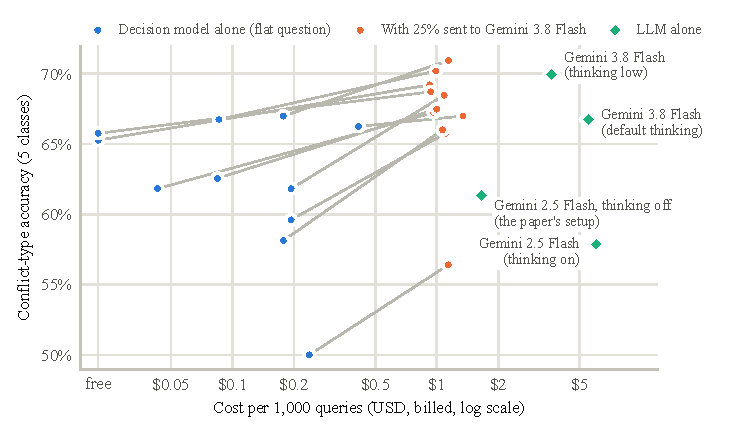
\includegraphics[width=0.78\textwidth]{figures/cascade_cost_accuracy.pdf}
\caption{Accuracy against cost (log scale) on the test split. Curves: \jev answers first and the least confident
fraction of queries goes to Gemini~3.8 Flash; dots mark 25\% and 50\% escalated (at 25\% the two curves nearly
coincide). Diamonds: LLMs alone with the paper's prompt.}
\label{fig:cascade}
\end{figure*}

\subsection{Diagnostics}
\label{sec:diagnostics}

We specified three hypotheses and their tests before running them; Tables~\ref{tab:diagnostics}
and~\ref{tab:plant} give the results. An identical rerun sets the noise floor: no system is deterministic, and
\jev changes its predicted type on \diagjfrerunflip\% of queries with nothing changed (Gemini~3.8 Flash:
\diaggmrerunflip\%).

\input{generated/tab_diagnostics}

\paragraph{Dates do not matter.} \jev's documentation lists ordering dates as a known weakness
\citep{typesafe2026jagged}, and we expected it to explain errors on \emph{Outdated}. It does not. Removing every
date changes no system's accuracy beyond the noise floor (\jev: \diagjfnodatesdiff points, $p\diagjfnodatesp$;
Gemini: \diaggmnodatesdiff, $p\diaggmnodatesp$), and neither does adding each result's recency rank computed in
code. \jev's recall on \emph{Outdated} is \diagjforigrec\% originally, \diagjfnodatesrec\% without dates and
\diagjfdatesincoderec\% with code-computed recency, at or above Gemini's in every condition. The systems recognise
outdated sources from their content (phrases such as ``former'' or ``as of'', and conflicting values), not from
publication dates. The weak \emph{Outdated} score of tree v2 comes from its question design, not from dates.

\paragraph{Order sensitivity is real but not specific to \jev.} Shuffling the results changes \jev's predicted type
on \diagjfshuffleflip\% of queries [\diagjfshufflelo, \diagjfshufflehi] over both seeds, well above its
\diagjfrerunflip\% noise floor; Gemini~3.8 Flash flips on \diaggmshuffleflip\%
[\diaggmshufflelo, \diaggmshufflehi]. On the same shuffles the two do not differ ($p\diagflipjevvsgonep$ and $p\diagflipjevvsgtwop$). Accuracy moves by at most a few points in either direction.

\input{generated/tab_plant}

\paragraph{A planted false source is noticed as well as by the LLM.} \conflicts has too few \emph{Misinformation}
queries to evaluate. We construct them: in \nplant \emph{No conflict} test queries whose gold answer appears in some
result, we rewrite one such result so that it states a plausible wrong answer, produced by a third model
(GPT-4.1-mini) so that neither classifier judges its own text. The expected label becomes \emph{Misinformation}.
Flat \jev labels \plantjfhit\% of planted queries as misinformation against \plantgmhit\% for Gemini~3.8 Flash
($p\planthitp$), but it also does so for \plantjffa\% of the clean versions of the same queries against
\plantgmfa\% ($p\plantfap$). Net of false alarms the two are identical (Youden \plantjfyouden each; difference
\plantyoudendiff [\plantyoudenlo, \plantyoudenhi]). \jev's misinformation probability separates planted from clean
versions with AUROC \plantjfauroc, so a threshold can trade detections for fewer false alarms. Tree v2, whose
misinformation rule was chosen on a development split with a single misinformation query, detects only
\plantjthit\%.

\subsection{Robustness across versions and decision models}
\label{sec:robustness}

\paragraph{\jev 1.14.} The newer version behaves like 1.13 (Table~\ref{tab:main}): \onefouracc\% with the flat
question (\onefourvsonethreediff points, $p\onefourvsonethreep$) and \onefourtreeacc\% with tree v2
($p\onefourtreevsonethreep$), still tied with Gemini~2.5 Flash ($p\onefourvstwofivep$), with the same failure
of tree v1 and the same cascade behaviour (tree v2 at 50\%: \onefourcascfiftyacc\%, $p\onefourcascfiftyp$ against
the LLM alone).

\input{generated/tab_decision_models}

\paragraph{Other decision models.} Table~\ref{tab:decision_models} places \jev among the decision models
available through the same gateway. \jev is mid-pack in accuracy and the fastest. Perplexity's decider is the most
accurate: \pplxflatacc\% with the flat question, \pplxvsjevdiffabs points above \jev ($p\pplxvsjevp$), and
\pplxtreeacc\% with tree v2, statistically tied with Gemini~3.8 Flash ($p\pplxtreevsgp$). As a cascade first
stage it reaches \cascpplxtfacc\% at \cascpplxtfcost\% of the LLM's cost at $f=25\%$. Not every decision model's
confidence is useful for escalation: GPT-6-luna's confidence barely ranks its errors (AUROC \lunaauroc), and its
25\% cascade is no better than random escalation (\lunacasctf\% vs.\ \lunacasctfrand\%).

\section{Discussion}
\label{sec:discussion}

\paragraph{What decision models offer as conflict classifiers.} Conflict typing sits on the critical path of every
search-augmented answer, so its latency and cost add to every request. Most hosted decision models classify a query
with about ten retrieved pages in under half a second, for at most \$\dmcostmax per thousand queries, with the accuracy of the LLM used in the original study. When the accuracy of a
current LLM is required, a decision model's confidence is usually good enough to route only its uncertain queries to
the LLM, which recovers most of the gap at a quarter to a third of the LLM's cost. End to end, the cheaper types cost
no measurable answer quality (\S\ref{sec:endtoend}). 

\paragraph{Choosing among decision models.} The class is not uniform. Accuracy spans \dmaccmin--\dmaccmax\%, and the
model at the bottom is significantly worse than the paper's LLM. Two properties that matter in deployment vary
independently of accuracy: calibration (ECE \eceminimum--\ecemaximum) and how well confidence ranks errors, which
decides whether a cascade helps at all. One of the most accurate models has confidence that is no better than random for
escalation. A model for this task should therefore be chosen on all three, measured on the deployment's own data,
not on accuracy alone.

\paragraph{How to ask.} The direct choice question was the reliable format for every model. The yes/no
decomposition looked natural but failed for all of them; the repaired tree encodes choices fitted to one model on a
small development split and did not help any other. For a new decision model we would start from the flat
question.

\paragraph{What the diagnostics change.} Dates turned out not to matter: outdated sources are recognised
from their content. Sensitivity to source order is real but differs so much between models that it has to be
measured for each one. A single false source is the subtle case, visible in the probabilities but rarely in the
top label. With
\nmisitest natural \emph{Misinformation} test queries, that type is the one a deployment would most need to
calibrate on its own data.

\paragraph{Limitations.}
(i) \conflicts is small: with \ntest test queries, differences under about five points are not significant, and the
cascades can be shown close to, but not formally equivalent to, the LLM. (ii) The label distribution reflects how the
queries were selected, not real search traffic, and the dataset has only five natural \emph{Misinformation}
queries; our planted variant tests one kind of misinformation (an entity or value substituted in a single source).
(iii) The census covers the decision models one gateway served on one day. Hosted models change without notice:
several identifiers are unversioned, two models were free during our runs, and our rerun of Gemini~2.5 Flash scores
below the published figure. Providers
do not disclose model sizes or training data, so we cannot explain the differences between models. (iv) The end-to-end test uses one generator and LLM judges, validated on \nvalid answers, that do not see the
search results; as in the original study, the primary judge is the generator's own model, which may favour its
answers \citep{panickssery2024llm}. The size of the gain from predicted types depends on the judge, and we do not
measure factual grounding, the third metric of \citet{cattan2025dragged}. (v) Not every system is deterministic: identical requests changed
up to \rerunflipmax\% of a decision model's predictions, and \diaggmrerunflip\% of Gemini~3.8 Flash's.

\section{Conclusion}
\label{sec:conclusion}

We tested every typed decision model hosted on one gateway as a classifier of knowledge-conflict types, using
the benchmark authors' protocol and the same inputs as the LLMs. Most match the LLM of the original study. They do
so at a small fraction of its cost and latency. They trail the
current LLM, but for most of them a confidence-gated cascade recovers that gap at a quarter to a third of the LLM's
cost, and given to a generator, their types yield answers that follow the expected behaviour as often as the LLM's.
 Future work should measure the gain from predicted types with judges that see the
sources, and test whether a decision model's probabilities can steer a generator between expected behaviours when
the type is uncertain.

\section*{Ethics and Broader Impact}

The planted-misinformation variant rewrites one retrieved page per query to state a wrong answer. It uses public data and factual substitutions on
non-sensitive questions, and is released with clear labels. All queries in \conflicts are safe by construction \citep{cattan2025dragged}. Cheap conflict
classification could be misused to suppress minority viewpoints; the expected behaviour for \emph{Conflicting
opinions} is to present all of them.


\bibliography{refs}
\bibliographystyle{acl_natbib}

\appendix
\section{Prompts and Questions}
\label{app:prompts}

\paragraph{LLM prompt.} The conflict-type prompt of \citet{cattan2025dragged}, copied from the paper's source with
only the \LaTeX{} bold markers removed. \texttt{\{search\_results\}} is filled with the numbered results.

\lstinputlisting{generated/paper_prompt.txt}

\paragraph{\jev, flat.} One choice question. Its instruction is the first paragraph of the prompt above; its options
are the five category definitions with their examples, word for word.

\lstinputlisting{generated/flat_question.txt}

\paragraph{\jev, tree.} Five yes/no questions asked in one request over the same state.

\lstinputlisting{generated/tree_questions.txt}

\paragraph{Planted wrong answers.} Prompt sent to GPT-4.1-mini (temperature 0) to obtain a plausible wrong answer
for each \emph{No conflict} query whose gold answer appears in a result. The answer is then replaced, as whole words
and case-insensitively, in the title, snippet and text of one such result chosen with a fixed seed. Queries whose
gold answer is \emph{yes} or \emph{no} are excluded.

\lstinputlisting{generated/wrong_answer_prompt.txt}

\section{Protocol Record}
\label{app:protocol}

The development/test split, the prompt and question texts and the combination rules were frozen with recorded file
hashes before any test-set call. Changes after that point were limited to the following, each logged with its reason
before results were computed: (1) Gemini~2.5 Flash with thinking added as a sensitivity check; (2) the answer parser
made lenient for category statements outside the requested JSON, applied to stored answers without new calls (no
strictly formatted answer changed); (3) Gemini~3.8 Flash added at two thinking levels; (4) the cascade, its
operating points and its controls; (5) the diagnostics, with one amendment before any planted run: whole-word
matching and the exclusion of yes/no answers, after substring matching was found to alter unrelated numbers;
(6) \jev 1.14 and the four other decision models, run with \jev's frozen questions. All runs were reported. Code,
splits, prompts, cached responses and per-query outputs are released.


\end{document}
"
%   arXiv preprint:        scripts/make_arxiv.sh  (authors shown, no line numbers or header)
\ifdefined\taclfinal\def\taclauthors{}\fi
\ifdefined\arxivversion\def\taclauthors{}\fi
\ifdefined\taclauthors\usepackage[acceptedWithA]{tacl2021v1}\else\usepackage{tacl2021v1}\fi
% The author block needs more than the style's default 5 cm title box (its own advice: set \titlebox right
% after loading the style). Not needed for the anonymous submission.
\ifdefined\taclauthors\setlength\titlebox{6.5cm}\fi
% PDF metadata: title always; authors only in the builds that show them.
\hypersetup{pdftitle={Do We Need an LLM to Know Why Sources Conflict? Decision Models for Knowledge-Conflict Typing in RAG}}
\ifdefined\taclauthors\hypersetup{pdfauthor={Parv Khatri, Harshul Jain, Mehak Kapoor, Tanya Sah}}\fi
% Code release: linked only in the versions that show authors (arXiv, camera-ready). The anonymous
% TACL submission may not link to code, so it only says that everything is released.
\newcommand{\repourl}{https://github.com/Parv17k/decision-models-conflict-typing}
\ifdefined\taclauthors\newcommand{\releasenote}{ at \url{\repourl}}\else\newcommand{\releasenote}{}\fi
\usepackage{xspace}
\xspaceaddexceptions{\% $ ] ) / , ;}   % no space between a generated number and %, $, brackets or punctuation
\usepackage{booktabs}
\usepackage{graphicx}
\usepackage{amsmath}
\usepackage{xcolor}
\usepackage{tikz}
\usepackage{listings}

\lstset{basicstyle=\scriptsize\ttfamily,breaklines=true,breakatwhitespace=true,columns=fullflexible,
        frame=single,framerule=0.4pt,rulecolor=\color{gray},xleftmargin=2pt,xrightmargin=2pt}
% Shrink a table to the line width only if it is wider (graphicx only; no adjustbox in BasicTeX).
\newsavebox{\fitbox}
\newcommand{\fitwidth}[1]{\sbox{\fitbox}{#1}\ifdim\wd\fitbox>\linewidth\typeout{FITWIDTH scaled \the\wd\fitbox\space to \the\linewidth}\resizebox{\linewidth}{!}{\usebox{\fitbox}}\else\usebox{\fitbox}\fi}
% References ragged-right: in a justified narrow column, long URLs otherwise stretch with visible gaps.
\makeatletter\let\dm@thebibliography\thebibliography
\renewcommand{\thebibliography}[1]{\dm@thebibliography{#1}\raggedright}\makeatother
\newcommand{\todo}[1]{\textcolor{orange!80!black}{[TODO: #1]}}
\newcommand{\jev}{Jev\xspace}
\newcommand{\conflicts}{\textsc{Conflicts}\xspace}

% Generated by scripts/make_tables.py from the stored runs. Do not edit.
\newcommand{\allgtwofive}{60.7\xspace}
\newcommand{\aurocmax}{0.76\xspace}
\newcommand{\aurocmin}{0.64\xspace}
\newcommand{\avgresults}{9.2\xspace}
\newcommand{\cascelephantfiftyacc}{70.0\xspace}
\newcommand{\cascelephantfiftycost}{50\xspace}
\newcommand{\cascelephantfiftydiff}{+0.0\xspace}
\newcommand{\cascelephantfiftydiffabs}{0.0\xspace}
\newcommand{\cascelephantfiftyhi}{+2.0\xspace}
\newcommand{\cascelephantfiftyhiabs}{2.0\xspace}
\newcommand{\cascelephantfiftylat}{1.59\xspace}
\newcommand{\cascelephantfiftylo}{$-$2.0\xspace}
\newcommand{\cascelephantfiftyloabs}{2.0\xspace}
\newcommand{\cascelephantfiftyp}{=1.00\xspace}
\newcommand{\cascelephantfiftyrand}{67.6\xspace}
\newcommand{\cascelephanttfacc}{69.2\xspace}
\newcommand{\cascelephanttfcost}{25\xspace}
\newcommand{\cascelephanttfdiff}{$-$0.7\xspace}
\newcommand{\cascelephanttfdiffabs}{0.7\xspace}
\newcommand{\cascelephanttfhi}{+2.5\xspace}
\newcommand{\cascelephanttfhiabs}{2.5\xspace}
\newcommand{\cascelephanttflat}{1.02\xspace}
\newcommand{\cascelephanttflo}{$-$3.9\xspace}
\newcommand{\cascelephanttfloabs}{3.9\xspace}
\newcommand{\cascelephanttfp}{=0.77\xspace}
\newcommand{\cascelephanttfrand}{66.4\xspace}
\newcommand{\cascgainmax}{4.9\xspace}
\newcommand{\cascgainmin}{-0.2\xspace}
\newcommand{\cascjevfiftyacc}{69.2\xspace}
\newcommand{\cascjevfiftycost}{54\xspace}
\newcommand{\cascjevfiftydiff}{$-$0.7\xspace}
\newcommand{\cascjevfiftydiffabs}{0.7\xspace}
\newcommand{\cascjevfiftyhi}{+1.0\xspace}
\newcommand{\cascjevfiftyhiabs}{1.0\xspace}
\newcommand{\cascjevfiftylat}{1.34\xspace}
\newcommand{\cascjevfiftylo}{$-$2.7\xspace}
\newcommand{\cascjevfiftyloabs}{2.7\xspace}
\newcommand{\cascjevfiftyp}{=0.61\xspace}
\newcommand{\cascjevfiftyrand}{65.9\xspace}
\newcommand{\cascjevnewfiftyacc}{68.7\xspace}
\newcommand{\cascjevnewfiftycost}{54\xspace}
\newcommand{\cascjevnewfiftydiff}{$-$1.2\xspace}
\newcommand{\cascjevnewfiftydiffabs}{1.2\xspace}
\newcommand{\cascjevnewfiftyhi}{+1.0\xspace}
\newcommand{\cascjevnewfiftyhiabs}{1.0\xspace}
\newcommand{\cascjevnewfiftylat}{1.36\xspace}
\newcommand{\cascjevnewfiftylo}{$-$3.4\xspace}
\newcommand{\cascjevnewfiftyloabs}{3.4\xspace}
\newcommand{\cascjevnewfiftyp}{=0.36\xspace}
\newcommand{\cascjevnewfiftyrand}{64.8\xspace}
\newcommand{\cascjevnewtfacc}{65.8\xspace}
\newcommand{\cascjevnewtfcost}{30\xspace}
\newcommand{\cascjevnewtfdiff}{$-$4.2\xspace}
\newcommand{\cascjevnewtfdiffabs}{4.2\xspace}
\newcommand{\cascjevnewtfhi}{$-$1.0\xspace}
\newcommand{\cascjevnewtfhiabs}{1.0\xspace}
\newcommand{\cascjevnewtflat}{0.82\xspace}
\newcommand{\cascjevnewtflo}{$-$7.4\xspace}
\newcommand{\cascjevnewtfloabs}{7.4\xspace}
\newcommand{\cascjevnewtfp}{=0.016\xspace}
\newcommand{\cascjevnewtfrand}{62.2\xspace}
\newcommand{\cascjevtfacc}{68.5\xspace}
\newcommand{\cascjevtfcost}{30\xspace}
\newcommand{\cascjevtfdiff}{$-$1.5\xspace}
\newcommand{\cascjevtfdiffabs}{1.5\xspace}
\newcommand{\cascjevtfhi}{+1.5\xspace}
\newcommand{\cascjevtfhiabs}{1.5\xspace}
\newcommand{\cascjevtflat}{0.81\xspace}
\newcommand{\cascjevtflo}{$-$4.4\xspace}
\newcommand{\cascjevtfloabs}{4.4\xspace}
\newcommand{\cascjevtfp}{=0.41\xspace}
\newcommand{\cascjevtfrand}{63.9\xspace}
\newcommand{\cascliquidfiftyacc}{69.2\xspace}
\newcommand{\cascliquidfiftycost}{52\xspace}
\newcommand{\cascliquidfiftydiff}{$-$0.7\xspace}
\newcommand{\cascliquidfiftydiffabs}{0.7\xspace}
\newcommand{\cascliquidfiftyhi}{+0.7\xspace}
\newcommand{\cascliquidfiftyhiabs}{0.7\xspace}
\newcommand{\cascliquidfiftylat}{1.51\xspace}
\newcommand{\cascliquidfiftylo}{$-$2.5\xspace}
\newcommand{\cascliquidfiftyloabs}{2.5\xspace}
\newcommand{\cascliquidfiftyp}{=0.55\xspace}
\newcommand{\cascliquidfiftyrand}{66.3\xspace}
\newcommand{\cascliquidtfacc}{67.5\xspace}
\newcommand{\cascliquidtfcost}{27\xspace}
\newcommand{\cascliquidtfdiff}{$-$2.5\xspace}
\newcommand{\cascliquidtfdiffabs}{2.5\xspace}
\newcommand{\cascliquidtfhi}{+0.5\xspace}
\newcommand{\cascliquidtfhiabs}{0.5\xspace}
\newcommand{\cascliquidtflat}{0.97\xspace}
\newcommand{\cascliquidtflo}{$-$5.4\xspace}
\newcommand{\cascliquidtfloabs}{5.4\xspace}
\newcommand{\cascliquidtfp}{=0.14\xspace}
\newcommand{\cascliquidtfrand}{64.4\xspace}
\newcommand{\cascliquidultrafiftyacc}{70.4\xspace}
\newcommand{\cascliquidultrafiftycost}{55\xspace}
\newcommand{\cascliquidultrafiftydiff}{+0.5\xspace}
\newcommand{\cascliquidultrafiftydiffabs}{0.5\xspace}
\newcommand{\cascliquidultrafiftyhi}{+2.2\xspace}
\newcommand{\cascliquidultrafiftyhiabs}{2.2\xspace}
\newcommand{\cascliquidultrafiftylat}{1.59\xspace}
\newcommand{\cascliquidultrafiftylo}{$-$1.2\xspace}
\newcommand{\cascliquidultrafiftyloabs}{1.2\xspace}
\newcommand{\cascliquidultrafiftyp}{=0.77\xspace}
\newcommand{\cascliquidultrafiftyrand}{68.5\xspace}
\newcommand{\cascliquidultratfacc}{70.9\xspace}
\newcommand{\cascliquidultratfcost}{31\xspace}
\newcommand{\cascliquidultratfdiff}{+1.0\xspace}
\newcommand{\cascliquidultratfdiffabs}{1.0\xspace}
\newcommand{\cascliquidultratfhi}{+3.9\xspace}
\newcommand{\cascliquidultratfhiabs}{3.9\xspace}
\newcommand{\cascliquidultratflat}{1.05\xspace}
\newcommand{\cascliquidultratflo}{$-$2.0\xspace}
\newcommand{\cascliquidultratfloabs}{2.0\xspace}
\newcommand{\cascliquidultratfp}{=0.63\xspace}
\newcommand{\cascliquidultratfrand}{67.7\xspace}
\newcommand{\casclunafiftyacc}{69.0\xspace}
\newcommand{\casclunafiftycost}{61\xspace}
\newcommand{\casclunafiftydiff}{$-$1.0\xspace}
\newcommand{\casclunafiftydiffabs}{1.0\xspace}
\newcommand{\casclunafiftyhi}{+1.0\xspace}
\newcommand{\casclunafiftyhiabs}{1.0\xspace}
\newcommand{\casclunafiftylat}{1.42\xspace}
\newcommand{\casclunafiftylo}{$-$3.0\xspace}
\newcommand{\casclunafiftyloabs}{3.0\xspace}
\newcommand{\casclunafiftyp}{=0.48\xspace}
\newcommand{\casclunafiftyrand}{68.1\xspace}
\newcommand{\casclunatfacc}{67.0\xspace}
\newcommand{\casclunatfcost}{37\xspace}
\newcommand{\casclunatfdiff}{$-$3.0\xspace}
\newcommand{\casclunatfdiffabs}{3.0\xspace}
\newcommand{\casclunatfhi}{+0.2\xspace}
\newcommand{\casclunatfhiabs}{0.2\xspace}
\newcommand{\casclunatflat}{0.89\xspace}
\newcommand{\casclunatflo}{$-$6.2\xspace}
\newcommand{\casclunatfloabs}{6.2\xspace}
\newcommand{\casclunatfp}{=0.10\xspace}
\newcommand{\casclunatfrand}{67.2\xspace}
\newcommand{\cascmammothfiftyacc}{70.2\xspace}
\newcommand{\cascmammothfiftycost}{50\xspace}
\newcommand{\cascmammothfiftydiff}{+0.2\xspace}
\newcommand{\cascmammothfiftydiffabs}{0.2\xspace}
\newcommand{\cascmammothfiftyhi}{+1.7\xspace}
\newcommand{\cascmammothfiftyhiabs}{1.7\xspace}
\newcommand{\cascmammothfiftylat}{1.71\xspace}
\newcommand{\cascmammothfiftylo}{$-$1.2\xspace}
\newcommand{\cascmammothfiftyloabs}{1.2\xspace}
\newcommand{\cascmammothfiftyp}{=1.00\xspace}
\newcommand{\cascmammothfiftyrand}{67.9\xspace}
\newcommand{\cascmammothtfacc}{68.7\xspace}
\newcommand{\cascmammothtfcost}{26\xspace}
\newcommand{\cascmammothtfdiff}{$-$1.2\xspace}
\newcommand{\cascmammothtfdiffabs}{1.2\xspace}
\newcommand{\cascmammothtfhi}{+1.5\xspace}
\newcommand{\cascmammothtfhiabs}{1.5\xspace}
\newcommand{\cascmammothtflat}{1.18\xspace}
\newcommand{\cascmammothtflo}{$-$3.9\xspace}
\newcommand{\cascmammothtfloabs}{3.9\xspace}
\newcommand{\cascmammothtfp}{=0.49\xspace}
\newcommand{\cascmammothtfrand}{66.8\xspace}
\newcommand{\cascmsftfiftyacc}{69.2\xspace}
\newcommand{\cascmsftfiftycost}{54\xspace}
\newcommand{\cascmsftfiftydiff}{$-$0.7\xspace}
\newcommand{\cascmsftfiftydiffabs}{0.7\xspace}
\newcommand{\cascmsftfiftyhi}{+1.2\xspace}
\newcommand{\cascmsftfiftyhiabs}{1.2\xspace}
\newcommand{\cascmsftfiftylat}{1.54\xspace}
\newcommand{\cascmsftfiftylo}{$-$3.0\xspace}
\newcommand{\cascmsftfiftyloabs}{3.0\xspace}
\newcommand{\cascmsftfiftyp}{=0.65\xspace}
\newcommand{\cascmsftfiftyrand}{64.0\xspace}
\newcommand{\cascmsfttfacc}{66.0\xspace}
\newcommand{\cascmsfttfcost}{29\xspace}
\newcommand{\cascmsfttfdiff}{$-$3.9\xspace}
\newcommand{\cascmsfttfdiffabs}{3.9\xspace}
\newcommand{\cascmsfttfhi}{$-$0.5\xspace}
\newcommand{\cascmsfttfhiabs}{0.5\xspace}
\newcommand{\cascmsfttflat}{0.97\xspace}
\newcommand{\cascmsfttflo}{$-$7.6\xspace}
\newcommand{\cascmsfttfloabs}{7.6\xspace}
\newcommand{\cascmsfttfp}{=0.048\xspace}
\newcommand{\cascmsfttfrand}{61.1\xspace}
\newcommand{\cascpplxfiftyacc}{70.0\xspace}
\newcommand{\cascpplxfiftycost}{52\xspace}
\newcommand{\cascpplxfiftydiff}{+0.0\xspace}
\newcommand{\cascpplxfiftydiffabs}{0.0\xspace}
\newcommand{\cascpplxfiftyhi}{+1.5\xspace}
\newcommand{\cascpplxfiftyhiabs}{1.5\xspace}
\newcommand{\cascpplxfiftylat}{1.54\xspace}
\newcommand{\cascpplxfiftylo}{$-$1.5\xspace}
\newcommand{\cascpplxfiftyloabs}{1.5\xspace}
\newcommand{\cascpplxfiftyp}{=1.00\xspace}
\newcommand{\cascpplxfiftyrand}{68.3\xspace}
\newcommand{\cascpplxflashfiftyacc}{68.5\xspace}
\newcommand{\cascpplxflashfiftycost}{51\xspace}
\newcommand{\cascpplxflashfiftydiff}{$-$1.5\xspace}
\newcommand{\cascpplxflashfiftydiffabs}{1.5\xspace}
\newcommand{\cascpplxflashfiftyhi}{+0.7\xspace}
\newcommand{\cascpplxflashfiftyhiabs}{0.7\xspace}
\newcommand{\cascpplxflashfiftylat}{1.43\xspace}
\newcommand{\cascpplxflashfiftylo}{$-$3.7\xspace}
\newcommand{\cascpplxflashfiftyloabs}{3.7\xspace}
\newcommand{\cascpplxflashfiftyp}{=0.26\xspace}
\newcommand{\cascpplxflashfiftyrand}{65.9\xspace}
\newcommand{\cascpplxflashtfacc}{67.2\xspace}
\newcommand{\cascpplxflashtfcost}{26\xspace}
\newcommand{\cascpplxflashtfdiff}{$-$2.7\xspace}
\newcommand{\cascpplxflashtfdiffabs}{2.7\xspace}
\newcommand{\cascpplxflashtfhi}{+0.2\xspace}
\newcommand{\cascpplxflashtfhiabs}{0.2\xspace}
\newcommand{\cascpplxflashtflat}{0.87\xspace}
\newcommand{\cascpplxflashtflo}{$-$5.9\xspace}
\newcommand{\cascpplxflashtfloabs}{5.9\xspace}
\newcommand{\cascpplxflashtfp}{=0.13\xspace}
\newcommand{\cascpplxflashtfrand}{63.9\xspace}
\newcommand{\cascpplxtfacc}{70.2\xspace}
\newcommand{\cascpplxtfcost}{27\xspace}
\newcommand{\cascpplxtfdiff}{+0.2\xspace}
\newcommand{\cascpplxtfdiffabs}{0.2\xspace}
\newcommand{\cascpplxtfhi}{+2.7\xspace}
\newcommand{\cascpplxtfhiabs}{2.7\xspace}
\newcommand{\cascpplxtflat}{0.97\xspace}
\newcommand{\cascpplxtflo}{$-$2.2\xspace}
\newcommand{\cascpplxtfloabs}{2.2\xspace}
\newcommand{\cascpplxtfp}{=1.00\xspace}
\newcommand{\cascpplxtfrand}{67.6\xspace}
\newcommand{\cascscaledownfiftyacc}{62.8\xspace}
\newcommand{\cascscaledownfiftycost}{57\xspace}
\newcommand{\cascscaledownfiftydiff}{$-$7.1\xspace}
\newcommand{\cascscaledownfiftydiffabs}{7.1\xspace}
\newcommand{\cascscaledownfiftyhi}{$-$3.7\xspace}
\newcommand{\cascscaledownfiftyhiabs}{3.7\xspace}
\newcommand{\cascscaledownfiftylat}{1.83\xspace}
\newcommand{\cascscaledownfiftylo}{$-$10.8\xspace}
\newcommand{\cascscaledownfiftyloabs}{10.8\xspace}
\newcommand{\cascscaledownfiftyp}{<0.001\xspace}
\newcommand{\cascscaledownfiftyrand}{60.0\xspace}
\newcommand{\cascscaledowntfacc}{56.4\xspace}
\newcommand{\cascscaledowntfcost}{31\xspace}
\newcommand{\cascscaledowntfdiff}{$-$13.5\xspace}
\newcommand{\cascscaledowntfdiffabs}{13.5\xspace}
\newcommand{\cascscaledowntfhi}{$-$8.9\xspace}
\newcommand{\cascscaledowntfhiabs}{8.9\xspace}
\newcommand{\cascscaledowntflat}{1.29\xspace}
\newcommand{\cascscaledowntflo}{$-$18.0\xspace}
\newcommand{\cascscaledowntfloabs}{18.0\xspace}
\newcommand{\cascscaledowntfp}{<0.001\xspace}
\newcommand{\cascscaledowntfrand}{55.0\xspace}
\newcommand{\casctiedcostmax}{37\xspace}
\newcommand{\casctiedcostmin}{25\xspace}
\newcommand{\cihalf}{4.8\xspace}
\newcommand{\costratiorefmax}{39\xspace}
\newcommand{\costratiorefmin}{4\xspace}
\newcommand{\costratiorefnow}{2.2\xspace}
\newcommand{\devcompatcomp}{0.81\xspace}
\newcommand{\devcompatopin}{0.69\xspace}
\newcommand{\devmisinfohi}{0.79\xspace}
\newcommand{\devmisinfolo}{0.53\xspace}
\newcommand{\devnopin}{13\xspace}
\newcommand{\devopinionauroc}{0.83\xspace}
\newcommand{\devopintocomp}{12\xspace}
\newcommand{\diagelephantdatesincodediff}{+0.7\xspace}
\newcommand{\diagelephantdatesincodediffabs}{0.7\xspace}
\newcommand{\diagelephantdatesincodehi}{+2.5\xspace}
\newcommand{\diagelephantdatesincodehiabs}{2.5\xspace}
\newcommand{\diagelephantdatesincodelo}{$-$0.7\xspace}
\newcommand{\diagelephantdatesincodeloabs}{0.7\xspace}
\newcommand{\diagelephantdatesincodep}{=0.55\xspace}
\newcommand{\diagelephantdatesincoderec}{58.2\xspace}
\newcommand{\diagelephantnodatesdiff}{+0.5\xspace}
\newcommand{\diagelephantnodatesdiffabs}{0.5\xspace}
\newcommand{\diagelephantnodateshi}{+2.5\xspace}
\newcommand{\diagelephantnodateshiabs}{2.5\xspace}
\newcommand{\diagelephantnodateslo}{$-$1.5\xspace}
\newcommand{\diagelephantnodatesloabs}{1.5\xspace}
\newcommand{\diagelephantnodatesp}{=0.80\xspace}
\newcommand{\diagelephantnodatesrec}{65.5\xspace}
\newcommand{\diagelephantorigrec}{56.4\xspace}
\newcommand{\diagelephantrerunflip}{0.0\xspace}
\newcommand{\diagelephantshuffleflip}{7.3\xspace}
\newcommand{\diagelephantshufflehi}{9.1\xspace}
\newcommand{\diagelephantshufflelo}{5.5\xspace}
\newcommand{\diagelephantshuffleonediff}{$-$0.7\xspace}
\newcommand{\diagelephantshuffleonediffabs}{0.7\xspace}
\newcommand{\diagelephantshuffleonehi}{+1.5\xspace}
\newcommand{\diagelephantshuffleonehiabs}{1.5\xspace}
\newcommand{\diagelephantshuffleonelo}{$-$3.0\xspace}
\newcommand{\diagelephantshuffleoneloabs}{3.0\xspace}
\newcommand{\diagelephantshuffleonep}{=0.68\xspace}
\newcommand{\diagelephantshuffletwodiff}{$-$1.0\xspace}
\newcommand{\diagelephantshuffletwodiffabs}{1.0\xspace}
\newcommand{\diagelephantshuffletwohi}{+1.0\xspace}
\newcommand{\diagelephantshuffletwohiabs}{1.0\xspace}
\newcommand{\diagelephantshuffletwolo}{$-$3.0\xspace}
\newcommand{\diagelephantshuffletwoloabs}{3.0\xspace}
\newcommand{\diagelephantshuffletwop}{=0.48\xspace}
\newcommand{\diaggmdatesincodediff}{$-$0.7\xspace}
\newcommand{\diaggmdatesincodediffabs}{0.7\xspace}
\newcommand{\diaggmdatesincodehi}{+1.5\xspace}
\newcommand{\diaggmdatesincodehiabs}{1.5\xspace}
\newcommand{\diaggmdatesincodelo}{$-$2.7\xspace}
\newcommand{\diaggmdatesincodeloabs}{2.7\xspace}
\newcommand{\diaggmdatesincodep}{=0.65\xspace}
\newcommand{\diaggmdatesincoderec}{72.7\xspace}
\newcommand{\diaggmnodatesdiff}{$-$0.7\xspace}
\newcommand{\diaggmnodatesdiffabs}{0.7\xspace}
\newcommand{\diaggmnodateshi}{+0.7\xspace}
\newcommand{\diaggmnodateshiabs}{0.7\xspace}
\newcommand{\diaggmnodateslo}{$-$2.2\xspace}
\newcommand{\diaggmnodatesloabs}{2.2\xspace}
\newcommand{\diaggmnodatesp}{=0.51\xspace}
\newcommand{\diaggmnodatesrec}{67.3\xspace}
\newcommand{\diaggmorigrec}{69.1\xspace}
\newcommand{\diaggmrerunflip}{3.4\xspace}
\newcommand{\diaggmshuffleflip}{9.4\xspace}
\newcommand{\diaggmshufflehi}{11.5\xspace}
\newcommand{\diaggmshufflelo}{7.5\xspace}
\newcommand{\diagjevdatesincodediff}{+0.2\xspace}
\newcommand{\diagjevdatesincodediffabs}{0.2\xspace}
\newcommand{\diagjevdatesincodehi}{+1.7\xspace}
\newcommand{\diagjevdatesincodehiabs}{1.7\xspace}
\newcommand{\diagjevdatesincodelo}{$-$1.2\xspace}
\newcommand{\diagjevdatesincodeloabs}{1.2\xspace}
\newcommand{\diagjevdatesincodep}{=1.00\xspace}
\newcommand{\diagjevdatesincoderec}{76.4\xspace}
\newcommand{\diagjevnewdatesincodediff}{+1.0\xspace}
\newcommand{\diagjevnewdatesincodediffabs}{1.0\xspace}
\newcommand{\diagjevnewdatesincodehi}{+2.7\xspace}
\newcommand{\diagjevnewdatesincodehiabs}{2.7\xspace}
\newcommand{\diagjevnewdatesincodelo}{$-$0.7\xspace}
\newcommand{\diagjevnewdatesincodeloabs}{0.7\xspace}
\newcommand{\diagjevnewdatesincodep}{=0.39\xspace}
\newcommand{\diagjevnewdatesincoderec}{80.0\xspace}
\newcommand{\diagjevnewnodatesdiff}{+0.0\xspace}
\newcommand{\diagjevnewnodatesdiffabs}{0.0\xspace}
\newcommand{\diagjevnewnodateshi}{+1.2\xspace}
\newcommand{\diagjevnewnodateshiabs}{1.2\xspace}
\newcommand{\diagjevnewnodateslo}{$-$1.2\xspace}
\newcommand{\diagjevnewnodatesloabs}{1.2\xspace}
\newcommand{\diagjevnewnodatesp}{=1.00\xspace}
\newcommand{\diagjevnewnodatesrec}{76.4\xspace}
\newcommand{\diagjevneworigrec}{76.4\xspace}
\newcommand{\diagjevnewrerunflip}{3.0\xspace}
\newcommand{\diagjevnewshuffleflip}{10.8\xspace}
\newcommand{\diagjevnewshufflehi}{12.9\xspace}
\newcommand{\diagjevnewshufflelo}{8.7\xspace}
\newcommand{\diagjevnewshuffleonediff}{+1.0\xspace}
\newcommand{\diagjevnewshuffleonediffabs}{1.0\xspace}
\newcommand{\diagjevnewshuffleonehi}{+3.7\xspace}
\newcommand{\diagjevnewshuffleonehiabs}{3.7\xspace}
\newcommand{\diagjevnewshuffleonelo}{$-$1.7\xspace}
\newcommand{\diagjevnewshuffleoneloabs}{1.7\xspace}
\newcommand{\diagjevnewshuffleonep}{=0.60\xspace}
\newcommand{\diagjevnewshuffletwodiff}{+0.0\xspace}
\newcommand{\diagjevnewshuffletwodiffabs}{0.0\xspace}
\newcommand{\diagjevnewshuffletwohi}{+2.5\xspace}
\newcommand{\diagjevnewshuffletwohiabs}{2.5\xspace}
\newcommand{\diagjevnewshuffletwolo}{$-$2.5\xspace}
\newcommand{\diagjevnewshuffletwoloabs}{2.5\xspace}
\newcommand{\diagjevnewshuffletwop}{=1.00\xspace}
\newcommand{\diagjevnodatesdiff}{$-$1.0\xspace}
\newcommand{\diagjevnodatesdiffabs}{1.0\xspace}
\newcommand{\diagjevnodateshi}{+0.5\xspace}
\newcommand{\diagjevnodateshiabs}{0.5\xspace}
\newcommand{\diagjevnodateslo}{$-$2.5\xspace}
\newcommand{\diagjevnodatesloabs}{2.5\xspace}
\newcommand{\diagjevnodatesp}{=0.34\xspace}
\newcommand{\diagjevnodatesrec}{74.5\xspace}
\newcommand{\diagjevorigrec}{72.7\xspace}
\newcommand{\diagjevrerunflip}{2.0\xspace}
\newcommand{\diagjevshuffleflip}{11.6\xspace}
\newcommand{\diagjevshufflehi}{13.8\xspace}
\newcommand{\diagjevshufflelo}{9.4\xspace}
\newcommand{\diagjevshuffleonediff}{+1.5\xspace}
\newcommand{\diagjevshuffleonediffabs}{1.5\xspace}
\newcommand{\diagjevshuffleonehi}{+4.2\xspace}
\newcommand{\diagjevshuffleonehiabs}{4.2\xspace}
\newcommand{\diagjevshuffleonelo}{$-$1.2\xspace}
\newcommand{\diagjevshuffleoneloabs}{1.2\xspace}
\newcommand{\diagjevshuffleonep}{=0.38\xspace}
\newcommand{\diagjevshuffletwodiff}{+0.2\xspace}
\newcommand{\diagjevshuffletwodiffabs}{0.2\xspace}
\newcommand{\diagjevshuffletwohi}{+3.2\xspace}
\newcommand{\diagjevshuffletwohiabs}{3.2\xspace}
\newcommand{\diagjevshuffletwolo}{$-$2.7\xspace}
\newcommand{\diagjevshuffletwoloabs}{2.7\xspace}
\newcommand{\diagjevshuffletwop}{=1.00\xspace}
\newcommand{\diagliquiddatesincodediff}{$-$0.5\xspace}
\newcommand{\diagliquiddatesincodediffabs}{0.5\xspace}
\newcommand{\diagliquiddatesincodehi}{+1.7\xspace}
\newcommand{\diagliquiddatesincodehiabs}{1.7\xspace}
\newcommand{\diagliquiddatesincodelo}{$-$2.7\xspace}
\newcommand{\diagliquiddatesincodeloabs}{2.7\xspace}
\newcommand{\diagliquiddatesincodep}{=0.83\xspace}
\newcommand{\diagliquiddatesincoderec}{89.1\xspace}
\newcommand{\diagliquidnodatesdiff}{$-$0.2\xspace}
\newcommand{\diagliquidnodatesdiffabs}{0.2\xspace}
\newcommand{\diagliquidnodateshi}{+2.0\xspace}
\newcommand{\diagliquidnodateshiabs}{2.0\xspace}
\newcommand{\diagliquidnodateslo}{$-$2.5\xspace}
\newcommand{\diagliquidnodatesloabs}{2.5\xspace}
\newcommand{\diagliquidnodatesp}{=1.00\xspace}
\newcommand{\diagliquidnodatesrec}{81.8\xspace}
\newcommand{\diagliquidorigrec}{81.8\xspace}
\newcommand{\diagliquidrerunflip}{9.4\xspace}
\newcommand{\diagliquidshuffleflip}{15.5\xspace}
\newcommand{\diagliquidshufflehi}{18.0\xspace}
\newcommand{\diagliquidshufflelo}{13.1\xspace}
\newcommand{\diagliquidshuffleonediff}{+0.2\xspace}
\newcommand{\diagliquidshuffleonediffabs}{0.2\xspace}
\newcommand{\diagliquidshuffleonehi}{+3.7\xspace}
\newcommand{\diagliquidshuffleonehiabs}{3.7\xspace}
\newcommand{\diagliquidshuffleonelo}{$-$3.2\xspace}
\newcommand{\diagliquidshuffleoneloabs}{3.2\xspace}
\newcommand{\diagliquidshuffleonep}{=1.00\xspace}
\newcommand{\diagliquidshuffletwodiff}{+2.2\xspace}
\newcommand{\diagliquidshuffletwodiffabs}{2.2\xspace}
\newcommand{\diagliquidshuffletwohi}{+5.7\xspace}
\newcommand{\diagliquidshuffletwohiabs}{5.7\xspace}
\newcommand{\diagliquidshuffletwolo}{$-$1.2\xspace}
\newcommand{\diagliquidshuffletwoloabs}{1.2\xspace}
\newcommand{\diagliquidshuffletwop}{=0.25\xspace}
\newcommand{\diagliquidultradatesincodediff}{+0.0\xspace}
\newcommand{\diagliquidultradatesincodediffabs}{0.0\xspace}
\newcommand{\diagliquidultradatesincodehi}{+2.0\xspace}
\newcommand{\diagliquidultradatesincodehiabs}{2.0\xspace}
\newcommand{\diagliquidultradatesincodelo}{$-$1.7\xspace}
\newcommand{\diagliquidultradatesincodeloabs}{1.7\xspace}
\newcommand{\diagliquidultradatesincodep}{=1.00\xspace}
\newcommand{\diagliquidultradatesincoderec}{80.0\xspace}
\newcommand{\diagliquidultranodatesdiff}{+1.0\xspace}
\newcommand{\diagliquidultranodatesdiffabs}{1.0\xspace}
\newcommand{\diagliquidultranodateshi}{+3.0\xspace}
\newcommand{\diagliquidultranodateshiabs}{3.0\xspace}
\newcommand{\diagliquidultranodateslo}{$-$1.0\xspace}
\newcommand{\diagliquidultranodatesloabs}{1.0\xspace}
\newcommand{\diagliquidultranodatesp}{=0.45\xspace}
\newcommand{\diagliquidultranodatesrec}{78.2\xspace}
\newcommand{\diagliquidultraorigrec}{76.4\xspace}
\newcommand{\diagliquidultrarerunflip}{5.2\xspace}
\newcommand{\diagliquidultrashuffleflip}{7.4\xspace}
\newcommand{\diagliquidultrashufflehi}{9.2\xspace}
\newcommand{\diagliquidultrashufflelo}{5.7\xspace}
\newcommand{\diagliquidultrashuffleonediff}{+1.7\xspace}
\newcommand{\diagliquidultrashuffleonediffabs}{1.7\xspace}
\newcommand{\diagliquidultrashuffleonehi}{+4.2\xspace}
\newcommand{\diagliquidultrashuffleonehiabs}{4.2\xspace}
\newcommand{\diagliquidultrashuffleonelo}{$-$0.7\xspace}
\newcommand{\diagliquidultrashuffleoneloabs}{0.7\xspace}
\newcommand{\diagliquidultrashuffleonep}{=0.25\xspace}
\newcommand{\diagliquidultrashuffletwodiff}{+2.2\xspace}
\newcommand{\diagliquidultrashuffletwodiffabs}{2.2\xspace}
\newcommand{\diagliquidultrashuffletwohi}{+4.9\xspace}
\newcommand{\diagliquidultrashuffletwohiabs}{4.9\xspace}
\newcommand{\diagliquidultrashuffletwolo}{$-$0.2\xspace}
\newcommand{\diagliquidultrashuffletwoloabs}{0.2\xspace}
\newcommand{\diagliquidultrashuffletwop}{=0.12\xspace}
\newcommand{\diaglunadatesincodediff}{+0.0\xspace}
\newcommand{\diaglunadatesincodediffabs}{0.0\xspace}
\newcommand{\diaglunadatesincodehi}{+2.5\xspace}
\newcommand{\diaglunadatesincodehiabs}{2.5\xspace}
\newcommand{\diaglunadatesincodelo}{$-$2.5\xspace}
\newcommand{\diaglunadatesincodeloabs}{2.5\xspace}
\newcommand{\diaglunadatesincodep}{=1.00\xspace}
\newcommand{\diaglunadatesincoderec}{74.5\xspace}
\newcommand{\diaglunanodatesdiff}{$-$0.5\xspace}
\newcommand{\diaglunanodatesdiffabs}{0.5\xspace}
\newcommand{\diaglunanodateshi}{+2.0\xspace}
\newcommand{\diaglunanodateshiabs}{2.0\xspace}
\newcommand{\diaglunanodateslo}{$-$3.0\xspace}
\newcommand{\diaglunanodatesloabs}{3.0\xspace}
\newcommand{\diaglunanodatesp}{=0.85\xspace}
\newcommand{\diaglunanodatesrec}{74.5\xspace}
\newcommand{\diaglunaorigrec}{72.7\xspace}
\newcommand{\diaglunarerunflip}{0.0\xspace}
\newcommand{\diaglunashuffleflip}{17.9\xspace}
\newcommand{\diaglunashufflehi}{20.6\xspace}
\newcommand{\diaglunashufflelo}{15.3\xspace}
\newcommand{\diaglunashuffleonediff}{$-$4.7\xspace}
\newcommand{\diaglunashuffleonediffabs}{4.7\xspace}
\newcommand{\diaglunashuffleonehi}{$-$1.2\xspace}
\newcommand{\diaglunashuffleonehiabs}{1.2\xspace}
\newcommand{\diaglunashuffleonelo}{$-$8.1\xspace}
\newcommand{\diaglunashuffleoneloabs}{8.1\xspace}
\newcommand{\diaglunashuffleonep}{=0.011\xspace}
\newcommand{\diaglunashuffletwodiff}{$-$5.7\xspace}
\newcommand{\diaglunashuffletwodiffabs}{5.7\xspace}
\newcommand{\diaglunashuffletwohi}{$-$2.0\xspace}
\newcommand{\diaglunashuffletwohiabs}{2.0\xspace}
\newcommand{\diaglunashuffletwolo}{$-$9.4\xspace}
\newcommand{\diaglunashuffletwoloabs}{9.4\xspace}
\newcommand{\diaglunashuffletwop}{=0.006\xspace}
\newcommand{\diagmammothdatesincodediff}{$-$0.2\xspace}
\newcommand{\diagmammothdatesincodediffabs}{0.2\xspace}
\newcommand{\diagmammothdatesincodehi}{+1.0\xspace}
\newcommand{\diagmammothdatesincodehiabs}{1.0\xspace}
\newcommand{\diagmammothdatesincodelo}{$-$1.5\xspace}
\newcommand{\diagmammothdatesincodeloabs}{1.5\xspace}
\newcommand{\diagmammothdatesincodep}{=1.00\xspace}
\newcommand{\diagmammothdatesincoderec}{72.7\xspace}
\newcommand{\diagmammothnodatesdiff}{$-$0.2\xspace}
\newcommand{\diagmammothnodatesdiffabs}{0.2\xspace}
\newcommand{\diagmammothnodateshi}{+1.2\xspace}
\newcommand{\diagmammothnodateshiabs}{1.2\xspace}
\newcommand{\diagmammothnodateslo}{$-$1.7\xspace}
\newcommand{\diagmammothnodatesloabs}{1.7\xspace}
\newcommand{\diagmammothnodatesp}{=1.00\xspace}
\newcommand{\diagmammothnodatesrec}{70.9\xspace}
\newcommand{\diagmammothorigrec}{72.7\xspace}
\newcommand{\diagmammothrerunflip}{0.0\xspace}
\newcommand{\diagmammothshuffleflip}{5.4\xspace}
\newcommand{\diagmammothshufflehi}{7.0\xspace}
\newcommand{\diagmammothshufflelo}{3.9\xspace}
\newcommand{\diagmammothshuffleonediff}{+1.2\xspace}
\newcommand{\diagmammothshuffleonediffabs}{1.2\xspace}
\newcommand{\diagmammothshuffleonehi}{+3.0\xspace}
\newcommand{\diagmammothshuffleonehiabs}{3.0\xspace}
\newcommand{\diagmammothshuffleonelo}{$-$0.5\xspace}
\newcommand{\diagmammothshuffleoneloabs}{0.5\xspace}
\newcommand{\diagmammothshuffleonep}{=0.27\xspace}
\newcommand{\diagmammothshuffletwodiff}{+2.2\xspace}
\newcommand{\diagmammothshuffletwodiffabs}{2.2\xspace}
\newcommand{\diagmammothshuffletwohi}{+4.7\xspace}
\newcommand{\diagmammothshuffletwohiabs}{4.7\xspace}
\newcommand{\diagmammothshuffletwolo}{+0.0\xspace}
\newcommand{\diagmammothshuffletwoloabs}{0.0\xspace}
\newcommand{\diagmammothshuffletwop}{=0.093\xspace}
\newcommand{\diagmsftdatesincodediff}{$-$0.2\xspace}
\newcommand{\diagmsftdatesincodediffabs}{0.2\xspace}
\newcommand{\diagmsftdatesincodehi}{+1.5\xspace}
\newcommand{\diagmsftdatesincodehiabs}{1.5\xspace}
\newcommand{\diagmsftdatesincodelo}{$-$2.0\xspace}
\newcommand{\diagmsftdatesincodeloabs}{2.0\xspace}
\newcommand{\diagmsftdatesincodep}{=1.00\xspace}
\newcommand{\diagmsftdatesincoderec}{69.1\xspace}
\newcommand{\diagmsftnodatesdiff}{$-$0.7\xspace}
\newcommand{\diagmsftnodatesdiffabs}{0.7\xspace}
\newcommand{\diagmsftnodateshi}{+1.0\xspace}
\newcommand{\diagmsftnodateshiabs}{1.0\xspace}
\newcommand{\diagmsftnodateslo}{$-$2.5\xspace}
\newcommand{\diagmsftnodatesloabs}{2.5\xspace}
\newcommand{\diagmsftnodatesp}{=0.58\xspace}
\newcommand{\diagmsftnodatesrec}{67.3\xspace}
\newcommand{\diagmsftorigrec}{69.1\xspace}
\newcommand{\diagmsftrerunflip}{1.5\xspace}
\newcommand{\diagmsftshuffleflip}{17.2\xspace}
\newcommand{\diagmsftshufflehi}{20.0\xspace}
\newcommand{\diagmsftshufflelo}{14.7\xspace}
\newcommand{\diagmsftshuffleonediff}{+0.2\xspace}
\newcommand{\diagmsftshuffleonediffabs}{0.2\xspace}
\newcommand{\diagmsftshuffleonehi}{+3.4\xspace}
\newcommand{\diagmsftshuffleonehiabs}{3.4\xspace}
\newcommand{\diagmsftshuffleonelo}{$-$3.0\xspace}
\newcommand{\diagmsftshuffleoneloabs}{3.0\xspace}
\newcommand{\diagmsftshuffleonep}{=1.00\xspace}
\newcommand{\diagmsftshuffletwodiff}{+0.7\xspace}
\newcommand{\diagmsftshuffletwodiffabs}{0.7\xspace}
\newcommand{\diagmsftshuffletwohi}{+4.2\xspace}
\newcommand{\diagmsftshuffletwohiabs}{4.2\xspace}
\newcommand{\diagmsftshuffletwolo}{$-$2.7\xspace}
\newcommand{\diagmsftshuffletwoloabs}{2.7\xspace}
\newcommand{\diagmsftshuffletwop}{=0.78\xspace}
\newcommand{\diagpplxdatesincodediff}{+0.7\xspace}
\newcommand{\diagpplxdatesincodediffabs}{0.7\xspace}
\newcommand{\diagpplxdatesincodehi}{+2.2\xspace}
\newcommand{\diagpplxdatesincodehiabs}{2.2\xspace}
\newcommand{\diagpplxdatesincodelo}{$-$0.7\xspace}
\newcommand{\diagpplxdatesincodeloabs}{0.7\xspace}
\newcommand{\diagpplxdatesincodep}{=0.51\xspace}
\newcommand{\diagpplxdatesincoderec}{78.2\xspace}
\newcommand{\diagpplxflashdatesincodediff}{+0.5\xspace}
\newcommand{\diagpplxflashdatesincodediffabs}{0.5\xspace}
\newcommand{\diagpplxflashdatesincodehi}{+2.2\xspace}
\newcommand{\diagpplxflashdatesincodehiabs}{2.2\xspace}
\newcommand{\diagpplxflashdatesincodelo}{$-$1.2\xspace}
\newcommand{\diagpplxflashdatesincodeloabs}{1.2\xspace}
\newcommand{\diagpplxflashdatesincodep}{=0.79\xspace}
\newcommand{\diagpplxflashdatesincoderec}{63.6\xspace}
\newcommand{\diagpplxflashnodatesdiff}{+0.0\xspace}
\newcommand{\diagpplxflashnodatesdiffabs}{0.0\xspace}
\newcommand{\diagpplxflashnodateshi}{+1.7\xspace}
\newcommand{\diagpplxflashnodateshiabs}{1.7\xspace}
\newcommand{\diagpplxflashnodateslo}{$-$1.7\xspace}
\newcommand{\diagpplxflashnodatesloabs}{1.7\xspace}
\newcommand{\diagpplxflashnodatesp}{=1.00\xspace}
\newcommand{\diagpplxflashnodatesrec}{61.8\xspace}
\newcommand{\diagpplxflashorigrec}{58.2\xspace}
\newcommand{\diagpplxflashrerunflip}{0.0\xspace}
\newcommand{\diagpplxflashshuffleflip}{11.7\xspace}
\newcommand{\diagpplxflashshufflehi}{13.9\xspace}
\newcommand{\diagpplxflashshufflelo}{9.6\xspace}
\newcommand{\diagpplxflashshuffleonediff}{+1.0\xspace}
\newcommand{\diagpplxflashshuffleonediffabs}{1.0\xspace}
\newcommand{\diagpplxflashshuffleonehi}{+3.7\xspace}
\newcommand{\diagpplxflashshuffleonehiabs}{3.7\xspace}
\newcommand{\diagpplxflashshuffleonelo}{$-$1.7\xspace}
\newcommand{\diagpplxflashshuffleoneloabs}{1.7\xspace}
\newcommand{\diagpplxflashshuffleonep}{=0.60\xspace}
\newcommand{\diagpplxflashshuffletwodiff}{+0.2\xspace}
\newcommand{\diagpplxflashshuffletwodiffabs}{0.2\xspace}
\newcommand{\diagpplxflashshuffletwohi}{+3.2\xspace}
\newcommand{\diagpplxflashshuffletwohiabs}{3.2\xspace}
\newcommand{\diagpplxflashshuffletwolo}{$-$2.7\xspace}
\newcommand{\diagpplxflashshuffletwoloabs}{2.7\xspace}
\newcommand{\diagpplxflashshuffletwop}{=1.00\xspace}
\newcommand{\diagpplxnodatesdiff}{+0.5\xspace}
\newcommand{\diagpplxnodatesdiffabs}{0.5\xspace}
\newcommand{\diagpplxnodateshi}{+1.7\xspace}
\newcommand{\diagpplxnodateshiabs}{1.7\xspace}
\newcommand{\diagpplxnodateslo}{$-$0.7\xspace}
\newcommand{\diagpplxnodatesloabs}{0.7\xspace}
\newcommand{\diagpplxnodatesp}{=0.69\xspace}
\newcommand{\diagpplxnodatesrec}{80.0\xspace}
\newcommand{\diagpplxorigrec}{78.2\xspace}
\newcommand{\diagpplxrerunflip}{0.0\xspace}
\newcommand{\diagpplxshuffleflip}{7.0\xspace}
\newcommand{\diagpplxshufflehi}{8.9\xspace}
\newcommand{\diagpplxshufflelo}{5.3\xspace}
\newcommand{\diagpplxshuffleonediff}{+0.0\xspace}
\newcommand{\diagpplxshuffleonediffabs}{0.0\xspace}
\newcommand{\diagpplxshuffleonehi}{+2.5\xspace}
\newcommand{\diagpplxshuffleonehiabs}{2.5\xspace}
\newcommand{\diagpplxshuffleonelo}{$-$2.5\xspace}
\newcommand{\diagpplxshuffleoneloabs}{2.5\xspace}
\newcommand{\diagpplxshuffleonep}{=1.00\xspace}
\newcommand{\diagpplxshuffletwodiff}{+0.0\xspace}
\newcommand{\diagpplxshuffletwodiffabs}{0.0\xspace}
\newcommand{\diagpplxshuffletwohi}{+2.5\xspace}
\newcommand{\diagpplxshuffletwohiabs}{2.5\xspace}
\newcommand{\diagpplxshuffletwolo}{$-$2.5\xspace}
\newcommand{\diagpplxshuffletwoloabs}{2.5\xspace}
\newcommand{\diagpplxshuffletwop}{=1.00\xspace}
\newcommand{\diagscaledowndatesincodediff}{$-$1.5\xspace}
\newcommand{\diagscaledowndatesincodediffabs}{1.5\xspace}
\newcommand{\diagscaledowndatesincodehi}{+2.2\xspace}
\newcommand{\diagscaledowndatesincodehiabs}{2.2\xspace}
\newcommand{\diagscaledowndatesincodelo}{$-$5.2\xspace}
\newcommand{\diagscaledowndatesincodeloabs}{5.2\xspace}
\newcommand{\diagscaledowndatesincodep}{=0.52\xspace}
\newcommand{\diagscaledowndatesincoderec}{12.7\xspace}
\newcommand{\diagscaledownnodatesdiff}{$-$2.5\xspace}
\newcommand{\diagscaledownnodatesdiffabs}{2.5\xspace}
\newcommand{\diagscaledownnodateshi}{+1.5\xspace}
\newcommand{\diagscaledownnodateshiabs}{1.5\xspace}
\newcommand{\diagscaledownnodateslo}{$-$6.2\xspace}
\newcommand{\diagscaledownnodatesloabs}{6.2\xspace}
\newcommand{\diagscaledownnodatesp}{=0.25\xspace}
\newcommand{\diagscaledownnodatesrec}{25.5\xspace}
\newcommand{\diagscaledownorigrec}{20.0\xspace}
\newcommand{\diagscaledownrerunflip}{8.4\xspace}
\newcommand{\diagscaledownshuffleflip}{42.1\xspace}
\newcommand{\diagscaledownshufflehi}{45.4\xspace}
\newcommand{\diagscaledownshufflelo}{38.8\xspace}
\newcommand{\diagscaledownshuffleonediff}{$-$3.0\xspace}
\newcommand{\diagscaledownshuffleonediffabs}{3.0\xspace}
\newcommand{\diagscaledownshuffleonehi}{+2.2\xspace}
\newcommand{\diagscaledownshuffleonehiabs}{2.2\xspace}
\newcommand{\diagscaledownshuffleonelo}{$-$8.1\xspace}
\newcommand{\diagscaledownshuffleoneloabs}{8.1\xspace}
\newcommand{\diagscaledownshuffleonep}{=0.32\xspace}
\newcommand{\diagscaledownshuffletwodiff}{+1.0\xspace}
\newcommand{\diagscaledownshuffletwodiffabs}{1.0\xspace}
\newcommand{\diagscaledownshuffletwohi}{+6.2\xspace}
\newcommand{\diagscaledownshuffletwohiabs}{6.2\xspace}
\newcommand{\diagscaledownshuffletwolo}{$-$4.2\xspace}
\newcommand{\diagscaledownshuffletwoloabs}{4.2\xspace}
\newcommand{\diagscaledownshuffletwop}{=0.78\xspace}
\newcommand{\dmaccmax}{67.0\xspace}
\newcommand{\dmaccmedian}{62.6\xspace}
\newcommand{\dmaccmin}{50.0\xspace}
\newcommand{\dmcostmax}{0.41\xspace}
\newcommand{\dmcostmin}{0.04\xspace}
\newcommand{\dmlatmax}{0.72\xspace}
\newcommand{\dmlatmin}{0.26\xspace}
\newcommand{\ecemaximum}{0.188\xspace}
\newcommand{\eceminimum}{0.031\xspace}
\newcommand{\eecascdiffmax}{+0.7\xspace}
\newcommand{\eecascdiffmaxabs}{0.7\xspace}
\newcommand{\eecascdiffmin}{$-$1.0\xspace}
\newcommand{\eecascdiffminabs}{1.0\xspace}
\newcommand{\eedmdiffmax}{+0.7\xspace}
\newcommand{\eedmdiffmaxabs}{0.7\xspace}
\newcommand{\eedmdiffmin}{$-$3.9\xspace}
\newcommand{\eedmdiffminabs}{3.9\xspace}
\newcommand{\eeelephant}{90.6\xspace}
\newcommand{\eeelephantvspipediff}{$-$1.0\xspace}
\newcommand{\eeelephantvspipediffabs}{1.0\xspace}
\newcommand{\eeelephantvspipehi}{+1.5\xspace}
\newcommand{\eeelephantvspipehiabs}{1.5\xspace}
\newcommand{\eeelephantvspipelo}{$-$3.4\xspace}
\newcommand{\eeelephantvspipeloabs}{3.4\xspace}
\newcommand{\eeelephantvspipep}{=0.54\xspace}
\newcommand{\eeelephantvsvandiff}{+2.7\xspace}
\newcommand{\eeelephantvsvandiffabs}{2.7\xspace}
\newcommand{\eeelephantvsvanhi}{+5.9\xspace}
\newcommand{\eeelephantvsvanhiabs}{5.9\xspace}
\newcommand{\eeelephantvsvanlo}{$-$0.5\xspace}
\newcommand{\eeelephantvsvanloabs}{0.5\xspace}
\newcommand{\eeelephantvsvanp}{=0.13\xspace}
\newcommand{\eefollows}{94\xspace}
\newcommand{\eegthreeeight}{92.1\xspace}
\newcommand{\eegthreeeightvspipediff}{+0.5\xspace}
\newcommand{\eegthreeeightvspipediffabs}{0.5\xspace}
\newcommand{\eegthreeeightvspipehi}{+2.7\xspace}
\newcommand{\eegthreeeightvspipehiabs}{2.7\xspace}
\newcommand{\eegthreeeightvspipelo}{$-$1.5\xspace}
\newcommand{\eegthreeeightvspipeloabs}{1.5\xspace}
\newcommand{\eegthreeeightvspipep}{=0.81\xspace}
\newcommand{\eegthreeeightvsvandiff}{+4.2\xspace}
\newcommand{\eegthreeeightvsvandiffabs}{4.2\xspace}
\newcommand{\eegthreeeightvsvanhi}{+7.4\xspace}
\newcommand{\eegthreeeightvsvanhiabs}{7.4\xspace}
\newcommand{\eegthreeeightvsvanlo}{+1.2\xspace}
\newcommand{\eegthreeeightvsvanloabs}{1.2\xspace}
\newcommand{\eegthreeeightvsvanp}{=0.012\xspace}
\newcommand{\eejev}{91.4\xspace}
\newcommand{\eejevnew}{92.4\xspace}
\newcommand{\eejevnewvspipediff}{+0.7\xspace}
\newcommand{\eejevnewvspipediffabs}{0.7\xspace}
\newcommand{\eejevnewvspipehi}{+3.0\xspace}
\newcommand{\eejevnewvspipehiabs}{3.0\xspace}
\newcommand{\eejevnewvspipelo}{$-$1.5\xspace}
\newcommand{\eejevnewvspipeloabs}{1.5\xspace}
\newcommand{\eejevnewvspipep}{=0.66\xspace}
\newcommand{\eejevnewvsvandiff}{+4.4\xspace}
\newcommand{\eejevnewvsvandiffabs}{4.4\xspace}
\newcommand{\eejevnewvsvanhi}{+7.6\xspace}
\newcommand{\eejevnewvsvanhiabs}{7.6\xspace}
\newcommand{\eejevnewvsvanlo}{+1.2\xspace}
\newcommand{\eejevnewvsvanloabs}{1.2\xspace}
\newcommand{\eejevnewvsvanp}{=0.010\xspace}
\newcommand{\eejevvspipediff}{$-$0.2\xspace}
\newcommand{\eejevvspipediffabs}{0.2\xspace}
\newcommand{\eejevvspipehi}{+2.0\xspace}
\newcommand{\eejevvspipehiabs}{2.0\xspace}
\newcommand{\eejevvspipelo}{$-$2.5\xspace}
\newcommand{\eejevvspipeloabs}{2.5\xspace}
\newcommand{\eejevvspipep}{=1.00\xspace}
\newcommand{\eejevvsvandiff}{+3.4\xspace}
\newcommand{\eejevvsvandiffabs}{3.4\xspace}
\newcommand{\eejevvsvanhi}{+6.7\xspace}
\newcommand{\eejevvsvanhiabs}{6.7\xspace}
\newcommand{\eejevvsvanlo}{+0.2\xspace}
\newcommand{\eejevvsvanloabs}{0.2\xspace}
\newcommand{\eejevvsvanp}{=0.049\xspace}
\newcommand{\eeliquid}{90.6\xspace}
\newcommand{\eeliquidultra}{91.4\xspace}
\newcommand{\eeliquidultravspipediff}{$-$0.2\xspace}
\newcommand{\eeliquidultravspipediffabs}{0.2\xspace}
\newcommand{\eeliquidultravspipehi}{+2.2\xspace}
\newcommand{\eeliquidultravspipehiabs}{2.2\xspace}
\newcommand{\eeliquidultravspipelo}{$-$2.5\xspace}
\newcommand{\eeliquidultravspipeloabs}{2.5\xspace}
\newcommand{\eeliquidultravspipep}{=1.00\xspace}
\newcommand{\eeliquidultravsvandiff}{+3.4\xspace}
\newcommand{\eeliquidultravsvandiffabs}{3.4\xspace}
\newcommand{\eeliquidultravsvanhi}{+6.7\xspace}
\newcommand{\eeliquidultravsvanhiabs}{6.7\xspace}
\newcommand{\eeliquidultravsvanlo}{+0.5\xspace}
\newcommand{\eeliquidultravsvanloabs}{0.5\xspace}
\newcommand{\eeliquidultravsvanp}{=0.044\xspace}
\newcommand{\eeliquidvspipediff}{$-$1.0\xspace}
\newcommand{\eeliquidvspipediffabs}{1.0\xspace}
\newcommand{\eeliquidvspipehi}{+1.5\xspace}
\newcommand{\eeliquidvspipehiabs}{1.5\xspace}
\newcommand{\eeliquidvspipelo}{$-$3.4\xspace}
\newcommand{\eeliquidvspipeloabs}{3.4\xspace}
\newcommand{\eeliquidvspipep}{=0.54\xspace}
\newcommand{\eeliquidvsvandiff}{+2.7\xspace}
\newcommand{\eeliquidvsvandiffabs}{2.7\xspace}
\newcommand{\eeliquidvsvanhi}{+5.9\xspace}
\newcommand{\eeliquidvsvanhiabs}{5.9\xspace}
\newcommand{\eeliquidvsvanlo}{$-$0.5\xspace}
\newcommand{\eeliquidvsvanloabs}{0.5\xspace}
\newcommand{\eeliquidvsvanp}{=0.14\xspace}
\newcommand{\eeluna}{88.9\xspace}
\newcommand{\eelunavspipediff}{$-$2.7\xspace}
\newcommand{\eelunavspipediffabs}{2.7\xspace}
\newcommand{\eelunavspipehi}{$-$0.2\xspace}
\newcommand{\eelunavspipehiabs}{0.2\xspace}
\newcommand{\eelunavspipelo}{$-$5.2\xspace}
\newcommand{\eelunavspipeloabs}{5.2\xspace}
\newcommand{\eelunavspipep}{=0.052\xspace}
\newcommand{\eelunavsvandiff}{+1.0\xspace}
\newcommand{\eelunavsvandiffabs}{1.0\xspace}
\newcommand{\eelunavsvanhi}{+4.4\xspace}
\newcommand{\eelunavsvanhiabs}{4.4\xspace}
\newcommand{\eelunavsvanlo}{$-$2.2\xspace}
\newcommand{\eelunavsvanloabs}{2.2\xspace}
\newcommand{\eelunavsvanp}{=0.67\xspace}
\newcommand{\eemammoth}{91.1\xspace}
\newcommand{\eemammothvspipediff}{$-$0.5\xspace}
\newcommand{\eemammothvspipediffabs}{0.5\xspace}
\newcommand{\eemammothvspipehi}{+2.0\xspace}
\newcommand{\eemammothvspipehiabs}{2.0\xspace}
\newcommand{\eemammothvspipelo}{$-$3.0\xspace}
\newcommand{\eemammothvspipeloabs}{3.0\xspace}
\newcommand{\eemammothvspipep}{=0.84\xspace}
\newcommand{\eemammothvsvandiff}{+3.2\xspace}
\newcommand{\eemammothvsvandiffabs}{3.2\xspace}
\newcommand{\eemammothvsvanhi}{+6.4\xspace}
\newcommand{\eemammothvsvanhiabs}{6.4\xspace}
\newcommand{\eemammothvsvanlo}{+0.2\xspace}
\newcommand{\eemammothvsvanloabs}{0.2\xspace}
\newcommand{\eemammothvsvanp}{=0.060\xspace}
\newcommand{\eemsft}{91.9\xspace}
\newcommand{\eemsftvspipediff}{+0.2\xspace}
\newcommand{\eemsftvspipediffabs}{0.2\xspace}
\newcommand{\eemsftvspipehi}{+2.5\xspace}
\newcommand{\eemsftvspipehiabs}{2.5\xspace}
\newcommand{\eemsftvspipelo}{$-$2.0\xspace}
\newcommand{\eemsftvspipeloabs}{2.0\xspace}
\newcommand{\eemsftvspipep}{=1.00\xspace}
\newcommand{\eemsftvsvandiff}{+3.9\xspace}
\newcommand{\eemsftvsvandiffabs}{3.9\xspace}
\newcommand{\eemsftvsvanhi}{+7.1\xspace}
\newcommand{\eemsftvsvanhiabs}{7.1\xspace}
\newcommand{\eemsftvsvanlo}{+1.0\xspace}
\newcommand{\eemsftvsvanloabs}{1.0\xspace}
\newcommand{\eemsftvsvanp}{=0.020\xspace}
\newcommand{\eenanswers}{2,436\xspace}
\newcommand{\eencasctied}{11\xspace}
\newcommand{\eenrecall}{202\xspace}
\newcommand{\eentied}{10\xspace}
\newcommand{\eenworse}{1\xspace}
\newcommand{\eeoracle}{95.3\xspace}
\newcommand{\eeoraclecomp}{97.1\xspace}
\newcommand{\eeoraclemisi}{100.0\xspace}
\newcommand{\eeoraclenoconf}{95.8\xspace}
\newcommand{\eeoracleopin}{97.1\xspace}
\newcommand{\eeoracleoutd}{87.3\xspace}
\newcommand{\eeoraclevspipediff}{+3.7\xspace}
\newcommand{\eeoraclevspipediffabs}{3.7\xspace}
\newcommand{\eeoraclevspipehi}{+6.4\xspace}
\newcommand{\eeoraclevspipehiabs}{6.4\xspace}
\newcommand{\eeoraclevspipelo}{+1.2\xspace}
\newcommand{\eeoraclevspipeloabs}{1.2\xspace}
\newcommand{\eeoraclevspipep}{=0.011\xspace}
\newcommand{\eeoraclevsvandiff}{+7.4\xspace}
\newcommand{\eeoraclevsvandiffabs}{7.4\xspace}
\newcommand{\eeoraclevsvanhi}{+10.3\xspace}
\newcommand{\eeoraclevsvanhiabs}{10.3\xspace}
\newcommand{\eeoraclevsvanlo}{+4.7\xspace}
\newcommand{\eeoraclevsvanloabs}{4.7\xspace}
\newcommand{\eeoraclevsvanp}{<0.001\xspace}
\newcommand{\eepipe}{91.6\xspace}
\newcommand{\eepipecomp}{94.1\xspace}
\newcommand{\eepipemisi}{100.0\xspace}
\newcommand{\eepipenoconf}{96.5\xspace}
\newcommand{\eepipeopin}{88.2\xspace}
\newcommand{\eepipeoutd}{80.0\xspace}
\newcommand{\eepipeshare}{50\xspace}
\newcommand{\eepipevspipediff}{+0.0\xspace}
\newcommand{\eepipevspipediffabs}{0.0\xspace}
\newcommand{\eepipevspipehi}{+0.0\xspace}
\newcommand{\eepipevspipehiabs}{0.0\xspace}
\newcommand{\eepipevspipelo}{+0.0\xspace}
\newcommand{\eepipevspipeloabs}{0.0\xspace}
\newcommand{\eepipevspipep}{=1.00\xspace}
\newcommand{\eepipevsvandiff}{+3.7\xspace}
\newcommand{\eepipevsvandiffabs}{3.7\xspace}
\newcommand{\eepipevsvanhi}{+6.9\xspace}
\newcommand{\eepipevsvanhiabs}{6.9\xspace}
\newcommand{\eepipevsvanlo}{+0.7\xspace}
\newcommand{\eepipevsvanloabs}{0.7\xspace}
\newcommand{\eepipevsvanp}{=0.032\xspace}
\newcommand{\eepplx}{91.4\xspace}
\newcommand{\eepplxflash}{90.1\xspace}
\newcommand{\eepplxflashvspipediff}{$-$1.5\xspace}
\newcommand{\eepplxflashvspipediffabs}{1.5\xspace}
\newcommand{\eepplxflashvspipehi}{+0.5\xspace}
\newcommand{\eepplxflashvspipehiabs}{0.5\xspace}
\newcommand{\eepplxflashvspipelo}{$-$3.4\xspace}
\newcommand{\eepplxflashvspipeloabs}{3.4\xspace}
\newcommand{\eepplxflashvspipep}{=0.24\xspace}
\newcommand{\eepplxflashvsvandiff}{+2.2\xspace}
\newcommand{\eepplxflashvsvandiffabs}{2.2\xspace}
\newcommand{\eepplxflashvsvanhi}{+5.4\xspace}
\newcommand{\eepplxflashvsvanhiabs}{5.4\xspace}
\newcommand{\eepplxflashvsvanlo}{$-$1.0\xspace}
\newcommand{\eepplxflashvsvanloabs}{1.0\xspace}
\newcommand{\eepplxflashvsvanp}{=0.24\xspace}
\newcommand{\eepplxvspipediff}{$-$0.2\xspace}
\newcommand{\eepplxvspipediffabs}{0.2\xspace}
\newcommand{\eepplxvspipehi}{+2.2\xspace}
\newcommand{\eepplxvspipehiabs}{2.2\xspace}
\newcommand{\eepplxvspipelo}{$-$2.7\xspace}
\newcommand{\eepplxvspipeloabs}{2.7\xspace}
\newcommand{\eepplxvspipep}{=1.00\xspace}
\newcommand{\eepplxvsvandiff}{+3.4\xspace}
\newcommand{\eepplxvsvandiffabs}{3.4\xspace}
\newcommand{\eepplxvsvanhi}{+6.7\xspace}
\newcommand{\eepplxvsvanhiabs}{6.7\xspace}
\newcommand{\eepplxvsvanlo}{+0.5\xspace}
\newcommand{\eepplxvsvanloabs}{0.5\xspace}
\newcommand{\eepplxvsvanp}{=0.044\xspace}
\newcommand{\eerecallmax}{93.1\xspace}
\newcommand{\eerecallmin}{90.6\xspace}
\newcommand{\eescaledown}{87.7\xspace}
\newcommand{\eescaledownvspipediff}{$-$3.9\xspace}
\newcommand{\eescaledownvspipediffabs}{3.9\xspace}
\newcommand{\eescaledownvspipehi}{$-$1.2\xspace}
\newcommand{\eescaledownvspipehiabs}{1.2\xspace}
\newcommand{\eescaledownvspipelo}{$-$6.9\xspace}
\newcommand{\eescaledownvspipeloabs}{6.9\xspace}
\newcommand{\eescaledownvspipep}{=0.011\xspace}
\newcommand{\eescaledownvsvandiff}{$-$0.2\xspace}
\newcommand{\eescaledownvsvandiffabs}{0.2\xspace}
\newcommand{\eescaledownvsvanhi}{+3.0\xspace}
\newcommand{\eescaledownvsvanhiabs}{3.0\xspace}
\newcommand{\eescaledownvsvanlo}{$-$3.4\xspace}
\newcommand{\eescaledownvsvanloabs}{3.4\xspace}
\newcommand{\eescaledownvsvanp}{=1.00\xspace}
\newcommand{\eevalacc}{92\xspace}
\newcommand{\eevalaccone}{91\xspace}
\newcommand{\eevalacctwo}{87\xspace}
\newcommand{\eevalkappa}{0.46\xspace}
\newcommand{\eevan}{87.9\xspace}
\newcommand{\eevancomp}{92.2\xspace}
\newcommand{\eevanmisi}{75.0\xspace}
\newcommand{\eevannoconf}{95.1\xspace}
\newcommand{\eevanopin}{82.4\xspace}
\newcommand{\eevanoutd}{72.7\xspace}
\newcommand{\eevanvspipediff}{$-$3.7\xspace}
\newcommand{\eevanvspipediffabs}{3.7\xspace}
\newcommand{\eevanvspipehi}{$-$0.7\xspace}
\newcommand{\eevanvspipehiabs}{0.7\xspace}
\newcommand{\eevanvspipelo}{$-$6.9\xspace}
\newcommand{\eevanvspipeloabs}{6.9\xspace}
\newcommand{\eevanvspipep}{=0.032\xspace}
\newcommand{\eevanvsvandiff}{+0.0\xspace}
\newcommand{\eevanvsvandiffabs}{0.0\xspace}
\newcommand{\eevanvsvanhi}{+0.0\xspace}
\newcommand{\eevanvsvanhiabs}{0.0\xspace}
\newcommand{\eevanvsvanlo}{+0.0\xspace}
\newcommand{\eevanvsvanloabs}{0.0\xspace}
\newcommand{\eevanvsvanp}{=1.00\xspace}
\newcommand{\elephantauroc}{0.72\xspace}
\newcommand{\elephantcost}{0.00\xspace}
\newcommand{\elephantece}{0.040\xspace}
\newcommand{\elephantflatacc}{65.3\xspace}
\newcommand{\elephantflathi}{69.7\xspace}
\newcommand{\elephantflatlo}{60.8\xspace}
\newcommand{\elephantlat}{0.48\xspace}
\newcommand{\elephantmf}{51.6\xspace}
\newcommand{\elephanttreeacc}{59.4\xspace}
\newcommand{\elephanttreeece}{0.063\xspace}
\newcommand{\elephanttreeoneacc}{47.0\xspace}
\newcommand{\elephanttreeonevsflatdiff}{$-$18.2\xspace}
\newcommand{\elephanttreeonevsflatdiffabs}{18.2\xspace}
\newcommand{\elephanttreeonevsflathi}{$-$13.1\xspace}
\newcommand{\elephanttreeonevsflathiabs}{13.1\xspace}
\newcommand{\elephanttreeonevsflatlo}{$-$23.2\xspace}
\newcommand{\elephanttreeonevsflatloabs}{23.2\xspace}
\newcommand{\elephanttreeonevsflatp}{<0.001\xspace}
\newcommand{\elephanttreevsflatdiff}{$-$5.9\xspace}
\newcommand{\elephanttreevsflatdiffabs}{5.9\xspace}
\newcommand{\elephanttreevsflathi}{$-$1.7\xspace}
\newcommand{\elephanttreevsflathiabs}{1.7\xspace}
\newcommand{\elephanttreevsflatlo}{$-$10.1\xspace}
\newcommand{\elephanttreevsflatloabs}{10.1\xspace}
\newcommand{\elephanttreevsflatp}{=0.009\xspace}
\newcommand{\elephanttreevsnowdiff}{$-$10.6\xspace}
\newcommand{\elephanttreevsnowdiffabs}{10.6\xspace}
\newcommand{\elephanttreevsnowhi}{$-$5.2\xspace}
\newcommand{\elephanttreevsnowhiabs}{5.2\xspace}
\newcommand{\elephanttreevsnowlo}{$-$16.0\xspace}
\newcommand{\elephanttreevsnowloabs}{16.0\xspace}
\newcommand{\elephanttreevsnowp}{<0.001\xspace}
\newcommand{\elephantvsnowdiff}{$-$4.7\xspace}
\newcommand{\elephantvsnowdiffabs}{4.7\xspace}
\newcommand{\elephantvsnowhi}{$-$0.5\xspace}
\newcommand{\elephantvsnowhiabs}{0.5\xspace}
\newcommand{\elephantvsnowlo}{$-$8.9\xspace}
\newcommand{\elephantvsnowloabs}{8.9\xspace}
\newcommand{\elephantvsnowp}{=0.040\xspace}
\newcommand{\elephantvsrefdiff}{+3.9\xspace}
\newcommand{\elephantvsrefdiffabs}{3.9\xspace}
\newcommand{\elephantvsrefhi}{+9.1\xspace}
\newcommand{\elephantvsrefhiabs}{9.1\xspace}
\newcommand{\elephantvsreflo}{$-$1.2\xspace}
\newcommand{\elephantvsrefloabs}{1.2\xspace}
\newcommand{\elephantvsrefp}{=0.16\xspace}
\newcommand{\fbelephant}{89.9\xspace}
\newcommand{\fbelephantvspipediff}{+0.2\xspace}
\newcommand{\fbelephantvspipediffabs}{0.2\xspace}
\newcommand{\fbelephantvspipehi}{+3.0\xspace}
\newcommand{\fbelephantvspipehiabs}{3.0\xspace}
\newcommand{\fbelephantvspipelo}{$-$2.5\xspace}
\newcommand{\fbelephantvspipeloabs}{2.5\xspace}
\newcommand{\fbelephantvspipep}{=1.00\xspace}
\newcommand{\fbelephantvsvandiff}{$-$1.2\xspace}
\newcommand{\fbelephantvsvandiffabs}{1.2\xspace}
\newcommand{\fbelephantvsvanhi}{+1.7\xspace}
\newcommand{\fbelephantvsvanhiabs}{1.7\xspace}
\newcommand{\fbelephantvsvanlo}{$-$4.2\xspace}
\newcommand{\fbelephantvsvanloabs}{4.2\xspace}
\newcommand{\fbelephantvsvanp}{=0.52\xspace}
\newcommand{\fbfollows}{91\xspace}
\newcommand{\fbgthreeeight}{90.6\xspace}
\newcommand{\fbgthreeeightvspipediff}{+1.0\xspace}
\newcommand{\fbgthreeeightvspipediffabs}{1.0\xspace}
\newcommand{\fbgthreeeightvspipehi}{+3.2\xspace}
\newcommand{\fbgthreeeightvspipehiabs}{3.2\xspace}
\newcommand{\fbgthreeeightvspipelo}{$-$1.2\xspace}
\newcommand{\fbgthreeeightvspipeloabs}{1.2\xspace}
\newcommand{\fbgthreeeightvspipep}{=0.52\xspace}
\newcommand{\fbgthreeeightvsvandiff}{$-$0.5\xspace}
\newcommand{\fbgthreeeightvsvandiffabs}{0.5\xspace}
\newcommand{\fbgthreeeightvsvanhi}{+2.7\xspace}
\newcommand{\fbgthreeeightvsvanhiabs}{2.7\xspace}
\newcommand{\fbgthreeeightvsvanlo}{$-$3.7\xspace}
\newcommand{\fbgthreeeightvsvanloabs}{3.7\xspace}
\newcommand{\fbgthreeeightvsvanp}{=0.88\xspace}
\newcommand{\fbjev}{90.1\xspace}
\newcommand{\fbjevnew}{90.1\xspace}
\newcommand{\fbjevnewvspipediff}{+0.5\xspace}
\newcommand{\fbjevnewvspipediffabs}{0.5\xspace}
\newcommand{\fbjevnewvspipehi}{+3.0\xspace}
\newcommand{\fbjevnewvspipehiabs}{3.0\xspace}
\newcommand{\fbjevnewvspipelo}{$-$2.0\xspace}
\newcommand{\fbjevnewvspipeloabs}{2.0\xspace}
\newcommand{\fbjevnewvspipep}{=0.84\xspace}
\newcommand{\fbjevnewvsvandiff}{$-$1.0\xspace}
\newcommand{\fbjevnewvsvandiffabs}{1.0\xspace}
\newcommand{\fbjevnewvsvanhi}{+2.2\xspace}
\newcommand{\fbjevnewvsvanhiabs}{2.2\xspace}
\newcommand{\fbjevnewvsvanlo}{$-$4.2\xspace}
\newcommand{\fbjevnewvsvanloabs}{4.2\xspace}
\newcommand{\fbjevnewvsvanp}{=0.65\xspace}
\newcommand{\fbjevvspipediff}{+0.5\xspace}
\newcommand{\fbjevvspipediffabs}{0.5\xspace}
\newcommand{\fbjevvspipehi}{+3.0\xspace}
\newcommand{\fbjevvspipehiabs}{3.0\xspace}
\newcommand{\fbjevvspipelo}{$-$2.0\xspace}
\newcommand{\fbjevvspipeloabs}{2.0\xspace}
\newcommand{\fbjevvspipep}{=0.84\xspace}
\newcommand{\fbjevvsvandiff}{$-$1.0\xspace}
\newcommand{\fbjevvsvandiffabs}{1.0\xspace}
\newcommand{\fbjevvsvanhi}{+2.2\xspace}
\newcommand{\fbjevvsvanhiabs}{2.2\xspace}
\newcommand{\fbjevvsvanlo}{$-$4.2\xspace}
\newcommand{\fbjevvsvanloabs}{4.2\xspace}
\newcommand{\fbjevvsvanp}{=0.66\xspace}
\newcommand{\fbliquid}{89.9\xspace}
\newcommand{\fbliquidultra}{88.4\xspace}
\newcommand{\fbliquidultravspipediff}{$-$1.2\xspace}
\newcommand{\fbliquidultravspipediffabs}{1.2\xspace}
\newcommand{\fbliquidultravspipehi}{+1.2\xspace}
\newcommand{\fbliquidultravspipehiabs}{1.2\xspace}
\newcommand{\fbliquidultravspipelo}{$-$3.7\xspace}
\newcommand{\fbliquidultravspipeloabs}{3.7\xspace}
\newcommand{\fbliquidultravspipep}{=0.42\xspace}
\newcommand{\fbliquidultravsvandiff}{$-$2.7\xspace}
\newcommand{\fbliquidultravsvandiffabs}{2.7\xspace}
\newcommand{\fbliquidultravsvanhi}{+0.7\xspace}
\newcommand{\fbliquidultravsvanhiabs}{0.7\xspace}
\newcommand{\fbliquidultravsvanlo}{$-$6.2\xspace}
\newcommand{\fbliquidultravsvanloabs}{6.2\xspace}
\newcommand{\fbliquidultravsvanp}{=0.17\xspace}
\newcommand{\fbliquidvspipediff}{+0.2\xspace}
\newcommand{\fbliquidvspipediffabs}{0.2\xspace}
\newcommand{\fbliquidvspipehi}{+3.0\xspace}
\newcommand{\fbliquidvspipehiabs}{3.0\xspace}
\newcommand{\fbliquidvspipelo}{$-$2.2\xspace}
\newcommand{\fbliquidvspipeloabs}{2.2\xspace}
\newcommand{\fbliquidvspipep}{=1.00\xspace}
\newcommand{\fbliquidvsvandiff}{$-$1.2\xspace}
\newcommand{\fbliquidvsvandiffabs}{1.2\xspace}
\newcommand{\fbliquidvsvanhi}{+2.0\xspace}
\newcommand{\fbliquidvsvanhiabs}{2.0\xspace}
\newcommand{\fbliquidvsvanlo}{$-$4.4\xspace}
\newcommand{\fbliquidvsvanloabs}{4.4\xspace}
\newcommand{\fbliquidvsvanp}{=0.54\xspace}
\newcommand{\fbluna}{89.7\xspace}
\newcommand{\fblunavspipediff}{+0.0\xspace}
\newcommand{\fblunavspipediffabs}{0.0\xspace}
\newcommand{\fblunavspipehi}{+2.7\xspace}
\newcommand{\fblunavspipehiabs}{2.7\xspace}
\newcommand{\fblunavspipelo}{$-$2.7\xspace}
\newcommand{\fblunavspipeloabs}{2.7\xspace}
\newcommand{\fblunavspipep}{=1.00\xspace}
\newcommand{\fblunavsvandiff}{$-$1.5\xspace}
\newcommand{\fblunavsvandiffabs}{1.5\xspace}
\newcommand{\fblunavsvanhi}{+2.0\xspace}
\newcommand{\fblunavsvanhiabs}{2.0\xspace}
\newcommand{\fblunavsvanlo}{$-$4.7\xspace}
\newcommand{\fblunavsvanloabs}{4.7\xspace}
\newcommand{\fblunavsvanp}{=0.46\xspace}
\newcommand{\fbmammoth}{88.9\xspace}
\newcommand{\fbmammothvspipediff}{$-$0.7\xspace}
\newcommand{\fbmammothvspipediffabs}{0.7\xspace}
\newcommand{\fbmammothvspipehi}{+1.7\xspace}
\newcommand{\fbmammothvspipehiabs}{1.7\xspace}
\newcommand{\fbmammothvspipelo}{$-$3.2\xspace}
\newcommand{\fbmammothvspipeloabs}{3.2\xspace}
\newcommand{\fbmammothvspipep}{=0.70\xspace}
\newcommand{\fbmammothvsvandiff}{$-$2.2\xspace}
\newcommand{\fbmammothvsvandiffabs}{2.2\xspace}
\newcommand{\fbmammothvsvanhi}{+1.0\xspace}
\newcommand{\fbmammothvsvanhiabs}{1.0\xspace}
\newcommand{\fbmammothvsvanlo}{$-$5.4\xspace}
\newcommand{\fbmammothvsvanloabs}{5.4\xspace}
\newcommand{\fbmammothvsvanp}{=0.23\xspace}
\newcommand{\fbmsft}{91.1\xspace}
\newcommand{\fbmsftvspipediff}{+1.5\xspace}
\newcommand{\fbmsftvspipediffabs}{1.5\xspace}
\newcommand{\fbmsftvspipehi}{+3.7\xspace}
\newcommand{\fbmsftvspipehiabs}{3.7\xspace}
\newcommand{\fbmsftvspipelo}{$-$0.7\xspace}
\newcommand{\fbmsftvspipeloabs}{0.7\xspace}
\newcommand{\fbmsftvspipep}{=0.29\xspace}
\newcommand{\fbmsftvsvandiff}{+0.0\xspace}
\newcommand{\fbmsftvsvandiffabs}{0.0\xspace}
\newcommand{\fbmsftvsvanhi}{+3.0\xspace}
\newcommand{\fbmsftvsvanhiabs}{3.0\xspace}
\newcommand{\fbmsftvsvanlo}{$-$3.2\xspace}
\newcommand{\fbmsftvsvanloabs}{3.2\xspace}
\newcommand{\fbmsftvsvanp}{=1.00\xspace}
\newcommand{\fbntied}{11\xspace}
\newcommand{\fboracle}{96.8\xspace}
\newcommand{\fboraclevspipediff}{+7.1\xspace}
\newcommand{\fboraclevspipediffabs}{7.1\xspace}
\newcommand{\fboraclevspipehi}{+10.1\xspace}
\newcommand{\fboraclevspipehiabs}{10.1\xspace}
\newcommand{\fboraclevspipelo}{+4.4\xspace}
\newcommand{\fboraclevspipeloabs}{4.4\xspace}
\newcommand{\fboraclevspipep}{<0.001\xspace}
\newcommand{\fboraclevsvandiff}{+5.7\xspace}
\newcommand{\fboraclevsvandiffabs}{5.7\xspace}
\newcommand{\fboraclevsvanhi}{+8.6\xspace}
\newcommand{\fboraclevsvanhiabs}{8.6\xspace}
\newcommand{\fboraclevsvanlo}{+2.7\xspace}
\newcommand{\fboraclevsvanloabs}{2.7\xspace}
\newcommand{\fboraclevsvanp}{<0.001\xspace}
\newcommand{\fbpipe}{89.7\xspace}
\newcommand{\fbpipeshare}{-26\xspace}
\newcommand{\fbpipevspipediff}{+0.0\xspace}
\newcommand{\fbpipevspipediffabs}{0.0\xspace}
\newcommand{\fbpipevspipehi}{+0.0\xspace}
\newcommand{\fbpipevspipehiabs}{0.0\xspace}
\newcommand{\fbpipevspipelo}{+0.0\xspace}
\newcommand{\fbpipevspipeloabs}{0.0\xspace}
\newcommand{\fbpipevspipep}{=1.00\xspace}
\newcommand{\fbpipevsvandiff}{$-$1.5\xspace}
\newcommand{\fbpipevsvandiffabs}{1.5\xspace}
\newcommand{\fbpipevsvanhi}{+2.0\xspace}
\newcommand{\fbpipevsvanhiabs}{2.0\xspace}
\newcommand{\fbpipevsvanlo}{$-$4.9\xspace}
\newcommand{\fbpipevsvanloabs}{4.9\xspace}
\newcommand{\fbpipevsvanp}{=0.47\xspace}
\newcommand{\fbpplx}{88.2\xspace}
\newcommand{\fbpplxflash}{89.9\xspace}
\newcommand{\fbpplxflashvspipediff}{+0.2\xspace}
\newcommand{\fbpplxflashvspipediffabs}{0.2\xspace}
\newcommand{\fbpplxflashvspipehi}{+2.7\xspace}
\newcommand{\fbpplxflashvspipehiabs}{2.7\xspace}
\newcommand{\fbpplxflashvspipelo}{$-$2.2\xspace}
\newcommand{\fbpplxflashvspipeloabs}{2.2\xspace}
\newcommand{\fbpplxflashvspipep}{=1.00\xspace}
\newcommand{\fbpplxflashvsvandiff}{$-$1.2\xspace}
\newcommand{\fbpplxflashvsvandiffabs}{1.2\xspace}
\newcommand{\fbpplxflashvsvanhi}{+2.0\xspace}
\newcommand{\fbpplxflashvsvanhiabs}{2.0\xspace}
\newcommand{\fbpplxflashvsvanlo}{$-$4.4\xspace}
\newcommand{\fbpplxflashvsvanloabs}{4.4\xspace}
\newcommand{\fbpplxflashvsvanp}{=0.54\xspace}
\newcommand{\fbpplxvspipediff}{$-$1.5\xspace}
\newcommand{\fbpplxvspipediffabs}{1.5\xspace}
\newcommand{\fbpplxvspipehi}{+1.0\xspace}
\newcommand{\fbpplxvspipehiabs}{1.0\xspace}
\newcommand{\fbpplxvspipelo}{$-$3.9\xspace}
\newcommand{\fbpplxvspipeloabs}{3.9\xspace}
\newcommand{\fbpplxvspipep}{=0.34\xspace}
\newcommand{\fbpplxvsvandiff}{$-$3.0\xspace}
\newcommand{\fbpplxvsvandiffabs}{3.0\xspace}
\newcommand{\fbpplxvsvanhi}{+0.2\xspace}
\newcommand{\fbpplxvsvanhiabs}{0.2\xspace}
\newcommand{\fbpplxvsvanlo}{$-$6.2\xspace}
\newcommand{\fbpplxvsvanloabs}{6.2\xspace}
\newcommand{\fbpplxvsvanp}{=0.11\xspace}
\newcommand{\fbrecallmax}{89.6\xspace}
\newcommand{\fbrecallmin}{87.1\xspace}
\newcommand{\fbscaledown}{87.9\xspace}
\newcommand{\fbscaledownvspipediff}{$-$1.7\xspace}
\newcommand{\fbscaledownvspipediffabs}{1.7\xspace}
\newcommand{\fbscaledownvspipehi}{+1.5\xspace}
\newcommand{\fbscaledownvspipehiabs}{1.5\xspace}
\newcommand{\fbscaledownvspipelo}{$-$4.9\xspace}
\newcommand{\fbscaledownvspipeloabs}{4.9\xspace}
\newcommand{\fbscaledownvspipep}{=0.36\xspace}
\newcommand{\fbscaledownvsvandiff}{$-$3.2\xspace}
\newcommand{\fbscaledownvsvandiffabs}{3.2\xspace}
\newcommand{\fbscaledownvsvanhi}{$-$0.2\xspace}
\newcommand{\fbscaledownvsvanhiabs}{0.2\xspace}
\newcommand{\fbscaledownvsvanlo}{$-$6.4\xspace}
\newcommand{\fbscaledownvsvanloabs}{6.4\xspace}
\newcommand{\fbscaledownvsvanp}{=0.060\xspace}
\newcommand{\fbvalacc}{87\xspace}
\newcommand{\fbvalaccone}{84\xspace}
\newcommand{\fbvalacctwo}{82\xspace}
\newcommand{\fbvalkappa}{0.24\xspace}
\newcommand{\fbvan}{91.1\xspace}
\newcommand{\fbvanvspipediff}{+1.5\xspace}
\newcommand{\fbvanvspipediffabs}{1.5\xspace}
\newcommand{\fbvanvspipehi}{+4.9\xspace}
\newcommand{\fbvanvspipehiabs}{4.9\xspace}
\newcommand{\fbvanvspipelo}{$-$2.0\xspace}
\newcommand{\fbvanvspipeloabs}{2.0\xspace}
\newcommand{\fbvanvspipep}{=0.47\xspace}
\newcommand{\fbvanvsvandiff}{+0.0\xspace}
\newcommand{\fbvanvsvandiffabs}{0.0\xspace}
\newcommand{\fbvanvsvanhi}{+0.0\xspace}
\newcommand{\fbvanvsvanhiabs}{0.0\xspace}
\newcommand{\fbvanvsvanlo}{+0.0\xspace}
\newcommand{\fbvanvsvanloabs}{0.0\xspace}
\newcommand{\fbvanvsvanp}{=1.00\xspace}
\newcommand{\gthinkvsnothinkdiff}{$-$3.2\xspace}
\newcommand{\gthinkvsnothinkdiffabs}{3.2\xspace}
\newcommand{\gthinkvsnothinkhi}{$-$0.7\xspace}
\newcommand{\gthinkvsnothinkhiabs}{0.7\xspace}
\newcommand{\gthinkvsnothinklo}{$-$5.7\xspace}
\newcommand{\gthinkvsnothinkloabs}{5.7\xspace}
\newcommand{\gthinkvsnothinkp}{=0.019\xspace}
\newcommand{\gthreeeightacc}{70.0\xspace}
\newcommand{\gthreeeightcost}{3.65\xspace}
\newcommand{\gthreeeightdefaultacc}{66.7\xspace}
\newcommand{\gthreeeightdefaultcost}{5.51\xspace}
\newcommand{\gthreeeightdefaulthi}{71.2\xspace}
\newcommand{\gthreeeightdefaultlat}{5.01\xspace}
\newcommand{\gthreeeightdefaultlo}{62.1\xspace}
\newcommand{\gthreeeightdefaultmf}{59.4\xspace}
\newcommand{\gthreeeighthi}{74.4\xspace}
\newcommand{\gthreeeightlat}{2.18\xspace}
\newcommand{\gthreeeightlo}{65.5\xspace}
\newcommand{\gthreeeightmf}{61.3\xspace}
\newcommand{\gthreeeightmisif}{25.0\xspace}
\newcommand{\gthreeeightoutdf}{66.1\xspace}
\newcommand{\gthreeeightvstwofivediff}{+8.6\xspace}
\newcommand{\gthreeeightvstwofivediffabs}{8.6\xspace}
\newcommand{\gthreeeightvstwofivehi}{+13.3\xspace}
\newcommand{\gthreeeightvstwofivehiabs}{13.3\xspace}
\newcommand{\gthreeeightvstwofivelo}{+3.9\xspace}
\newcommand{\gthreeeightvstwofiveloabs}{3.9\xspace}
\newcommand{\gthreeeightvstwofivep}{<0.001\xspace}
\newcommand{\gtwofiveacc}{61.3\xspace}
\newcommand{\gtwofivecost}{1.66\xspace}
\newcommand{\gtwofivehi}{66.0\xspace}
\newcommand{\gtwofivelat}{1.55\xspace}
\newcommand{\gtwofivelo}{56.7\xspace}
\newcommand{\gtwofivemf}{53.1\xspace}
\newcommand{\gtwofivethinkacc}{57.9\xspace}
\newcommand{\gtwofivethinkcost}{6.04\xspace}
\newcommand{\gtwofivethinkhi}{62.8\xspace}
\newcommand{\gtwofivethinklat}{9.57\xspace}
\newcommand{\gtwofivethinklo}{53.0\xspace}
\newcommand{\gtwofivethinkmf}{51.4\xspace}
\newcommand{\gtwofivethinkvsnothinkdiff}{$-$3.4\xspace}
\newcommand{\gtwofivethinkvsnothinkdiffabs}{3.4\xspace}
\newcommand{\gtwofivethinkvsnothinkhi}{+1.5\xspace}
\newcommand{\gtwofivethinkvsnothinkhiabs}{1.5\xspace}
\newcommand{\gtwofivethinkvsnothinklo}{$-$8.4\xspace}
\newcommand{\gtwofivethinkvsnothinkloabs}{8.4\xspace}
\newcommand{\gtwofivethinkvsnothinkp}{=0.19\xspace}
\newcommand{\humanfollows}{90\xspace}
\newcommand{\iaa}{92\xspace}
\newcommand{\iaakappa}{0.67\xspace}
\newcommand{\jevauroc}{0.70\xspace}
\newcommand{\jevcost}{0.19\xspace}
\newcommand{\jevece}{0.103\xspace}
\newcommand{\jevflatacc}{61.8\xspace}
\newcommand{\jevflathi}{66.5\xspace}
\newcommand{\jevflatlo}{56.9\xspace}
\newcommand{\jevlat}{0.26\xspace}
\newcommand{\jevmf}{54.9\xspace}
\newcommand{\jevnewauroc}{0.70\xspace}
\newcommand{\jevnewcost}{0.19\xspace}
\newcommand{\jevnewece}{0.113\xspace}
\newcommand{\jevnewflatacc}{59.6\xspace}
\newcommand{\jevnewflathi}{64.5\xspace}
\newcommand{\jevnewflatlo}{54.7\xspace}
\newcommand{\jevnewlat}{0.28\xspace}
\newcommand{\jevnewmf}{53.3\xspace}
\newcommand{\jevnewtreeacc}{62.8\xspace}
\newcommand{\jevnewtreeece}{0.031\xspace}
\newcommand{\jevnewtreeoneacc}{45.1\xspace}
\newcommand{\jevnewtreeonevsflatdiff}{$-$14.5\xspace}
\newcommand{\jevnewtreeonevsflatdiffabs}{14.5\xspace}
\newcommand{\jevnewtreeonevsflathi}{$-$8.4\xspace}
\newcommand{\jevnewtreeonevsflathiabs}{8.4\xspace}
\newcommand{\jevnewtreeonevsflatlo}{$-$20.7\xspace}
\newcommand{\jevnewtreeonevsflatloabs}{20.7\xspace}
\newcommand{\jevnewtreeonevsflatp}{<0.001\xspace}
\newcommand{\jevnewtreevsflatdiff}{+3.2\xspace}
\newcommand{\jevnewtreevsflatdiffabs}{3.2\xspace}
\newcommand{\jevnewtreevsflathi}{+8.6\xspace}
\newcommand{\jevnewtreevsflathiabs}{8.6\xspace}
\newcommand{\jevnewtreevsflatlo}{$-$2.2\xspace}
\newcommand{\jevnewtreevsflatloabs}{2.2\xspace}
\newcommand{\jevnewtreevsflatp}{=0.29\xspace}
\newcommand{\jevnewtreevsnowdiff}{$-$7.1\xspace}
\newcommand{\jevnewtreevsnowdiffabs}{7.1\xspace}
\newcommand{\jevnewtreevsnowhi}{$-$2.2\xspace}
\newcommand{\jevnewtreevsnowhiabs}{2.2\xspace}
\newcommand{\jevnewtreevsnowlo}{$-$12.1\xspace}
\newcommand{\jevnewtreevsnowloabs}{12.1\xspace}
\newcommand{\jevnewtreevsnowp}{=0.008\xspace}
\newcommand{\jevnewvsnowdiff}{$-$10.3\xspace}
\newcommand{\jevnewvsnowdiffabs}{10.3\xspace}
\newcommand{\jevnewvsnowhi}{$-$5.9\xspace}
\newcommand{\jevnewvsnowhiabs}{5.9\xspace}
\newcommand{\jevnewvsnowlo}{$-$14.8\xspace}
\newcommand{\jevnewvsnowloabs}{14.8\xspace}
\newcommand{\jevnewvsnowp}{<0.001\xspace}
\newcommand{\jevnewvsrefdiff}{$-$1.7\xspace}
\newcommand{\jevnewvsrefdiffabs}{1.7\xspace}
\newcommand{\jevnewvsrefhi}{+3.2\xspace}
\newcommand{\jevnewvsrefhiabs}{3.2\xspace}
\newcommand{\jevnewvsreflo}{$-$6.7\xspace}
\newcommand{\jevnewvsrefloabs}{6.7\xspace}
\newcommand{\jevnewvsrefp}{=0.56\xspace}
\newcommand{\jevtreeacc}{63.5\xspace}
\newcommand{\jevtreeece}{0.026\xspace}
\newcommand{\jevtreeoneacc}{47.3\xspace}
\newcommand{\jevtreeonevsflatdiff}{$-$14.5\xspace}
\newcommand{\jevtreeonevsflatdiffabs}{14.5\xspace}
\newcommand{\jevtreeonevsflathi}{$-$8.6\xspace}
\newcommand{\jevtreeonevsflathiabs}{8.6\xspace}
\newcommand{\jevtreeonevsflatlo}{$-$20.4\xspace}
\newcommand{\jevtreeonevsflatloabs}{20.4\xspace}
\newcommand{\jevtreeonevsflatp}{<0.001\xspace}
\newcommand{\jevtreevsflatdiff}{+1.7\xspace}
\newcommand{\jevtreevsflatdiffabs}{1.7\xspace}
\newcommand{\jevtreevsflathi}{+7.1\xspace}
\newcommand{\jevtreevsflathiabs}{7.1\xspace}
\newcommand{\jevtreevsflatlo}{$-$3.4\xspace}
\newcommand{\jevtreevsflatloabs}{3.4\xspace}
\newcommand{\jevtreevsflatp}{=0.59\xspace}
\newcommand{\jevtreevsnowdiff}{$-$6.4\xspace}
\newcommand{\jevtreevsnowdiffabs}{6.4\xspace}
\newcommand{\jevtreevsnowhi}{$-$1.5\xspace}
\newcommand{\jevtreevsnowhiabs}{1.5\xspace}
\newcommand{\jevtreevsnowlo}{$-$11.6\xspace}
\newcommand{\jevtreevsnowloabs}{11.6\xspace}
\newcommand{\jevtreevsnowp}{=0.019\xspace}
\newcommand{\jevvsnowdiff}{$-$8.1\xspace}
\newcommand{\jevvsnowdiffabs}{8.1\xspace}
\newcommand{\jevvsnowhi}{$-$3.9\xspace}
\newcommand{\jevvsnowhiabs}{3.9\xspace}
\newcommand{\jevvsnowlo}{$-$12.3\xspace}
\newcommand{\jevvsnowloabs}{12.3\xspace}
\newcommand{\jevvsnowp}{<0.001\xspace}
\newcommand{\jevvsrefdiff}{+0.5\xspace}
\newcommand{\jevvsrefdiffabs}{0.5\xspace}
\newcommand{\jevvsrefhi}{+5.4\xspace}
\newcommand{\jevvsrefhiabs}{5.4\xspace}
\newcommand{\jevvsreflo}{$-$4.4\xspace}
\newcommand{\jevvsrefloabs}{4.4\xspace}
\newcommand{\jevvsrefp}{=0.92\xspace}
\newcommand{\latratiorefmax}{6.0\xspace}
\newcommand{\latratiorefmin}{2.6\xspace}
\newcommand{\liquidauroc}{0.72\xspace}
\newcommand{\liquidcost}{0.08\xspace}
\newcommand{\liquidece}{0.075\xspace}
\newcommand{\liquidflatacc}{62.6\xspace}
\newcommand{\liquidflathi}{67.2\xspace}
\newcommand{\liquidflatlo}{57.6\xspace}
\newcommand{\liquidlat}{0.41\xspace}
\newcommand{\liquidmf}{51.5\xspace}
\newcommand{\liquidtreeacc}{58.4\xspace}
\newcommand{\liquidtreeece}{0.105\xspace}
\newcommand{\liquidtreeoneacc}{44.8\xspace}
\newcommand{\liquidtreeonevsflatdiff}{$-$17.7\xspace}
\newcommand{\liquidtreeonevsflatdiffabs}{17.7\xspace}
\newcommand{\liquidtreeonevsflathi}{$-$11.6\xspace}
\newcommand{\liquidtreeonevsflathiabs}{11.6\xspace}
\newcommand{\liquidtreeonevsflatlo}{$-$23.6\xspace}
\newcommand{\liquidtreeonevsflatloabs}{23.6\xspace}
\newcommand{\liquidtreeonevsflatp}{<0.001\xspace}
\newcommand{\liquidtreevsflatdiff}{$-$4.2\xspace}
\newcommand{\liquidtreevsflatdiffabs}{4.2\xspace}
\newcommand{\liquidtreevsflathi}{+1.0\xspace}
\newcommand{\liquidtreevsflathiabs}{1.0\xspace}
\newcommand{\liquidtreevsflatlo}{$-$9.4\xspace}
\newcommand{\liquidtreevsflatloabs}{9.4\xspace}
\newcommand{\liquidtreevsflatp}{=0.13\xspace}
\newcommand{\liquidtreevsnowdiff}{$-$11.6\xspace}
\newcommand{\liquidtreevsnowdiffabs}{11.6\xspace}
\newcommand{\liquidtreevsnowhi}{$-$6.4\xspace}
\newcommand{\liquidtreevsnowhiabs}{6.4\xspace}
\newcommand{\liquidtreevsnowlo}{$-$16.7\xspace}
\newcommand{\liquidtreevsnowloabs}{16.7\xspace}
\newcommand{\liquidtreevsnowp}{<0.001\xspace}
\newcommand{\liquidultraauroc}{0.73\xspace}
\newcommand{\liquidultracost}{0.18\xspace}
\newcommand{\liquidultraece}{0.044\xspace}
\newcommand{\liquidultraflatacc}{67.0\xspace}
\newcommand{\liquidultraflathi}{71.4\xspace}
\newcommand{\liquidultraflatlo}{62.3\xspace}
\newcommand{\liquidultralat}{0.46\xspace}
\newcommand{\liquidultramf}{53.5\xspace}
\newcommand{\liquidultratreeacc}{62.8\xspace}
\newcommand{\liquidultratreeece}{0.082\xspace}
\newcommand{\liquidultratreeoneacc}{50.2\xspace}
\newcommand{\liquidultratreeonevsflatdiff}{$-$16.7\xspace}
\newcommand{\liquidultratreeonevsflatdiffabs}{16.7\xspace}
\newcommand{\liquidultratreeonevsflathi}{$-$10.8\xspace}
\newcommand{\liquidultratreeonevsflathiabs}{10.8\xspace}
\newcommand{\liquidultratreeonevsflatlo}{$-$22.4\xspace}
\newcommand{\liquidultratreeonevsflatloabs}{22.4\xspace}
\newcommand{\liquidultratreeonevsflatp}{<0.001\xspace}
\newcommand{\liquidultratreevsflatdiff}{$-$4.2\xspace}
\newcommand{\liquidultratreevsflatdiffabs}{4.2\xspace}
\newcommand{\liquidultratreevsflathi}{+0.5\xspace}
\newcommand{\liquidultratreevsflathiabs}{0.5\xspace}
\newcommand{\liquidultratreevsflatlo}{$-$8.9\xspace}
\newcommand{\liquidultratreevsflatloabs}{8.9\xspace}
\newcommand{\liquidultratreevsflatp}{=0.10\xspace}
\newcommand{\liquidultratreevsnowdiff}{$-$7.1\xspace}
\newcommand{\liquidultratreevsnowdiffabs}{7.1\xspace}
\newcommand{\liquidultratreevsnowhi}{$-$2.0\xspace}
\newcommand{\liquidultratreevsnowhiabs}{2.0\xspace}
\newcommand{\liquidultratreevsnowlo}{$-$12.3\xspace}
\newcommand{\liquidultratreevsnowloabs}{12.3\xspace}
\newcommand{\liquidultratreevsnowp}{=0.009\xspace}
\newcommand{\liquidultravsnowdiff}{$-$3.0\xspace}
\newcommand{\liquidultravsnowdiffabs}{3.0\xspace}
\newcommand{\liquidultravsnowhi}{+1.5\xspace}
\newcommand{\liquidultravsnowhiabs}{1.5\xspace}
\newcommand{\liquidultravsnowlo}{$-$7.4\xspace}
\newcommand{\liquidultravsnowloabs}{7.4\xspace}
\newcommand{\liquidultravsnowp}{=0.22\xspace}
\newcommand{\liquidultravsrefdiff}{+5.7\xspace}
\newcommand{\liquidultravsrefdiffabs}{5.7\xspace}
\newcommand{\liquidultravsrefhi}{+10.3\xspace}
\newcommand{\liquidultravsrefhiabs}{10.3\xspace}
\newcommand{\liquidultravsreflo}{+0.7\xspace}
\newcommand{\liquidultravsrefloabs}{0.7\xspace}
\newcommand{\liquidultravsrefp}{=0.027\xspace}
\newcommand{\liquidvsnowdiff}{$-$7.4\xspace}
\newcommand{\liquidvsnowdiffabs}{7.4\xspace}
\newcommand{\liquidvsnowhi}{$-$3.0\xspace}
\newcommand{\liquidvsnowhiabs}{3.0\xspace}
\newcommand{\liquidvsnowlo}{$-$11.8\xspace}
\newcommand{\liquidvsnowloabs}{11.8\xspace}
\newcommand{\liquidvsnowp}{=0.002\xspace}
\newcommand{\liquidvsrefdiff}{+1.2\xspace}
\newcommand{\liquidvsrefdiffabs}{1.2\xspace}
\newcommand{\liquidvsrefhi}{+6.2\xspace}
\newcommand{\liquidvsrefhiabs}{6.2\xspace}
\newcommand{\liquidvsreflo}{$-$3.9\xspace}
\newcommand{\liquidvsrefloabs}{3.9\xspace}
\newcommand{\liquidvsrefp}{=0.71\xspace}
\newcommand{\lunaauroc}{0.65\xspace}
\newcommand{\lunacost}{0.41\xspace}
\newcommand{\lunaece}{0.059\xspace}
\newcommand{\lunaflatacc}{66.3\xspace}
\newcommand{\lunaflathi}{70.9\xspace}
\newcommand{\lunaflatlo}{61.6\xspace}
\newcommand{\lunalat}{0.35\xspace}
\newcommand{\lunamf}{54.7\xspace}
\newcommand{\lunatreeacc}{50.0\xspace}
\newcommand{\lunatreeece}{0.352\xspace}
\newcommand{\lunatreeoneacc}{42.1\xspace}
\newcommand{\lunatreeonevsflatdiff}{$-$24.1\xspace}
\newcommand{\lunatreeonevsflatdiffabs}{24.1\xspace}
\newcommand{\lunatreeonevsflathi}{$-$18.2\xspace}
\newcommand{\lunatreeonevsflathiabs}{18.2\xspace}
\newcommand{\lunatreeonevsflatlo}{$-$30.3\xspace}
\newcommand{\lunatreeonevsflatloabs}{30.3\xspace}
\newcommand{\lunatreeonevsflatp}{<0.001\xspace}
\newcommand{\lunatreevsflatdiff}{$-$16.3\xspace}
\newcommand{\lunatreevsflatdiffabs}{16.3\xspace}
\newcommand{\lunatreevsflathi}{$-$10.3\xspace}
\newcommand{\lunatreevsflathiabs}{10.3\xspace}
\newcommand{\lunatreevsflatlo}{$-$22.2\xspace}
\newcommand{\lunatreevsflatloabs}{22.2\xspace}
\newcommand{\lunatreevsflatp}{<0.001\xspace}
\newcommand{\lunatreevsnowdiff}{$-$20.0\xspace}
\newcommand{\lunatreevsnowdiffabs}{20.0\xspace}
\newcommand{\lunatreevsnowhi}{$-$14.0\xspace}
\newcommand{\lunatreevsnowhiabs}{14.0\xspace}
\newcommand{\lunatreevsnowlo}{$-$25.6\xspace}
\newcommand{\lunatreevsnowloabs}{25.6\xspace}
\newcommand{\lunatreevsnowp}{<0.001\xspace}
\newcommand{\lunavsnowdiff}{$-$3.7\xspace}
\newcommand{\lunavsnowdiffabs}{3.7\xspace}
\newcommand{\lunavsnowhi}{+0.7\xspace}
\newcommand{\lunavsnowhiabs}{0.7\xspace}
\newcommand{\lunavsnowlo}{$-$8.1\xspace}
\newcommand{\lunavsnowloabs}{8.1\xspace}
\newcommand{\lunavsnowp}{=0.13\xspace}
\newcommand{\lunavsrefdiff}{+4.9\xspace}
\newcommand{\lunavsrefdiffabs}{4.9\xspace}
\newcommand{\lunavsrefhi}{+10.3\xspace}
\newcommand{\lunavsrefhiabs}{10.3\xspace}
\newcommand{\lunavsreflo}{$-$0.5\xspace}
\newcommand{\lunavsrefloabs}{0.5\xspace}
\newcommand{\lunavsrefp}{=0.090\xspace}
\newcommand{\mammothauroc}{0.70\xspace}
\newcommand{\mammothcost}{0.00\xspace}
\newcommand{\mammothece}{0.052\xspace}
\newcommand{\mammothflatacc}{65.8\xspace}
\newcommand{\mammothflathi}{70.4\xspace}
\newcommand{\mammothflatlo}{61.1\xspace}
\newcommand{\mammothlat}{0.59\xspace}
\newcommand{\mammothmf}{52.9\xspace}
\newcommand{\mammothtreeacc}{59.1\xspace}
\newcommand{\mammothtreeece}{0.122\xspace}
\newcommand{\mammothtreeoneacc}{48.3\xspace}
\newcommand{\mammothtreeonevsflatdiff}{$-$17.5\xspace}
\newcommand{\mammothtreeonevsflatdiffabs}{17.5\xspace}
\newcommand{\mammothtreeonevsflathi}{$-$12.1\xspace}
\newcommand{\mammothtreeonevsflathiabs}{12.1\xspace}
\newcommand{\mammothtreeonevsflatlo}{$-$22.9\xspace}
\newcommand{\mammothtreeonevsflatloabs}{22.9\xspace}
\newcommand{\mammothtreeonevsflatp}{<0.001\xspace}
\newcommand{\mammothtreevsflatdiff}{$-$6.7\xspace}
\newcommand{\mammothtreevsflatdiffabs}{6.7\xspace}
\newcommand{\mammothtreevsflathi}{$-$2.0\xspace}
\newcommand{\mammothtreevsflathiabs}{2.0\xspace}
\newcommand{\mammothtreevsflatlo}{$-$11.3\xspace}
\newcommand{\mammothtreevsflatloabs}{11.3\xspace}
\newcommand{\mammothtreevsflatp}{=0.008\xspace}
\newcommand{\mammothtreevsnowdiff}{$-$10.8\xspace}
\newcommand{\mammothtreevsnowdiffabs}{10.8\xspace}
\newcommand{\mammothtreevsnowhi}{$-$5.4\xspace}
\newcommand{\mammothtreevsnowhiabs}{5.4\xspace}
\newcommand{\mammothtreevsnowlo}{$-$16.0\xspace}
\newcommand{\mammothtreevsnowloabs}{16.0\xspace}
\newcommand{\mammothtreevsnowp}{<0.001\xspace}
\newcommand{\mammothvsnowdiff}{$-$4.2\xspace}
\newcommand{\mammothvsnowdiffabs}{4.2\xspace}
\newcommand{\mammothvsnowhi}{$-$0.2\xspace}
\newcommand{\mammothvsnowhiabs}{0.2\xspace}
\newcommand{\mammothvsnowlo}{$-$8.1\xspace}
\newcommand{\mammothvsnowloabs}{8.1\xspace}
\newcommand{\mammothvsnowp}{=0.050\xspace}
\newcommand{\mammothvsrefdiff}{+4.4\xspace}
\newcommand{\mammothvsrefdiffabs}{4.4\xspace}
\newcommand{\mammothvsrefhi}{+9.4\xspace}
\newcommand{\mammothvsrefhiabs}{9.4\xspace}
\newcommand{\mammothvsreflo}{$-$0.7\xspace}
\newcommand{\mammothvsrefloabs}{0.7\xspace}
\newcommand{\mammothvsrefp}{=0.10\xspace}
\newcommand{\medtokens}{4,544\xspace}
\newcommand{\mftreeone}{29.3\xspace}
\newcommand{\misifmax}{11.8\xspace}
\newcommand{\msftauroc}{0.76\xspace}
\newcommand{\msftcost}{0.18\xspace}
\newcommand{\msftece}{0.188\xspace}
\newcommand{\msftflatacc}{58.1\xspace}
\newcommand{\msftflathi}{62.8\xspace}
\newcommand{\msftflatlo}{53.2\xspace}
\newcommand{\msftlat}{0.45\xspace}
\newcommand{\msftmf}{50.2\xspace}
\newcommand{\msfttreeacc}{57.4\xspace}
\newcommand{\msfttreeece}{0.115\xspace}
\newcommand{\msfttreeoneacc}{41.1\xspace}
\newcommand{\msfttreeonevsflatdiff}{$-$17.0\xspace}
\newcommand{\msfttreeonevsflatdiffabs}{17.0\xspace}
\newcommand{\msfttreeonevsflathi}{$-$10.8\xspace}
\newcommand{\msfttreeonevsflathiabs}{10.8\xspace}
\newcommand{\msfttreeonevsflatlo}{$-$23.4\xspace}
\newcommand{\msfttreeonevsflatloabs}{23.4\xspace}
\newcommand{\msfttreeonevsflatp}{<0.001\xspace}
\newcommand{\msfttreevsflatdiff}{$-$0.7\xspace}
\newcommand{\msfttreevsflatdiffabs}{0.7\xspace}
\newcommand{\msfttreevsflathi}{+4.7\xspace}
\newcommand{\msfttreevsflathiabs}{4.7\xspace}
\newcommand{\msfttreevsflatlo}{$-$6.2\xspace}
\newcommand{\msfttreevsflatloabs}{6.2\xspace}
\newcommand{\msfttreevsflatp}{=0.86\xspace}
\newcommand{\msfttreevsnowdiff}{$-$12.6\xspace}
\newcommand{\msfttreevsnowdiffabs}{12.6\xspace}
\newcommand{\msfttreevsnowhi}{$-$7.1\xspace}
\newcommand{\msfttreevsnowhiabs}{7.1\xspace}
\newcommand{\msfttreevsnowlo}{$-$18.2\xspace}
\newcommand{\msfttreevsnowloabs}{18.2\xspace}
\newcommand{\msfttreevsnowp}{<0.001\xspace}
\newcommand{\msftvsnowdiff}{$-$11.8\xspace}
\newcommand{\msftvsnowdiffabs}{11.8\xspace}
\newcommand{\msftvsnowhi}{$-$6.9\xspace}
\newcommand{\msftvsnowhiabs}{6.9\xspace}
\newcommand{\msftvsnowlo}{$-$16.7\xspace}
\newcommand{\msftvsnowloabs}{16.7\xspace}
\newcommand{\msftvsnowp}{<0.001\xspace}
\newcommand{\msftvsrefdiff}{$-$3.2\xspace}
\newcommand{\msftvsrefdiffabs}{3.2\xspace}
\newcommand{\msftvsrefhi}{+1.7\xspace}
\newcommand{\msftvsrefhiabs}{1.7\xspace}
\newcommand{\msftvsreflo}{$-$8.1\xspace}
\newcommand{\msftvsrefloabs}{8.1\xspace}
\newcommand{\msftvsrefp}{=0.24\xspace}
\newcommand{\nall}{458\xspace}
\newcommand{\natpar}{10\xspace}
\newcommand{\nbeatrandom}{10\xspace}
\newcommand{\nbetterref}{2\xspace}
\newcommand{\ncasctied}{8\xspace}
\newcommand{\nconfigs}{26\xspace}
\newcommand{\nconfigsdm}{22\xspace}
\newcommand{\ndatesig}{0\xspace}
\newcommand{\ndatetests}{22\xspace}
\newcommand{\ndeterministic}{5\xspace}
\newcommand{\ndev}{52\xspace}
\newcommand{\ndm}{11\xspace}
\newcommand{\nfasterthanllm}{22\xspace}
\newcommand{\nflipless}{1\xspace}
\newcommand{\nflipmore}{4\xspace}
\newcommand{\nflipsame}{6\xspace}
\newcommand{\nfree}{2\xspace}
\newcommand{\ngemini}{14,470\xspace}
\newcommand{\nlenient}{10527\xspace}
\newcommand{\nmisitest}{4\xspace}
\newcommand{\noverconf}{7\xspace}
\newcommand{\nplant}{96\xspace}
\newcommand{\nplantaurochigh}{10\xspace}
\newcommand{\nproviders}{7\xspace}
\newcommand{\nshuffleabovefloor}{11\xspace}
\newcommand{\nshufflesig}{2\xspace}
\newcommand{\ntest}{406\xspace}
\newcommand{\ntiednow}{3\xspace}
\newcommand{\ntiedref}{8\xspace}
\newcommand{\nvalid}{100\xspace}
\newcommand{\nvoneworse}{11\xspace}
\newcommand{\nvtwobetter}{0\xspace}
\newcommand{\nvtwotied}{7\xspace}
\newcommand{\nvtwoworse}{4\xspace}
\newcommand{\nworsenow}{8\xspace}
\newcommand{\nworseref}{1\xspace}
\newcommand{\nyoudenatleastgm}{1\xspace}
\newcommand{\nyoudenlower}{8\xspace}
\newcommand{\nyoudentied}{3\xspace}
\newcommand{\outdfmax}{72.7\xspace}
\newcommand{\outdfmin}{27.5\xspace}
\newcommand{\plantaurocmax}{0.86\xspace}
\newcommand{\plantaurocmin}{0.66\xspace}
\newcommand{\plantelephantauroc}{0.78\xspace}
\newcommand{\plantelephantfa}{0.0\xspace}
\newcommand{\plantelephanthit}{11.5\xspace}
\newcommand{\plantelephantyouden}{+0.115\xspace}
\newcommand{\plantelephantyoudenabs}{0.115\xspace}
\newcommand{\plantgmfa}{3.1\xspace}
\newcommand{\plantgmhit}{52.1\xspace}
\newcommand{\plantgmyouden}{+0.490\xspace}
\newcommand{\plantgmyoudenabs}{0.490\xspace}
\newcommand{\planthitmax}{66.7\xspace}
\newcommand{\planthitmin}{7.3\xspace}
\newcommand{\plantjevauroc}{0.81\xspace}
\newcommand{\plantjevfa}{17.7\xspace}
\newcommand{\plantjevhit}{66.7\xspace}
\newcommand{\plantjevnewauroc}{0.79\xspace}
\newcommand{\plantjevnewfa}{21.9\xspace}
\newcommand{\plantjevnewhit}{64.6\xspace}
\newcommand{\plantjevnewyouden}{+0.427\xspace}
\newcommand{\plantjevnewyoudenabs}{0.427\xspace}
\newcommand{\plantjevyouden}{+0.490\xspace}
\newcommand{\plantjevyoudenabs}{0.490\xspace}
\newcommand{\plantjthit}{19.8\xspace}
\newcommand{\plantliquidauroc}{0.81\xspace}
\newcommand{\plantliquidfa}{5.2\xspace}
\newcommand{\plantliquidhit}{30.2\xspace}
\newcommand{\plantliquidultraauroc}{0.85\xspace}
\newcommand{\plantliquidultrafa}{2.1\xspace}
\newcommand{\plantliquidultrahit}{41.7\xspace}
\newcommand{\plantliquidultrayouden}{+0.396\xspace}
\newcommand{\plantliquidultrayoudenabs}{0.396\xspace}
\newcommand{\plantliquidyouden}{+0.250\xspace}
\newcommand{\plantliquidyoudenabs}{0.250\xspace}
\newcommand{\plantlunaauroc}{0.81\xspace}
\newcommand{\plantlunafa}{1.0\xspace}
\newcommand{\plantlunahit}{24.0\xspace}
\newcommand{\plantlunayouden}{+0.229\xspace}
\newcommand{\plantlunayoudenabs}{0.229\xspace}
\newcommand{\plantmammothauroc}{0.81\xspace}
\newcommand{\plantmammothfa}{5.2\xspace}
\newcommand{\plantmammothhit}{39.6\xspace}
\newcommand{\plantmammothyouden}{+0.344\xspace}
\newcommand{\plantmammothyoudenabs}{0.344\xspace}
\newcommand{\plantmsftauroc}{0.76\xspace}
\newcommand{\plantmsftfa}{16.7\xspace}
\newcommand{\plantmsfthit}{46.9\xspace}
\newcommand{\plantmsftyouden}{+0.302\xspace}
\newcommand{\plantmsftyoudenabs}{0.302\xspace}
\newcommand{\plantpplxauroc}{0.86\xspace}
\newcommand{\plantpplxfa}{3.1\xspace}
\newcommand{\plantpplxflashauroc}{0.76\xspace}
\newcommand{\plantpplxflashfa}{1.0\xspace}
\newcommand{\plantpplxflashhit}{25.0\xspace}
\newcommand{\plantpplxflashyouden}{+0.240\xspace}
\newcommand{\plantpplxflashyoudenabs}{0.240\xspace}
\newcommand{\plantpplxhit}{50.0\xspace}
\newcommand{\plantpplxyouden}{+0.469\xspace}
\newcommand{\plantpplxyoudenabs}{0.469\xspace}
\newcommand{\plantscaledownauroc}{0.66\xspace}
\newcommand{\plantscaledownfa}{2.1\xspace}
\newcommand{\plantscaledownhit}{7.3\xspace}
\newcommand{\plantscaledownyouden}{+0.052\xspace}
\newcommand{\plantscaledownyoudenabs}{0.052\xspace}
\newcommand{\pplxauroc}{0.73\xspace}
\newcommand{\pplxcost}{0.09\xspace}
\newcommand{\pplxece}{0.061\xspace}
\newcommand{\pplxflashauroc}{0.70\xspace}
\newcommand{\pplxflashcost}{0.04\xspace}
\newcommand{\pplxflashece}{0.031\xspace}
\newcommand{\pplxflashflatacc}{61.8\xspace}
\newcommand{\pplxflashflathi}{66.5\xspace}
\newcommand{\pplxflashflatlo}{57.1\xspace}
\newcommand{\pplxflashlat}{0.31\xspace}
\newcommand{\pplxflashmf}{49.4\xspace}
\newcommand{\pplxflashtreeacc}{59.1\xspace}
\newcommand{\pplxflashtreeece}{0.089\xspace}
\newcommand{\pplxflashtreeoneacc}{46.6\xspace}
\newcommand{\pplxflashtreeonevsflatdiff}{$-$15.3\xspace}
\newcommand{\pplxflashtreeonevsflatdiffabs}{15.3\xspace}
\newcommand{\pplxflashtreeonevsflathi}{$-$9.9\xspace}
\newcommand{\pplxflashtreeonevsflathiabs}{9.9\xspace}
\newcommand{\pplxflashtreeonevsflatlo}{$-$20.7\xspace}
\newcommand{\pplxflashtreeonevsflatloabs}{20.7\xspace}
\newcommand{\pplxflashtreeonevsflatp}{<0.001\xspace}
\newcommand{\pplxflashtreevsflatdiff}{$-$2.7\xspace}
\newcommand{\pplxflashtreevsflatdiffabs}{2.7\xspace}
\newcommand{\pplxflashtreevsflathi}{+2.0\xspace}
\newcommand{\pplxflashtreevsflathiabs}{2.0\xspace}
\newcommand{\pplxflashtreevsflatlo}{$-$7.4\xspace}
\newcommand{\pplxflashtreevsflatloabs}{7.4\xspace}
\newcommand{\pplxflashtreevsflatp}{=0.29\xspace}
\newcommand{\pplxflashtreevsnowdiff}{$-$10.8\xspace}
\newcommand{\pplxflashtreevsnowdiffabs}{10.8\xspace}
\newcommand{\pplxflashtreevsnowhi}{$-$5.7\xspace}
\newcommand{\pplxflashtreevsnowhiabs}{5.7\xspace}
\newcommand{\pplxflashtreevsnowlo}{$-$16.0\xspace}
\newcommand{\pplxflashtreevsnowloabs}{16.0\xspace}
\newcommand{\pplxflashtreevsnowp}{<0.001\xspace}
\newcommand{\pplxflashvsnowdiff}{$-$8.1\xspace}
\newcommand{\pplxflashvsnowdiffabs}{8.1\xspace}
\newcommand{\pplxflashvsnowhi}{$-$3.7\xspace}
\newcommand{\pplxflashvsnowhiabs}{3.7\xspace}
\newcommand{\pplxflashvsnowlo}{$-$12.6\xspace}
\newcommand{\pplxflashvsnowloabs}{12.6\xspace}
\newcommand{\pplxflashvsnowp}{<0.001\xspace}
\newcommand{\pplxflashvsrefdiff}{+0.5\xspace}
\newcommand{\pplxflashvsrefdiffabs}{0.5\xspace}
\newcommand{\pplxflashvsrefhi}{+5.9\xspace}
\newcommand{\pplxflashvsrefhiabs}{5.9\xspace}
\newcommand{\pplxflashvsreflo}{$-$4.9\xspace}
\newcommand{\pplxflashvsrefloabs}{4.9\xspace}
\newcommand{\pplxflashvsrefp}{=0.93\xspace}
\newcommand{\pplxflatacc}{66.7\xspace}
\newcommand{\pplxflathi}{71.2\xspace}
\newcommand{\pplxflatlo}{62.1\xspace}
\newcommand{\pplxlat}{0.42\xspace}
\newcommand{\pplxmf}{56.5\xspace}
\newcommand{\pplxtreeacc}{69.0\xspace}
\newcommand{\pplxtreeece}{0.053\xspace}
\newcommand{\pplxtreeoneacc}{56.9\xspace}
\newcommand{\pplxtreeonevsflatdiff}{$-$9.9\xspace}
\newcommand{\pplxtreeonevsflatdiffabs}{9.9\xspace}
\newcommand{\pplxtreeonevsflathi}{$-$5.2\xspace}
\newcommand{\pplxtreeonevsflathiabs}{5.2\xspace}
\newcommand{\pplxtreeonevsflatlo}{$-$14.5\xspace}
\newcommand{\pplxtreeonevsflatloabs}{14.5\xspace}
\newcommand{\pplxtreeonevsflatp}{<0.001\xspace}
\newcommand{\pplxtreevsflatdiff}{+2.2\xspace}
\newcommand{\pplxtreevsflatdiffabs}{2.2\xspace}
\newcommand{\pplxtreevsflathi}{+5.4\xspace}
\newcommand{\pplxtreevsflathiabs}{5.4\xspace}
\newcommand{\pplxtreevsflatlo}{$-$1.0\xspace}
\newcommand{\pplxtreevsflatloabs}{1.0\xspace}
\newcommand{\pplxtreevsflatp}{=0.23\xspace}
\newcommand{\pplxtreevsnowdiff}{$-$1.0\xspace}
\newcommand{\pplxtreevsnowdiffabs}{1.0\xspace}
\newcommand{\pplxtreevsnowhi}{+3.0\xspace}
\newcommand{\pplxtreevsnowhiabs}{3.0\xspace}
\newcommand{\pplxtreevsnowlo}{$-$4.9\xspace}
\newcommand{\pplxtreevsnowloabs}{4.9\xspace}
\newcommand{\pplxtreevsnowp}{=0.72\xspace}
\newcommand{\pplxvsnowdiff}{$-$3.2\xspace}
\newcommand{\pplxvsnowdiffabs}{3.2\xspace}
\newcommand{\pplxvsnowhi}{+0.5\xspace}
\newcommand{\pplxvsnowhiabs}{0.5\xspace}
\newcommand{\pplxvsnowlo}{$-$7.1\xspace}
\newcommand{\pplxvsnowloabs}{7.1\xspace}
\newcommand{\pplxvsnowp}{=0.14\xspace}
\newcommand{\pplxvsrefdiff}{+5.4\xspace}
\newcommand{\pplxvsrefdiffabs}{5.4\xspace}
\newcommand{\pplxvsrefhi}{+10.6\xspace}
\newcommand{\pplxvsrefhiabs}{10.6\xspace}
\newcommand{\pplxvsreflo}{+0.2\xspace}
\newcommand{\pplxvsrefloabs}{0.2\xspace}
\newcommand{\pplxvsrefp}{=0.049\xspace}
\newcommand{\rerunflipmax}{9.4\xspace}
\newcommand{\rerunflipmin}{0.0\xspace}
\newcommand{\scaledownauroc}{0.64\xspace}
\newcommand{\scaledowncost}{0.24\xspace}
\newcommand{\scaledownece}{0.090\xspace}
\newcommand{\scaledownflatacc}{50.0\xspace}
\newcommand{\scaledownflathi}{54.9\xspace}
\newcommand{\scaledownflatlo}{45.1\xspace}
\newcommand{\scaledownlat}{0.72\xspace}
\newcommand{\scaledownmf}{37.4\xspace}
\newcommand{\scaledowntreeacc}{39.9\xspace}
\newcommand{\scaledowntreeece}{0.095\xspace}
\newcommand{\scaledowntreeoneacc}{37.2\xspace}
\newcommand{\scaledowntreeonevsflatdiff}{$-$12.8\xspace}
\newcommand{\scaledowntreeonevsflatdiffabs}{12.8\xspace}
\newcommand{\scaledowntreeonevsflathi}{$-$6.9\xspace}
\newcommand{\scaledowntreeonevsflathiabs}{6.9\xspace}
\newcommand{\scaledowntreeonevsflatlo}{$-$18.7\xspace}
\newcommand{\scaledowntreeonevsflatloabs}{18.7\xspace}
\newcommand{\scaledowntreeonevsflatp}{<0.001\xspace}
\newcommand{\scaledowntreevsflatdiff}{$-$10.1\xspace}
\newcommand{\scaledowntreevsflatdiffabs}{10.1\xspace}
\newcommand{\scaledowntreevsflathi}{$-$4.2\xspace}
\newcommand{\scaledowntreevsflathiabs}{4.2\xspace}
\newcommand{\scaledowntreevsflatlo}{$-$16.0\xspace}
\newcommand{\scaledowntreevsflatloabs}{16.0\xspace}
\newcommand{\scaledowntreevsflatp}{=0.001\xspace}
\newcommand{\scaledowntreevsnowdiff}{$-$30.0\xspace}
\newcommand{\scaledowntreevsnowdiffabs}{30.0\xspace}
\newcommand{\scaledowntreevsnowhi}{$-$23.9\xspace}
\newcommand{\scaledowntreevsnowhiabs}{23.9\xspace}
\newcommand{\scaledowntreevsnowlo}{$-$36.2\xspace}
\newcommand{\scaledowntreevsnowloabs}{36.2\xspace}
\newcommand{\scaledowntreevsnowp}{<0.001\xspace}
\newcommand{\scaledownvsnowdiff}{$-$20.0\xspace}
\newcommand{\scaledownvsnowdiffabs}{20.0\xspace}
\newcommand{\scaledownvsnowhi}{$-$14.3\xspace}
\newcommand{\scaledownvsnowhiabs}{14.3\xspace}
\newcommand{\scaledownvsnowlo}{$-$25.6\xspace}
\newcommand{\scaledownvsnowloabs}{25.6\xspace}
\newcommand{\scaledownvsnowp}{<0.001\xspace}
\newcommand{\scaledownvsrefdiff}{$-$11.3\xspace}
\newcommand{\scaledownvsrefdiffabs}{11.3\xspace}
\newcommand{\scaledownvsrefhi}{$-$5.4\xspace}
\newcommand{\scaledownvsrefhiabs}{5.4\xspace}
\newcommand{\scaledownvsreflo}{$-$17.5\xspace}
\newcommand{\scaledownvsrefloabs}{17.5\xspace}
\newcommand{\scaledownvsrefp}{<0.001\xspace}
\newcommand{\shuffleflipmax}{42.1\xspace}
\newcommand{\shuffleflipmin}{5.4\xspace}
\newcommand{\testnopin}{102\xspace}
\newcommand{\testopintocomp}{89\xspace}
\newcommand{\treeoneopinf}{3.8\xspace}
\newcommand{\versionsdiff}{$-$2.2\xspace}
\newcommand{\versionsdiffabs}{2.2\xspace}
\newcommand{\versionshi}{+0.2\xspace}
\newcommand{\versionshiabs}{0.2\xspace}
\newcommand{\versionslo}{$-$4.7\xspace}
\newcommand{\versionsloabs}{4.7\xspace}
\newcommand{\versionsp}{=0.12\xspace}
\newcommand{\versionstreediff}{$-$0.7\xspace}
\newcommand{\versionstreediffabs}{0.7\xspace}
\newcommand{\versionstreehi}{+1.5\xspace}
\newcommand{\versionstreehiabs}{1.5\xspace}
\newcommand{\versionstreelo}{$-$3.0\xspace}
\newcommand{\versionstreeloabs}{3.0\xspace}
\newcommand{\versionstreep}{=0.66\xspace}
\newcommand{\youdenmax}{+0.490\xspace}
\newcommand{\youdenmaxabs}{0.490\xspace}
\newcommand{\youdenmin}{+0.052\xspace}
\newcommand{\youdenminabs}{0.052\xspace}


\title{Do We Need an LLM to Know Why Sources Conflict?\\
Decision Models for Knowledge-Conflict Typing in RAG}

% TACL author block, Option 1 (address under each name), two rows of two. Author order: Parv Khatri
% (first and lead author), Harshul Jain, Mehak Kapoor, Tanya Sah.
\newcommand{\authoremail}[1]{{\small\texttt{#1}}}
\author{
  Parv Khatri \\ Independent Researcher \\ \authoremail{khatriparv@gmail.com}
  \And
  Harshul Jain \\ Independent Researcher \\ \authoremail{harshuljain1393@gmail.com}
  \AND
  Mehak Kapoor \\ Independent Researcher \\ \authoremail{mehakkapoor9873@gmail.com}
  \And
  Tanya Sah \\ Independent Researcher \\ \authoremail{tanyasah20@gmail.com}
}

\date{}

\begin{document}
\maketitle

\begin{abstract}
When the sources retrieved for a query disagree, the right response depends on \emph{why} they disagree: a
question with several valid answers, a contested topic, stale information and a false source each call for
different behaviour. \citet{cattan2025dragged} showed that telling a generator the conflict type improves its
responses by about 24 points, but that predicting the type is hard even for frontier LLMs. We study whether a
\emph{typed decision model}, which returns calibrated probabilities over fixed options in a single forward pass
instead of generating text, can do this classification fast and cheaply. Using the \conflicts benchmark and the
original paper's prompt verbatim, we evaluate the decision model \jev against Gemini models on identical inputs.
Asked directly, \jev reaches \jevacc\% accuracy, statistically tied with Gemini~2.5 Flash, the paper's model
(\gtwofiveacc\%, $p\jevvstwofivep$), at \costratiotwofive$\times$ lower cost and \latratiotwofive$\times$ lower
latency, and it is the fastest of the \nconfigs model configurations we test. It trails the current Gemini~3.8 Flash by
\jevvsthreeeightdiffabs points; a confidence-gated cascade that sends \jev's least certain quarter of queries to that
LLM recovers most of the gap (\cascflattfacc\% vs.\ \gthreeeightacc\%, $p\cascflattfp$) at \cascflattfcost\% of
its cost. Decomposing the taxonomy into yes/no questions fails (\treeoneacc\%) because of a yes-bias, and a repair
chosen on development data does not transfer to other decision models. Pre-specified diagnostics show that
\jev's documented weakness with dates does not matter for this task, and that its sensitivity to source order and
its ability to notice a planted false source match the LLM's. We release code, prompts and all model outputs.

\end{abstract}

\section{Introduction}
\label{sec:intro}

Search-augmented language models answer from retrieved web pages, and those pages often disagree. The
disagreement can have very different causes. A question may be underspecified and admit several correct answers;
it may touch a contested topic on which reasonable sources differ; the answer may have changed over time, so some
pages are stale; or a page may simply be wrong. Each case calls for a different response: combine the answers,
present the viewpoints neutrally, prefer the most recent information, or ignore the unreliable source.
\citet{cattan2025dragged} formalised this as a five-way taxonomy, released \conflicts, a benchmark of 458 search
queries annotated by experts with their conflict type, and showed that giving a generator the gold type raises
the share of responses with the expected behaviour by about 24 points. Predicting the type is harder: the best LLM
they tested, Gemini~2.5 Flash, reached 65.3\% accuracy.

Conflict typing is a classification problem. It is made once per query, before the answer is written, and its
output is one of five labels. A classifier for it should therefore be fast enough to sit in front of every
search-augmented request, cheap enough to run on all of them, and calibrated enough that its uncertainty can be
acted on. A recent class of models, \emph{typed decision models}, is designed for this setting: they take
unstructured context and typed questions and return probabilities over the allowed answers in a single forward
pass, without generating text \citep{typesafe2026jev}. Since the first such model, several
providers have released their own, and one inference gateway now serves \ndm of them behind a common interface. Existing
evaluations cover classification, NLI and judging benchmarks, mostly for a single model
\citep{deusser2026jev,li2026specialized,duan2026general}, but none covers deciding why retrieved sources conflict,
a task that requires reading many documents at once and reasoning about their mutual relation rather than about
one text.

\begin{figure}[t]
\centering
% Overview of the study (Figure 1). Drawn in TikZ so that it uses the paper's fonts; \input by sections/method.tex.
\begin{tikzpicture}[
  font=\scriptsize, >=stealth, line width=0.6pt,
  box/.style={draw=black!65, rounded corners=2pt, align=center, inner sep=2pt, minimum height=10mm},
  note/.style={font=\scriptsize\itshape, text=black!60, align=center, inner sep=1pt},
  arr/.style={->, draw=black!75}]
  % Classification.
  \node[box, fill=black!5, minimum width=14mm] (in) at (0, 0) {Query and\\$\sim$10 search\\results};
  \node[box, fill=blue!12, minimum width=23mm] (dm) at (2.75, 0) {\textbf{Decision model}\\one forward pass,\\$P(\text{type})$ over 5};
  \node[box, fill=orange!20, minimum width=23mm] (llm) at (2.75, -1.8) {\textbf{LLM}\\original prompt,\\generated text};
  \node[box, fill=black!5, minimum width=11mm] (type) at (5.75, -0.9) {Conflict\\type};
  \draw[arr] (in) -- (dm);
  \draw[arr] (dm.east) -- node[note, above, sloped] {confident} (type.north west);
  \draw[arr] (dm.south) -- node[note, right, align=left] {least confident\\$f$ (cascade)} (llm.north);
  \draw[arr] (llm.east) -- (type.south west);
  \draw[arr, dashed, draw=black!45] (in.south) |- (llm.west);
  % End to end.
  \node[box, fill=black!5, minimum width=27mm] (gen) at (4.85, -3.85) {\textbf{Generator}\\answers from the\\results, given the type};
  \node[box, fill=black!5, minimum width=27mm] (judge) at (1.0, -3.85) {\textbf{Judge}\\does the answer show\\the expected behaviour?};
  \draw[arr] (type.south) -- (type.south |- gen.north);
  \draw[arr] (gen) -- (judge);
  % Where each part is evaluated.
  \draw[black!30, densely dotted] (-0.8, -2.7) -- (6.45, -2.7);
  \node[note, anchor=north west] at (-0.8, 1.0) {Classification: \S\ref{sec:main}--\S\ref{sec:diagnostics}};
  \node[note, anchor=north west] at (-0.8, -2.75) {End to end: \S\ref{sec:endtoend}};
\end{tikzpicture}

\caption{Overview. A decision model types the conflict among a query's search results in one forward pass; in a
cascade, its least confident fraction $f$ of queries is typed by an LLM instead. End to end, a generator answers
given the predicted type, and a judge checks the answer against the expected behaviour of the gold type.}
\label{fig:overview}
\end{figure}

Can decision models, as a class, serve as this decision layer? And if only some can, what sets them apart? Our
study (Figure~\ref{fig:overview}) makes five contributions.

\paragraph{(1) A census of decision models on conflict typing.} We evaluate every decision model served by one
commercial gateway (\ndm models from \nproviders providers) on \conflicts under the original paper's protocol: the
same input representation, the same category definitions and examples taken verbatim from the paper's source, and
Gemini rerun on identical inputs so that every comparison is paired (\S\ref{sec:main}). \natpar of the \ndm
models match or exceed the paper's LLM at a fraction of its cost and latency; the current Gemini~3.8 Flash is
significantly more accurate than \nworsenow of them.

\paragraph{(2) A formulation study.} Decomposing the taxonomy into yes/no questions lowers accuracy for all \ndm
models, and a repair fitted on one model helps none, leaving the direct question as the reliable format
(\S\ref{sec:formulation}).

\paragraph{(3) Cost-quality cascades.} Decision models' confidence ranks their own errors, so sending their least
certain queries to an LLM is effective: with a quarter of the queries escalated to Gemini~3.8 Flash, \ncasctied of
the \ndm cascades are statistically tied with the LLM alone at \casctiedcostmin--\casctiedcostmax\% of its cost
(\S\ref{sec:cascade}).

\paragraph{(4) Pre-specified diagnostics.} We test whether decision models depend on publication dates,
are sensitive to source order, or miss a single false source among agreeing ones (\S\ref{sec:diagnostics}). Dates
play no measurable role, order sensitivity varies from model to model, and a planted false source shows in the
probabilities more than in the top answer.

\paragraph{(5) An end-to-end test.} Given to a generator, the types of \eentied of the \ndm decision models yield
answers that follow the expected behaviour as often as with the LLM's types, under both judges we specified
(\S\ref{sec:endtoend}).

Every setting and every later addition was fixed in writing before it was run (\S\ref{sec:setup}). We release the
code, prompts, splits and all model outputs\releasenote.

\section{Related Work}
\label{sec:related}

\paragraph{Knowledge conflicts in retrieval-augmented generation.}
\citet{xu2024knowledge} survey conflicts between a model's parametric knowledge and its context, among retrieved
contexts, and within the model's memory. Work on inter-context conflicts has largely studied one cause at a time,
such as substituted entities \citep{longpre2021entity}, contradictions in Wikipedia \citep{hou2024wikicontradict},
contested questions \citep{wan2024evidence}, temporal or geographic context \citep{zhang2021situatedqa}, freshness
\citep{vu2023freshllms} or conflicting contexts in open-domain QA \citep{liu2024qacc}. \citet{cattan2025dragged}
unify these causes into a taxonomy with expected behaviours and release \conflicts, the first benchmark annotated
with the conflict type; we build directly on it. Methods for resolving conflicts include multi-agent debate over
documents \citep{wang2025madam}, reasoning traces learned by fine-tuning \citep{mishra2025facts}, and a two-stage
detector that sends an embedding classifier's uncertain cases to an LLM \citep{wang2026conflictrag}. None of these
uses a typed decision model.

\paragraph{Typed decision models.}
A typed decision model answers typed questions (choice, score, yes/no) over a supplied state with probabilities
over the allowed answers, trained for calibration rather than generation. The class was introduced with \jev
\citep{typesafe2026jev}, and hosted and open-weight alternatives followed; open reimplementations have been
benchmarked against the hosted reference \citep{weng2026ownjev}. Independent evaluations, so far mostly of the
first model, find decision models competitive with frontier LLMs on knowledge, classification and NLI benchmarks at
a fraction of the cost \citep{deusser2026jev,li2026specialized}, calibrated on choice questions but biased towards
\emph{yes} when many yes/no questions share a request \citep{deusser2026jev,li2026llm2jev}, not always coherent
across logically related questions \citep{li2026beyond}, weaker as inputs grow long \citep{duan2026general}, and
vulnerable to natural-looking context that flips their decisions \citep{xu2026jevout}. As judges, they are cheaper
than LLMs but share their most confident errors \citep{rao2026rubric}, and a confidence-gated cascade to an LLM can
match the LLM at lower cost \citep{li2026jevjudge}. Closest to our setting, \citet{huang2026radiology} use a decision
model to decide whether one report supports or contradicts another. \citet{duan2026general} compare several decision
models on general benchmarks; no prior work compares them on typing the conflict among many retrieved sources.

\paragraph{Cascades and selective prediction.}
Routing easy inputs to a cheap model and hard ones to an expensive model is an established way to trade cost for
quality \citep{chen2023frugalgpt}; its effectiveness depends on how well the cheap model's confidence ranks its own
errors, the quantity studied in selective classification \citep{geifman2017selective}. We measure this directly
for every decision model on conflict typing and compare against random escalation.

\section{Task and Data}
\label{sec:task}

\paragraph{Taxonomy.} We use the taxonomy of \citet{cattan2025dragged}. Given a query and its retrieved sources,
the conflict is one of: \emph{No conflict} (the sources agree, up to wording or granularity);
\emph{Complementary information} (the answers differ but can all be correct, e.g.\ because the query is
underspecified); \emph{Conflicting opinions or research outcomes} (a subjective or contested topic with genuinely
opposing views); \emph{Outdated information} (a factual question on which sources disagree because the answer
changed over time); and \emph{Misinformation} (a factual question on which some sources are wrong).

\paragraph{Data.} \conflicts contains \nall queries drawn from ConflictingQA
\citep{wan2024evidence}, the geographic and temporal subsets of SituatedQA \citep{zhang2021situatedqa}, FreshQA
\citep{vu2023freshllms} and QACC \citep{liu2024qacc}, each with the top Google Search results
(\avgresults on average), the conflict type assigned by expert annotators, and, for the types with a single correct
answer, that answer. Each result carries a URL, title, snippet, publication date when available, and the
512-token segment of the page most relevant to the query. The released file has no split. We draw a stratified
development split of \ndev queries with a fixed seed and use it only to choose settings; the remaining \ntest
queries form the test split on which we report (Table~\ref{tab:data}). \emph{Misinformation} has only five
instances in the whole dataset, a limitation we return to in \S\ref{sec:diagnostics} by constructing a planted
variant.

\begin{table}[t]
\centering\small
\fitwidth{\begin{tabular}{lrrr}
\toprule
Conflict type & Dev & Test & All \\
\midrule
No conflict & 18 & 143 & 161 \\
Complementary information & 13 & 102 & 115 \\
Conflicting opinions & 13 & 102 & 115 \\
Outdated information & 7 & 55 & 62 \\
Misinformation & 1 & 4 & 5 \\
\midrule
Total & 52 & 406 & 458 \\
\bottomrule
\end{tabular}}
\caption{CONFLICTS \citep{cattan2025dragged} and our frozen split. The development split (stratified, fixed seed) is used only to choose settings; all reported results are on the test split unless stated.}
\label{tab:data}
\end{table}


\paragraph{Metric.} Following \citet{cattan2025dragged}, the primary metric is five-class accuracy. We also report
macro-F1 (the classes are imbalanced), per-class F1, and, for systems that return probabilities, expected
calibration error \citep[ECE;][]{guo2017calibration} of the top-class probability.

\section{Conflict Typing with a Decision Model}
\label{sec:method}

A typed decision model receives a \emph{state}, here the query and its numbered search results, and one or more
typed questions. For a \emph{choice} question it returns a probability for each option; for a \emph{yes/no}
question, the probability of \emph{yes}. Several questions over the same state are answered in one request. We
study two ways of asking for the conflict type.

\paragraph{Flat.} One choice question whose five options are the five categories. The instruction, the category
definitions and their examples are copied word for word from the prompt of \citet{cattan2025dragged}
(Appendix~\ref{app:prompts}); a test in our code fails if a single word differs. The predicted type is the
most probable option, and its probability is the model's confidence.

\paragraph{Tree.} The taxonomy is hierarchical, which suggests asking simpler yes/no questions in one request:
\emph{differ} (do the results give different answers?), \emph{compatible} (could all of them be correct?),
\emph{opinion} (is it a contested topic with opposing views?), \emph{outdated} (do they disagree because the answer
changed?), and \emph{misinformation} (are some results incorrect?). The five probabilities are combined in code into
a distribution over the categories. \textbf{Tree v1} follows the taxonomy's order: $P(\textit{No conflict}) =
1-d$, $P(\textit{Complementary}) = d\,c$, and the remaining mass $d(1-c)$ is split over the three causes in
proportion to their yes-probabilities, where $d$ and $c$ are the probabilities of \emph{differ} and
\emph{compatible}. \textbf{Tree v2}, chosen after inspecting v1 on the development split (\S\ref{sec:formulation}),
asks \emph{opinion} before \emph{compatible} and treats \emph{misinformation} as the factual conflict not explained
by time: $P(\textit{Opinions}) = d\,o$, $P(\textit{Complementary}) = d(1-o)c$, $P(\textit{Outdated}) =
d(1-o)(1-c)\,t$ and $P(\textit{Misinformation}) = d(1-o)(1-c)(1-t)$, with $o$ and $t$ the probabilities of
\emph{opinion} and \emph{outdated}. Both trees use the same five answers, so v2 costs nothing extra.

\paragraph{Cascade.} \jev answers every query. The fraction $f$ of queries with the lowest \jev confidence is sent
to an LLM, whose answer replaces \jev's. The threshold is a quantile of \jev's confidences and uses no labels, so the
whole accuracy--cost curve can be computed on the test split without leakage; we fixed $f=25\%$ and $f=50\%$ as the
reported operating points before computing any cascade.

\section{Experimental Setup}
\label{sec:setup}

\paragraph{Inputs.} Every system sees the same input. As in \citet{cattan2025dragged}, each search result is the
concatenation of its URL, title, snippet, publication date (when available) and 512-token segment; results keep the
dataset's order and are numbered. For \jev they form the state; for the LLMs they fill the paper's prompt.

\paragraph{Decision models.} Our main model is \jev 1.13.0 (\texttt{typesafe-ai/jev-1.13.0}); we report \jev 1.14.0
as a version-stability check. For context we run the four other decision models served by the same gateway,
with \jev's questions unchanged and nothing tuned per model: Perplexity decider v1.2, OpenAI GPT-6-luna decisions,
Liquid d1 and Microsoft decision-1. We did not include the open decision model Laya: its hosted version cannot
accept the task's question, whose category definitions exceed its input limit, and prior work reports it near
chance without task-specific training \citep{duan2026general,nandakishore2026laya}.

\paragraph{LLM baselines.} We rerun the paper's best classifier, Gemini~2.5 Flash, with the paper's prompt
verbatim, temperature 0, thinking off (the paper lists Gemini 2.5 Flash and its thinking variant separately) and,
as a sensitivity check, thinking on. To compare against a current model we add Gemini~3.8 Flash, the newest Flash
model available to us, at its lowest thinking level (it cannot be switched off) and at its default. The prompt asks
for JSON with an explanation and a category number; answers stating the category in another format (\nlenient of \ngemini)
are parsed leniently rather than counted as errors. All models are reached through one gateway, which reports the
billed cost of every request; latency is the wall-clock time of the successful request.

\paragraph{Protocol.} Prompts, questions, inputs and the development/test split were frozen before any test-set
call, with file hashes recorded. The only setting chosen by inspecting data is tree v2, chosen on the development
split and marked $\dagger$ in all tables. Every later addition (Gemini~3.8 Flash, \jev 1.14, the other decision
models, the cascade and the diagnostics) was specified in writing before it was run, and every run was reported.

\paragraph{Statistics.} Comparisons are paired on identical queries. We report 95\% bootstrap intervals over queries
\citep{efron1994bootstrap} (10,000 resamples) and two-sided exact McNemar tests \citep{mcnemar1947} on per-query
correctness. With \ntest test queries, a 95\% interval on accuracy is about $\pm$\cihalf points wide, so differences
under about five points are generally not significant; we report them as ties, not as wins.

\section{Results}
\label{sec:results}

\begin{table*}[t]
\centering\small\setlength{\tabcolsep}{4.5pt}
\fitwidth{\begin{tabular}{lccccccc}
\toprule
System & Accuracy [95\% CI] & Macro-F1 & ECE & \$ / 1k & Lat.\ (s) & $\Delta$ Gem.\ 2.5 ($p$) & $\Delta$ Gem.\ 3.8 ($p$) \\
\midrule
\multicolumn{8}{l}{\emph{Decision models, flat question (one forward pass)}} \\
\quad Liquid d1 Ultra & 67.0 [62.3, 71.4] & 53.5 & 0.044 & 0.18 & 0.46 & +5.7 (0.027) & $-$3.0 (0.22) \\
\quad Perplexity Decider v1.2 & 66.7 [62.1, 71.2] & 56.5 & 0.061 & 0.09 & 0.42 & +5.4 (0.049) & $-$3.2 (0.14) \\
\quad OpenAI GPT-6 Luna Decisions & 66.3 [61.6, 70.9] & 54.7 & 0.059 & 0.41 & 0.35 & +4.9 (0.090) & $-$3.7 (0.13) \\
\quad Baseten Mammoth-1 & 65.8 [61.1, 70.4] & 52.9 & 0.052 & 0$^\P$ & 0.59 & +4.4 (0.10) & $-$4.2 (0.050) \\
\quad Baseten Elephant-1 & 65.3 [60.8, 69.7] & 51.6 & 0.040 & 0$^\P$ & 0.48 & +3.9 (0.16) & $-$4.7 (0.040) \\
\quad Liquid d1 & 62.6 [57.6, 67.2] & 51.5 & 0.075 & 0.08 & 0.41 & +1.2 (0.71) & $-$7.4 (0.002) \\
\quad Jev 1.13 & 61.8 [56.9, 66.5] & 54.9 & 0.103 & 0.19 & 0.26 & +0.5 (0.92) & $-$8.1 ({<}0.001) \\
\quad Perplexity Decider Flash v1.2 & 61.8 [57.1, 66.5] & 49.4 & 0.031 & 0.04 & 0.31 & +0.5 (0.93) & $-$8.1 ({<}0.001) \\
\quad Jev 1.14 & 59.6 [54.7, 64.5] & 53.3 & 0.113 & 0.19 & 0.28 & $-$1.7 (0.56) & $-$10.3 ({<}0.001) \\
\quad Microsoft Decision-1 & 58.1 [53.2, 62.8] & 50.2 & 0.188 & 0.18 & 0.45 & $-$3.2 (0.24) & $-$11.8 ({<}0.001) \\
\quad ScaleDown Classify-1$^\S$ & 50.0 [45.1, 54.9] & 37.4 & 0.090 & 0.24 & 0.72 & $-$11.3 ({<}0.001) & $-$20.0 ({<}0.001) \\
\multicolumn{8}{l}{\emph{Generative LLMs, the paper's prompt}} \\
\quad Gemini 2.5 Flash, thinking off & 61.3 [56.7, 66.0] & 53.1 & -- & 1.66 & 1.55 & -- & $-$8.6 ({<}0.001) \\
\quad Gemini 2.5 Flash, thinking on & 57.9 [53.0, 62.8] & 51.4 & -- & 6.04 & 9.57 & $-$3.4 (0.19) & $-$12.1 ({<}0.001) \\
\quad Gemini 3.8 Flash, thinking low & 70.0 [65.5, 74.4] & 61.3 & -- & 3.65 & 2.18 & +8.6 ({<}0.001) & -- \\
\quad Gemini 3.8 Flash, default thinking & 66.7 [62.1, 71.2] & 59.4 & -- & 5.51 & 5.01 & +5.4 (0.043) & $-$3.2 (0.019) \\
\midrule
\quad Gemini 2.5 Flash, as published$^\ddagger$ & 65.3 & -- & -- & -- & -- & -- & -- \\
\bottomrule
\end{tabular}}
\caption{Conflict-type classification on the \conflicts test split ($n=406$), five classes, sorted by accuracy. Every system sees the same inputs; the LLMs receive the paper's prompt verbatim and the decision models a choice question with the same instructions, definitions and examples. Cost: billed cost per 1,000 queries through one gateway (USD). Latency: mean per query. ECE is undefined for text answers. $\Delta$: accuracy difference in points from Gemini~2.5 Flash (thinking off, the paper's setup) and from Gemini~3.8 Flash (thinking low), exact McNemar $p$. $^\S$Its API accepts only a single text field, so it receives the same content as one text (the LLMs' numbered results). $^\P$Free on the gateway at the time of the runs (billed \$0). $^\ddagger$Reported by \citet{cattan2025dragged} on all 458 queries; not comparable query by query.}
\label{tab:main}
\end{table*}


\subsection{\jev against the LLMs}
\label{sec:main}

Table~\ref{tab:main} gives the main comparison. Asked directly, \jev 1.13 classifies \jevacc\% of test queries
correctly [\jevlo, \jevhi]. Gemini~2.5 Flash with the paper's prompt reaches \gtwofiveacc\% on the same queries;
the difference is \jevvstwofivediff points [\jevvstwofivelo, \jevvstwofivehi] ($p\jevvstwofivep$). \jev does this
at \$\jevcost per thousand queries against \$\gtwofivecost (\costratiotwofive$\times$ cheaper) and in
\jevlat\,s against \gtwofivelat\,s (\latratiotwofive$\times$ faster). It is the fastest of the \nconfigs model
configurations we ran; the fastest non-\jev configuration takes \fastestother\,s.

The current Gemini~3.8 Flash is clearly stronger: at its lowest thinking level it reaches \gthreeeightacc\%, and
\jev's difference from it is \jevvsthreeeightdiff points [\jevvsthreeeightlo, \jevvsthreeeighthi] ($p\jevvsthreeeightp$), at
\costratiothreeeight$\times$ \jev's cost and \latratiothreeeight$\times$ its latency. More thinking does not help
either Gemini: Gemini~3.8 Flash at its default level scores \gthreeeightdefaultacc\% ($p\gthinkvsnothinkp$ against
the low level) and Gemini~2.5 Flash with thinking \gtwofivethinkacc\% ($p\gtwofivethinkvsnothinkp$).

\paragraph{Reproducing the published number.} On all \nall queries, the scope of the published result, our rerun of
Gemini~2.5 Flash scores \allgtwofive\% against the published 65.3\%, and \jev \alljev\%. The hosted model may have
changed since publication, and the paper does not specify how results were joined in the prompt or whether thinking
was enabled. We therefore compare \jev with our rerun on identical inputs and report the published figure only as
context.

\begin{table}[t]
\centering\footnotesize\setlength{\tabcolsep}{3pt}
\fitwidth{\begin{tabular}{lccccc}
\toprule
F1 & NC & Comp.\ & Opin.\ & Outd.\ & Mis. \\
\midrule
Liquid d1 Ultra & 69.2 & 57.3 & 78.2 & 62.7 & 0.0 \\
Perplexity v1.2 & 67.5 & 59.4 & 76.4 & 67.2 & 11.8 \\
GPT-6 Luna & 70.0 & 67.2 & 63.7 & 72.7 & 0.0 \\
Mammoth-1 & 68.9 & 54.5 & 78.5 & 62.5 & 0.0 \\
Elephant-1 & 69.6 & 59.5 & 70.2 & 58.5 & 0.0 \\
Liquid d1 & 63.0 & 58.4 & 69.8 & 66.2 & 0.0 \\
Jev 1.13 & 64.0 & 62.7 & 72.5 & 65.0 & 10.2 \\
Perplexity Flash v1.2 & 66.9 & 53.6 & 69.1 & 57.7 & 0.0 \\
Jev 1.14 & 59.2 & 63.3 & 73.7 & 61.3 & 9.0 \\
Microsoft D-1 & 51.6 & 58.5 & 77.0 & 59.4 & 4.5 \\
ScaleDown C-1$^\S$ & 60.0 & 42.3 & 57.3 & 27.5 & 0.0 \\
\midrule
Gemini 2.5 (off) & 60.9 & 59.7 & 76.2 & 59.0 & 9.8 \\
Gemini 3.8 (low) & 71.8 & 68.3 & 75.1 & 66.1 & 25.0 \\
\bottomrule
\end{tabular}}
\caption{Per-class F1 on the test split (support: No conflict 143, Complementary 102, Opinions 102, Outdated 55, Misinformation 4): decision models with the flat question, then Gemini~2.5 Flash (thinking off) and Gemini~3.8 Flash (thinking low). $^\S$Its API accepts only a single text field, so it receives the same content as one text (the LLMs' numbered results).}
\label{tab:perclass}
\end{table}


\paragraph{Where \jev is strong and weak.} Per class (Table~\ref{tab:perclass}), flat \jev is strongest on
\emph{Outdated information} (F1 \jevoutdf, against \gthreeeightoutdf for Gemini~3.8 Flash) and weakest, like every
system, on \emph{Misinformation}, which has \nmisitest test instances. Its probabilities are informative but
over-confident: the mean top probability is \flatmeanconf\% at \jevacc\% accuracy (ECE \jevece).

\subsection{Flat or tree?}
\label{sec:formulation}

Decomposing the taxonomy into yes/no questions fails. Tree v1 reaches \treeoneacc\%, \flatvstreediffabs points below
the flat question ($p\flatvstreep$), with a macro-F1 of \mftreeone. The failure is concentrated: tree v1 labels
\testopintocomp of the \testnopin \emph{Conflicting opinions} test queries as \emph{Complementary} (F1
\treeoneopinf for opinions). We had seen the cause on the development split: \jev answers the \emph{compatible}
question \emph{yes} for opinion topics almost as readily as for complementary ones (mean probability
\devcompatopin vs.\ \devcompatcomp), sending \devopintocomp of \devnopin development opinion queries the wrong way,
while the \emph{opinion} question separates the two classes well (AUROC \devopinionauroc). The \emph{misinformation}
question shows the yes-bias reported for batched yes/no questions \citep{deusser2026jev}: its mean probability
ranged from \devmisinfolo to \devmisinfohi across all five classes.

Tree v2 asks \emph{opinion} first and treats misinformation as the residual factual conflict. On the test split it
reaches \treetwoacc\%, tied with flat ($p\flatvstreevtwop$), and is much better calibrated (ECE \treetwoece vs.\
\jevece). Its weaknesses are the price of the revision: it rarely predicts \emph{Outdated} (F1 \treetwooutdf) and,
as \S\ref{sec:diagnostics} shows, it misses planted misinformation. It also does not transfer: applied unchanged to
the other decision models it helps Perplexity's model, leaves Microsoft's within noise, and hurts Liquid's and GPT-6-luna's (Table~\ref{tab:decision_models}).
We therefore treat the flat question as \jev's primary format and tree v2 as a \jev-specific variant.

\subsection{A confidence-gated cascade}
\label{sec:cascade}

\begin{table*}[t]
\centering\small
\fitwidth{\begin{tabular}{lcccccc}
\toprule
$f$ & Acc. & Random & $\Delta$ vs LLM [95\% CI] & $p$ & Cost & Lat.\ (s) \\
\midrule
\multicolumn{7}{l}{\emph{Cheap stage: Jev 1.13, flat} (AUROC of confidence 0.70)} \\
\quad 0\% & 61.8 & 61.8 & $-$8.1 [$-$12.3, $-$3.9] & {<}0.001 & 5\% & 0.26 \\
\quad 10\% & 66.3 & 62.6 & $-$3.7 [$-$7.4, +0.0] & 0.07 & 16\% & 0.47 \\
\quad 25\% & 68.5 & 63.9 & $-$1.5 [$-$4.4, +1.5] & 0.41 & 30\% & 0.81 \\
\quad 50\% & 69.2 & 65.9 & $-$0.7 [$-$2.7, +1.0] & 0.61 & 54\% & 1.34 \\
\multicolumn{7}{l}{\emph{Cheap stage: Jev 1.13, tree v2$^\dagger$} (AUROC of confidence 0.73)} \\
\quad 0\% & 63.5 & 63.5 & $-$6.4 [$-$11.6, $-$1.5] & 0.02 & 5\% & 0.25 \\
\quad 10\% & 65.0 & 64.2 & $-$4.9 [$-$9.6, $-$0.2] & 0.05 & 15\% & 0.48 \\
\quad 25\% & 68.5 & 65.2 & $-$1.5 [$-$5.4, +2.5] & 0.54 & 29\% & 0.81 \\
\quad 50\% & 71.4 & 66.7 & +1.5 [$-$0.7, +3.9] & 0.31 & 54\% & 1.33 \\
\multicolumn{7}{l}{\emph{Cheap stage: Jev 1.14, flat} (AUROC of confidence 0.70)} \\
\quad 0\% & 59.6 & 59.6 & $-$10.3 [$-$14.8, $-$5.9] & {<}0.001 & 5\% & 0.28 \\
\quad 10\% & 64.0 & 60.7 & $-$5.9 [$-$9.9, $-$2.0] & 0.004 & 15\% & 0.49 \\
\quad 25\% & 65.8 & 62.2 & $-$4.2 [$-$7.4, $-$1.0] & 0.02 & 30\% & 0.82 \\
\quad 50\% & 68.7 & 64.8 & $-$1.2 [$-$3.4, +1.0] & 0.36 & 54\% & 1.36 \\
\bottomrule
\end{tabular}}
\caption{Confidence-gated cascade: the fraction $f$ of queries with the lowest Jev top probability goes to Gemini 3.8 Flash (thinking low; 70.0\% alone). \emph{Random}: expected accuracy when the same number of queries is escalated at random. Cost is relative to the LLM alone. Thresholds are label-free quantiles, fixed before computing. $^\dagger$Revised on development data.}
\label{tab:cascade}
\end{table*}


\jev's confidence ranks its own errors (AUROC \cascflatauroc for flat, \casctreeauroc for tree v2), which makes it
a natural first stage before an LLM. Table~\ref{tab:cascade} and Figure~\ref{fig:cascade} show the result.
Escalating 10\% of queries to Gemini~3.8 Flash already lifts flat \jev from \cascflatzeroacc\% to
\cascflattenacc\% at \cascflattencost\% of the LLM's cost. At the pre-specified 25\% the cascade reaches
\cascflattfacc\%, a difference of \cascflattfdiff points from the LLM alone [\cascflattflo, \cascflattfhi] ($p\cascflattfp$), at
\cascflattfcost\% of its cost and \cascflattflat\,s mean latency. Escalating by confidence beats escalating at
random at every fraction (\cascflattfacc\% vs.\ \cascflattfrand\% at 25\%). With tree v2 as the first stage, the
cascade at 50\% scores \casctreefiftyacc\%, numerically above the LLM alone ($p\casctreefiftyp$), because \jev is
right on some queries the LLM gets wrong; we read this as a trend, not a gain.

The interval at 25\% rules out a loss larger than \cascflattfloabs points relative to the LLM; showing formal
equivalence at a tighter margin would need more queries than \conflicts provides.

\begin{figure*}[t]
\centering
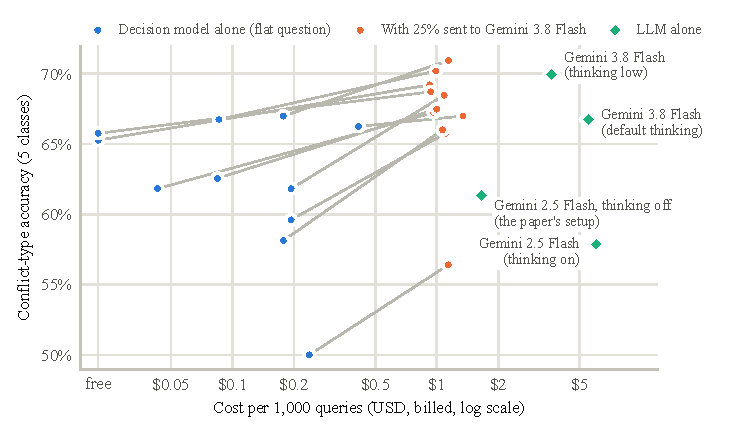
\includegraphics[width=0.78\textwidth]{figures/cascade_cost_accuracy.pdf}
\caption{Accuracy against cost (log scale) on the test split. Curves: \jev answers first and the least confident
fraction of queries goes to Gemini~3.8 Flash; dots mark 25\% and 50\% escalated (at 25\% the two curves nearly
coincide). Diamonds: LLMs alone with the paper's prompt.}
\label{fig:cascade}
\end{figure*}

\subsection{Diagnostics}
\label{sec:diagnostics}

We specified three hypotheses and their tests before running them; Tables~\ref{tab:diagnostics}
and~\ref{tab:plant} give the results. An identical rerun sets the noise floor: no system is deterministic, and
\jev changes its predicted type on \diagjfrerunflip\% of queries with nothing changed (Gemini~3.8 Flash:
\diaggmrerunflip\%).

\begin{table*}[t]
\centering\footnotesize\setlength{\tabcolsep}{4pt}
\fitwidth{\begin{tabular}{lccccccccc}
\toprule
 & \multicolumn{3}{c}{Jev flat} & \multicolumn{3}{c}{Jev tree v2$^\dagger$} & \multicolumn{3}{c}{Gemini 3.8} \\
\cmidrule(lr){2-4}\cmidrule(lr){5-7}\cmidrule(lr){8-10}
Perturbation & $\Delta$Acc ($p$) & Flip & Outd. & $\Delta$Acc ($p$) & Flip & Outd. & $\Delta$Acc ($p$) & Flip & Outd. \\
\midrule
Rerun & $-$0.5 (0.69) & 2.0 & 74.5 & $-$0.2 (1.00) & 2.5 & 20.0 & +1.2 (0.27) & 3.4 & 72.7 \\
No dates & $-$1.0 (0.34) & 3.0 & 74.5 & +0.0 (1.00) & 3.4 & 20.0 & $-$0.7 (0.51) & 2.7 & 67.3 \\
Recency in code & +0.2 (1.00) & 3.4 & 76.4 & +0.2 (1.00) & 3.7 & 21.8 & $-$0.7 (0.65) & 5.7 & 72.7 \\
Shuffle, seed 1 & +1.5 (0.38) & 11.1 & 72.7 & $-$1.5 (0.33) & 9.9 & 18.2 & $-$0.5 (0.85) & 8.4 & 74.5 \\
Shuffle, seed 2 & +0.2 (1.00) & 12.1 & 67.3 & $-$2.2 (0.11) & 8.4 & 18.2 & $-$2.7 (0.09) & 10.3 & 70.9 \\
\midrule
Original Outd.\ recall & \multicolumn{3}{c}{72.7} & \multicolumn{3}{c}{20.0} & \multicolumn{3}{c}{69.1} \\
\bottomrule
\end{tabular}}
\caption{Diagnostics on the test split. Each perturbed run is compared with the same system's original run. $\Delta$Acc: accuracy change in points (exact McNemar $p$). Flip: share of queries whose predicted type changed (\%). Outd.: recall (\%) on the 55 \emph{Outdated} queries after the perturbation. The identical rerun is the noise floor. $^\dagger$Revised on development data.}
\label{tab:diagnostics}
\end{table*}


\paragraph{Dates do not matter.} \jev's documentation lists ordering dates as a known weakness
\citep{typesafe2026jagged}, and we expected it to explain errors on \emph{Outdated}. It does not. Removing every
date changes no system's accuracy beyond the noise floor (\jev: \diagjfnodatesdiff points, $p\diagjfnodatesp$;
Gemini: \diaggmnodatesdiff, $p\diaggmnodatesp$), and neither does adding each result's recency rank computed in
code. \jev's recall on \emph{Outdated} is \diagjforigrec\% originally, \diagjfnodatesrec\% without dates and
\diagjfdatesincoderec\% with code-computed recency, at or above Gemini's in every condition. The systems recognise
outdated sources from their content (phrases such as ``former'' or ``as of'', and conflicting values), not from
publication dates. The weak \emph{Outdated} score of tree v2 comes from its question design, not from dates.

\paragraph{Order sensitivity is real but not specific to \jev.} Shuffling the results changes \jev's predicted type
on \diagjfshuffleflip\% of queries [\diagjfshufflelo, \diagjfshufflehi] over both seeds, well above its
\diagjfrerunflip\% noise floor; Gemini~3.8 Flash flips on \diaggmshuffleflip\%
[\diaggmshufflelo, \diaggmshufflehi]. On the same shuffles the two do not differ ($p\diagflipjevvsgonep$ and $p\diagflipjevvsgtwop$). Accuracy moves by at most a few points in either direction.

\begin{table*}[t]
\centering\small
\fitwidth{\begin{tabular}{lccccc}
\toprule
System & Hit & False al. & Youden & Any conflict & AUROC \\
\midrule
Jev 1.13, flat & 66.7 & 17.7 & +0.490 & 85.4 / 41.7 & 0.81 \\
Jev 1.13, tree v2$^\dagger$ & 19.8 & 2.1 & +0.177 & 67.7 / 25.0 & 0.70 \\
Gemini 3.8 Flash (low) & 52.1 & 3.1 & +0.490 & 71.9 / 25.0 & -- \\
\bottomrule
\end{tabular}}
\caption{One planted false source in 96 \emph{No conflict} test queries (expected label: \emph{Misinformation}). Hit: planted copy labelled Misinformation. False al.: clean copy of the same query labelled Misinformation. Youden = hit $-$ false alarm. Any conflict: planted / clean copy not labelled No conflict. AUROC: P(Misinformation) separating planted from clean copies. $^\dagger$Revised on development data.}
\label{tab:plant}
\end{table*}


\paragraph{A planted false source is noticed as well as by the LLM.} \conflicts has too few \emph{Misinformation}
queries to evaluate. We construct them: in \nplant \emph{No conflict} test queries whose gold answer appears in some
result, we rewrite one such result so that it states a plausible wrong answer, produced by a third model
(GPT-4.1-mini) so that neither classifier judges its own text. The expected label becomes \emph{Misinformation}.
Flat \jev labels \plantjfhit\% of planted queries as misinformation against \plantgmhit\% for Gemini~3.8 Flash
($p\planthitp$), but it also does so for \plantjffa\% of the clean versions of the same queries against
\plantgmfa\% ($p\plantfap$). Net of false alarms the two are identical (Youden \plantjfyouden each; difference
\plantyoudendiff [\plantyoudenlo, \plantyoudenhi]). \jev's misinformation probability separates planted from clean
versions with AUROC \plantjfauroc, so a threshold can trade detections for fewer false alarms. Tree v2, whose
misinformation rule was chosen on a development split with a single misinformation query, detects only
\plantjthit\%.

\subsection{Robustness across versions and decision models}
\label{sec:robustness}

\paragraph{\jev 1.14.} The newer version behaves like 1.13 (Table~\ref{tab:main}): \onefouracc\% with the flat
question (\onefourvsonethreediff points, $p\onefourvsonethreep$) and \onefourtreeacc\% with tree v2
($p\onefourtreevsonethreep$), still tied with Gemini~2.5 Flash ($p\onefourvstwofivep$), with the same failure
of tree v1 and the same cascade behaviour (tree v2 at 50\%: \onefourcascfiftyacc\%, $p\onefourcascfiftyp$ against
the LLM alone).

\begin{table*}[t]
\centering\small\setlength{\tabcolsep}{5pt}
\fitwidth{\begin{tabular}{lccccccc}
\toprule
Decision model & Flat & Tree v2 & ECE & \$ / 1k & Lat.\ (s) & $\Delta$ Jev ($p$) & $\Delta$ Gemini 3.8 ($p$) \\
\midrule
Jev 1.13 & 61.8 & 63.5 & 0.103 & 0.19 & 0.26 & -- & $-$8.1 ({<}0.001) \\
Perplexity v1.2 & 66.7 & 69.0 & 0.061 & 0.09 & 0.42 & +4.9 (0.03) & $-$3.2 (0.14) \\
GPT-6-luna & 66.3 & 50.0 & 0.059 & 0.41 & 0.35 & +4.4 (0.11) & $-$3.7 (0.13) \\
Liquid d1 & 62.6 & 58.4 & 0.075 & 0.08 & 0.41 & +0.7 (0.83) & $-$7.4 (0.002) \\
Microsoft d-1 & 58.1 & 57.4 & 0.188 & 0.18 & 0.45 & $-$3.7 (0.13) & $-$11.8 ({<}0.001) \\
\bottomrule
\end{tabular}}
\caption{Jev against the other decision models available through the same gateway, with Jev's frozen questions and inputs, nothing tuned per model (test split). Flat, Tree v2: accuracy (\%). ECE and latency for the flat question. $\Delta$: accuracy difference of the flat question from Jev and from Gemini~3.8 Flash in points, with exact McNemar $p$. Models: Perplexity decider v1.2, OpenAI GPT-6-luna decisions, Liquid d1, Microsoft decision-1. Gemini 3.8 Flash (thinking low) scores 70.0\% at \$3.65 per 1k queries.}
\label{tab:decision_models}
\end{table*}


\paragraph{Other decision models.} Table~\ref{tab:decision_models} places \jev among the decision models
available through the same gateway. \jev is mid-pack in accuracy and the fastest. Perplexity's decider is the most
accurate: \pplxflatacc\% with the flat question, \pplxvsjevdiffabs points above \jev ($p\pplxvsjevp$), and
\pplxtreeacc\% with tree v2, statistically tied with Gemini~3.8 Flash ($p\pplxtreevsgp$). As a cascade first
stage it reaches \cascpplxtfacc\% at \cascpplxtfcost\% of the LLM's cost at $f=25\%$. Not every decision model's
confidence is useful for escalation: GPT-6-luna's confidence barely ranks its errors (AUROC \lunaauroc), and its
25\% cascade is no better than random escalation (\lunacasctf\% vs.\ \lunacasctfrand\%).

\section{Discussion}
\label{sec:discussion}

\paragraph{What decision models offer as conflict classifiers.} Conflict typing sits on the critical path of every
search-augmented answer, so its latency and cost add to every request. Most hosted decision models classify a query
with about ten retrieved pages in under half a second, for at most \$\dmcostmax per thousand queries, with the accuracy of the LLM used in the original study. When the accuracy of a
current LLM is required, a decision model's confidence is usually good enough to route only its uncertain queries to
the LLM, which recovers most of the gap at a quarter to a third of the LLM's cost. End to end, the cheaper types cost
no measurable answer quality (\S\ref{sec:endtoend}). 

\paragraph{Choosing among decision models.} The class is not uniform. Accuracy spans \dmaccmin--\dmaccmax\%, and the
model at the bottom is significantly worse than the paper's LLM. Two properties that matter in deployment vary
independently of accuracy: calibration (ECE \eceminimum--\ecemaximum) and how well confidence ranks errors, which
decides whether a cascade helps at all. One of the most accurate models has confidence that is no better than random for
escalation. A model for this task should therefore be chosen on all three, measured on the deployment's own data,
not on accuracy alone.

\paragraph{How to ask.} The direct choice question was the reliable format for every model. The yes/no
decomposition looked natural but failed for all of them; the repaired tree encodes choices fitted to one model on a
small development split and did not help any other. For a new decision model we would start from the flat
question.

\paragraph{What the diagnostics change.} Dates turned out not to matter: outdated sources are recognised
from their content. Sensitivity to source order is real but differs so much between models that it has to be
measured for each one. A single false source is the subtle case, visible in the probabilities but rarely in the
top label. With
\nmisitest natural \emph{Misinformation} test queries, that type is the one a deployment would most need to
calibrate on its own data.

\paragraph{Limitations.}
(i) \conflicts is small: with \ntest test queries, differences under about five points are not significant, and the
cascades can be shown close to, but not formally equivalent to, the LLM. (ii) The label distribution reflects how the
queries were selected, not real search traffic, and the dataset has only five natural \emph{Misinformation}
queries; our planted variant tests one kind of misinformation (an entity or value substituted in a single source).
(iii) The census covers the decision models one gateway served on one day. Hosted models change without notice:
several identifiers are unversioned, two models were free during our runs, and our rerun of Gemini~2.5 Flash scores
below the published figure. Providers
do not disclose model sizes or training data, so we cannot explain the differences between models. (iv) The end-to-end test uses one generator and LLM judges, validated on \nvalid answers, that do not see the
search results; as in the original study, the primary judge is the generator's own model, which may favour its
answers \citep{panickssery2024llm}. The size of the gain from predicted types depends on the judge, and we do not
measure factual grounding, the third metric of \citet{cattan2025dragged}. (v) Not every system is deterministic: identical requests changed
up to \rerunflipmax\% of a decision model's predictions, and \diaggmrerunflip\% of Gemini~3.8 Flash's.

\section{Conclusion}
\label{sec:conclusion}

We tested every typed decision model hosted on one gateway as a classifier of knowledge-conflict types, using
the benchmark authors' protocol and the same inputs as the LLMs. Most match the LLM of the original study. They do
so at a small fraction of its cost and latency. They trail the
current LLM, but for most of them a confidence-gated cascade recovers that gap at a quarter to a third of the LLM's
cost, and given to a generator, their types yield answers that follow the expected behaviour as often as the LLM's.
 Future work should measure the gain from predicted types with judges that see the
sources, and test whether a decision model's probabilities can steer a generator between expected behaviours when
the type is uncertain.

\section*{Ethics and Broader Impact}

The planted-misinformation variant rewrites one retrieved page per query to state a wrong answer. It uses public data and factual substitutions on
non-sensitive questions, and is released with clear labels. All queries in \conflicts are safe by construction \citep{cattan2025dragged}. Cheap conflict
classification could be misused to suppress minority viewpoints; the expected behaviour for \emph{Conflicting
opinions} is to present all of them.


\bibliography{refs}
\bibliographystyle{acl_natbib}

\appendix
\section{Prompts and Questions}
\label{app:prompts}

\paragraph{LLM prompt.} The conflict-type prompt of \citet{cattan2025dragged}, copied from the paper's source with
only the \LaTeX{} bold markers removed. \texttt{\{search\_results\}} is filled with the numbered results.

\lstinputlisting{generated/paper_prompt.txt}

\paragraph{\jev, flat.} One choice question. Its instruction is the first paragraph of the prompt above; its options
are the five category definitions with their examples, word for word.

\lstinputlisting{generated/flat_question.txt}

\paragraph{\jev, tree.} Five yes/no questions asked in one request over the same state.

\lstinputlisting{generated/tree_questions.txt}

\paragraph{Planted wrong answers.} Prompt sent to GPT-4.1-mini (temperature 0) to obtain a plausible wrong answer
for each \emph{No conflict} query whose gold answer appears in a result. The answer is then replaced, as whole words
and case-insensitively, in the title, snippet and text of one such result chosen with a fixed seed. Queries whose
gold answer is \emph{yes} or \emph{no} are excluded.

\lstinputlisting{generated/wrong_answer_prompt.txt}

\section{Protocol Record}
\label{app:protocol}

The development/test split, the prompt and question texts and the combination rules were frozen with recorded file
hashes before any test-set call. Changes after that point were limited to the following, each logged with its reason
before results were computed: (1) Gemini~2.5 Flash with thinking added as a sensitivity check; (2) the answer parser
made lenient for category statements outside the requested JSON, applied to stored answers without new calls (no
strictly formatted answer changed); (3) Gemini~3.8 Flash added at two thinking levels; (4) the cascade, its
operating points and its controls; (5) the diagnostics, with one amendment before any planted run: whole-word
matching and the exclusion of yes/no answers, after substring matching was found to alter unrelated numbers;
(6) \jev 1.14 and the four other decision models, run with \jev's frozen questions. All runs were reported. Code,
splits, prompts, cached responses and per-query outputs are released.


\end{document}
"
%   arXiv preprint:        scripts/make_arxiv.sh  (authors shown, no line numbers or header)
\ifdefined\taclfinal\def\taclauthors{}\fi
\ifdefined\arxivversion\def\taclauthors{}\fi
\ifdefined\taclauthors\usepackage[acceptedWithA]{tacl2021v1}\else\usepackage{tacl2021v1}\fi
% The author block needs more than the style's default 5 cm title box (its own advice: set \titlebox right
% after loading the style). Not needed for the anonymous submission.
\ifdefined\taclauthors\setlength\titlebox{6.5cm}\fi
% PDF metadata: title always; authors only in the builds that show them.
\hypersetup{pdftitle={Do We Need an LLM to Know Why Sources Conflict? Decision Models for Knowledge-Conflict Typing in RAG}}
\ifdefined\taclauthors\hypersetup{pdfauthor={Parv Khatri, Harshul Jain, Mehak Kapoor, Tanya Sah}}\fi
% Code release: linked only in the versions that show authors (arXiv, camera-ready). The anonymous
% TACL submission may not link to code, so it only says that everything is released.
\newcommand{\repourl}{https://github.com/Parv17k/decision-models-conflict-typing}
\ifdefined\taclauthors\newcommand{\releasenote}{ at \url{\repourl}}\else\newcommand{\releasenote}{}\fi
\usepackage{xspace}
\xspaceaddexceptions{\% $ ] ) / , ;}   % no space between a generated number and %, $, brackets or punctuation
\usepackage{booktabs}
\usepackage{graphicx}
\usepackage{amsmath}
\usepackage{xcolor}
\usepackage{tikz}
\usepackage{listings}

\lstset{basicstyle=\scriptsize\ttfamily,breaklines=true,breakatwhitespace=true,columns=fullflexible,
        frame=single,framerule=0.4pt,rulecolor=\color{gray},xleftmargin=2pt,xrightmargin=2pt}
% Shrink a table to the line width only if it is wider (graphicx only; no adjustbox in BasicTeX).
\newsavebox{\fitbox}
\newcommand{\fitwidth}[1]{\sbox{\fitbox}{#1}\ifdim\wd\fitbox>\linewidth\typeout{FITWIDTH scaled \the\wd\fitbox\space to \the\linewidth}\resizebox{\linewidth}{!}{\usebox{\fitbox}}\else\usebox{\fitbox}\fi}
% References ragged-right: in a justified narrow column, long URLs otherwise stretch with visible gaps.
\makeatletter\let\dm@thebibliography\thebibliography
\renewcommand{\thebibliography}[1]{\dm@thebibliography{#1}\raggedright}\makeatother
\newcommand{\todo}[1]{\textcolor{orange!80!black}{[TODO: #1]}}
\newcommand{\jev}{Jev\xspace}
\newcommand{\conflicts}{\textsc{Conflicts}\xspace}

% Generated by scripts/make_tables.py from the stored runs. Do not edit.
\newcommand{\allgtwofive}{60.7\xspace}
\newcommand{\aurocmax}{0.76\xspace}
\newcommand{\aurocmin}{0.64\xspace}
\newcommand{\avgresults}{9.2\xspace}
\newcommand{\cascelephantfiftyacc}{70.0\xspace}
\newcommand{\cascelephantfiftycost}{50\xspace}
\newcommand{\cascelephantfiftydiff}{+0.0\xspace}
\newcommand{\cascelephantfiftydiffabs}{0.0\xspace}
\newcommand{\cascelephantfiftyhi}{+2.0\xspace}
\newcommand{\cascelephantfiftyhiabs}{2.0\xspace}
\newcommand{\cascelephantfiftylat}{1.59\xspace}
\newcommand{\cascelephantfiftylo}{$-$2.0\xspace}
\newcommand{\cascelephantfiftyloabs}{2.0\xspace}
\newcommand{\cascelephantfiftyp}{=1.00\xspace}
\newcommand{\cascelephantfiftyrand}{67.6\xspace}
\newcommand{\cascelephanttfacc}{69.2\xspace}
\newcommand{\cascelephanttfcost}{25\xspace}
\newcommand{\cascelephanttfdiff}{$-$0.7\xspace}
\newcommand{\cascelephanttfdiffabs}{0.7\xspace}
\newcommand{\cascelephanttfhi}{+2.5\xspace}
\newcommand{\cascelephanttfhiabs}{2.5\xspace}
\newcommand{\cascelephanttflat}{1.02\xspace}
\newcommand{\cascelephanttflo}{$-$3.9\xspace}
\newcommand{\cascelephanttfloabs}{3.9\xspace}
\newcommand{\cascelephanttfp}{=0.77\xspace}
\newcommand{\cascelephanttfrand}{66.4\xspace}
\newcommand{\cascgainmax}{4.9\xspace}
\newcommand{\cascgainmin}{-0.2\xspace}
\newcommand{\cascjevfiftyacc}{69.2\xspace}
\newcommand{\cascjevfiftycost}{54\xspace}
\newcommand{\cascjevfiftydiff}{$-$0.7\xspace}
\newcommand{\cascjevfiftydiffabs}{0.7\xspace}
\newcommand{\cascjevfiftyhi}{+1.0\xspace}
\newcommand{\cascjevfiftyhiabs}{1.0\xspace}
\newcommand{\cascjevfiftylat}{1.34\xspace}
\newcommand{\cascjevfiftylo}{$-$2.7\xspace}
\newcommand{\cascjevfiftyloabs}{2.7\xspace}
\newcommand{\cascjevfiftyp}{=0.61\xspace}
\newcommand{\cascjevfiftyrand}{65.9\xspace}
\newcommand{\cascjevnewfiftyacc}{68.7\xspace}
\newcommand{\cascjevnewfiftycost}{54\xspace}
\newcommand{\cascjevnewfiftydiff}{$-$1.2\xspace}
\newcommand{\cascjevnewfiftydiffabs}{1.2\xspace}
\newcommand{\cascjevnewfiftyhi}{+1.0\xspace}
\newcommand{\cascjevnewfiftyhiabs}{1.0\xspace}
\newcommand{\cascjevnewfiftylat}{1.36\xspace}
\newcommand{\cascjevnewfiftylo}{$-$3.4\xspace}
\newcommand{\cascjevnewfiftyloabs}{3.4\xspace}
\newcommand{\cascjevnewfiftyp}{=0.36\xspace}
\newcommand{\cascjevnewfiftyrand}{64.8\xspace}
\newcommand{\cascjevnewtfacc}{65.8\xspace}
\newcommand{\cascjevnewtfcost}{30\xspace}
\newcommand{\cascjevnewtfdiff}{$-$4.2\xspace}
\newcommand{\cascjevnewtfdiffabs}{4.2\xspace}
\newcommand{\cascjevnewtfhi}{$-$1.0\xspace}
\newcommand{\cascjevnewtfhiabs}{1.0\xspace}
\newcommand{\cascjevnewtflat}{0.82\xspace}
\newcommand{\cascjevnewtflo}{$-$7.4\xspace}
\newcommand{\cascjevnewtfloabs}{7.4\xspace}
\newcommand{\cascjevnewtfp}{=0.016\xspace}
\newcommand{\cascjevnewtfrand}{62.2\xspace}
\newcommand{\cascjevtfacc}{68.5\xspace}
\newcommand{\cascjevtfcost}{30\xspace}
\newcommand{\cascjevtfdiff}{$-$1.5\xspace}
\newcommand{\cascjevtfdiffabs}{1.5\xspace}
\newcommand{\cascjevtfhi}{+1.5\xspace}
\newcommand{\cascjevtfhiabs}{1.5\xspace}
\newcommand{\cascjevtflat}{0.81\xspace}
\newcommand{\cascjevtflo}{$-$4.4\xspace}
\newcommand{\cascjevtfloabs}{4.4\xspace}
\newcommand{\cascjevtfp}{=0.41\xspace}
\newcommand{\cascjevtfrand}{63.9\xspace}
\newcommand{\cascliquidfiftyacc}{69.2\xspace}
\newcommand{\cascliquidfiftycost}{52\xspace}
\newcommand{\cascliquidfiftydiff}{$-$0.7\xspace}
\newcommand{\cascliquidfiftydiffabs}{0.7\xspace}
\newcommand{\cascliquidfiftyhi}{+0.7\xspace}
\newcommand{\cascliquidfiftyhiabs}{0.7\xspace}
\newcommand{\cascliquidfiftylat}{1.51\xspace}
\newcommand{\cascliquidfiftylo}{$-$2.5\xspace}
\newcommand{\cascliquidfiftyloabs}{2.5\xspace}
\newcommand{\cascliquidfiftyp}{=0.55\xspace}
\newcommand{\cascliquidfiftyrand}{66.3\xspace}
\newcommand{\cascliquidtfacc}{67.5\xspace}
\newcommand{\cascliquidtfcost}{27\xspace}
\newcommand{\cascliquidtfdiff}{$-$2.5\xspace}
\newcommand{\cascliquidtfdiffabs}{2.5\xspace}
\newcommand{\cascliquidtfhi}{+0.5\xspace}
\newcommand{\cascliquidtfhiabs}{0.5\xspace}
\newcommand{\cascliquidtflat}{0.97\xspace}
\newcommand{\cascliquidtflo}{$-$5.4\xspace}
\newcommand{\cascliquidtfloabs}{5.4\xspace}
\newcommand{\cascliquidtfp}{=0.14\xspace}
\newcommand{\cascliquidtfrand}{64.4\xspace}
\newcommand{\cascliquidultrafiftyacc}{70.4\xspace}
\newcommand{\cascliquidultrafiftycost}{55\xspace}
\newcommand{\cascliquidultrafiftydiff}{+0.5\xspace}
\newcommand{\cascliquidultrafiftydiffabs}{0.5\xspace}
\newcommand{\cascliquidultrafiftyhi}{+2.2\xspace}
\newcommand{\cascliquidultrafiftyhiabs}{2.2\xspace}
\newcommand{\cascliquidultrafiftylat}{1.59\xspace}
\newcommand{\cascliquidultrafiftylo}{$-$1.2\xspace}
\newcommand{\cascliquidultrafiftyloabs}{1.2\xspace}
\newcommand{\cascliquidultrafiftyp}{=0.77\xspace}
\newcommand{\cascliquidultrafiftyrand}{68.5\xspace}
\newcommand{\cascliquidultratfacc}{70.9\xspace}
\newcommand{\cascliquidultratfcost}{31\xspace}
\newcommand{\cascliquidultratfdiff}{+1.0\xspace}
\newcommand{\cascliquidultratfdiffabs}{1.0\xspace}
\newcommand{\cascliquidultratfhi}{+3.9\xspace}
\newcommand{\cascliquidultratfhiabs}{3.9\xspace}
\newcommand{\cascliquidultratflat}{1.05\xspace}
\newcommand{\cascliquidultratflo}{$-$2.0\xspace}
\newcommand{\cascliquidultratfloabs}{2.0\xspace}
\newcommand{\cascliquidultratfp}{=0.63\xspace}
\newcommand{\cascliquidultratfrand}{67.7\xspace}
\newcommand{\casclunafiftyacc}{69.0\xspace}
\newcommand{\casclunafiftycost}{61\xspace}
\newcommand{\casclunafiftydiff}{$-$1.0\xspace}
\newcommand{\casclunafiftydiffabs}{1.0\xspace}
\newcommand{\casclunafiftyhi}{+1.0\xspace}
\newcommand{\casclunafiftyhiabs}{1.0\xspace}
\newcommand{\casclunafiftylat}{1.42\xspace}
\newcommand{\casclunafiftylo}{$-$3.0\xspace}
\newcommand{\casclunafiftyloabs}{3.0\xspace}
\newcommand{\casclunafiftyp}{=0.48\xspace}
\newcommand{\casclunafiftyrand}{68.1\xspace}
\newcommand{\casclunatfacc}{67.0\xspace}
\newcommand{\casclunatfcost}{37\xspace}
\newcommand{\casclunatfdiff}{$-$3.0\xspace}
\newcommand{\casclunatfdiffabs}{3.0\xspace}
\newcommand{\casclunatfhi}{+0.2\xspace}
\newcommand{\casclunatfhiabs}{0.2\xspace}
\newcommand{\casclunatflat}{0.89\xspace}
\newcommand{\casclunatflo}{$-$6.2\xspace}
\newcommand{\casclunatfloabs}{6.2\xspace}
\newcommand{\casclunatfp}{=0.10\xspace}
\newcommand{\casclunatfrand}{67.2\xspace}
\newcommand{\cascmammothfiftyacc}{70.2\xspace}
\newcommand{\cascmammothfiftycost}{50\xspace}
\newcommand{\cascmammothfiftydiff}{+0.2\xspace}
\newcommand{\cascmammothfiftydiffabs}{0.2\xspace}
\newcommand{\cascmammothfiftyhi}{+1.7\xspace}
\newcommand{\cascmammothfiftyhiabs}{1.7\xspace}
\newcommand{\cascmammothfiftylat}{1.71\xspace}
\newcommand{\cascmammothfiftylo}{$-$1.2\xspace}
\newcommand{\cascmammothfiftyloabs}{1.2\xspace}
\newcommand{\cascmammothfiftyp}{=1.00\xspace}
\newcommand{\cascmammothfiftyrand}{67.9\xspace}
\newcommand{\cascmammothtfacc}{68.7\xspace}
\newcommand{\cascmammothtfcost}{26\xspace}
\newcommand{\cascmammothtfdiff}{$-$1.2\xspace}
\newcommand{\cascmammothtfdiffabs}{1.2\xspace}
\newcommand{\cascmammothtfhi}{+1.5\xspace}
\newcommand{\cascmammothtfhiabs}{1.5\xspace}
\newcommand{\cascmammothtflat}{1.18\xspace}
\newcommand{\cascmammothtflo}{$-$3.9\xspace}
\newcommand{\cascmammothtfloabs}{3.9\xspace}
\newcommand{\cascmammothtfp}{=0.49\xspace}
\newcommand{\cascmammothtfrand}{66.8\xspace}
\newcommand{\cascmsftfiftyacc}{69.2\xspace}
\newcommand{\cascmsftfiftycost}{54\xspace}
\newcommand{\cascmsftfiftydiff}{$-$0.7\xspace}
\newcommand{\cascmsftfiftydiffabs}{0.7\xspace}
\newcommand{\cascmsftfiftyhi}{+1.2\xspace}
\newcommand{\cascmsftfiftyhiabs}{1.2\xspace}
\newcommand{\cascmsftfiftylat}{1.54\xspace}
\newcommand{\cascmsftfiftylo}{$-$3.0\xspace}
\newcommand{\cascmsftfiftyloabs}{3.0\xspace}
\newcommand{\cascmsftfiftyp}{=0.65\xspace}
\newcommand{\cascmsftfiftyrand}{64.0\xspace}
\newcommand{\cascmsfttfacc}{66.0\xspace}
\newcommand{\cascmsfttfcost}{29\xspace}
\newcommand{\cascmsfttfdiff}{$-$3.9\xspace}
\newcommand{\cascmsfttfdiffabs}{3.9\xspace}
\newcommand{\cascmsfttfhi}{$-$0.5\xspace}
\newcommand{\cascmsfttfhiabs}{0.5\xspace}
\newcommand{\cascmsfttflat}{0.97\xspace}
\newcommand{\cascmsfttflo}{$-$7.6\xspace}
\newcommand{\cascmsfttfloabs}{7.6\xspace}
\newcommand{\cascmsfttfp}{=0.048\xspace}
\newcommand{\cascmsfttfrand}{61.1\xspace}
\newcommand{\cascpplxfiftyacc}{70.0\xspace}
\newcommand{\cascpplxfiftycost}{52\xspace}
\newcommand{\cascpplxfiftydiff}{+0.0\xspace}
\newcommand{\cascpplxfiftydiffabs}{0.0\xspace}
\newcommand{\cascpplxfiftyhi}{+1.5\xspace}
\newcommand{\cascpplxfiftyhiabs}{1.5\xspace}
\newcommand{\cascpplxfiftylat}{1.54\xspace}
\newcommand{\cascpplxfiftylo}{$-$1.5\xspace}
\newcommand{\cascpplxfiftyloabs}{1.5\xspace}
\newcommand{\cascpplxfiftyp}{=1.00\xspace}
\newcommand{\cascpplxfiftyrand}{68.3\xspace}
\newcommand{\cascpplxflashfiftyacc}{68.5\xspace}
\newcommand{\cascpplxflashfiftycost}{51\xspace}
\newcommand{\cascpplxflashfiftydiff}{$-$1.5\xspace}
\newcommand{\cascpplxflashfiftydiffabs}{1.5\xspace}
\newcommand{\cascpplxflashfiftyhi}{+0.7\xspace}
\newcommand{\cascpplxflashfiftyhiabs}{0.7\xspace}
\newcommand{\cascpplxflashfiftylat}{1.43\xspace}
\newcommand{\cascpplxflashfiftylo}{$-$3.7\xspace}
\newcommand{\cascpplxflashfiftyloabs}{3.7\xspace}
\newcommand{\cascpplxflashfiftyp}{=0.26\xspace}
\newcommand{\cascpplxflashfiftyrand}{65.9\xspace}
\newcommand{\cascpplxflashtfacc}{67.2\xspace}
\newcommand{\cascpplxflashtfcost}{26\xspace}
\newcommand{\cascpplxflashtfdiff}{$-$2.7\xspace}
\newcommand{\cascpplxflashtfdiffabs}{2.7\xspace}
\newcommand{\cascpplxflashtfhi}{+0.2\xspace}
\newcommand{\cascpplxflashtfhiabs}{0.2\xspace}
\newcommand{\cascpplxflashtflat}{0.87\xspace}
\newcommand{\cascpplxflashtflo}{$-$5.9\xspace}
\newcommand{\cascpplxflashtfloabs}{5.9\xspace}
\newcommand{\cascpplxflashtfp}{=0.13\xspace}
\newcommand{\cascpplxflashtfrand}{63.9\xspace}
\newcommand{\cascpplxtfacc}{70.2\xspace}
\newcommand{\cascpplxtfcost}{27\xspace}
\newcommand{\cascpplxtfdiff}{+0.2\xspace}
\newcommand{\cascpplxtfdiffabs}{0.2\xspace}
\newcommand{\cascpplxtfhi}{+2.7\xspace}
\newcommand{\cascpplxtfhiabs}{2.7\xspace}
\newcommand{\cascpplxtflat}{0.97\xspace}
\newcommand{\cascpplxtflo}{$-$2.2\xspace}
\newcommand{\cascpplxtfloabs}{2.2\xspace}
\newcommand{\cascpplxtfp}{=1.00\xspace}
\newcommand{\cascpplxtfrand}{67.6\xspace}
\newcommand{\cascscaledownfiftyacc}{62.8\xspace}
\newcommand{\cascscaledownfiftycost}{57\xspace}
\newcommand{\cascscaledownfiftydiff}{$-$7.1\xspace}
\newcommand{\cascscaledownfiftydiffabs}{7.1\xspace}
\newcommand{\cascscaledownfiftyhi}{$-$3.7\xspace}
\newcommand{\cascscaledownfiftyhiabs}{3.7\xspace}
\newcommand{\cascscaledownfiftylat}{1.83\xspace}
\newcommand{\cascscaledownfiftylo}{$-$10.8\xspace}
\newcommand{\cascscaledownfiftyloabs}{10.8\xspace}
\newcommand{\cascscaledownfiftyp}{<0.001\xspace}
\newcommand{\cascscaledownfiftyrand}{60.0\xspace}
\newcommand{\cascscaledowntfacc}{56.4\xspace}
\newcommand{\cascscaledowntfcost}{31\xspace}
\newcommand{\cascscaledowntfdiff}{$-$13.5\xspace}
\newcommand{\cascscaledowntfdiffabs}{13.5\xspace}
\newcommand{\cascscaledowntfhi}{$-$8.9\xspace}
\newcommand{\cascscaledowntfhiabs}{8.9\xspace}
\newcommand{\cascscaledowntflat}{1.29\xspace}
\newcommand{\cascscaledowntflo}{$-$18.0\xspace}
\newcommand{\cascscaledowntfloabs}{18.0\xspace}
\newcommand{\cascscaledowntfp}{<0.001\xspace}
\newcommand{\cascscaledowntfrand}{55.0\xspace}
\newcommand{\casctiedcostmax}{37\xspace}
\newcommand{\casctiedcostmin}{25\xspace}
\newcommand{\cihalf}{4.8\xspace}
\newcommand{\costratiorefmax}{39\xspace}
\newcommand{\costratiorefmin}{4\xspace}
\newcommand{\costratiorefnow}{2.2\xspace}
\newcommand{\devcompatcomp}{0.81\xspace}
\newcommand{\devcompatopin}{0.69\xspace}
\newcommand{\devmisinfohi}{0.79\xspace}
\newcommand{\devmisinfolo}{0.53\xspace}
\newcommand{\devnopin}{13\xspace}
\newcommand{\devopinionauroc}{0.83\xspace}
\newcommand{\devopintocomp}{12\xspace}
\newcommand{\diagelephantdatesincodediff}{+0.7\xspace}
\newcommand{\diagelephantdatesincodediffabs}{0.7\xspace}
\newcommand{\diagelephantdatesincodehi}{+2.5\xspace}
\newcommand{\diagelephantdatesincodehiabs}{2.5\xspace}
\newcommand{\diagelephantdatesincodelo}{$-$0.7\xspace}
\newcommand{\diagelephantdatesincodeloabs}{0.7\xspace}
\newcommand{\diagelephantdatesincodep}{=0.55\xspace}
\newcommand{\diagelephantdatesincoderec}{58.2\xspace}
\newcommand{\diagelephantnodatesdiff}{+0.5\xspace}
\newcommand{\diagelephantnodatesdiffabs}{0.5\xspace}
\newcommand{\diagelephantnodateshi}{+2.5\xspace}
\newcommand{\diagelephantnodateshiabs}{2.5\xspace}
\newcommand{\diagelephantnodateslo}{$-$1.5\xspace}
\newcommand{\diagelephantnodatesloabs}{1.5\xspace}
\newcommand{\diagelephantnodatesp}{=0.80\xspace}
\newcommand{\diagelephantnodatesrec}{65.5\xspace}
\newcommand{\diagelephantorigrec}{56.4\xspace}
\newcommand{\diagelephantrerunflip}{0.0\xspace}
\newcommand{\diagelephantshuffleflip}{7.3\xspace}
\newcommand{\diagelephantshufflehi}{9.1\xspace}
\newcommand{\diagelephantshufflelo}{5.5\xspace}
\newcommand{\diagelephantshuffleonediff}{$-$0.7\xspace}
\newcommand{\diagelephantshuffleonediffabs}{0.7\xspace}
\newcommand{\diagelephantshuffleonehi}{+1.5\xspace}
\newcommand{\diagelephantshuffleonehiabs}{1.5\xspace}
\newcommand{\diagelephantshuffleonelo}{$-$3.0\xspace}
\newcommand{\diagelephantshuffleoneloabs}{3.0\xspace}
\newcommand{\diagelephantshuffleonep}{=0.68\xspace}
\newcommand{\diagelephantshuffletwodiff}{$-$1.0\xspace}
\newcommand{\diagelephantshuffletwodiffabs}{1.0\xspace}
\newcommand{\diagelephantshuffletwohi}{+1.0\xspace}
\newcommand{\diagelephantshuffletwohiabs}{1.0\xspace}
\newcommand{\diagelephantshuffletwolo}{$-$3.0\xspace}
\newcommand{\diagelephantshuffletwoloabs}{3.0\xspace}
\newcommand{\diagelephantshuffletwop}{=0.48\xspace}
\newcommand{\diaggmdatesincodediff}{$-$0.7\xspace}
\newcommand{\diaggmdatesincodediffabs}{0.7\xspace}
\newcommand{\diaggmdatesincodehi}{+1.5\xspace}
\newcommand{\diaggmdatesincodehiabs}{1.5\xspace}
\newcommand{\diaggmdatesincodelo}{$-$2.7\xspace}
\newcommand{\diaggmdatesincodeloabs}{2.7\xspace}
\newcommand{\diaggmdatesincodep}{=0.65\xspace}
\newcommand{\diaggmdatesincoderec}{72.7\xspace}
\newcommand{\diaggmnodatesdiff}{$-$0.7\xspace}
\newcommand{\diaggmnodatesdiffabs}{0.7\xspace}
\newcommand{\diaggmnodateshi}{+0.7\xspace}
\newcommand{\diaggmnodateshiabs}{0.7\xspace}
\newcommand{\diaggmnodateslo}{$-$2.2\xspace}
\newcommand{\diaggmnodatesloabs}{2.2\xspace}
\newcommand{\diaggmnodatesp}{=0.51\xspace}
\newcommand{\diaggmnodatesrec}{67.3\xspace}
\newcommand{\diaggmorigrec}{69.1\xspace}
\newcommand{\diaggmrerunflip}{3.4\xspace}
\newcommand{\diaggmshuffleflip}{9.4\xspace}
\newcommand{\diaggmshufflehi}{11.5\xspace}
\newcommand{\diaggmshufflelo}{7.5\xspace}
\newcommand{\diagjevdatesincodediff}{+0.2\xspace}
\newcommand{\diagjevdatesincodediffabs}{0.2\xspace}
\newcommand{\diagjevdatesincodehi}{+1.7\xspace}
\newcommand{\diagjevdatesincodehiabs}{1.7\xspace}
\newcommand{\diagjevdatesincodelo}{$-$1.2\xspace}
\newcommand{\diagjevdatesincodeloabs}{1.2\xspace}
\newcommand{\diagjevdatesincodep}{=1.00\xspace}
\newcommand{\diagjevdatesincoderec}{76.4\xspace}
\newcommand{\diagjevnewdatesincodediff}{+1.0\xspace}
\newcommand{\diagjevnewdatesincodediffabs}{1.0\xspace}
\newcommand{\diagjevnewdatesincodehi}{+2.7\xspace}
\newcommand{\diagjevnewdatesincodehiabs}{2.7\xspace}
\newcommand{\diagjevnewdatesincodelo}{$-$0.7\xspace}
\newcommand{\diagjevnewdatesincodeloabs}{0.7\xspace}
\newcommand{\diagjevnewdatesincodep}{=0.39\xspace}
\newcommand{\diagjevnewdatesincoderec}{80.0\xspace}
\newcommand{\diagjevnewnodatesdiff}{+0.0\xspace}
\newcommand{\diagjevnewnodatesdiffabs}{0.0\xspace}
\newcommand{\diagjevnewnodateshi}{+1.2\xspace}
\newcommand{\diagjevnewnodateshiabs}{1.2\xspace}
\newcommand{\diagjevnewnodateslo}{$-$1.2\xspace}
\newcommand{\diagjevnewnodatesloabs}{1.2\xspace}
\newcommand{\diagjevnewnodatesp}{=1.00\xspace}
\newcommand{\diagjevnewnodatesrec}{76.4\xspace}
\newcommand{\diagjevneworigrec}{76.4\xspace}
\newcommand{\diagjevnewrerunflip}{3.0\xspace}
\newcommand{\diagjevnewshuffleflip}{10.8\xspace}
\newcommand{\diagjevnewshufflehi}{12.9\xspace}
\newcommand{\diagjevnewshufflelo}{8.7\xspace}
\newcommand{\diagjevnewshuffleonediff}{+1.0\xspace}
\newcommand{\diagjevnewshuffleonediffabs}{1.0\xspace}
\newcommand{\diagjevnewshuffleonehi}{+3.7\xspace}
\newcommand{\diagjevnewshuffleonehiabs}{3.7\xspace}
\newcommand{\diagjevnewshuffleonelo}{$-$1.7\xspace}
\newcommand{\diagjevnewshuffleoneloabs}{1.7\xspace}
\newcommand{\diagjevnewshuffleonep}{=0.60\xspace}
\newcommand{\diagjevnewshuffletwodiff}{+0.0\xspace}
\newcommand{\diagjevnewshuffletwodiffabs}{0.0\xspace}
\newcommand{\diagjevnewshuffletwohi}{+2.5\xspace}
\newcommand{\diagjevnewshuffletwohiabs}{2.5\xspace}
\newcommand{\diagjevnewshuffletwolo}{$-$2.5\xspace}
\newcommand{\diagjevnewshuffletwoloabs}{2.5\xspace}
\newcommand{\diagjevnewshuffletwop}{=1.00\xspace}
\newcommand{\diagjevnodatesdiff}{$-$1.0\xspace}
\newcommand{\diagjevnodatesdiffabs}{1.0\xspace}
\newcommand{\diagjevnodateshi}{+0.5\xspace}
\newcommand{\diagjevnodateshiabs}{0.5\xspace}
\newcommand{\diagjevnodateslo}{$-$2.5\xspace}
\newcommand{\diagjevnodatesloabs}{2.5\xspace}
\newcommand{\diagjevnodatesp}{=0.34\xspace}
\newcommand{\diagjevnodatesrec}{74.5\xspace}
\newcommand{\diagjevorigrec}{72.7\xspace}
\newcommand{\diagjevrerunflip}{2.0\xspace}
\newcommand{\diagjevshuffleflip}{11.6\xspace}
\newcommand{\diagjevshufflehi}{13.8\xspace}
\newcommand{\diagjevshufflelo}{9.4\xspace}
\newcommand{\diagjevshuffleonediff}{+1.5\xspace}
\newcommand{\diagjevshuffleonediffabs}{1.5\xspace}
\newcommand{\diagjevshuffleonehi}{+4.2\xspace}
\newcommand{\diagjevshuffleonehiabs}{4.2\xspace}
\newcommand{\diagjevshuffleonelo}{$-$1.2\xspace}
\newcommand{\diagjevshuffleoneloabs}{1.2\xspace}
\newcommand{\diagjevshuffleonep}{=0.38\xspace}
\newcommand{\diagjevshuffletwodiff}{+0.2\xspace}
\newcommand{\diagjevshuffletwodiffabs}{0.2\xspace}
\newcommand{\diagjevshuffletwohi}{+3.2\xspace}
\newcommand{\diagjevshuffletwohiabs}{3.2\xspace}
\newcommand{\diagjevshuffletwolo}{$-$2.7\xspace}
\newcommand{\diagjevshuffletwoloabs}{2.7\xspace}
\newcommand{\diagjevshuffletwop}{=1.00\xspace}
\newcommand{\diagliquiddatesincodediff}{$-$0.5\xspace}
\newcommand{\diagliquiddatesincodediffabs}{0.5\xspace}
\newcommand{\diagliquiddatesincodehi}{+1.7\xspace}
\newcommand{\diagliquiddatesincodehiabs}{1.7\xspace}
\newcommand{\diagliquiddatesincodelo}{$-$2.7\xspace}
\newcommand{\diagliquiddatesincodeloabs}{2.7\xspace}
\newcommand{\diagliquiddatesincodep}{=0.83\xspace}
\newcommand{\diagliquiddatesincoderec}{89.1\xspace}
\newcommand{\diagliquidnodatesdiff}{$-$0.2\xspace}
\newcommand{\diagliquidnodatesdiffabs}{0.2\xspace}
\newcommand{\diagliquidnodateshi}{+2.0\xspace}
\newcommand{\diagliquidnodateshiabs}{2.0\xspace}
\newcommand{\diagliquidnodateslo}{$-$2.5\xspace}
\newcommand{\diagliquidnodatesloabs}{2.5\xspace}
\newcommand{\diagliquidnodatesp}{=1.00\xspace}
\newcommand{\diagliquidnodatesrec}{81.8\xspace}
\newcommand{\diagliquidorigrec}{81.8\xspace}
\newcommand{\diagliquidrerunflip}{9.4\xspace}
\newcommand{\diagliquidshuffleflip}{15.5\xspace}
\newcommand{\diagliquidshufflehi}{18.0\xspace}
\newcommand{\diagliquidshufflelo}{13.1\xspace}
\newcommand{\diagliquidshuffleonediff}{+0.2\xspace}
\newcommand{\diagliquidshuffleonediffabs}{0.2\xspace}
\newcommand{\diagliquidshuffleonehi}{+3.7\xspace}
\newcommand{\diagliquidshuffleonehiabs}{3.7\xspace}
\newcommand{\diagliquidshuffleonelo}{$-$3.2\xspace}
\newcommand{\diagliquidshuffleoneloabs}{3.2\xspace}
\newcommand{\diagliquidshuffleonep}{=1.00\xspace}
\newcommand{\diagliquidshuffletwodiff}{+2.2\xspace}
\newcommand{\diagliquidshuffletwodiffabs}{2.2\xspace}
\newcommand{\diagliquidshuffletwohi}{+5.7\xspace}
\newcommand{\diagliquidshuffletwohiabs}{5.7\xspace}
\newcommand{\diagliquidshuffletwolo}{$-$1.2\xspace}
\newcommand{\diagliquidshuffletwoloabs}{1.2\xspace}
\newcommand{\diagliquidshuffletwop}{=0.25\xspace}
\newcommand{\diagliquidultradatesincodediff}{+0.0\xspace}
\newcommand{\diagliquidultradatesincodediffabs}{0.0\xspace}
\newcommand{\diagliquidultradatesincodehi}{+2.0\xspace}
\newcommand{\diagliquidultradatesincodehiabs}{2.0\xspace}
\newcommand{\diagliquidultradatesincodelo}{$-$1.7\xspace}
\newcommand{\diagliquidultradatesincodeloabs}{1.7\xspace}
\newcommand{\diagliquidultradatesincodep}{=1.00\xspace}
\newcommand{\diagliquidultradatesincoderec}{80.0\xspace}
\newcommand{\diagliquidultranodatesdiff}{+1.0\xspace}
\newcommand{\diagliquidultranodatesdiffabs}{1.0\xspace}
\newcommand{\diagliquidultranodateshi}{+3.0\xspace}
\newcommand{\diagliquidultranodateshiabs}{3.0\xspace}
\newcommand{\diagliquidultranodateslo}{$-$1.0\xspace}
\newcommand{\diagliquidultranodatesloabs}{1.0\xspace}
\newcommand{\diagliquidultranodatesp}{=0.45\xspace}
\newcommand{\diagliquidultranodatesrec}{78.2\xspace}
\newcommand{\diagliquidultraorigrec}{76.4\xspace}
\newcommand{\diagliquidultrarerunflip}{5.2\xspace}
\newcommand{\diagliquidultrashuffleflip}{7.4\xspace}
\newcommand{\diagliquidultrashufflehi}{9.2\xspace}
\newcommand{\diagliquidultrashufflelo}{5.7\xspace}
\newcommand{\diagliquidultrashuffleonediff}{+1.7\xspace}
\newcommand{\diagliquidultrashuffleonediffabs}{1.7\xspace}
\newcommand{\diagliquidultrashuffleonehi}{+4.2\xspace}
\newcommand{\diagliquidultrashuffleonehiabs}{4.2\xspace}
\newcommand{\diagliquidultrashuffleonelo}{$-$0.7\xspace}
\newcommand{\diagliquidultrashuffleoneloabs}{0.7\xspace}
\newcommand{\diagliquidultrashuffleonep}{=0.25\xspace}
\newcommand{\diagliquidultrashuffletwodiff}{+2.2\xspace}
\newcommand{\diagliquidultrashuffletwodiffabs}{2.2\xspace}
\newcommand{\diagliquidultrashuffletwohi}{+4.9\xspace}
\newcommand{\diagliquidultrashuffletwohiabs}{4.9\xspace}
\newcommand{\diagliquidultrashuffletwolo}{$-$0.2\xspace}
\newcommand{\diagliquidultrashuffletwoloabs}{0.2\xspace}
\newcommand{\diagliquidultrashuffletwop}{=0.12\xspace}
\newcommand{\diaglunadatesincodediff}{+0.0\xspace}
\newcommand{\diaglunadatesincodediffabs}{0.0\xspace}
\newcommand{\diaglunadatesincodehi}{+2.5\xspace}
\newcommand{\diaglunadatesincodehiabs}{2.5\xspace}
\newcommand{\diaglunadatesincodelo}{$-$2.5\xspace}
\newcommand{\diaglunadatesincodeloabs}{2.5\xspace}
\newcommand{\diaglunadatesincodep}{=1.00\xspace}
\newcommand{\diaglunadatesincoderec}{74.5\xspace}
\newcommand{\diaglunanodatesdiff}{$-$0.5\xspace}
\newcommand{\diaglunanodatesdiffabs}{0.5\xspace}
\newcommand{\diaglunanodateshi}{+2.0\xspace}
\newcommand{\diaglunanodateshiabs}{2.0\xspace}
\newcommand{\diaglunanodateslo}{$-$3.0\xspace}
\newcommand{\diaglunanodatesloabs}{3.0\xspace}
\newcommand{\diaglunanodatesp}{=0.85\xspace}
\newcommand{\diaglunanodatesrec}{74.5\xspace}
\newcommand{\diaglunaorigrec}{72.7\xspace}
\newcommand{\diaglunarerunflip}{0.0\xspace}
\newcommand{\diaglunashuffleflip}{17.9\xspace}
\newcommand{\diaglunashufflehi}{20.6\xspace}
\newcommand{\diaglunashufflelo}{15.3\xspace}
\newcommand{\diaglunashuffleonediff}{$-$4.7\xspace}
\newcommand{\diaglunashuffleonediffabs}{4.7\xspace}
\newcommand{\diaglunashuffleonehi}{$-$1.2\xspace}
\newcommand{\diaglunashuffleonehiabs}{1.2\xspace}
\newcommand{\diaglunashuffleonelo}{$-$8.1\xspace}
\newcommand{\diaglunashuffleoneloabs}{8.1\xspace}
\newcommand{\diaglunashuffleonep}{=0.011\xspace}
\newcommand{\diaglunashuffletwodiff}{$-$5.7\xspace}
\newcommand{\diaglunashuffletwodiffabs}{5.7\xspace}
\newcommand{\diaglunashuffletwohi}{$-$2.0\xspace}
\newcommand{\diaglunashuffletwohiabs}{2.0\xspace}
\newcommand{\diaglunashuffletwolo}{$-$9.4\xspace}
\newcommand{\diaglunashuffletwoloabs}{9.4\xspace}
\newcommand{\diaglunashuffletwop}{=0.006\xspace}
\newcommand{\diagmammothdatesincodediff}{$-$0.2\xspace}
\newcommand{\diagmammothdatesincodediffabs}{0.2\xspace}
\newcommand{\diagmammothdatesincodehi}{+1.0\xspace}
\newcommand{\diagmammothdatesincodehiabs}{1.0\xspace}
\newcommand{\diagmammothdatesincodelo}{$-$1.5\xspace}
\newcommand{\diagmammothdatesincodeloabs}{1.5\xspace}
\newcommand{\diagmammothdatesincodep}{=1.00\xspace}
\newcommand{\diagmammothdatesincoderec}{72.7\xspace}
\newcommand{\diagmammothnodatesdiff}{$-$0.2\xspace}
\newcommand{\diagmammothnodatesdiffabs}{0.2\xspace}
\newcommand{\diagmammothnodateshi}{+1.2\xspace}
\newcommand{\diagmammothnodateshiabs}{1.2\xspace}
\newcommand{\diagmammothnodateslo}{$-$1.7\xspace}
\newcommand{\diagmammothnodatesloabs}{1.7\xspace}
\newcommand{\diagmammothnodatesp}{=1.00\xspace}
\newcommand{\diagmammothnodatesrec}{70.9\xspace}
\newcommand{\diagmammothorigrec}{72.7\xspace}
\newcommand{\diagmammothrerunflip}{0.0\xspace}
\newcommand{\diagmammothshuffleflip}{5.4\xspace}
\newcommand{\diagmammothshufflehi}{7.0\xspace}
\newcommand{\diagmammothshufflelo}{3.9\xspace}
\newcommand{\diagmammothshuffleonediff}{+1.2\xspace}
\newcommand{\diagmammothshuffleonediffabs}{1.2\xspace}
\newcommand{\diagmammothshuffleonehi}{+3.0\xspace}
\newcommand{\diagmammothshuffleonehiabs}{3.0\xspace}
\newcommand{\diagmammothshuffleonelo}{$-$0.5\xspace}
\newcommand{\diagmammothshuffleoneloabs}{0.5\xspace}
\newcommand{\diagmammothshuffleonep}{=0.27\xspace}
\newcommand{\diagmammothshuffletwodiff}{+2.2\xspace}
\newcommand{\diagmammothshuffletwodiffabs}{2.2\xspace}
\newcommand{\diagmammothshuffletwohi}{+4.7\xspace}
\newcommand{\diagmammothshuffletwohiabs}{4.7\xspace}
\newcommand{\diagmammothshuffletwolo}{+0.0\xspace}
\newcommand{\diagmammothshuffletwoloabs}{0.0\xspace}
\newcommand{\diagmammothshuffletwop}{=0.093\xspace}
\newcommand{\diagmsftdatesincodediff}{$-$0.2\xspace}
\newcommand{\diagmsftdatesincodediffabs}{0.2\xspace}
\newcommand{\diagmsftdatesincodehi}{+1.5\xspace}
\newcommand{\diagmsftdatesincodehiabs}{1.5\xspace}
\newcommand{\diagmsftdatesincodelo}{$-$2.0\xspace}
\newcommand{\diagmsftdatesincodeloabs}{2.0\xspace}
\newcommand{\diagmsftdatesincodep}{=1.00\xspace}
\newcommand{\diagmsftdatesincoderec}{69.1\xspace}
\newcommand{\diagmsftnodatesdiff}{$-$0.7\xspace}
\newcommand{\diagmsftnodatesdiffabs}{0.7\xspace}
\newcommand{\diagmsftnodateshi}{+1.0\xspace}
\newcommand{\diagmsftnodateshiabs}{1.0\xspace}
\newcommand{\diagmsftnodateslo}{$-$2.5\xspace}
\newcommand{\diagmsftnodatesloabs}{2.5\xspace}
\newcommand{\diagmsftnodatesp}{=0.58\xspace}
\newcommand{\diagmsftnodatesrec}{67.3\xspace}
\newcommand{\diagmsftorigrec}{69.1\xspace}
\newcommand{\diagmsftrerunflip}{1.5\xspace}
\newcommand{\diagmsftshuffleflip}{17.2\xspace}
\newcommand{\diagmsftshufflehi}{20.0\xspace}
\newcommand{\diagmsftshufflelo}{14.7\xspace}
\newcommand{\diagmsftshuffleonediff}{+0.2\xspace}
\newcommand{\diagmsftshuffleonediffabs}{0.2\xspace}
\newcommand{\diagmsftshuffleonehi}{+3.4\xspace}
\newcommand{\diagmsftshuffleonehiabs}{3.4\xspace}
\newcommand{\diagmsftshuffleonelo}{$-$3.0\xspace}
\newcommand{\diagmsftshuffleoneloabs}{3.0\xspace}
\newcommand{\diagmsftshuffleonep}{=1.00\xspace}
\newcommand{\diagmsftshuffletwodiff}{+0.7\xspace}
\newcommand{\diagmsftshuffletwodiffabs}{0.7\xspace}
\newcommand{\diagmsftshuffletwohi}{+4.2\xspace}
\newcommand{\diagmsftshuffletwohiabs}{4.2\xspace}
\newcommand{\diagmsftshuffletwolo}{$-$2.7\xspace}
\newcommand{\diagmsftshuffletwoloabs}{2.7\xspace}
\newcommand{\diagmsftshuffletwop}{=0.78\xspace}
\newcommand{\diagpplxdatesincodediff}{+0.7\xspace}
\newcommand{\diagpplxdatesincodediffabs}{0.7\xspace}
\newcommand{\diagpplxdatesincodehi}{+2.2\xspace}
\newcommand{\diagpplxdatesincodehiabs}{2.2\xspace}
\newcommand{\diagpplxdatesincodelo}{$-$0.7\xspace}
\newcommand{\diagpplxdatesincodeloabs}{0.7\xspace}
\newcommand{\diagpplxdatesincodep}{=0.51\xspace}
\newcommand{\diagpplxdatesincoderec}{78.2\xspace}
\newcommand{\diagpplxflashdatesincodediff}{+0.5\xspace}
\newcommand{\diagpplxflashdatesincodediffabs}{0.5\xspace}
\newcommand{\diagpplxflashdatesincodehi}{+2.2\xspace}
\newcommand{\diagpplxflashdatesincodehiabs}{2.2\xspace}
\newcommand{\diagpplxflashdatesincodelo}{$-$1.2\xspace}
\newcommand{\diagpplxflashdatesincodeloabs}{1.2\xspace}
\newcommand{\diagpplxflashdatesincodep}{=0.79\xspace}
\newcommand{\diagpplxflashdatesincoderec}{63.6\xspace}
\newcommand{\diagpplxflashnodatesdiff}{+0.0\xspace}
\newcommand{\diagpplxflashnodatesdiffabs}{0.0\xspace}
\newcommand{\diagpplxflashnodateshi}{+1.7\xspace}
\newcommand{\diagpplxflashnodateshiabs}{1.7\xspace}
\newcommand{\diagpplxflashnodateslo}{$-$1.7\xspace}
\newcommand{\diagpplxflashnodatesloabs}{1.7\xspace}
\newcommand{\diagpplxflashnodatesp}{=1.00\xspace}
\newcommand{\diagpplxflashnodatesrec}{61.8\xspace}
\newcommand{\diagpplxflashorigrec}{58.2\xspace}
\newcommand{\diagpplxflashrerunflip}{0.0\xspace}
\newcommand{\diagpplxflashshuffleflip}{11.7\xspace}
\newcommand{\diagpplxflashshufflehi}{13.9\xspace}
\newcommand{\diagpplxflashshufflelo}{9.6\xspace}
\newcommand{\diagpplxflashshuffleonediff}{+1.0\xspace}
\newcommand{\diagpplxflashshuffleonediffabs}{1.0\xspace}
\newcommand{\diagpplxflashshuffleonehi}{+3.7\xspace}
\newcommand{\diagpplxflashshuffleonehiabs}{3.7\xspace}
\newcommand{\diagpplxflashshuffleonelo}{$-$1.7\xspace}
\newcommand{\diagpplxflashshuffleoneloabs}{1.7\xspace}
\newcommand{\diagpplxflashshuffleonep}{=0.60\xspace}
\newcommand{\diagpplxflashshuffletwodiff}{+0.2\xspace}
\newcommand{\diagpplxflashshuffletwodiffabs}{0.2\xspace}
\newcommand{\diagpplxflashshuffletwohi}{+3.2\xspace}
\newcommand{\diagpplxflashshuffletwohiabs}{3.2\xspace}
\newcommand{\diagpplxflashshuffletwolo}{$-$2.7\xspace}
\newcommand{\diagpplxflashshuffletwoloabs}{2.7\xspace}
\newcommand{\diagpplxflashshuffletwop}{=1.00\xspace}
\newcommand{\diagpplxnodatesdiff}{+0.5\xspace}
\newcommand{\diagpplxnodatesdiffabs}{0.5\xspace}
\newcommand{\diagpplxnodateshi}{+1.7\xspace}
\newcommand{\diagpplxnodateshiabs}{1.7\xspace}
\newcommand{\diagpplxnodateslo}{$-$0.7\xspace}
\newcommand{\diagpplxnodatesloabs}{0.7\xspace}
\newcommand{\diagpplxnodatesp}{=0.69\xspace}
\newcommand{\diagpplxnodatesrec}{80.0\xspace}
\newcommand{\diagpplxorigrec}{78.2\xspace}
\newcommand{\diagpplxrerunflip}{0.0\xspace}
\newcommand{\diagpplxshuffleflip}{7.0\xspace}
\newcommand{\diagpplxshufflehi}{8.9\xspace}
\newcommand{\diagpplxshufflelo}{5.3\xspace}
\newcommand{\diagpplxshuffleonediff}{+0.0\xspace}
\newcommand{\diagpplxshuffleonediffabs}{0.0\xspace}
\newcommand{\diagpplxshuffleonehi}{+2.5\xspace}
\newcommand{\diagpplxshuffleonehiabs}{2.5\xspace}
\newcommand{\diagpplxshuffleonelo}{$-$2.5\xspace}
\newcommand{\diagpplxshuffleoneloabs}{2.5\xspace}
\newcommand{\diagpplxshuffleonep}{=1.00\xspace}
\newcommand{\diagpplxshuffletwodiff}{+0.0\xspace}
\newcommand{\diagpplxshuffletwodiffabs}{0.0\xspace}
\newcommand{\diagpplxshuffletwohi}{+2.5\xspace}
\newcommand{\diagpplxshuffletwohiabs}{2.5\xspace}
\newcommand{\diagpplxshuffletwolo}{$-$2.5\xspace}
\newcommand{\diagpplxshuffletwoloabs}{2.5\xspace}
\newcommand{\diagpplxshuffletwop}{=1.00\xspace}
\newcommand{\diagscaledowndatesincodediff}{$-$1.5\xspace}
\newcommand{\diagscaledowndatesincodediffabs}{1.5\xspace}
\newcommand{\diagscaledowndatesincodehi}{+2.2\xspace}
\newcommand{\diagscaledowndatesincodehiabs}{2.2\xspace}
\newcommand{\diagscaledowndatesincodelo}{$-$5.2\xspace}
\newcommand{\diagscaledowndatesincodeloabs}{5.2\xspace}
\newcommand{\diagscaledowndatesincodep}{=0.52\xspace}
\newcommand{\diagscaledowndatesincoderec}{12.7\xspace}
\newcommand{\diagscaledownnodatesdiff}{$-$2.5\xspace}
\newcommand{\diagscaledownnodatesdiffabs}{2.5\xspace}
\newcommand{\diagscaledownnodateshi}{+1.5\xspace}
\newcommand{\diagscaledownnodateshiabs}{1.5\xspace}
\newcommand{\diagscaledownnodateslo}{$-$6.2\xspace}
\newcommand{\diagscaledownnodatesloabs}{6.2\xspace}
\newcommand{\diagscaledownnodatesp}{=0.25\xspace}
\newcommand{\diagscaledownnodatesrec}{25.5\xspace}
\newcommand{\diagscaledownorigrec}{20.0\xspace}
\newcommand{\diagscaledownrerunflip}{8.4\xspace}
\newcommand{\diagscaledownshuffleflip}{42.1\xspace}
\newcommand{\diagscaledownshufflehi}{45.4\xspace}
\newcommand{\diagscaledownshufflelo}{38.8\xspace}
\newcommand{\diagscaledownshuffleonediff}{$-$3.0\xspace}
\newcommand{\diagscaledownshuffleonediffabs}{3.0\xspace}
\newcommand{\diagscaledownshuffleonehi}{+2.2\xspace}
\newcommand{\diagscaledownshuffleonehiabs}{2.2\xspace}
\newcommand{\diagscaledownshuffleonelo}{$-$8.1\xspace}
\newcommand{\diagscaledownshuffleoneloabs}{8.1\xspace}
\newcommand{\diagscaledownshuffleonep}{=0.32\xspace}
\newcommand{\diagscaledownshuffletwodiff}{+1.0\xspace}
\newcommand{\diagscaledownshuffletwodiffabs}{1.0\xspace}
\newcommand{\diagscaledownshuffletwohi}{+6.2\xspace}
\newcommand{\diagscaledownshuffletwohiabs}{6.2\xspace}
\newcommand{\diagscaledownshuffletwolo}{$-$4.2\xspace}
\newcommand{\diagscaledownshuffletwoloabs}{4.2\xspace}
\newcommand{\diagscaledownshuffletwop}{=0.78\xspace}
\newcommand{\dmaccmax}{67.0\xspace}
\newcommand{\dmaccmedian}{62.6\xspace}
\newcommand{\dmaccmin}{50.0\xspace}
\newcommand{\dmcostmax}{0.41\xspace}
\newcommand{\dmcostmin}{0.04\xspace}
\newcommand{\dmlatmax}{0.72\xspace}
\newcommand{\dmlatmin}{0.26\xspace}
\newcommand{\ecemaximum}{0.188\xspace}
\newcommand{\eceminimum}{0.031\xspace}
\newcommand{\eecascdiffmax}{+0.7\xspace}
\newcommand{\eecascdiffmaxabs}{0.7\xspace}
\newcommand{\eecascdiffmin}{$-$1.0\xspace}
\newcommand{\eecascdiffminabs}{1.0\xspace}
\newcommand{\eedmdiffmax}{+0.7\xspace}
\newcommand{\eedmdiffmaxabs}{0.7\xspace}
\newcommand{\eedmdiffmin}{$-$3.9\xspace}
\newcommand{\eedmdiffminabs}{3.9\xspace}
\newcommand{\eeelephant}{90.6\xspace}
\newcommand{\eeelephantvspipediff}{$-$1.0\xspace}
\newcommand{\eeelephantvspipediffabs}{1.0\xspace}
\newcommand{\eeelephantvspipehi}{+1.5\xspace}
\newcommand{\eeelephantvspipehiabs}{1.5\xspace}
\newcommand{\eeelephantvspipelo}{$-$3.4\xspace}
\newcommand{\eeelephantvspipeloabs}{3.4\xspace}
\newcommand{\eeelephantvspipep}{=0.54\xspace}
\newcommand{\eeelephantvsvandiff}{+2.7\xspace}
\newcommand{\eeelephantvsvandiffabs}{2.7\xspace}
\newcommand{\eeelephantvsvanhi}{+5.9\xspace}
\newcommand{\eeelephantvsvanhiabs}{5.9\xspace}
\newcommand{\eeelephantvsvanlo}{$-$0.5\xspace}
\newcommand{\eeelephantvsvanloabs}{0.5\xspace}
\newcommand{\eeelephantvsvanp}{=0.13\xspace}
\newcommand{\eefollows}{94\xspace}
\newcommand{\eegthreeeight}{92.1\xspace}
\newcommand{\eegthreeeightvspipediff}{+0.5\xspace}
\newcommand{\eegthreeeightvspipediffabs}{0.5\xspace}
\newcommand{\eegthreeeightvspipehi}{+2.7\xspace}
\newcommand{\eegthreeeightvspipehiabs}{2.7\xspace}
\newcommand{\eegthreeeightvspipelo}{$-$1.5\xspace}
\newcommand{\eegthreeeightvspipeloabs}{1.5\xspace}
\newcommand{\eegthreeeightvspipep}{=0.81\xspace}
\newcommand{\eegthreeeightvsvandiff}{+4.2\xspace}
\newcommand{\eegthreeeightvsvandiffabs}{4.2\xspace}
\newcommand{\eegthreeeightvsvanhi}{+7.4\xspace}
\newcommand{\eegthreeeightvsvanhiabs}{7.4\xspace}
\newcommand{\eegthreeeightvsvanlo}{+1.2\xspace}
\newcommand{\eegthreeeightvsvanloabs}{1.2\xspace}
\newcommand{\eegthreeeightvsvanp}{=0.012\xspace}
\newcommand{\eejev}{91.4\xspace}
\newcommand{\eejevnew}{92.4\xspace}
\newcommand{\eejevnewvspipediff}{+0.7\xspace}
\newcommand{\eejevnewvspipediffabs}{0.7\xspace}
\newcommand{\eejevnewvspipehi}{+3.0\xspace}
\newcommand{\eejevnewvspipehiabs}{3.0\xspace}
\newcommand{\eejevnewvspipelo}{$-$1.5\xspace}
\newcommand{\eejevnewvspipeloabs}{1.5\xspace}
\newcommand{\eejevnewvspipep}{=0.66\xspace}
\newcommand{\eejevnewvsvandiff}{+4.4\xspace}
\newcommand{\eejevnewvsvandiffabs}{4.4\xspace}
\newcommand{\eejevnewvsvanhi}{+7.6\xspace}
\newcommand{\eejevnewvsvanhiabs}{7.6\xspace}
\newcommand{\eejevnewvsvanlo}{+1.2\xspace}
\newcommand{\eejevnewvsvanloabs}{1.2\xspace}
\newcommand{\eejevnewvsvanp}{=0.010\xspace}
\newcommand{\eejevvspipediff}{$-$0.2\xspace}
\newcommand{\eejevvspipediffabs}{0.2\xspace}
\newcommand{\eejevvspipehi}{+2.0\xspace}
\newcommand{\eejevvspipehiabs}{2.0\xspace}
\newcommand{\eejevvspipelo}{$-$2.5\xspace}
\newcommand{\eejevvspipeloabs}{2.5\xspace}
\newcommand{\eejevvspipep}{=1.00\xspace}
\newcommand{\eejevvsvandiff}{+3.4\xspace}
\newcommand{\eejevvsvandiffabs}{3.4\xspace}
\newcommand{\eejevvsvanhi}{+6.7\xspace}
\newcommand{\eejevvsvanhiabs}{6.7\xspace}
\newcommand{\eejevvsvanlo}{+0.2\xspace}
\newcommand{\eejevvsvanloabs}{0.2\xspace}
\newcommand{\eejevvsvanp}{=0.049\xspace}
\newcommand{\eeliquid}{90.6\xspace}
\newcommand{\eeliquidultra}{91.4\xspace}
\newcommand{\eeliquidultravspipediff}{$-$0.2\xspace}
\newcommand{\eeliquidultravspipediffabs}{0.2\xspace}
\newcommand{\eeliquidultravspipehi}{+2.2\xspace}
\newcommand{\eeliquidultravspipehiabs}{2.2\xspace}
\newcommand{\eeliquidultravspipelo}{$-$2.5\xspace}
\newcommand{\eeliquidultravspipeloabs}{2.5\xspace}
\newcommand{\eeliquidultravspipep}{=1.00\xspace}
\newcommand{\eeliquidultravsvandiff}{+3.4\xspace}
\newcommand{\eeliquidultravsvandiffabs}{3.4\xspace}
\newcommand{\eeliquidultravsvanhi}{+6.7\xspace}
\newcommand{\eeliquidultravsvanhiabs}{6.7\xspace}
\newcommand{\eeliquidultravsvanlo}{+0.5\xspace}
\newcommand{\eeliquidultravsvanloabs}{0.5\xspace}
\newcommand{\eeliquidultravsvanp}{=0.044\xspace}
\newcommand{\eeliquidvspipediff}{$-$1.0\xspace}
\newcommand{\eeliquidvspipediffabs}{1.0\xspace}
\newcommand{\eeliquidvspipehi}{+1.5\xspace}
\newcommand{\eeliquidvspipehiabs}{1.5\xspace}
\newcommand{\eeliquidvspipelo}{$-$3.4\xspace}
\newcommand{\eeliquidvspipeloabs}{3.4\xspace}
\newcommand{\eeliquidvspipep}{=0.54\xspace}
\newcommand{\eeliquidvsvandiff}{+2.7\xspace}
\newcommand{\eeliquidvsvandiffabs}{2.7\xspace}
\newcommand{\eeliquidvsvanhi}{+5.9\xspace}
\newcommand{\eeliquidvsvanhiabs}{5.9\xspace}
\newcommand{\eeliquidvsvanlo}{$-$0.5\xspace}
\newcommand{\eeliquidvsvanloabs}{0.5\xspace}
\newcommand{\eeliquidvsvanp}{=0.14\xspace}
\newcommand{\eeluna}{88.9\xspace}
\newcommand{\eelunavspipediff}{$-$2.7\xspace}
\newcommand{\eelunavspipediffabs}{2.7\xspace}
\newcommand{\eelunavspipehi}{$-$0.2\xspace}
\newcommand{\eelunavspipehiabs}{0.2\xspace}
\newcommand{\eelunavspipelo}{$-$5.2\xspace}
\newcommand{\eelunavspipeloabs}{5.2\xspace}
\newcommand{\eelunavspipep}{=0.052\xspace}
\newcommand{\eelunavsvandiff}{+1.0\xspace}
\newcommand{\eelunavsvandiffabs}{1.0\xspace}
\newcommand{\eelunavsvanhi}{+4.4\xspace}
\newcommand{\eelunavsvanhiabs}{4.4\xspace}
\newcommand{\eelunavsvanlo}{$-$2.2\xspace}
\newcommand{\eelunavsvanloabs}{2.2\xspace}
\newcommand{\eelunavsvanp}{=0.67\xspace}
\newcommand{\eemammoth}{91.1\xspace}
\newcommand{\eemammothvspipediff}{$-$0.5\xspace}
\newcommand{\eemammothvspipediffabs}{0.5\xspace}
\newcommand{\eemammothvspipehi}{+2.0\xspace}
\newcommand{\eemammothvspipehiabs}{2.0\xspace}
\newcommand{\eemammothvspipelo}{$-$3.0\xspace}
\newcommand{\eemammothvspipeloabs}{3.0\xspace}
\newcommand{\eemammothvspipep}{=0.84\xspace}
\newcommand{\eemammothvsvandiff}{+3.2\xspace}
\newcommand{\eemammothvsvandiffabs}{3.2\xspace}
\newcommand{\eemammothvsvanhi}{+6.4\xspace}
\newcommand{\eemammothvsvanhiabs}{6.4\xspace}
\newcommand{\eemammothvsvanlo}{+0.2\xspace}
\newcommand{\eemammothvsvanloabs}{0.2\xspace}
\newcommand{\eemammothvsvanp}{=0.060\xspace}
\newcommand{\eemsft}{91.9\xspace}
\newcommand{\eemsftvspipediff}{+0.2\xspace}
\newcommand{\eemsftvspipediffabs}{0.2\xspace}
\newcommand{\eemsftvspipehi}{+2.5\xspace}
\newcommand{\eemsftvspipehiabs}{2.5\xspace}
\newcommand{\eemsftvspipelo}{$-$2.0\xspace}
\newcommand{\eemsftvspipeloabs}{2.0\xspace}
\newcommand{\eemsftvspipep}{=1.00\xspace}
\newcommand{\eemsftvsvandiff}{+3.9\xspace}
\newcommand{\eemsftvsvandiffabs}{3.9\xspace}
\newcommand{\eemsftvsvanhi}{+7.1\xspace}
\newcommand{\eemsftvsvanhiabs}{7.1\xspace}
\newcommand{\eemsftvsvanlo}{+1.0\xspace}
\newcommand{\eemsftvsvanloabs}{1.0\xspace}
\newcommand{\eemsftvsvanp}{=0.020\xspace}
\newcommand{\eenanswers}{2,436\xspace}
\newcommand{\eencasctied}{11\xspace}
\newcommand{\eenrecall}{202\xspace}
\newcommand{\eentied}{10\xspace}
\newcommand{\eenworse}{1\xspace}
\newcommand{\eeoracle}{95.3\xspace}
\newcommand{\eeoraclecomp}{97.1\xspace}
\newcommand{\eeoraclemisi}{100.0\xspace}
\newcommand{\eeoraclenoconf}{95.8\xspace}
\newcommand{\eeoracleopin}{97.1\xspace}
\newcommand{\eeoracleoutd}{87.3\xspace}
\newcommand{\eeoraclevspipediff}{+3.7\xspace}
\newcommand{\eeoraclevspipediffabs}{3.7\xspace}
\newcommand{\eeoraclevspipehi}{+6.4\xspace}
\newcommand{\eeoraclevspipehiabs}{6.4\xspace}
\newcommand{\eeoraclevspipelo}{+1.2\xspace}
\newcommand{\eeoraclevspipeloabs}{1.2\xspace}
\newcommand{\eeoraclevspipep}{=0.011\xspace}
\newcommand{\eeoraclevsvandiff}{+7.4\xspace}
\newcommand{\eeoraclevsvandiffabs}{7.4\xspace}
\newcommand{\eeoraclevsvanhi}{+10.3\xspace}
\newcommand{\eeoraclevsvanhiabs}{10.3\xspace}
\newcommand{\eeoraclevsvanlo}{+4.7\xspace}
\newcommand{\eeoraclevsvanloabs}{4.7\xspace}
\newcommand{\eeoraclevsvanp}{<0.001\xspace}
\newcommand{\eepipe}{91.6\xspace}
\newcommand{\eepipecomp}{94.1\xspace}
\newcommand{\eepipemisi}{100.0\xspace}
\newcommand{\eepipenoconf}{96.5\xspace}
\newcommand{\eepipeopin}{88.2\xspace}
\newcommand{\eepipeoutd}{80.0\xspace}
\newcommand{\eepipeshare}{50\xspace}
\newcommand{\eepipevspipediff}{+0.0\xspace}
\newcommand{\eepipevspipediffabs}{0.0\xspace}
\newcommand{\eepipevspipehi}{+0.0\xspace}
\newcommand{\eepipevspipehiabs}{0.0\xspace}
\newcommand{\eepipevspipelo}{+0.0\xspace}
\newcommand{\eepipevspipeloabs}{0.0\xspace}
\newcommand{\eepipevspipep}{=1.00\xspace}
\newcommand{\eepipevsvandiff}{+3.7\xspace}
\newcommand{\eepipevsvandiffabs}{3.7\xspace}
\newcommand{\eepipevsvanhi}{+6.9\xspace}
\newcommand{\eepipevsvanhiabs}{6.9\xspace}
\newcommand{\eepipevsvanlo}{+0.7\xspace}
\newcommand{\eepipevsvanloabs}{0.7\xspace}
\newcommand{\eepipevsvanp}{=0.032\xspace}
\newcommand{\eepplx}{91.4\xspace}
\newcommand{\eepplxflash}{90.1\xspace}
\newcommand{\eepplxflashvspipediff}{$-$1.5\xspace}
\newcommand{\eepplxflashvspipediffabs}{1.5\xspace}
\newcommand{\eepplxflashvspipehi}{+0.5\xspace}
\newcommand{\eepplxflashvspipehiabs}{0.5\xspace}
\newcommand{\eepplxflashvspipelo}{$-$3.4\xspace}
\newcommand{\eepplxflashvspipeloabs}{3.4\xspace}
\newcommand{\eepplxflashvspipep}{=0.24\xspace}
\newcommand{\eepplxflashvsvandiff}{+2.2\xspace}
\newcommand{\eepplxflashvsvandiffabs}{2.2\xspace}
\newcommand{\eepplxflashvsvanhi}{+5.4\xspace}
\newcommand{\eepplxflashvsvanhiabs}{5.4\xspace}
\newcommand{\eepplxflashvsvanlo}{$-$1.0\xspace}
\newcommand{\eepplxflashvsvanloabs}{1.0\xspace}
\newcommand{\eepplxflashvsvanp}{=0.24\xspace}
\newcommand{\eepplxvspipediff}{$-$0.2\xspace}
\newcommand{\eepplxvspipediffabs}{0.2\xspace}
\newcommand{\eepplxvspipehi}{+2.2\xspace}
\newcommand{\eepplxvspipehiabs}{2.2\xspace}
\newcommand{\eepplxvspipelo}{$-$2.7\xspace}
\newcommand{\eepplxvspipeloabs}{2.7\xspace}
\newcommand{\eepplxvspipep}{=1.00\xspace}
\newcommand{\eepplxvsvandiff}{+3.4\xspace}
\newcommand{\eepplxvsvandiffabs}{3.4\xspace}
\newcommand{\eepplxvsvanhi}{+6.7\xspace}
\newcommand{\eepplxvsvanhiabs}{6.7\xspace}
\newcommand{\eepplxvsvanlo}{+0.5\xspace}
\newcommand{\eepplxvsvanloabs}{0.5\xspace}
\newcommand{\eepplxvsvanp}{=0.044\xspace}
\newcommand{\eerecallmax}{93.1\xspace}
\newcommand{\eerecallmin}{90.6\xspace}
\newcommand{\eescaledown}{87.7\xspace}
\newcommand{\eescaledownvspipediff}{$-$3.9\xspace}
\newcommand{\eescaledownvspipediffabs}{3.9\xspace}
\newcommand{\eescaledownvspipehi}{$-$1.2\xspace}
\newcommand{\eescaledownvspipehiabs}{1.2\xspace}
\newcommand{\eescaledownvspipelo}{$-$6.9\xspace}
\newcommand{\eescaledownvspipeloabs}{6.9\xspace}
\newcommand{\eescaledownvspipep}{=0.011\xspace}
\newcommand{\eescaledownvsvandiff}{$-$0.2\xspace}
\newcommand{\eescaledownvsvandiffabs}{0.2\xspace}
\newcommand{\eescaledownvsvanhi}{+3.0\xspace}
\newcommand{\eescaledownvsvanhiabs}{3.0\xspace}
\newcommand{\eescaledownvsvanlo}{$-$3.4\xspace}
\newcommand{\eescaledownvsvanloabs}{3.4\xspace}
\newcommand{\eescaledownvsvanp}{=1.00\xspace}
\newcommand{\eevalacc}{92\xspace}
\newcommand{\eevalaccone}{91\xspace}
\newcommand{\eevalacctwo}{87\xspace}
\newcommand{\eevalkappa}{0.46\xspace}
\newcommand{\eevan}{87.9\xspace}
\newcommand{\eevancomp}{92.2\xspace}
\newcommand{\eevanmisi}{75.0\xspace}
\newcommand{\eevannoconf}{95.1\xspace}
\newcommand{\eevanopin}{82.4\xspace}
\newcommand{\eevanoutd}{72.7\xspace}
\newcommand{\eevanvspipediff}{$-$3.7\xspace}
\newcommand{\eevanvspipediffabs}{3.7\xspace}
\newcommand{\eevanvspipehi}{$-$0.7\xspace}
\newcommand{\eevanvspipehiabs}{0.7\xspace}
\newcommand{\eevanvspipelo}{$-$6.9\xspace}
\newcommand{\eevanvspipeloabs}{6.9\xspace}
\newcommand{\eevanvspipep}{=0.032\xspace}
\newcommand{\eevanvsvandiff}{+0.0\xspace}
\newcommand{\eevanvsvandiffabs}{0.0\xspace}
\newcommand{\eevanvsvanhi}{+0.0\xspace}
\newcommand{\eevanvsvanhiabs}{0.0\xspace}
\newcommand{\eevanvsvanlo}{+0.0\xspace}
\newcommand{\eevanvsvanloabs}{0.0\xspace}
\newcommand{\eevanvsvanp}{=1.00\xspace}
\newcommand{\elephantauroc}{0.72\xspace}
\newcommand{\elephantcost}{0.00\xspace}
\newcommand{\elephantece}{0.040\xspace}
\newcommand{\elephantflatacc}{65.3\xspace}
\newcommand{\elephantflathi}{69.7\xspace}
\newcommand{\elephantflatlo}{60.8\xspace}
\newcommand{\elephantlat}{0.48\xspace}
\newcommand{\elephantmf}{51.6\xspace}
\newcommand{\elephanttreeacc}{59.4\xspace}
\newcommand{\elephanttreeece}{0.063\xspace}
\newcommand{\elephanttreeoneacc}{47.0\xspace}
\newcommand{\elephanttreeonevsflatdiff}{$-$18.2\xspace}
\newcommand{\elephanttreeonevsflatdiffabs}{18.2\xspace}
\newcommand{\elephanttreeonevsflathi}{$-$13.1\xspace}
\newcommand{\elephanttreeonevsflathiabs}{13.1\xspace}
\newcommand{\elephanttreeonevsflatlo}{$-$23.2\xspace}
\newcommand{\elephanttreeonevsflatloabs}{23.2\xspace}
\newcommand{\elephanttreeonevsflatp}{<0.001\xspace}
\newcommand{\elephanttreevsflatdiff}{$-$5.9\xspace}
\newcommand{\elephanttreevsflatdiffabs}{5.9\xspace}
\newcommand{\elephanttreevsflathi}{$-$1.7\xspace}
\newcommand{\elephanttreevsflathiabs}{1.7\xspace}
\newcommand{\elephanttreevsflatlo}{$-$10.1\xspace}
\newcommand{\elephanttreevsflatloabs}{10.1\xspace}
\newcommand{\elephanttreevsflatp}{=0.009\xspace}
\newcommand{\elephanttreevsnowdiff}{$-$10.6\xspace}
\newcommand{\elephanttreevsnowdiffabs}{10.6\xspace}
\newcommand{\elephanttreevsnowhi}{$-$5.2\xspace}
\newcommand{\elephanttreevsnowhiabs}{5.2\xspace}
\newcommand{\elephanttreevsnowlo}{$-$16.0\xspace}
\newcommand{\elephanttreevsnowloabs}{16.0\xspace}
\newcommand{\elephanttreevsnowp}{<0.001\xspace}
\newcommand{\elephantvsnowdiff}{$-$4.7\xspace}
\newcommand{\elephantvsnowdiffabs}{4.7\xspace}
\newcommand{\elephantvsnowhi}{$-$0.5\xspace}
\newcommand{\elephantvsnowhiabs}{0.5\xspace}
\newcommand{\elephantvsnowlo}{$-$8.9\xspace}
\newcommand{\elephantvsnowloabs}{8.9\xspace}
\newcommand{\elephantvsnowp}{=0.040\xspace}
\newcommand{\elephantvsrefdiff}{+3.9\xspace}
\newcommand{\elephantvsrefdiffabs}{3.9\xspace}
\newcommand{\elephantvsrefhi}{+9.1\xspace}
\newcommand{\elephantvsrefhiabs}{9.1\xspace}
\newcommand{\elephantvsreflo}{$-$1.2\xspace}
\newcommand{\elephantvsrefloabs}{1.2\xspace}
\newcommand{\elephantvsrefp}{=0.16\xspace}
\newcommand{\fbelephant}{89.9\xspace}
\newcommand{\fbelephantvspipediff}{+0.2\xspace}
\newcommand{\fbelephantvspipediffabs}{0.2\xspace}
\newcommand{\fbelephantvspipehi}{+3.0\xspace}
\newcommand{\fbelephantvspipehiabs}{3.0\xspace}
\newcommand{\fbelephantvspipelo}{$-$2.5\xspace}
\newcommand{\fbelephantvspipeloabs}{2.5\xspace}
\newcommand{\fbelephantvspipep}{=1.00\xspace}
\newcommand{\fbelephantvsvandiff}{$-$1.2\xspace}
\newcommand{\fbelephantvsvandiffabs}{1.2\xspace}
\newcommand{\fbelephantvsvanhi}{+1.7\xspace}
\newcommand{\fbelephantvsvanhiabs}{1.7\xspace}
\newcommand{\fbelephantvsvanlo}{$-$4.2\xspace}
\newcommand{\fbelephantvsvanloabs}{4.2\xspace}
\newcommand{\fbelephantvsvanp}{=0.52\xspace}
\newcommand{\fbfollows}{91\xspace}
\newcommand{\fbgthreeeight}{90.6\xspace}
\newcommand{\fbgthreeeightvspipediff}{+1.0\xspace}
\newcommand{\fbgthreeeightvspipediffabs}{1.0\xspace}
\newcommand{\fbgthreeeightvspipehi}{+3.2\xspace}
\newcommand{\fbgthreeeightvspipehiabs}{3.2\xspace}
\newcommand{\fbgthreeeightvspipelo}{$-$1.2\xspace}
\newcommand{\fbgthreeeightvspipeloabs}{1.2\xspace}
\newcommand{\fbgthreeeightvspipep}{=0.52\xspace}
\newcommand{\fbgthreeeightvsvandiff}{$-$0.5\xspace}
\newcommand{\fbgthreeeightvsvandiffabs}{0.5\xspace}
\newcommand{\fbgthreeeightvsvanhi}{+2.7\xspace}
\newcommand{\fbgthreeeightvsvanhiabs}{2.7\xspace}
\newcommand{\fbgthreeeightvsvanlo}{$-$3.7\xspace}
\newcommand{\fbgthreeeightvsvanloabs}{3.7\xspace}
\newcommand{\fbgthreeeightvsvanp}{=0.88\xspace}
\newcommand{\fbjev}{90.1\xspace}
\newcommand{\fbjevnew}{90.1\xspace}
\newcommand{\fbjevnewvspipediff}{+0.5\xspace}
\newcommand{\fbjevnewvspipediffabs}{0.5\xspace}
\newcommand{\fbjevnewvspipehi}{+3.0\xspace}
\newcommand{\fbjevnewvspipehiabs}{3.0\xspace}
\newcommand{\fbjevnewvspipelo}{$-$2.0\xspace}
\newcommand{\fbjevnewvspipeloabs}{2.0\xspace}
\newcommand{\fbjevnewvspipep}{=0.84\xspace}
\newcommand{\fbjevnewvsvandiff}{$-$1.0\xspace}
\newcommand{\fbjevnewvsvandiffabs}{1.0\xspace}
\newcommand{\fbjevnewvsvanhi}{+2.2\xspace}
\newcommand{\fbjevnewvsvanhiabs}{2.2\xspace}
\newcommand{\fbjevnewvsvanlo}{$-$4.2\xspace}
\newcommand{\fbjevnewvsvanloabs}{4.2\xspace}
\newcommand{\fbjevnewvsvanp}{=0.65\xspace}
\newcommand{\fbjevvspipediff}{+0.5\xspace}
\newcommand{\fbjevvspipediffabs}{0.5\xspace}
\newcommand{\fbjevvspipehi}{+3.0\xspace}
\newcommand{\fbjevvspipehiabs}{3.0\xspace}
\newcommand{\fbjevvspipelo}{$-$2.0\xspace}
\newcommand{\fbjevvspipeloabs}{2.0\xspace}
\newcommand{\fbjevvspipep}{=0.84\xspace}
\newcommand{\fbjevvsvandiff}{$-$1.0\xspace}
\newcommand{\fbjevvsvandiffabs}{1.0\xspace}
\newcommand{\fbjevvsvanhi}{+2.2\xspace}
\newcommand{\fbjevvsvanhiabs}{2.2\xspace}
\newcommand{\fbjevvsvanlo}{$-$4.2\xspace}
\newcommand{\fbjevvsvanloabs}{4.2\xspace}
\newcommand{\fbjevvsvanp}{=0.66\xspace}
\newcommand{\fbliquid}{89.9\xspace}
\newcommand{\fbliquidultra}{88.4\xspace}
\newcommand{\fbliquidultravspipediff}{$-$1.2\xspace}
\newcommand{\fbliquidultravspipediffabs}{1.2\xspace}
\newcommand{\fbliquidultravspipehi}{+1.2\xspace}
\newcommand{\fbliquidultravspipehiabs}{1.2\xspace}
\newcommand{\fbliquidultravspipelo}{$-$3.7\xspace}
\newcommand{\fbliquidultravspipeloabs}{3.7\xspace}
\newcommand{\fbliquidultravspipep}{=0.42\xspace}
\newcommand{\fbliquidultravsvandiff}{$-$2.7\xspace}
\newcommand{\fbliquidultravsvandiffabs}{2.7\xspace}
\newcommand{\fbliquidultravsvanhi}{+0.7\xspace}
\newcommand{\fbliquidultravsvanhiabs}{0.7\xspace}
\newcommand{\fbliquidultravsvanlo}{$-$6.2\xspace}
\newcommand{\fbliquidultravsvanloabs}{6.2\xspace}
\newcommand{\fbliquidultravsvanp}{=0.17\xspace}
\newcommand{\fbliquidvspipediff}{+0.2\xspace}
\newcommand{\fbliquidvspipediffabs}{0.2\xspace}
\newcommand{\fbliquidvspipehi}{+3.0\xspace}
\newcommand{\fbliquidvspipehiabs}{3.0\xspace}
\newcommand{\fbliquidvspipelo}{$-$2.2\xspace}
\newcommand{\fbliquidvspipeloabs}{2.2\xspace}
\newcommand{\fbliquidvspipep}{=1.00\xspace}
\newcommand{\fbliquidvsvandiff}{$-$1.2\xspace}
\newcommand{\fbliquidvsvandiffabs}{1.2\xspace}
\newcommand{\fbliquidvsvanhi}{+2.0\xspace}
\newcommand{\fbliquidvsvanhiabs}{2.0\xspace}
\newcommand{\fbliquidvsvanlo}{$-$4.4\xspace}
\newcommand{\fbliquidvsvanloabs}{4.4\xspace}
\newcommand{\fbliquidvsvanp}{=0.54\xspace}
\newcommand{\fbluna}{89.7\xspace}
\newcommand{\fblunavspipediff}{+0.0\xspace}
\newcommand{\fblunavspipediffabs}{0.0\xspace}
\newcommand{\fblunavspipehi}{+2.7\xspace}
\newcommand{\fblunavspipehiabs}{2.7\xspace}
\newcommand{\fblunavspipelo}{$-$2.7\xspace}
\newcommand{\fblunavspipeloabs}{2.7\xspace}
\newcommand{\fblunavspipep}{=1.00\xspace}
\newcommand{\fblunavsvandiff}{$-$1.5\xspace}
\newcommand{\fblunavsvandiffabs}{1.5\xspace}
\newcommand{\fblunavsvanhi}{+2.0\xspace}
\newcommand{\fblunavsvanhiabs}{2.0\xspace}
\newcommand{\fblunavsvanlo}{$-$4.7\xspace}
\newcommand{\fblunavsvanloabs}{4.7\xspace}
\newcommand{\fblunavsvanp}{=0.46\xspace}
\newcommand{\fbmammoth}{88.9\xspace}
\newcommand{\fbmammothvspipediff}{$-$0.7\xspace}
\newcommand{\fbmammothvspipediffabs}{0.7\xspace}
\newcommand{\fbmammothvspipehi}{+1.7\xspace}
\newcommand{\fbmammothvspipehiabs}{1.7\xspace}
\newcommand{\fbmammothvspipelo}{$-$3.2\xspace}
\newcommand{\fbmammothvspipeloabs}{3.2\xspace}
\newcommand{\fbmammothvspipep}{=0.70\xspace}
\newcommand{\fbmammothvsvandiff}{$-$2.2\xspace}
\newcommand{\fbmammothvsvandiffabs}{2.2\xspace}
\newcommand{\fbmammothvsvanhi}{+1.0\xspace}
\newcommand{\fbmammothvsvanhiabs}{1.0\xspace}
\newcommand{\fbmammothvsvanlo}{$-$5.4\xspace}
\newcommand{\fbmammothvsvanloabs}{5.4\xspace}
\newcommand{\fbmammothvsvanp}{=0.23\xspace}
\newcommand{\fbmsft}{91.1\xspace}
\newcommand{\fbmsftvspipediff}{+1.5\xspace}
\newcommand{\fbmsftvspipediffabs}{1.5\xspace}
\newcommand{\fbmsftvspipehi}{+3.7\xspace}
\newcommand{\fbmsftvspipehiabs}{3.7\xspace}
\newcommand{\fbmsftvspipelo}{$-$0.7\xspace}
\newcommand{\fbmsftvspipeloabs}{0.7\xspace}
\newcommand{\fbmsftvspipep}{=0.29\xspace}
\newcommand{\fbmsftvsvandiff}{+0.0\xspace}
\newcommand{\fbmsftvsvandiffabs}{0.0\xspace}
\newcommand{\fbmsftvsvanhi}{+3.0\xspace}
\newcommand{\fbmsftvsvanhiabs}{3.0\xspace}
\newcommand{\fbmsftvsvanlo}{$-$3.2\xspace}
\newcommand{\fbmsftvsvanloabs}{3.2\xspace}
\newcommand{\fbmsftvsvanp}{=1.00\xspace}
\newcommand{\fbntied}{11\xspace}
\newcommand{\fboracle}{96.8\xspace}
\newcommand{\fboraclevspipediff}{+7.1\xspace}
\newcommand{\fboraclevspipediffabs}{7.1\xspace}
\newcommand{\fboraclevspipehi}{+10.1\xspace}
\newcommand{\fboraclevspipehiabs}{10.1\xspace}
\newcommand{\fboraclevspipelo}{+4.4\xspace}
\newcommand{\fboraclevspipeloabs}{4.4\xspace}
\newcommand{\fboraclevspipep}{<0.001\xspace}
\newcommand{\fboraclevsvandiff}{+5.7\xspace}
\newcommand{\fboraclevsvandiffabs}{5.7\xspace}
\newcommand{\fboraclevsvanhi}{+8.6\xspace}
\newcommand{\fboraclevsvanhiabs}{8.6\xspace}
\newcommand{\fboraclevsvanlo}{+2.7\xspace}
\newcommand{\fboraclevsvanloabs}{2.7\xspace}
\newcommand{\fboraclevsvanp}{<0.001\xspace}
\newcommand{\fbpipe}{89.7\xspace}
\newcommand{\fbpipeshare}{-26\xspace}
\newcommand{\fbpipevspipediff}{+0.0\xspace}
\newcommand{\fbpipevspipediffabs}{0.0\xspace}
\newcommand{\fbpipevspipehi}{+0.0\xspace}
\newcommand{\fbpipevspipehiabs}{0.0\xspace}
\newcommand{\fbpipevspipelo}{+0.0\xspace}
\newcommand{\fbpipevspipeloabs}{0.0\xspace}
\newcommand{\fbpipevspipep}{=1.00\xspace}
\newcommand{\fbpipevsvandiff}{$-$1.5\xspace}
\newcommand{\fbpipevsvandiffabs}{1.5\xspace}
\newcommand{\fbpipevsvanhi}{+2.0\xspace}
\newcommand{\fbpipevsvanhiabs}{2.0\xspace}
\newcommand{\fbpipevsvanlo}{$-$4.9\xspace}
\newcommand{\fbpipevsvanloabs}{4.9\xspace}
\newcommand{\fbpipevsvanp}{=0.47\xspace}
\newcommand{\fbpplx}{88.2\xspace}
\newcommand{\fbpplxflash}{89.9\xspace}
\newcommand{\fbpplxflashvspipediff}{+0.2\xspace}
\newcommand{\fbpplxflashvspipediffabs}{0.2\xspace}
\newcommand{\fbpplxflashvspipehi}{+2.7\xspace}
\newcommand{\fbpplxflashvspipehiabs}{2.7\xspace}
\newcommand{\fbpplxflashvspipelo}{$-$2.2\xspace}
\newcommand{\fbpplxflashvspipeloabs}{2.2\xspace}
\newcommand{\fbpplxflashvspipep}{=1.00\xspace}
\newcommand{\fbpplxflashvsvandiff}{$-$1.2\xspace}
\newcommand{\fbpplxflashvsvandiffabs}{1.2\xspace}
\newcommand{\fbpplxflashvsvanhi}{+2.0\xspace}
\newcommand{\fbpplxflashvsvanhiabs}{2.0\xspace}
\newcommand{\fbpplxflashvsvanlo}{$-$4.4\xspace}
\newcommand{\fbpplxflashvsvanloabs}{4.4\xspace}
\newcommand{\fbpplxflashvsvanp}{=0.54\xspace}
\newcommand{\fbpplxvspipediff}{$-$1.5\xspace}
\newcommand{\fbpplxvspipediffabs}{1.5\xspace}
\newcommand{\fbpplxvspipehi}{+1.0\xspace}
\newcommand{\fbpplxvspipehiabs}{1.0\xspace}
\newcommand{\fbpplxvspipelo}{$-$3.9\xspace}
\newcommand{\fbpplxvspipeloabs}{3.9\xspace}
\newcommand{\fbpplxvspipep}{=0.34\xspace}
\newcommand{\fbpplxvsvandiff}{$-$3.0\xspace}
\newcommand{\fbpplxvsvandiffabs}{3.0\xspace}
\newcommand{\fbpplxvsvanhi}{+0.2\xspace}
\newcommand{\fbpplxvsvanhiabs}{0.2\xspace}
\newcommand{\fbpplxvsvanlo}{$-$6.2\xspace}
\newcommand{\fbpplxvsvanloabs}{6.2\xspace}
\newcommand{\fbpplxvsvanp}{=0.11\xspace}
\newcommand{\fbrecallmax}{89.6\xspace}
\newcommand{\fbrecallmin}{87.1\xspace}
\newcommand{\fbscaledown}{87.9\xspace}
\newcommand{\fbscaledownvspipediff}{$-$1.7\xspace}
\newcommand{\fbscaledownvspipediffabs}{1.7\xspace}
\newcommand{\fbscaledownvspipehi}{+1.5\xspace}
\newcommand{\fbscaledownvspipehiabs}{1.5\xspace}
\newcommand{\fbscaledownvspipelo}{$-$4.9\xspace}
\newcommand{\fbscaledownvspipeloabs}{4.9\xspace}
\newcommand{\fbscaledownvspipep}{=0.36\xspace}
\newcommand{\fbscaledownvsvandiff}{$-$3.2\xspace}
\newcommand{\fbscaledownvsvandiffabs}{3.2\xspace}
\newcommand{\fbscaledownvsvanhi}{$-$0.2\xspace}
\newcommand{\fbscaledownvsvanhiabs}{0.2\xspace}
\newcommand{\fbscaledownvsvanlo}{$-$6.4\xspace}
\newcommand{\fbscaledownvsvanloabs}{6.4\xspace}
\newcommand{\fbscaledownvsvanp}{=0.060\xspace}
\newcommand{\fbvalacc}{87\xspace}
\newcommand{\fbvalaccone}{84\xspace}
\newcommand{\fbvalacctwo}{82\xspace}
\newcommand{\fbvalkappa}{0.24\xspace}
\newcommand{\fbvan}{91.1\xspace}
\newcommand{\fbvanvspipediff}{+1.5\xspace}
\newcommand{\fbvanvspipediffabs}{1.5\xspace}
\newcommand{\fbvanvspipehi}{+4.9\xspace}
\newcommand{\fbvanvspipehiabs}{4.9\xspace}
\newcommand{\fbvanvspipelo}{$-$2.0\xspace}
\newcommand{\fbvanvspipeloabs}{2.0\xspace}
\newcommand{\fbvanvspipep}{=0.47\xspace}
\newcommand{\fbvanvsvandiff}{+0.0\xspace}
\newcommand{\fbvanvsvandiffabs}{0.0\xspace}
\newcommand{\fbvanvsvanhi}{+0.0\xspace}
\newcommand{\fbvanvsvanhiabs}{0.0\xspace}
\newcommand{\fbvanvsvanlo}{+0.0\xspace}
\newcommand{\fbvanvsvanloabs}{0.0\xspace}
\newcommand{\fbvanvsvanp}{=1.00\xspace}
\newcommand{\gthinkvsnothinkdiff}{$-$3.2\xspace}
\newcommand{\gthinkvsnothinkdiffabs}{3.2\xspace}
\newcommand{\gthinkvsnothinkhi}{$-$0.7\xspace}
\newcommand{\gthinkvsnothinkhiabs}{0.7\xspace}
\newcommand{\gthinkvsnothinklo}{$-$5.7\xspace}
\newcommand{\gthinkvsnothinkloabs}{5.7\xspace}
\newcommand{\gthinkvsnothinkp}{=0.019\xspace}
\newcommand{\gthreeeightacc}{70.0\xspace}
\newcommand{\gthreeeightcost}{3.65\xspace}
\newcommand{\gthreeeightdefaultacc}{66.7\xspace}
\newcommand{\gthreeeightdefaultcost}{5.51\xspace}
\newcommand{\gthreeeightdefaulthi}{71.2\xspace}
\newcommand{\gthreeeightdefaultlat}{5.01\xspace}
\newcommand{\gthreeeightdefaultlo}{62.1\xspace}
\newcommand{\gthreeeightdefaultmf}{59.4\xspace}
\newcommand{\gthreeeighthi}{74.4\xspace}
\newcommand{\gthreeeightlat}{2.18\xspace}
\newcommand{\gthreeeightlo}{65.5\xspace}
\newcommand{\gthreeeightmf}{61.3\xspace}
\newcommand{\gthreeeightmisif}{25.0\xspace}
\newcommand{\gthreeeightoutdf}{66.1\xspace}
\newcommand{\gthreeeightvstwofivediff}{+8.6\xspace}
\newcommand{\gthreeeightvstwofivediffabs}{8.6\xspace}
\newcommand{\gthreeeightvstwofivehi}{+13.3\xspace}
\newcommand{\gthreeeightvstwofivehiabs}{13.3\xspace}
\newcommand{\gthreeeightvstwofivelo}{+3.9\xspace}
\newcommand{\gthreeeightvstwofiveloabs}{3.9\xspace}
\newcommand{\gthreeeightvstwofivep}{<0.001\xspace}
\newcommand{\gtwofiveacc}{61.3\xspace}
\newcommand{\gtwofivecost}{1.66\xspace}
\newcommand{\gtwofivehi}{66.0\xspace}
\newcommand{\gtwofivelat}{1.55\xspace}
\newcommand{\gtwofivelo}{56.7\xspace}
\newcommand{\gtwofivemf}{53.1\xspace}
\newcommand{\gtwofivethinkacc}{57.9\xspace}
\newcommand{\gtwofivethinkcost}{6.04\xspace}
\newcommand{\gtwofivethinkhi}{62.8\xspace}
\newcommand{\gtwofivethinklat}{9.57\xspace}
\newcommand{\gtwofivethinklo}{53.0\xspace}
\newcommand{\gtwofivethinkmf}{51.4\xspace}
\newcommand{\gtwofivethinkvsnothinkdiff}{$-$3.4\xspace}
\newcommand{\gtwofivethinkvsnothinkdiffabs}{3.4\xspace}
\newcommand{\gtwofivethinkvsnothinkhi}{+1.5\xspace}
\newcommand{\gtwofivethinkvsnothinkhiabs}{1.5\xspace}
\newcommand{\gtwofivethinkvsnothinklo}{$-$8.4\xspace}
\newcommand{\gtwofivethinkvsnothinkloabs}{8.4\xspace}
\newcommand{\gtwofivethinkvsnothinkp}{=0.19\xspace}
\newcommand{\humanfollows}{90\xspace}
\newcommand{\iaa}{92\xspace}
\newcommand{\iaakappa}{0.67\xspace}
\newcommand{\jevauroc}{0.70\xspace}
\newcommand{\jevcost}{0.19\xspace}
\newcommand{\jevece}{0.103\xspace}
\newcommand{\jevflatacc}{61.8\xspace}
\newcommand{\jevflathi}{66.5\xspace}
\newcommand{\jevflatlo}{56.9\xspace}
\newcommand{\jevlat}{0.26\xspace}
\newcommand{\jevmf}{54.9\xspace}
\newcommand{\jevnewauroc}{0.70\xspace}
\newcommand{\jevnewcost}{0.19\xspace}
\newcommand{\jevnewece}{0.113\xspace}
\newcommand{\jevnewflatacc}{59.6\xspace}
\newcommand{\jevnewflathi}{64.5\xspace}
\newcommand{\jevnewflatlo}{54.7\xspace}
\newcommand{\jevnewlat}{0.28\xspace}
\newcommand{\jevnewmf}{53.3\xspace}
\newcommand{\jevnewtreeacc}{62.8\xspace}
\newcommand{\jevnewtreeece}{0.031\xspace}
\newcommand{\jevnewtreeoneacc}{45.1\xspace}
\newcommand{\jevnewtreeonevsflatdiff}{$-$14.5\xspace}
\newcommand{\jevnewtreeonevsflatdiffabs}{14.5\xspace}
\newcommand{\jevnewtreeonevsflathi}{$-$8.4\xspace}
\newcommand{\jevnewtreeonevsflathiabs}{8.4\xspace}
\newcommand{\jevnewtreeonevsflatlo}{$-$20.7\xspace}
\newcommand{\jevnewtreeonevsflatloabs}{20.7\xspace}
\newcommand{\jevnewtreeonevsflatp}{<0.001\xspace}
\newcommand{\jevnewtreevsflatdiff}{+3.2\xspace}
\newcommand{\jevnewtreevsflatdiffabs}{3.2\xspace}
\newcommand{\jevnewtreevsflathi}{+8.6\xspace}
\newcommand{\jevnewtreevsflathiabs}{8.6\xspace}
\newcommand{\jevnewtreevsflatlo}{$-$2.2\xspace}
\newcommand{\jevnewtreevsflatloabs}{2.2\xspace}
\newcommand{\jevnewtreevsflatp}{=0.29\xspace}
\newcommand{\jevnewtreevsnowdiff}{$-$7.1\xspace}
\newcommand{\jevnewtreevsnowdiffabs}{7.1\xspace}
\newcommand{\jevnewtreevsnowhi}{$-$2.2\xspace}
\newcommand{\jevnewtreevsnowhiabs}{2.2\xspace}
\newcommand{\jevnewtreevsnowlo}{$-$12.1\xspace}
\newcommand{\jevnewtreevsnowloabs}{12.1\xspace}
\newcommand{\jevnewtreevsnowp}{=0.008\xspace}
\newcommand{\jevnewvsnowdiff}{$-$10.3\xspace}
\newcommand{\jevnewvsnowdiffabs}{10.3\xspace}
\newcommand{\jevnewvsnowhi}{$-$5.9\xspace}
\newcommand{\jevnewvsnowhiabs}{5.9\xspace}
\newcommand{\jevnewvsnowlo}{$-$14.8\xspace}
\newcommand{\jevnewvsnowloabs}{14.8\xspace}
\newcommand{\jevnewvsnowp}{<0.001\xspace}
\newcommand{\jevnewvsrefdiff}{$-$1.7\xspace}
\newcommand{\jevnewvsrefdiffabs}{1.7\xspace}
\newcommand{\jevnewvsrefhi}{+3.2\xspace}
\newcommand{\jevnewvsrefhiabs}{3.2\xspace}
\newcommand{\jevnewvsreflo}{$-$6.7\xspace}
\newcommand{\jevnewvsrefloabs}{6.7\xspace}
\newcommand{\jevnewvsrefp}{=0.56\xspace}
\newcommand{\jevtreeacc}{63.5\xspace}
\newcommand{\jevtreeece}{0.026\xspace}
\newcommand{\jevtreeoneacc}{47.3\xspace}
\newcommand{\jevtreeonevsflatdiff}{$-$14.5\xspace}
\newcommand{\jevtreeonevsflatdiffabs}{14.5\xspace}
\newcommand{\jevtreeonevsflathi}{$-$8.6\xspace}
\newcommand{\jevtreeonevsflathiabs}{8.6\xspace}
\newcommand{\jevtreeonevsflatlo}{$-$20.4\xspace}
\newcommand{\jevtreeonevsflatloabs}{20.4\xspace}
\newcommand{\jevtreeonevsflatp}{<0.001\xspace}
\newcommand{\jevtreevsflatdiff}{+1.7\xspace}
\newcommand{\jevtreevsflatdiffabs}{1.7\xspace}
\newcommand{\jevtreevsflathi}{+7.1\xspace}
\newcommand{\jevtreevsflathiabs}{7.1\xspace}
\newcommand{\jevtreevsflatlo}{$-$3.4\xspace}
\newcommand{\jevtreevsflatloabs}{3.4\xspace}
\newcommand{\jevtreevsflatp}{=0.59\xspace}
\newcommand{\jevtreevsnowdiff}{$-$6.4\xspace}
\newcommand{\jevtreevsnowdiffabs}{6.4\xspace}
\newcommand{\jevtreevsnowhi}{$-$1.5\xspace}
\newcommand{\jevtreevsnowhiabs}{1.5\xspace}
\newcommand{\jevtreevsnowlo}{$-$11.6\xspace}
\newcommand{\jevtreevsnowloabs}{11.6\xspace}
\newcommand{\jevtreevsnowp}{=0.019\xspace}
\newcommand{\jevvsnowdiff}{$-$8.1\xspace}
\newcommand{\jevvsnowdiffabs}{8.1\xspace}
\newcommand{\jevvsnowhi}{$-$3.9\xspace}
\newcommand{\jevvsnowhiabs}{3.9\xspace}
\newcommand{\jevvsnowlo}{$-$12.3\xspace}
\newcommand{\jevvsnowloabs}{12.3\xspace}
\newcommand{\jevvsnowp}{<0.001\xspace}
\newcommand{\jevvsrefdiff}{+0.5\xspace}
\newcommand{\jevvsrefdiffabs}{0.5\xspace}
\newcommand{\jevvsrefhi}{+5.4\xspace}
\newcommand{\jevvsrefhiabs}{5.4\xspace}
\newcommand{\jevvsreflo}{$-$4.4\xspace}
\newcommand{\jevvsrefloabs}{4.4\xspace}
\newcommand{\jevvsrefp}{=0.92\xspace}
\newcommand{\latratiorefmax}{6.0\xspace}
\newcommand{\latratiorefmin}{2.6\xspace}
\newcommand{\liquidauroc}{0.72\xspace}
\newcommand{\liquidcost}{0.08\xspace}
\newcommand{\liquidece}{0.075\xspace}
\newcommand{\liquidflatacc}{62.6\xspace}
\newcommand{\liquidflathi}{67.2\xspace}
\newcommand{\liquidflatlo}{57.6\xspace}
\newcommand{\liquidlat}{0.41\xspace}
\newcommand{\liquidmf}{51.5\xspace}
\newcommand{\liquidtreeacc}{58.4\xspace}
\newcommand{\liquidtreeece}{0.105\xspace}
\newcommand{\liquidtreeoneacc}{44.8\xspace}
\newcommand{\liquidtreeonevsflatdiff}{$-$17.7\xspace}
\newcommand{\liquidtreeonevsflatdiffabs}{17.7\xspace}
\newcommand{\liquidtreeonevsflathi}{$-$11.6\xspace}
\newcommand{\liquidtreeonevsflathiabs}{11.6\xspace}
\newcommand{\liquidtreeonevsflatlo}{$-$23.6\xspace}
\newcommand{\liquidtreeonevsflatloabs}{23.6\xspace}
\newcommand{\liquidtreeonevsflatp}{<0.001\xspace}
\newcommand{\liquidtreevsflatdiff}{$-$4.2\xspace}
\newcommand{\liquidtreevsflatdiffabs}{4.2\xspace}
\newcommand{\liquidtreevsflathi}{+1.0\xspace}
\newcommand{\liquidtreevsflathiabs}{1.0\xspace}
\newcommand{\liquidtreevsflatlo}{$-$9.4\xspace}
\newcommand{\liquidtreevsflatloabs}{9.4\xspace}
\newcommand{\liquidtreevsflatp}{=0.13\xspace}
\newcommand{\liquidtreevsnowdiff}{$-$11.6\xspace}
\newcommand{\liquidtreevsnowdiffabs}{11.6\xspace}
\newcommand{\liquidtreevsnowhi}{$-$6.4\xspace}
\newcommand{\liquidtreevsnowhiabs}{6.4\xspace}
\newcommand{\liquidtreevsnowlo}{$-$16.7\xspace}
\newcommand{\liquidtreevsnowloabs}{16.7\xspace}
\newcommand{\liquidtreevsnowp}{<0.001\xspace}
\newcommand{\liquidultraauroc}{0.73\xspace}
\newcommand{\liquidultracost}{0.18\xspace}
\newcommand{\liquidultraece}{0.044\xspace}
\newcommand{\liquidultraflatacc}{67.0\xspace}
\newcommand{\liquidultraflathi}{71.4\xspace}
\newcommand{\liquidultraflatlo}{62.3\xspace}
\newcommand{\liquidultralat}{0.46\xspace}
\newcommand{\liquidultramf}{53.5\xspace}
\newcommand{\liquidultratreeacc}{62.8\xspace}
\newcommand{\liquidultratreeece}{0.082\xspace}
\newcommand{\liquidultratreeoneacc}{50.2\xspace}
\newcommand{\liquidultratreeonevsflatdiff}{$-$16.7\xspace}
\newcommand{\liquidultratreeonevsflatdiffabs}{16.7\xspace}
\newcommand{\liquidultratreeonevsflathi}{$-$10.8\xspace}
\newcommand{\liquidultratreeonevsflathiabs}{10.8\xspace}
\newcommand{\liquidultratreeonevsflatlo}{$-$22.4\xspace}
\newcommand{\liquidultratreeonevsflatloabs}{22.4\xspace}
\newcommand{\liquidultratreeonevsflatp}{<0.001\xspace}
\newcommand{\liquidultratreevsflatdiff}{$-$4.2\xspace}
\newcommand{\liquidultratreevsflatdiffabs}{4.2\xspace}
\newcommand{\liquidultratreevsflathi}{+0.5\xspace}
\newcommand{\liquidultratreevsflathiabs}{0.5\xspace}
\newcommand{\liquidultratreevsflatlo}{$-$8.9\xspace}
\newcommand{\liquidultratreevsflatloabs}{8.9\xspace}
\newcommand{\liquidultratreevsflatp}{=0.10\xspace}
\newcommand{\liquidultratreevsnowdiff}{$-$7.1\xspace}
\newcommand{\liquidultratreevsnowdiffabs}{7.1\xspace}
\newcommand{\liquidultratreevsnowhi}{$-$2.0\xspace}
\newcommand{\liquidultratreevsnowhiabs}{2.0\xspace}
\newcommand{\liquidultratreevsnowlo}{$-$12.3\xspace}
\newcommand{\liquidultratreevsnowloabs}{12.3\xspace}
\newcommand{\liquidultratreevsnowp}{=0.009\xspace}
\newcommand{\liquidultravsnowdiff}{$-$3.0\xspace}
\newcommand{\liquidultravsnowdiffabs}{3.0\xspace}
\newcommand{\liquidultravsnowhi}{+1.5\xspace}
\newcommand{\liquidultravsnowhiabs}{1.5\xspace}
\newcommand{\liquidultravsnowlo}{$-$7.4\xspace}
\newcommand{\liquidultravsnowloabs}{7.4\xspace}
\newcommand{\liquidultravsnowp}{=0.22\xspace}
\newcommand{\liquidultravsrefdiff}{+5.7\xspace}
\newcommand{\liquidultravsrefdiffabs}{5.7\xspace}
\newcommand{\liquidultravsrefhi}{+10.3\xspace}
\newcommand{\liquidultravsrefhiabs}{10.3\xspace}
\newcommand{\liquidultravsreflo}{+0.7\xspace}
\newcommand{\liquidultravsrefloabs}{0.7\xspace}
\newcommand{\liquidultravsrefp}{=0.027\xspace}
\newcommand{\liquidvsnowdiff}{$-$7.4\xspace}
\newcommand{\liquidvsnowdiffabs}{7.4\xspace}
\newcommand{\liquidvsnowhi}{$-$3.0\xspace}
\newcommand{\liquidvsnowhiabs}{3.0\xspace}
\newcommand{\liquidvsnowlo}{$-$11.8\xspace}
\newcommand{\liquidvsnowloabs}{11.8\xspace}
\newcommand{\liquidvsnowp}{=0.002\xspace}
\newcommand{\liquidvsrefdiff}{+1.2\xspace}
\newcommand{\liquidvsrefdiffabs}{1.2\xspace}
\newcommand{\liquidvsrefhi}{+6.2\xspace}
\newcommand{\liquidvsrefhiabs}{6.2\xspace}
\newcommand{\liquidvsreflo}{$-$3.9\xspace}
\newcommand{\liquidvsrefloabs}{3.9\xspace}
\newcommand{\liquidvsrefp}{=0.71\xspace}
\newcommand{\lunaauroc}{0.65\xspace}
\newcommand{\lunacost}{0.41\xspace}
\newcommand{\lunaece}{0.059\xspace}
\newcommand{\lunaflatacc}{66.3\xspace}
\newcommand{\lunaflathi}{70.9\xspace}
\newcommand{\lunaflatlo}{61.6\xspace}
\newcommand{\lunalat}{0.35\xspace}
\newcommand{\lunamf}{54.7\xspace}
\newcommand{\lunatreeacc}{50.0\xspace}
\newcommand{\lunatreeece}{0.352\xspace}
\newcommand{\lunatreeoneacc}{42.1\xspace}
\newcommand{\lunatreeonevsflatdiff}{$-$24.1\xspace}
\newcommand{\lunatreeonevsflatdiffabs}{24.1\xspace}
\newcommand{\lunatreeonevsflathi}{$-$18.2\xspace}
\newcommand{\lunatreeonevsflathiabs}{18.2\xspace}
\newcommand{\lunatreeonevsflatlo}{$-$30.3\xspace}
\newcommand{\lunatreeonevsflatloabs}{30.3\xspace}
\newcommand{\lunatreeonevsflatp}{<0.001\xspace}
\newcommand{\lunatreevsflatdiff}{$-$16.3\xspace}
\newcommand{\lunatreevsflatdiffabs}{16.3\xspace}
\newcommand{\lunatreevsflathi}{$-$10.3\xspace}
\newcommand{\lunatreevsflathiabs}{10.3\xspace}
\newcommand{\lunatreevsflatlo}{$-$22.2\xspace}
\newcommand{\lunatreevsflatloabs}{22.2\xspace}
\newcommand{\lunatreevsflatp}{<0.001\xspace}
\newcommand{\lunatreevsnowdiff}{$-$20.0\xspace}
\newcommand{\lunatreevsnowdiffabs}{20.0\xspace}
\newcommand{\lunatreevsnowhi}{$-$14.0\xspace}
\newcommand{\lunatreevsnowhiabs}{14.0\xspace}
\newcommand{\lunatreevsnowlo}{$-$25.6\xspace}
\newcommand{\lunatreevsnowloabs}{25.6\xspace}
\newcommand{\lunatreevsnowp}{<0.001\xspace}
\newcommand{\lunavsnowdiff}{$-$3.7\xspace}
\newcommand{\lunavsnowdiffabs}{3.7\xspace}
\newcommand{\lunavsnowhi}{+0.7\xspace}
\newcommand{\lunavsnowhiabs}{0.7\xspace}
\newcommand{\lunavsnowlo}{$-$8.1\xspace}
\newcommand{\lunavsnowloabs}{8.1\xspace}
\newcommand{\lunavsnowp}{=0.13\xspace}
\newcommand{\lunavsrefdiff}{+4.9\xspace}
\newcommand{\lunavsrefdiffabs}{4.9\xspace}
\newcommand{\lunavsrefhi}{+10.3\xspace}
\newcommand{\lunavsrefhiabs}{10.3\xspace}
\newcommand{\lunavsreflo}{$-$0.5\xspace}
\newcommand{\lunavsrefloabs}{0.5\xspace}
\newcommand{\lunavsrefp}{=0.090\xspace}
\newcommand{\mammothauroc}{0.70\xspace}
\newcommand{\mammothcost}{0.00\xspace}
\newcommand{\mammothece}{0.052\xspace}
\newcommand{\mammothflatacc}{65.8\xspace}
\newcommand{\mammothflathi}{70.4\xspace}
\newcommand{\mammothflatlo}{61.1\xspace}
\newcommand{\mammothlat}{0.59\xspace}
\newcommand{\mammothmf}{52.9\xspace}
\newcommand{\mammothtreeacc}{59.1\xspace}
\newcommand{\mammothtreeece}{0.122\xspace}
\newcommand{\mammothtreeoneacc}{48.3\xspace}
\newcommand{\mammothtreeonevsflatdiff}{$-$17.5\xspace}
\newcommand{\mammothtreeonevsflatdiffabs}{17.5\xspace}
\newcommand{\mammothtreeonevsflathi}{$-$12.1\xspace}
\newcommand{\mammothtreeonevsflathiabs}{12.1\xspace}
\newcommand{\mammothtreeonevsflatlo}{$-$22.9\xspace}
\newcommand{\mammothtreeonevsflatloabs}{22.9\xspace}
\newcommand{\mammothtreeonevsflatp}{<0.001\xspace}
\newcommand{\mammothtreevsflatdiff}{$-$6.7\xspace}
\newcommand{\mammothtreevsflatdiffabs}{6.7\xspace}
\newcommand{\mammothtreevsflathi}{$-$2.0\xspace}
\newcommand{\mammothtreevsflathiabs}{2.0\xspace}
\newcommand{\mammothtreevsflatlo}{$-$11.3\xspace}
\newcommand{\mammothtreevsflatloabs}{11.3\xspace}
\newcommand{\mammothtreevsflatp}{=0.008\xspace}
\newcommand{\mammothtreevsnowdiff}{$-$10.8\xspace}
\newcommand{\mammothtreevsnowdiffabs}{10.8\xspace}
\newcommand{\mammothtreevsnowhi}{$-$5.4\xspace}
\newcommand{\mammothtreevsnowhiabs}{5.4\xspace}
\newcommand{\mammothtreevsnowlo}{$-$16.0\xspace}
\newcommand{\mammothtreevsnowloabs}{16.0\xspace}
\newcommand{\mammothtreevsnowp}{<0.001\xspace}
\newcommand{\mammothvsnowdiff}{$-$4.2\xspace}
\newcommand{\mammothvsnowdiffabs}{4.2\xspace}
\newcommand{\mammothvsnowhi}{$-$0.2\xspace}
\newcommand{\mammothvsnowhiabs}{0.2\xspace}
\newcommand{\mammothvsnowlo}{$-$8.1\xspace}
\newcommand{\mammothvsnowloabs}{8.1\xspace}
\newcommand{\mammothvsnowp}{=0.050\xspace}
\newcommand{\mammothvsrefdiff}{+4.4\xspace}
\newcommand{\mammothvsrefdiffabs}{4.4\xspace}
\newcommand{\mammothvsrefhi}{+9.4\xspace}
\newcommand{\mammothvsrefhiabs}{9.4\xspace}
\newcommand{\mammothvsreflo}{$-$0.7\xspace}
\newcommand{\mammothvsrefloabs}{0.7\xspace}
\newcommand{\mammothvsrefp}{=0.10\xspace}
\newcommand{\medtokens}{4,544\xspace}
\newcommand{\mftreeone}{29.3\xspace}
\newcommand{\misifmax}{11.8\xspace}
\newcommand{\msftauroc}{0.76\xspace}
\newcommand{\msftcost}{0.18\xspace}
\newcommand{\msftece}{0.188\xspace}
\newcommand{\msftflatacc}{58.1\xspace}
\newcommand{\msftflathi}{62.8\xspace}
\newcommand{\msftflatlo}{53.2\xspace}
\newcommand{\msftlat}{0.45\xspace}
\newcommand{\msftmf}{50.2\xspace}
\newcommand{\msfttreeacc}{57.4\xspace}
\newcommand{\msfttreeece}{0.115\xspace}
\newcommand{\msfttreeoneacc}{41.1\xspace}
\newcommand{\msfttreeonevsflatdiff}{$-$17.0\xspace}
\newcommand{\msfttreeonevsflatdiffabs}{17.0\xspace}
\newcommand{\msfttreeonevsflathi}{$-$10.8\xspace}
\newcommand{\msfttreeonevsflathiabs}{10.8\xspace}
\newcommand{\msfttreeonevsflatlo}{$-$23.4\xspace}
\newcommand{\msfttreeonevsflatloabs}{23.4\xspace}
\newcommand{\msfttreeonevsflatp}{<0.001\xspace}
\newcommand{\msfttreevsflatdiff}{$-$0.7\xspace}
\newcommand{\msfttreevsflatdiffabs}{0.7\xspace}
\newcommand{\msfttreevsflathi}{+4.7\xspace}
\newcommand{\msfttreevsflathiabs}{4.7\xspace}
\newcommand{\msfttreevsflatlo}{$-$6.2\xspace}
\newcommand{\msfttreevsflatloabs}{6.2\xspace}
\newcommand{\msfttreevsflatp}{=0.86\xspace}
\newcommand{\msfttreevsnowdiff}{$-$12.6\xspace}
\newcommand{\msfttreevsnowdiffabs}{12.6\xspace}
\newcommand{\msfttreevsnowhi}{$-$7.1\xspace}
\newcommand{\msfttreevsnowhiabs}{7.1\xspace}
\newcommand{\msfttreevsnowlo}{$-$18.2\xspace}
\newcommand{\msfttreevsnowloabs}{18.2\xspace}
\newcommand{\msfttreevsnowp}{<0.001\xspace}
\newcommand{\msftvsnowdiff}{$-$11.8\xspace}
\newcommand{\msftvsnowdiffabs}{11.8\xspace}
\newcommand{\msftvsnowhi}{$-$6.9\xspace}
\newcommand{\msftvsnowhiabs}{6.9\xspace}
\newcommand{\msftvsnowlo}{$-$16.7\xspace}
\newcommand{\msftvsnowloabs}{16.7\xspace}
\newcommand{\msftvsnowp}{<0.001\xspace}
\newcommand{\msftvsrefdiff}{$-$3.2\xspace}
\newcommand{\msftvsrefdiffabs}{3.2\xspace}
\newcommand{\msftvsrefhi}{+1.7\xspace}
\newcommand{\msftvsrefhiabs}{1.7\xspace}
\newcommand{\msftvsreflo}{$-$8.1\xspace}
\newcommand{\msftvsrefloabs}{8.1\xspace}
\newcommand{\msftvsrefp}{=0.24\xspace}
\newcommand{\nall}{458\xspace}
\newcommand{\natpar}{10\xspace}
\newcommand{\nbeatrandom}{10\xspace}
\newcommand{\nbetterref}{2\xspace}
\newcommand{\ncasctied}{8\xspace}
\newcommand{\nconfigs}{26\xspace}
\newcommand{\nconfigsdm}{22\xspace}
\newcommand{\ndatesig}{0\xspace}
\newcommand{\ndatetests}{22\xspace}
\newcommand{\ndeterministic}{5\xspace}
\newcommand{\ndev}{52\xspace}
\newcommand{\ndm}{11\xspace}
\newcommand{\nfasterthanllm}{22\xspace}
\newcommand{\nflipless}{1\xspace}
\newcommand{\nflipmore}{4\xspace}
\newcommand{\nflipsame}{6\xspace}
\newcommand{\nfree}{2\xspace}
\newcommand{\ngemini}{14,470\xspace}
\newcommand{\nlenient}{10527\xspace}
\newcommand{\nmisitest}{4\xspace}
\newcommand{\noverconf}{7\xspace}
\newcommand{\nplant}{96\xspace}
\newcommand{\nplantaurochigh}{10\xspace}
\newcommand{\nproviders}{7\xspace}
\newcommand{\nshuffleabovefloor}{11\xspace}
\newcommand{\nshufflesig}{2\xspace}
\newcommand{\ntest}{406\xspace}
\newcommand{\ntiednow}{3\xspace}
\newcommand{\ntiedref}{8\xspace}
\newcommand{\nvalid}{100\xspace}
\newcommand{\nvoneworse}{11\xspace}
\newcommand{\nvtwobetter}{0\xspace}
\newcommand{\nvtwotied}{7\xspace}
\newcommand{\nvtwoworse}{4\xspace}
\newcommand{\nworsenow}{8\xspace}
\newcommand{\nworseref}{1\xspace}
\newcommand{\nyoudenatleastgm}{1\xspace}
\newcommand{\nyoudenlower}{8\xspace}
\newcommand{\nyoudentied}{3\xspace}
\newcommand{\outdfmax}{72.7\xspace}
\newcommand{\outdfmin}{27.5\xspace}
\newcommand{\plantaurocmax}{0.86\xspace}
\newcommand{\plantaurocmin}{0.66\xspace}
\newcommand{\plantelephantauroc}{0.78\xspace}
\newcommand{\plantelephantfa}{0.0\xspace}
\newcommand{\plantelephanthit}{11.5\xspace}
\newcommand{\plantelephantyouden}{+0.115\xspace}
\newcommand{\plantelephantyoudenabs}{0.115\xspace}
\newcommand{\plantgmfa}{3.1\xspace}
\newcommand{\plantgmhit}{52.1\xspace}
\newcommand{\plantgmyouden}{+0.490\xspace}
\newcommand{\plantgmyoudenabs}{0.490\xspace}
\newcommand{\planthitmax}{66.7\xspace}
\newcommand{\planthitmin}{7.3\xspace}
\newcommand{\plantjevauroc}{0.81\xspace}
\newcommand{\plantjevfa}{17.7\xspace}
\newcommand{\plantjevhit}{66.7\xspace}
\newcommand{\plantjevnewauroc}{0.79\xspace}
\newcommand{\plantjevnewfa}{21.9\xspace}
\newcommand{\plantjevnewhit}{64.6\xspace}
\newcommand{\plantjevnewyouden}{+0.427\xspace}
\newcommand{\plantjevnewyoudenabs}{0.427\xspace}
\newcommand{\plantjevyouden}{+0.490\xspace}
\newcommand{\plantjevyoudenabs}{0.490\xspace}
\newcommand{\plantjthit}{19.8\xspace}
\newcommand{\plantliquidauroc}{0.81\xspace}
\newcommand{\plantliquidfa}{5.2\xspace}
\newcommand{\plantliquidhit}{30.2\xspace}
\newcommand{\plantliquidultraauroc}{0.85\xspace}
\newcommand{\plantliquidultrafa}{2.1\xspace}
\newcommand{\plantliquidultrahit}{41.7\xspace}
\newcommand{\plantliquidultrayouden}{+0.396\xspace}
\newcommand{\plantliquidultrayoudenabs}{0.396\xspace}
\newcommand{\plantliquidyouden}{+0.250\xspace}
\newcommand{\plantliquidyoudenabs}{0.250\xspace}
\newcommand{\plantlunaauroc}{0.81\xspace}
\newcommand{\plantlunafa}{1.0\xspace}
\newcommand{\plantlunahit}{24.0\xspace}
\newcommand{\plantlunayouden}{+0.229\xspace}
\newcommand{\plantlunayoudenabs}{0.229\xspace}
\newcommand{\plantmammothauroc}{0.81\xspace}
\newcommand{\plantmammothfa}{5.2\xspace}
\newcommand{\plantmammothhit}{39.6\xspace}
\newcommand{\plantmammothyouden}{+0.344\xspace}
\newcommand{\plantmammothyoudenabs}{0.344\xspace}
\newcommand{\plantmsftauroc}{0.76\xspace}
\newcommand{\plantmsftfa}{16.7\xspace}
\newcommand{\plantmsfthit}{46.9\xspace}
\newcommand{\plantmsftyouden}{+0.302\xspace}
\newcommand{\plantmsftyoudenabs}{0.302\xspace}
\newcommand{\plantpplxauroc}{0.86\xspace}
\newcommand{\plantpplxfa}{3.1\xspace}
\newcommand{\plantpplxflashauroc}{0.76\xspace}
\newcommand{\plantpplxflashfa}{1.0\xspace}
\newcommand{\plantpplxflashhit}{25.0\xspace}
\newcommand{\plantpplxflashyouden}{+0.240\xspace}
\newcommand{\plantpplxflashyoudenabs}{0.240\xspace}
\newcommand{\plantpplxhit}{50.0\xspace}
\newcommand{\plantpplxyouden}{+0.469\xspace}
\newcommand{\plantpplxyoudenabs}{0.469\xspace}
\newcommand{\plantscaledownauroc}{0.66\xspace}
\newcommand{\plantscaledownfa}{2.1\xspace}
\newcommand{\plantscaledownhit}{7.3\xspace}
\newcommand{\plantscaledownyouden}{+0.052\xspace}
\newcommand{\plantscaledownyoudenabs}{0.052\xspace}
\newcommand{\pplxauroc}{0.73\xspace}
\newcommand{\pplxcost}{0.09\xspace}
\newcommand{\pplxece}{0.061\xspace}
\newcommand{\pplxflashauroc}{0.70\xspace}
\newcommand{\pplxflashcost}{0.04\xspace}
\newcommand{\pplxflashece}{0.031\xspace}
\newcommand{\pplxflashflatacc}{61.8\xspace}
\newcommand{\pplxflashflathi}{66.5\xspace}
\newcommand{\pplxflashflatlo}{57.1\xspace}
\newcommand{\pplxflashlat}{0.31\xspace}
\newcommand{\pplxflashmf}{49.4\xspace}
\newcommand{\pplxflashtreeacc}{59.1\xspace}
\newcommand{\pplxflashtreeece}{0.089\xspace}
\newcommand{\pplxflashtreeoneacc}{46.6\xspace}
\newcommand{\pplxflashtreeonevsflatdiff}{$-$15.3\xspace}
\newcommand{\pplxflashtreeonevsflatdiffabs}{15.3\xspace}
\newcommand{\pplxflashtreeonevsflathi}{$-$9.9\xspace}
\newcommand{\pplxflashtreeonevsflathiabs}{9.9\xspace}
\newcommand{\pplxflashtreeonevsflatlo}{$-$20.7\xspace}
\newcommand{\pplxflashtreeonevsflatloabs}{20.7\xspace}
\newcommand{\pplxflashtreeonevsflatp}{<0.001\xspace}
\newcommand{\pplxflashtreevsflatdiff}{$-$2.7\xspace}
\newcommand{\pplxflashtreevsflatdiffabs}{2.7\xspace}
\newcommand{\pplxflashtreevsflathi}{+2.0\xspace}
\newcommand{\pplxflashtreevsflathiabs}{2.0\xspace}
\newcommand{\pplxflashtreevsflatlo}{$-$7.4\xspace}
\newcommand{\pplxflashtreevsflatloabs}{7.4\xspace}
\newcommand{\pplxflashtreevsflatp}{=0.29\xspace}
\newcommand{\pplxflashtreevsnowdiff}{$-$10.8\xspace}
\newcommand{\pplxflashtreevsnowdiffabs}{10.8\xspace}
\newcommand{\pplxflashtreevsnowhi}{$-$5.7\xspace}
\newcommand{\pplxflashtreevsnowhiabs}{5.7\xspace}
\newcommand{\pplxflashtreevsnowlo}{$-$16.0\xspace}
\newcommand{\pplxflashtreevsnowloabs}{16.0\xspace}
\newcommand{\pplxflashtreevsnowp}{<0.001\xspace}
\newcommand{\pplxflashvsnowdiff}{$-$8.1\xspace}
\newcommand{\pplxflashvsnowdiffabs}{8.1\xspace}
\newcommand{\pplxflashvsnowhi}{$-$3.7\xspace}
\newcommand{\pplxflashvsnowhiabs}{3.7\xspace}
\newcommand{\pplxflashvsnowlo}{$-$12.6\xspace}
\newcommand{\pplxflashvsnowloabs}{12.6\xspace}
\newcommand{\pplxflashvsnowp}{<0.001\xspace}
\newcommand{\pplxflashvsrefdiff}{+0.5\xspace}
\newcommand{\pplxflashvsrefdiffabs}{0.5\xspace}
\newcommand{\pplxflashvsrefhi}{+5.9\xspace}
\newcommand{\pplxflashvsrefhiabs}{5.9\xspace}
\newcommand{\pplxflashvsreflo}{$-$4.9\xspace}
\newcommand{\pplxflashvsrefloabs}{4.9\xspace}
\newcommand{\pplxflashvsrefp}{=0.93\xspace}
\newcommand{\pplxflatacc}{66.7\xspace}
\newcommand{\pplxflathi}{71.2\xspace}
\newcommand{\pplxflatlo}{62.1\xspace}
\newcommand{\pplxlat}{0.42\xspace}
\newcommand{\pplxmf}{56.5\xspace}
\newcommand{\pplxtreeacc}{69.0\xspace}
\newcommand{\pplxtreeece}{0.053\xspace}
\newcommand{\pplxtreeoneacc}{56.9\xspace}
\newcommand{\pplxtreeonevsflatdiff}{$-$9.9\xspace}
\newcommand{\pplxtreeonevsflatdiffabs}{9.9\xspace}
\newcommand{\pplxtreeonevsflathi}{$-$5.2\xspace}
\newcommand{\pplxtreeonevsflathiabs}{5.2\xspace}
\newcommand{\pplxtreeonevsflatlo}{$-$14.5\xspace}
\newcommand{\pplxtreeonevsflatloabs}{14.5\xspace}
\newcommand{\pplxtreeonevsflatp}{<0.001\xspace}
\newcommand{\pplxtreevsflatdiff}{+2.2\xspace}
\newcommand{\pplxtreevsflatdiffabs}{2.2\xspace}
\newcommand{\pplxtreevsflathi}{+5.4\xspace}
\newcommand{\pplxtreevsflathiabs}{5.4\xspace}
\newcommand{\pplxtreevsflatlo}{$-$1.0\xspace}
\newcommand{\pplxtreevsflatloabs}{1.0\xspace}
\newcommand{\pplxtreevsflatp}{=0.23\xspace}
\newcommand{\pplxtreevsnowdiff}{$-$1.0\xspace}
\newcommand{\pplxtreevsnowdiffabs}{1.0\xspace}
\newcommand{\pplxtreevsnowhi}{+3.0\xspace}
\newcommand{\pplxtreevsnowhiabs}{3.0\xspace}
\newcommand{\pplxtreevsnowlo}{$-$4.9\xspace}
\newcommand{\pplxtreevsnowloabs}{4.9\xspace}
\newcommand{\pplxtreevsnowp}{=0.72\xspace}
\newcommand{\pplxvsnowdiff}{$-$3.2\xspace}
\newcommand{\pplxvsnowdiffabs}{3.2\xspace}
\newcommand{\pplxvsnowhi}{+0.5\xspace}
\newcommand{\pplxvsnowhiabs}{0.5\xspace}
\newcommand{\pplxvsnowlo}{$-$7.1\xspace}
\newcommand{\pplxvsnowloabs}{7.1\xspace}
\newcommand{\pplxvsnowp}{=0.14\xspace}
\newcommand{\pplxvsrefdiff}{+5.4\xspace}
\newcommand{\pplxvsrefdiffabs}{5.4\xspace}
\newcommand{\pplxvsrefhi}{+10.6\xspace}
\newcommand{\pplxvsrefhiabs}{10.6\xspace}
\newcommand{\pplxvsreflo}{+0.2\xspace}
\newcommand{\pplxvsrefloabs}{0.2\xspace}
\newcommand{\pplxvsrefp}{=0.049\xspace}
\newcommand{\rerunflipmax}{9.4\xspace}
\newcommand{\rerunflipmin}{0.0\xspace}
\newcommand{\scaledownauroc}{0.64\xspace}
\newcommand{\scaledowncost}{0.24\xspace}
\newcommand{\scaledownece}{0.090\xspace}
\newcommand{\scaledownflatacc}{50.0\xspace}
\newcommand{\scaledownflathi}{54.9\xspace}
\newcommand{\scaledownflatlo}{45.1\xspace}
\newcommand{\scaledownlat}{0.72\xspace}
\newcommand{\scaledownmf}{37.4\xspace}
\newcommand{\scaledowntreeacc}{39.9\xspace}
\newcommand{\scaledowntreeece}{0.095\xspace}
\newcommand{\scaledowntreeoneacc}{37.2\xspace}
\newcommand{\scaledowntreeonevsflatdiff}{$-$12.8\xspace}
\newcommand{\scaledowntreeonevsflatdiffabs}{12.8\xspace}
\newcommand{\scaledowntreeonevsflathi}{$-$6.9\xspace}
\newcommand{\scaledowntreeonevsflathiabs}{6.9\xspace}
\newcommand{\scaledowntreeonevsflatlo}{$-$18.7\xspace}
\newcommand{\scaledowntreeonevsflatloabs}{18.7\xspace}
\newcommand{\scaledowntreeonevsflatp}{<0.001\xspace}
\newcommand{\scaledowntreevsflatdiff}{$-$10.1\xspace}
\newcommand{\scaledowntreevsflatdiffabs}{10.1\xspace}
\newcommand{\scaledowntreevsflathi}{$-$4.2\xspace}
\newcommand{\scaledowntreevsflathiabs}{4.2\xspace}
\newcommand{\scaledowntreevsflatlo}{$-$16.0\xspace}
\newcommand{\scaledowntreevsflatloabs}{16.0\xspace}
\newcommand{\scaledowntreevsflatp}{=0.001\xspace}
\newcommand{\scaledowntreevsnowdiff}{$-$30.0\xspace}
\newcommand{\scaledowntreevsnowdiffabs}{30.0\xspace}
\newcommand{\scaledowntreevsnowhi}{$-$23.9\xspace}
\newcommand{\scaledowntreevsnowhiabs}{23.9\xspace}
\newcommand{\scaledowntreevsnowlo}{$-$36.2\xspace}
\newcommand{\scaledowntreevsnowloabs}{36.2\xspace}
\newcommand{\scaledowntreevsnowp}{<0.001\xspace}
\newcommand{\scaledownvsnowdiff}{$-$20.0\xspace}
\newcommand{\scaledownvsnowdiffabs}{20.0\xspace}
\newcommand{\scaledownvsnowhi}{$-$14.3\xspace}
\newcommand{\scaledownvsnowhiabs}{14.3\xspace}
\newcommand{\scaledownvsnowlo}{$-$25.6\xspace}
\newcommand{\scaledownvsnowloabs}{25.6\xspace}
\newcommand{\scaledownvsnowp}{<0.001\xspace}
\newcommand{\scaledownvsrefdiff}{$-$11.3\xspace}
\newcommand{\scaledownvsrefdiffabs}{11.3\xspace}
\newcommand{\scaledownvsrefhi}{$-$5.4\xspace}
\newcommand{\scaledownvsrefhiabs}{5.4\xspace}
\newcommand{\scaledownvsreflo}{$-$17.5\xspace}
\newcommand{\scaledownvsrefloabs}{17.5\xspace}
\newcommand{\scaledownvsrefp}{<0.001\xspace}
\newcommand{\shuffleflipmax}{42.1\xspace}
\newcommand{\shuffleflipmin}{5.4\xspace}
\newcommand{\testnopin}{102\xspace}
\newcommand{\testopintocomp}{89\xspace}
\newcommand{\treeoneopinf}{3.8\xspace}
\newcommand{\versionsdiff}{$-$2.2\xspace}
\newcommand{\versionsdiffabs}{2.2\xspace}
\newcommand{\versionshi}{+0.2\xspace}
\newcommand{\versionshiabs}{0.2\xspace}
\newcommand{\versionslo}{$-$4.7\xspace}
\newcommand{\versionsloabs}{4.7\xspace}
\newcommand{\versionsp}{=0.12\xspace}
\newcommand{\versionstreediff}{$-$0.7\xspace}
\newcommand{\versionstreediffabs}{0.7\xspace}
\newcommand{\versionstreehi}{+1.5\xspace}
\newcommand{\versionstreehiabs}{1.5\xspace}
\newcommand{\versionstreelo}{$-$3.0\xspace}
\newcommand{\versionstreeloabs}{3.0\xspace}
\newcommand{\versionstreep}{=0.66\xspace}
\newcommand{\youdenmax}{+0.490\xspace}
\newcommand{\youdenmaxabs}{0.490\xspace}
\newcommand{\youdenmin}{+0.052\xspace}
\newcommand{\youdenminabs}{0.052\xspace}


\title{Do We Need an LLM to Know Why Sources Conflict?\\
Decision Models for Knowledge-Conflict Typing in RAG}

% TACL author block, Option 1 (address under each name), two rows of two. Author order: Parv Khatri
% (first and lead author), Harshul Jain, Mehak Kapoor, Tanya Sah.
\newcommand{\authoremail}[1]{{\small\texttt{#1}}}
\author{
  Parv Khatri \\ Independent Researcher \\ \authoremail{khatriparv@gmail.com}
  \And
  Harshul Jain \\ Independent Researcher \\ \authoremail{harshuljain1393@gmail.com}
  \AND
  Mehak Kapoor \\ Independent Researcher \\ \authoremail{mehakkapoor9873@gmail.com}
  \And
  Tanya Sah \\ Independent Researcher \\ \authoremail{tanyasah20@gmail.com}
}

\date{}

\begin{document}
\maketitle

\begin{abstract}
When the sources retrieved for a query disagree, the right response depends on \emph{why} they disagree: a
question with several valid answers, a contested topic, stale information and a false source each call for
different behaviour. \citet{cattan2025dragged} showed that telling a generator the conflict type improves its
responses by about 24 points, but that predicting the type is hard even for frontier LLMs. We study whether a
\emph{typed decision model}, which returns calibrated probabilities over fixed options in a single forward pass
instead of generating text, can do this classification fast and cheaply. Using the \conflicts benchmark and the
original paper's prompt verbatim, we evaluate the decision model \jev against Gemini models on identical inputs.
Asked directly, \jev reaches \jevacc\% accuracy, statistically tied with Gemini~2.5 Flash, the paper's model
(\gtwofiveacc\%, $p\jevvstwofivep$), at \costratiotwofive$\times$ lower cost and \latratiotwofive$\times$ lower
latency, and it is the fastest of the \nconfigs model configurations we test. It trails the current Gemini~3.8 Flash by
\jevvsthreeeightdiffabs points; a confidence-gated cascade that sends \jev's least certain quarter of queries to that
LLM recovers most of the gap (\cascflattfacc\% vs.\ \gthreeeightacc\%, $p\cascflattfp$) at \cascflattfcost\% of
its cost. Decomposing the taxonomy into yes/no questions fails (\treeoneacc\%) because of a yes-bias, and a repair
chosen on development data does not transfer to other decision models. Pre-specified diagnostics show that
\jev's documented weakness with dates does not matter for this task, and that its sensitivity to source order and
its ability to notice a planted false source match the LLM's. We release code, prompts and all model outputs.

\end{abstract}

\section{Introduction}
\label{sec:intro}

Search-augmented language models answer from retrieved web pages, and those pages often disagree. The
disagreement can have very different causes. A question may be underspecified and admit several correct answers;
it may touch a contested topic on which reasonable sources differ; the answer may have changed over time, so some
pages are stale; or a page may simply be wrong. Each case calls for a different response: combine the answers,
present the viewpoints neutrally, prefer the most recent information, or ignore the unreliable source.
\citet{cattan2025dragged} formalised this as a five-way taxonomy, released \conflicts, a benchmark of 458 search
queries annotated by experts with their conflict type, and showed that giving a generator the gold type raises
the share of responses with the expected behaviour by about 24 points. Predicting the type is harder: the best LLM
they tested, Gemini~2.5 Flash, reached 65.3\% accuracy.

Conflict typing is a classification problem. It is made once per query, before the answer is written, and its
output is one of five labels. A classifier for it should therefore be fast enough to sit in front of every
search-augmented request, cheap enough to run on all of them, and calibrated enough that its uncertainty can be
acted on. A recent class of models, \emph{typed decision models}, is designed for this setting: they take
unstructured context and typed questions and return probabilities over the allowed answers in a single forward
pass, without generating text \citep{typesafe2026jev}. Since the first such model, several
providers have released their own, and one inference gateway now serves \ndm of them behind a common interface. Existing
evaluations cover classification, NLI and judging benchmarks, mostly for a single model
\citep{deusser2026jev,li2026specialized,duan2026general}, but none covers deciding why retrieved sources conflict,
a task that requires reading many documents at once and reasoning about their mutual relation rather than about
one text.

\begin{figure}[t]
\centering
% Overview of the study (Figure 1). Drawn in TikZ so that it uses the paper's fonts; \input by sections/method.tex.
\begin{tikzpicture}[
  font=\scriptsize, >=stealth, line width=0.6pt,
  box/.style={draw=black!65, rounded corners=2pt, align=center, inner sep=2pt, minimum height=10mm},
  note/.style={font=\scriptsize\itshape, text=black!60, align=center, inner sep=1pt},
  arr/.style={->, draw=black!75}]
  % Classification.
  \node[box, fill=black!5, minimum width=14mm] (in) at (0, 0) {Query and\\$\sim$10 search\\results};
  \node[box, fill=blue!12, minimum width=23mm] (dm) at (2.75, 0) {\textbf{Decision model}\\one forward pass,\\$P(\text{type})$ over 5};
  \node[box, fill=orange!20, minimum width=23mm] (llm) at (2.75, -1.8) {\textbf{LLM}\\original prompt,\\generated text};
  \node[box, fill=black!5, minimum width=11mm] (type) at (5.75, -0.9) {Conflict\\type};
  \draw[arr] (in) -- (dm);
  \draw[arr] (dm.east) -- node[note, above, sloped] {confident} (type.north west);
  \draw[arr] (dm.south) -- node[note, right, align=left] {least confident\\$f$ (cascade)} (llm.north);
  \draw[arr] (llm.east) -- (type.south west);
  \draw[arr, dashed, draw=black!45] (in.south) |- (llm.west);
  % End to end.
  \node[box, fill=black!5, minimum width=27mm] (gen) at (4.85, -3.85) {\textbf{Generator}\\answers from the\\results, given the type};
  \node[box, fill=black!5, minimum width=27mm] (judge) at (1.0, -3.85) {\textbf{Judge}\\does the answer show\\the expected behaviour?};
  \draw[arr] (type.south) -- (type.south |- gen.north);
  \draw[arr] (gen) -- (judge);
  % Where each part is evaluated.
  \draw[black!30, densely dotted] (-0.8, -2.7) -- (6.45, -2.7);
  \node[note, anchor=north west] at (-0.8, 1.0) {Classification: \S\ref{sec:main}--\S\ref{sec:diagnostics}};
  \node[note, anchor=north west] at (-0.8, -2.75) {End to end: \S\ref{sec:endtoend}};
\end{tikzpicture}

\caption{Overview. A decision model types the conflict among a query's search results in one forward pass; in a
cascade, its least confident fraction $f$ of queries is typed by an LLM instead. End to end, a generator answers
given the predicted type, and a judge checks the answer against the expected behaviour of the gold type.}
\label{fig:overview}
\end{figure}

Can decision models, as a class, serve as this decision layer? And if only some can, what sets them apart? Our
study (Figure~\ref{fig:overview}) makes five contributions.

\paragraph{(1) A census of decision models on conflict typing.} We evaluate every decision model served by one
commercial gateway (\ndm models from \nproviders providers) on \conflicts under the original paper's protocol: the
same input representation, the same category definitions and examples taken verbatim from the paper's source, and
Gemini rerun on identical inputs so that every comparison is paired (\S\ref{sec:main}). \natpar of the \ndm
models match or exceed the paper's LLM at a fraction of its cost and latency; the current Gemini~3.8 Flash is
significantly more accurate than \nworsenow of them.

\paragraph{(2) A formulation study.} Decomposing the taxonomy into yes/no questions lowers accuracy for all \ndm
models, and a repair fitted on one model helps none, leaving the direct question as the reliable format
(\S\ref{sec:formulation}).

\paragraph{(3) Cost-quality cascades.} Decision models' confidence ranks their own errors, so sending their least
certain queries to an LLM is effective: with a quarter of the queries escalated to Gemini~3.8 Flash, \ncasctied of
the \ndm cascades are statistically tied with the LLM alone at \casctiedcostmin--\casctiedcostmax\% of its cost
(\S\ref{sec:cascade}).

\paragraph{(4) Pre-specified diagnostics.} We test whether decision models depend on publication dates,
are sensitive to source order, or miss a single false source among agreeing ones (\S\ref{sec:diagnostics}). Dates
play no measurable role, order sensitivity varies from model to model, and a planted false source shows in the
probabilities more than in the top answer.

\paragraph{(5) An end-to-end test.} Given to a generator, the types of \eentied of the \ndm decision models yield
answers that follow the expected behaviour as often as with the LLM's types, under both judges we specified
(\S\ref{sec:endtoend}).

Every setting and every later addition was fixed in writing before it was run (\S\ref{sec:setup}). We release the
code, prompts, splits and all model outputs\releasenote.

\section{Related Work}
\label{sec:related}

\paragraph{Knowledge conflicts in retrieval-augmented generation.}
\citet{xu2024knowledge} survey conflicts between a model's parametric knowledge and its context, among retrieved
contexts, and within the model's memory. Work on inter-context conflicts has largely studied one cause at a time,
such as substituted entities \citep{longpre2021entity}, contradictions in Wikipedia \citep{hou2024wikicontradict},
contested questions \citep{wan2024evidence}, temporal or geographic context \citep{zhang2021situatedqa}, freshness
\citep{vu2023freshllms} or conflicting contexts in open-domain QA \citep{liu2024qacc}. \citet{cattan2025dragged}
unify these causes into a taxonomy with expected behaviours and release \conflicts, the first benchmark annotated
with the conflict type; we build directly on it. Methods for resolving conflicts include multi-agent debate over
documents \citep{wang2025madam}, reasoning traces learned by fine-tuning \citep{mishra2025facts}, and a two-stage
detector that sends an embedding classifier's uncertain cases to an LLM \citep{wang2026conflictrag}. None of these
uses a typed decision model.

\paragraph{Typed decision models.}
A typed decision model answers typed questions (choice, score, yes/no) over a supplied state with probabilities
over the allowed answers, trained for calibration rather than generation. The class was introduced with \jev
\citep{typesafe2026jev}, and hosted and open-weight alternatives followed; open reimplementations have been
benchmarked against the hosted reference \citep{weng2026ownjev}. Independent evaluations, so far mostly of the
first model, find decision models competitive with frontier LLMs on knowledge, classification and NLI benchmarks at
a fraction of the cost \citep{deusser2026jev,li2026specialized}, calibrated on choice questions but biased towards
\emph{yes} when many yes/no questions share a request \citep{deusser2026jev,li2026llm2jev}, not always coherent
across logically related questions \citep{li2026beyond}, weaker as inputs grow long \citep{duan2026general}, and
vulnerable to natural-looking context that flips their decisions \citep{xu2026jevout}. As judges, they are cheaper
than LLMs but share their most confident errors \citep{rao2026rubric}, and a confidence-gated cascade to an LLM can
match the LLM at lower cost \citep{li2026jevjudge}. Closest to our setting, \citet{huang2026radiology} use a decision
model to decide whether one report supports or contradicts another. \citet{duan2026general} compare several decision
models on general benchmarks; no prior work compares them on typing the conflict among many retrieved sources.

\paragraph{Cascades and selective prediction.}
Routing easy inputs to a cheap model and hard ones to an expensive model is an established way to trade cost for
quality \citep{chen2023frugalgpt}; its effectiveness depends on how well the cheap model's confidence ranks its own
errors, the quantity studied in selective classification \citep{geifman2017selective}. We measure this directly
for every decision model on conflict typing and compare against random escalation.

\section{Task and Data}
\label{sec:task}

\paragraph{Taxonomy.} We use the taxonomy of \citet{cattan2025dragged}. Given a query and its retrieved sources,
the conflict is one of: \emph{No conflict} (the sources agree, up to wording or granularity);
\emph{Complementary information} (the answers differ but can all be correct, e.g.\ because the query is
underspecified); \emph{Conflicting opinions or research outcomes} (a subjective or contested topic with genuinely
opposing views); \emph{Outdated information} (a factual question on which sources disagree because the answer
changed over time); and \emph{Misinformation} (a factual question on which some sources are wrong).

\paragraph{Data.} \conflicts contains \nall queries drawn from ConflictingQA
\citep{wan2024evidence}, the geographic and temporal subsets of SituatedQA \citep{zhang2021situatedqa}, FreshQA
\citep{vu2023freshllms} and QACC \citep{liu2024qacc}, each with the top Google Search results
(\avgresults on average), the conflict type assigned by expert annotators, and, for the types with a single correct
answer, that answer. Each result carries a URL, title, snippet, publication date when available, and the
512-token segment of the page most relevant to the query. The released file has no split. We draw a stratified
development split of \ndev queries with a fixed seed and use it only to choose settings; the remaining \ntest
queries form the test split on which we report (Table~\ref{tab:data}). \emph{Misinformation} has only five
instances in the whole dataset, a limitation we return to in \S\ref{sec:diagnostics} by constructing a planted
variant.

\begin{table}[t]
\centering\small
\fitwidth{\begin{tabular}{lrrr}
\toprule
Conflict type & Dev & Test & All \\
\midrule
No conflict & 18 & 143 & 161 \\
Complementary information & 13 & 102 & 115 \\
Conflicting opinions & 13 & 102 & 115 \\
Outdated information & 7 & 55 & 62 \\
Misinformation & 1 & 4 & 5 \\
\midrule
Total & 52 & 406 & 458 \\
\bottomrule
\end{tabular}}
\caption{CONFLICTS \citep{cattan2025dragged} and our frozen split. The development split (stratified, fixed seed) is used only to choose settings; all reported results are on the test split unless stated.}
\label{tab:data}
\end{table}


\paragraph{Metric.} Following \citet{cattan2025dragged}, the primary metric is five-class accuracy. We also report
macro-F1 (the classes are imbalanced), per-class F1, and, for systems that return probabilities, expected
calibration error \citep[ECE;][]{guo2017calibration} of the top-class probability.

\section{Conflict Typing with a Decision Model}
\label{sec:method}

A typed decision model receives a \emph{state}, here the query and its numbered search results, and one or more
typed questions. For a \emph{choice} question it returns a probability for each option; for a \emph{yes/no}
question, the probability of \emph{yes}. Several questions over the same state are answered in one request. We
study two ways of asking for the conflict type.

\paragraph{Flat.} One choice question whose five options are the five categories. The instruction, the category
definitions and their examples are copied word for word from the prompt of \citet{cattan2025dragged}
(Appendix~\ref{app:prompts}); a test in our code fails if a single word differs. The predicted type is the
most probable option, and its probability is the model's confidence.

\paragraph{Tree.} The taxonomy is hierarchical, which suggests asking simpler yes/no questions in one request:
\emph{differ} (do the results give different answers?), \emph{compatible} (could all of them be correct?),
\emph{opinion} (is it a contested topic with opposing views?), \emph{outdated} (do they disagree because the answer
changed?), and \emph{misinformation} (are some results incorrect?). The five probabilities are combined in code into
a distribution over the categories. \textbf{Tree v1} follows the taxonomy's order: $P(\textit{No conflict}) =
1-d$, $P(\textit{Complementary}) = d\,c$, and the remaining mass $d(1-c)$ is split over the three causes in
proportion to their yes-probabilities, where $d$ and $c$ are the probabilities of \emph{differ} and
\emph{compatible}. \textbf{Tree v2}, chosen after inspecting v1 on the development split (\S\ref{sec:formulation}),
asks \emph{opinion} before \emph{compatible} and treats \emph{misinformation} as the factual conflict not explained
by time: $P(\textit{Opinions}) = d\,o$, $P(\textit{Complementary}) = d(1-o)c$, $P(\textit{Outdated}) =
d(1-o)(1-c)\,t$ and $P(\textit{Misinformation}) = d(1-o)(1-c)(1-t)$, with $o$ and $t$ the probabilities of
\emph{opinion} and \emph{outdated}. Both trees use the same five answers, so v2 costs nothing extra.

\paragraph{Cascade.} \jev answers every query. The fraction $f$ of queries with the lowest \jev confidence is sent
to an LLM, whose answer replaces \jev's. The threshold is a quantile of \jev's confidences and uses no labels, so the
whole accuracy--cost curve can be computed on the test split without leakage; we fixed $f=25\%$ and $f=50\%$ as the
reported operating points before computing any cascade.

\section{Experimental Setup}
\label{sec:setup}

\paragraph{Inputs.} Every system sees the same input. As in \citet{cattan2025dragged}, each search result is the
concatenation of its URL, title, snippet, publication date (when available) and 512-token segment; results keep the
dataset's order and are numbered. For \jev they form the state; for the LLMs they fill the paper's prompt.

\paragraph{Decision models.} Our main model is \jev 1.13.0 (\texttt{typesafe-ai/jev-1.13.0}); we report \jev 1.14.0
as a version-stability check. For context we run the four other decision models served by the same gateway,
with \jev's questions unchanged and nothing tuned per model: Perplexity decider v1.2, OpenAI GPT-6-luna decisions,
Liquid d1 and Microsoft decision-1. We did not include the open decision model Laya: its hosted version cannot
accept the task's question, whose category definitions exceed its input limit, and prior work reports it near
chance without task-specific training \citep{duan2026general,nandakishore2026laya}.

\paragraph{LLM baselines.} We rerun the paper's best classifier, Gemini~2.5 Flash, with the paper's prompt
verbatim, temperature 0, thinking off (the paper lists Gemini 2.5 Flash and its thinking variant separately) and,
as a sensitivity check, thinking on. To compare against a current model we add Gemini~3.8 Flash, the newest Flash
model available to us, at its lowest thinking level (it cannot be switched off) and at its default. The prompt asks
for JSON with an explanation and a category number; answers stating the category in another format (\nlenient of \ngemini)
are parsed leniently rather than counted as errors. All models are reached through one gateway, which reports the
billed cost of every request; latency is the wall-clock time of the successful request.

\paragraph{Protocol.} Prompts, questions, inputs and the development/test split were frozen before any test-set
call, with file hashes recorded. The only setting chosen by inspecting data is tree v2, chosen on the development
split and marked $\dagger$ in all tables. Every later addition (Gemini~3.8 Flash, \jev 1.14, the other decision
models, the cascade and the diagnostics) was specified in writing before it was run, and every run was reported.

\paragraph{Statistics.} Comparisons are paired on identical queries. We report 95\% bootstrap intervals over queries
\citep{efron1994bootstrap} (10,000 resamples) and two-sided exact McNemar tests \citep{mcnemar1947} on per-query
correctness. With \ntest test queries, a 95\% interval on accuracy is about $\pm$\cihalf points wide, so differences
under about five points are generally not significant; we report them as ties, not as wins.

\section{Results}
\label{sec:results}

\begin{table*}[t]
\centering\small\setlength{\tabcolsep}{4.5pt}
\fitwidth{\begin{tabular}{lccccccc}
\toprule
System & Accuracy [95\% CI] & Macro-F1 & ECE & \$ / 1k & Lat.\ (s) & $\Delta$ Gem.\ 2.5 ($p$) & $\Delta$ Gem.\ 3.8 ($p$) \\
\midrule
\multicolumn{8}{l}{\emph{Decision models, flat question (one forward pass)}} \\
\quad Liquid d1 Ultra & 67.0 [62.3, 71.4] & 53.5 & 0.044 & 0.18 & 0.46 & +5.7 (0.027) & $-$3.0 (0.22) \\
\quad Perplexity Decider v1.2 & 66.7 [62.1, 71.2] & 56.5 & 0.061 & 0.09 & 0.42 & +5.4 (0.049) & $-$3.2 (0.14) \\
\quad OpenAI GPT-6 Luna Decisions & 66.3 [61.6, 70.9] & 54.7 & 0.059 & 0.41 & 0.35 & +4.9 (0.090) & $-$3.7 (0.13) \\
\quad Baseten Mammoth-1 & 65.8 [61.1, 70.4] & 52.9 & 0.052 & 0$^\P$ & 0.59 & +4.4 (0.10) & $-$4.2 (0.050) \\
\quad Baseten Elephant-1 & 65.3 [60.8, 69.7] & 51.6 & 0.040 & 0$^\P$ & 0.48 & +3.9 (0.16) & $-$4.7 (0.040) \\
\quad Liquid d1 & 62.6 [57.6, 67.2] & 51.5 & 0.075 & 0.08 & 0.41 & +1.2 (0.71) & $-$7.4 (0.002) \\
\quad Jev 1.13 & 61.8 [56.9, 66.5] & 54.9 & 0.103 & 0.19 & 0.26 & +0.5 (0.92) & $-$8.1 ({<}0.001) \\
\quad Perplexity Decider Flash v1.2 & 61.8 [57.1, 66.5] & 49.4 & 0.031 & 0.04 & 0.31 & +0.5 (0.93) & $-$8.1 ({<}0.001) \\
\quad Jev 1.14 & 59.6 [54.7, 64.5] & 53.3 & 0.113 & 0.19 & 0.28 & $-$1.7 (0.56) & $-$10.3 ({<}0.001) \\
\quad Microsoft Decision-1 & 58.1 [53.2, 62.8] & 50.2 & 0.188 & 0.18 & 0.45 & $-$3.2 (0.24) & $-$11.8 ({<}0.001) \\
\quad ScaleDown Classify-1$^\S$ & 50.0 [45.1, 54.9] & 37.4 & 0.090 & 0.24 & 0.72 & $-$11.3 ({<}0.001) & $-$20.0 ({<}0.001) \\
\multicolumn{8}{l}{\emph{Generative LLMs, the paper's prompt}} \\
\quad Gemini 2.5 Flash, thinking off & 61.3 [56.7, 66.0] & 53.1 & -- & 1.66 & 1.55 & -- & $-$8.6 ({<}0.001) \\
\quad Gemini 2.5 Flash, thinking on & 57.9 [53.0, 62.8] & 51.4 & -- & 6.04 & 9.57 & $-$3.4 (0.19) & $-$12.1 ({<}0.001) \\
\quad Gemini 3.8 Flash, thinking low & 70.0 [65.5, 74.4] & 61.3 & -- & 3.65 & 2.18 & +8.6 ({<}0.001) & -- \\
\quad Gemini 3.8 Flash, default thinking & 66.7 [62.1, 71.2] & 59.4 & -- & 5.51 & 5.01 & +5.4 (0.043) & $-$3.2 (0.019) \\
\midrule
\quad Gemini 2.5 Flash, as published$^\ddagger$ & 65.3 & -- & -- & -- & -- & -- & -- \\
\bottomrule
\end{tabular}}
\caption{Conflict-type classification on the \conflicts test split ($n=406$), five classes, sorted by accuracy. Every system sees the same inputs; the LLMs receive the paper's prompt verbatim and the decision models a choice question with the same instructions, definitions and examples. Cost: billed cost per 1,000 queries through one gateway (USD). Latency: mean per query. ECE is undefined for text answers. $\Delta$: accuracy difference in points from Gemini~2.5 Flash (thinking off, the paper's setup) and from Gemini~3.8 Flash (thinking low), exact McNemar $p$. $^\S$Its API accepts only a single text field, so it receives the same content as one text (the LLMs' numbered results). $^\P$Free on the gateway at the time of the runs (billed \$0). $^\ddagger$Reported by \citet{cattan2025dragged} on all 458 queries; not comparable query by query.}
\label{tab:main}
\end{table*}


\subsection{\jev against the LLMs}
\label{sec:main}

Table~\ref{tab:main} gives the main comparison. Asked directly, \jev 1.13 classifies \jevacc\% of test queries
correctly [\jevlo, \jevhi]. Gemini~2.5 Flash with the paper's prompt reaches \gtwofiveacc\% on the same queries;
the difference is \jevvstwofivediff points [\jevvstwofivelo, \jevvstwofivehi] ($p\jevvstwofivep$). \jev does this
at \$\jevcost per thousand queries against \$\gtwofivecost (\costratiotwofive$\times$ cheaper) and in
\jevlat\,s against \gtwofivelat\,s (\latratiotwofive$\times$ faster). It is the fastest of the \nconfigs model
configurations we ran; the fastest non-\jev configuration takes \fastestother\,s.

The current Gemini~3.8 Flash is clearly stronger: at its lowest thinking level it reaches \gthreeeightacc\%, and
\jev's difference from it is \jevvsthreeeightdiff points [\jevvsthreeeightlo, \jevvsthreeeighthi] ($p\jevvsthreeeightp$), at
\costratiothreeeight$\times$ \jev's cost and \latratiothreeeight$\times$ its latency. More thinking does not help
either Gemini: Gemini~3.8 Flash at its default level scores \gthreeeightdefaultacc\% ($p\gthinkvsnothinkp$ against
the low level) and Gemini~2.5 Flash with thinking \gtwofivethinkacc\% ($p\gtwofivethinkvsnothinkp$).

\paragraph{Reproducing the published number.} On all \nall queries, the scope of the published result, our rerun of
Gemini~2.5 Flash scores \allgtwofive\% against the published 65.3\%, and \jev \alljev\%. The hosted model may have
changed since publication, and the paper does not specify how results were joined in the prompt or whether thinking
was enabled. We therefore compare \jev with our rerun on identical inputs and report the published figure only as
context.

\begin{table}[t]
\centering\footnotesize\setlength{\tabcolsep}{3pt}
\fitwidth{\begin{tabular}{lccccc}
\toprule
F1 & NC & Comp.\ & Opin.\ & Outd.\ & Mis. \\
\midrule
Liquid d1 Ultra & 69.2 & 57.3 & 78.2 & 62.7 & 0.0 \\
Perplexity v1.2 & 67.5 & 59.4 & 76.4 & 67.2 & 11.8 \\
GPT-6 Luna & 70.0 & 67.2 & 63.7 & 72.7 & 0.0 \\
Mammoth-1 & 68.9 & 54.5 & 78.5 & 62.5 & 0.0 \\
Elephant-1 & 69.6 & 59.5 & 70.2 & 58.5 & 0.0 \\
Liquid d1 & 63.0 & 58.4 & 69.8 & 66.2 & 0.0 \\
Jev 1.13 & 64.0 & 62.7 & 72.5 & 65.0 & 10.2 \\
Perplexity Flash v1.2 & 66.9 & 53.6 & 69.1 & 57.7 & 0.0 \\
Jev 1.14 & 59.2 & 63.3 & 73.7 & 61.3 & 9.0 \\
Microsoft D-1 & 51.6 & 58.5 & 77.0 & 59.4 & 4.5 \\
ScaleDown C-1$^\S$ & 60.0 & 42.3 & 57.3 & 27.5 & 0.0 \\
\midrule
Gemini 2.5 (off) & 60.9 & 59.7 & 76.2 & 59.0 & 9.8 \\
Gemini 3.8 (low) & 71.8 & 68.3 & 75.1 & 66.1 & 25.0 \\
\bottomrule
\end{tabular}}
\caption{Per-class F1 on the test split (support: No conflict 143, Complementary 102, Opinions 102, Outdated 55, Misinformation 4): decision models with the flat question, then Gemini~2.5 Flash (thinking off) and Gemini~3.8 Flash (thinking low). $^\S$Its API accepts only a single text field, so it receives the same content as one text (the LLMs' numbered results).}
\label{tab:perclass}
\end{table}


\paragraph{Where \jev is strong and weak.} Per class (Table~\ref{tab:perclass}), flat \jev is strongest on
\emph{Outdated information} (F1 \jevoutdf, against \gthreeeightoutdf for Gemini~3.8 Flash) and weakest, like every
system, on \emph{Misinformation}, which has \nmisitest test instances. Its probabilities are informative but
over-confident: the mean top probability is \flatmeanconf\% at \jevacc\% accuracy (ECE \jevece).

\subsection{Flat or tree?}
\label{sec:formulation}

Decomposing the taxonomy into yes/no questions fails. Tree v1 reaches \treeoneacc\%, \flatvstreediffabs points below
the flat question ($p\flatvstreep$), with a macro-F1 of \mftreeone. The failure is concentrated: tree v1 labels
\testopintocomp of the \testnopin \emph{Conflicting opinions} test queries as \emph{Complementary} (F1
\treeoneopinf for opinions). We had seen the cause on the development split: \jev answers the \emph{compatible}
question \emph{yes} for opinion topics almost as readily as for complementary ones (mean probability
\devcompatopin vs.\ \devcompatcomp), sending \devopintocomp of \devnopin development opinion queries the wrong way,
while the \emph{opinion} question separates the two classes well (AUROC \devopinionauroc). The \emph{misinformation}
question shows the yes-bias reported for batched yes/no questions \citep{deusser2026jev}: its mean probability
ranged from \devmisinfolo to \devmisinfohi across all five classes.

Tree v2 asks \emph{opinion} first and treats misinformation as the residual factual conflict. On the test split it
reaches \treetwoacc\%, tied with flat ($p\flatvstreevtwop$), and is much better calibrated (ECE \treetwoece vs.\
\jevece). Its weaknesses are the price of the revision: it rarely predicts \emph{Outdated} (F1 \treetwooutdf) and,
as \S\ref{sec:diagnostics} shows, it misses planted misinformation. It also does not transfer: applied unchanged to
the other decision models it helps Perplexity's model, leaves Microsoft's within noise, and hurts Liquid's and GPT-6-luna's (Table~\ref{tab:decision_models}).
We therefore treat the flat question as \jev's primary format and tree v2 as a \jev-specific variant.

\subsection{A confidence-gated cascade}
\label{sec:cascade}

\begin{table*}[t]
\centering\small
\fitwidth{\begin{tabular}{lcccccc}
\toprule
$f$ & Acc. & Random & $\Delta$ vs LLM [95\% CI] & $p$ & Cost & Lat.\ (s) \\
\midrule
\multicolumn{7}{l}{\emph{Cheap stage: Jev 1.13, flat} (AUROC of confidence 0.70)} \\
\quad 0\% & 61.8 & 61.8 & $-$8.1 [$-$12.3, $-$3.9] & {<}0.001 & 5\% & 0.26 \\
\quad 10\% & 66.3 & 62.6 & $-$3.7 [$-$7.4, +0.0] & 0.07 & 16\% & 0.47 \\
\quad 25\% & 68.5 & 63.9 & $-$1.5 [$-$4.4, +1.5] & 0.41 & 30\% & 0.81 \\
\quad 50\% & 69.2 & 65.9 & $-$0.7 [$-$2.7, +1.0] & 0.61 & 54\% & 1.34 \\
\multicolumn{7}{l}{\emph{Cheap stage: Jev 1.13, tree v2$^\dagger$} (AUROC of confidence 0.73)} \\
\quad 0\% & 63.5 & 63.5 & $-$6.4 [$-$11.6, $-$1.5] & 0.02 & 5\% & 0.25 \\
\quad 10\% & 65.0 & 64.2 & $-$4.9 [$-$9.6, $-$0.2] & 0.05 & 15\% & 0.48 \\
\quad 25\% & 68.5 & 65.2 & $-$1.5 [$-$5.4, +2.5] & 0.54 & 29\% & 0.81 \\
\quad 50\% & 71.4 & 66.7 & +1.5 [$-$0.7, +3.9] & 0.31 & 54\% & 1.33 \\
\multicolumn{7}{l}{\emph{Cheap stage: Jev 1.14, flat} (AUROC of confidence 0.70)} \\
\quad 0\% & 59.6 & 59.6 & $-$10.3 [$-$14.8, $-$5.9] & {<}0.001 & 5\% & 0.28 \\
\quad 10\% & 64.0 & 60.7 & $-$5.9 [$-$9.9, $-$2.0] & 0.004 & 15\% & 0.49 \\
\quad 25\% & 65.8 & 62.2 & $-$4.2 [$-$7.4, $-$1.0] & 0.02 & 30\% & 0.82 \\
\quad 50\% & 68.7 & 64.8 & $-$1.2 [$-$3.4, +1.0] & 0.36 & 54\% & 1.36 \\
\bottomrule
\end{tabular}}
\caption{Confidence-gated cascade: the fraction $f$ of queries with the lowest Jev top probability goes to Gemini 3.8 Flash (thinking low; 70.0\% alone). \emph{Random}: expected accuracy when the same number of queries is escalated at random. Cost is relative to the LLM alone. Thresholds are label-free quantiles, fixed before computing. $^\dagger$Revised on development data.}
\label{tab:cascade}
\end{table*}


\jev's confidence ranks its own errors (AUROC \cascflatauroc for flat, \casctreeauroc for tree v2), which makes it
a natural first stage before an LLM. Table~\ref{tab:cascade} and Figure~\ref{fig:cascade} show the result.
Escalating 10\% of queries to Gemini~3.8 Flash already lifts flat \jev from \cascflatzeroacc\% to
\cascflattenacc\% at \cascflattencost\% of the LLM's cost. At the pre-specified 25\% the cascade reaches
\cascflattfacc\%, a difference of \cascflattfdiff points from the LLM alone [\cascflattflo, \cascflattfhi] ($p\cascflattfp$), at
\cascflattfcost\% of its cost and \cascflattflat\,s mean latency. Escalating by confidence beats escalating at
random at every fraction (\cascflattfacc\% vs.\ \cascflattfrand\% at 25\%). With tree v2 as the first stage, the
cascade at 50\% scores \casctreefiftyacc\%, numerically above the LLM alone ($p\casctreefiftyp$), because \jev is
right on some queries the LLM gets wrong; we read this as a trend, not a gain.

The interval at 25\% rules out a loss larger than \cascflattfloabs points relative to the LLM; showing formal
equivalence at a tighter margin would need more queries than \conflicts provides.

\begin{figure*}[t]
\centering
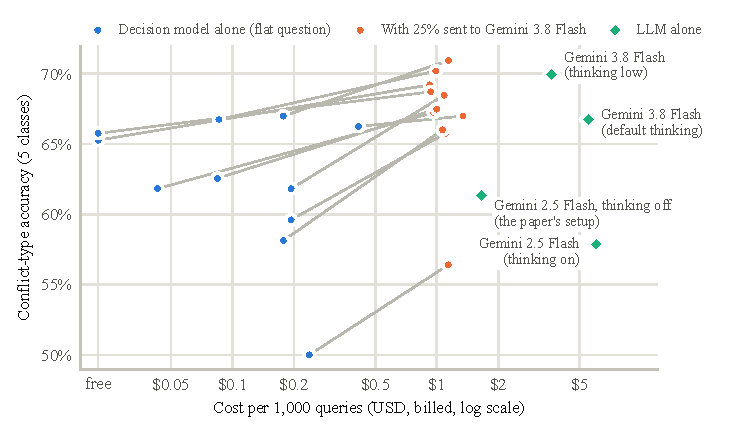
\includegraphics[width=0.78\textwidth]{figures/cascade_cost_accuracy.pdf}
\caption{Accuracy against cost (log scale) on the test split. Curves: \jev answers first and the least confident
fraction of queries goes to Gemini~3.8 Flash; dots mark 25\% and 50\% escalated (at 25\% the two curves nearly
coincide). Diamonds: LLMs alone with the paper's prompt.}
\label{fig:cascade}
\end{figure*}

\subsection{Diagnostics}
\label{sec:diagnostics}

We specified three hypotheses and their tests before running them; Tables~\ref{tab:diagnostics}
and~\ref{tab:plant} give the results. An identical rerun sets the noise floor: no system is deterministic, and
\jev changes its predicted type on \diagjfrerunflip\% of queries with nothing changed (Gemini~3.8 Flash:
\diaggmrerunflip\%).

\begin{table*}[t]
\centering\footnotesize\setlength{\tabcolsep}{4pt}
\fitwidth{\begin{tabular}{lccccccccc}
\toprule
 & \multicolumn{3}{c}{Jev flat} & \multicolumn{3}{c}{Jev tree v2$^\dagger$} & \multicolumn{3}{c}{Gemini 3.8} \\
\cmidrule(lr){2-4}\cmidrule(lr){5-7}\cmidrule(lr){8-10}
Perturbation & $\Delta$Acc ($p$) & Flip & Outd. & $\Delta$Acc ($p$) & Flip & Outd. & $\Delta$Acc ($p$) & Flip & Outd. \\
\midrule
Rerun & $-$0.5 (0.69) & 2.0 & 74.5 & $-$0.2 (1.00) & 2.5 & 20.0 & +1.2 (0.27) & 3.4 & 72.7 \\
No dates & $-$1.0 (0.34) & 3.0 & 74.5 & +0.0 (1.00) & 3.4 & 20.0 & $-$0.7 (0.51) & 2.7 & 67.3 \\
Recency in code & +0.2 (1.00) & 3.4 & 76.4 & +0.2 (1.00) & 3.7 & 21.8 & $-$0.7 (0.65) & 5.7 & 72.7 \\
Shuffle, seed 1 & +1.5 (0.38) & 11.1 & 72.7 & $-$1.5 (0.33) & 9.9 & 18.2 & $-$0.5 (0.85) & 8.4 & 74.5 \\
Shuffle, seed 2 & +0.2 (1.00) & 12.1 & 67.3 & $-$2.2 (0.11) & 8.4 & 18.2 & $-$2.7 (0.09) & 10.3 & 70.9 \\
\midrule
Original Outd.\ recall & \multicolumn{3}{c}{72.7} & \multicolumn{3}{c}{20.0} & \multicolumn{3}{c}{69.1} \\
\bottomrule
\end{tabular}}
\caption{Diagnostics on the test split. Each perturbed run is compared with the same system's original run. $\Delta$Acc: accuracy change in points (exact McNemar $p$). Flip: share of queries whose predicted type changed (\%). Outd.: recall (\%) on the 55 \emph{Outdated} queries after the perturbation. The identical rerun is the noise floor. $^\dagger$Revised on development data.}
\label{tab:diagnostics}
\end{table*}


\paragraph{Dates do not matter.} \jev's documentation lists ordering dates as a known weakness
\citep{typesafe2026jagged}, and we expected it to explain errors on \emph{Outdated}. It does not. Removing every
date changes no system's accuracy beyond the noise floor (\jev: \diagjfnodatesdiff points, $p\diagjfnodatesp$;
Gemini: \diaggmnodatesdiff, $p\diaggmnodatesp$), and neither does adding each result's recency rank computed in
code. \jev's recall on \emph{Outdated} is \diagjforigrec\% originally, \diagjfnodatesrec\% without dates and
\diagjfdatesincoderec\% with code-computed recency, at or above Gemini's in every condition. The systems recognise
outdated sources from their content (phrases such as ``former'' or ``as of'', and conflicting values), not from
publication dates. The weak \emph{Outdated} score of tree v2 comes from its question design, not from dates.

\paragraph{Order sensitivity is real but not specific to \jev.} Shuffling the results changes \jev's predicted type
on \diagjfshuffleflip\% of queries [\diagjfshufflelo, \diagjfshufflehi] over both seeds, well above its
\diagjfrerunflip\% noise floor; Gemini~3.8 Flash flips on \diaggmshuffleflip\%
[\diaggmshufflelo, \diaggmshufflehi]. On the same shuffles the two do not differ ($p\diagflipjevvsgonep$ and $p\diagflipjevvsgtwop$). Accuracy moves by at most a few points in either direction.

\begin{table*}[t]
\centering\small
\fitwidth{\begin{tabular}{lccccc}
\toprule
System & Hit & False al. & Youden & Any conflict & AUROC \\
\midrule
Jev 1.13, flat & 66.7 & 17.7 & +0.490 & 85.4 / 41.7 & 0.81 \\
Jev 1.13, tree v2$^\dagger$ & 19.8 & 2.1 & +0.177 & 67.7 / 25.0 & 0.70 \\
Gemini 3.8 Flash (low) & 52.1 & 3.1 & +0.490 & 71.9 / 25.0 & -- \\
\bottomrule
\end{tabular}}
\caption{One planted false source in 96 \emph{No conflict} test queries (expected label: \emph{Misinformation}). Hit: planted copy labelled Misinformation. False al.: clean copy of the same query labelled Misinformation. Youden = hit $-$ false alarm. Any conflict: planted / clean copy not labelled No conflict. AUROC: P(Misinformation) separating planted from clean copies. $^\dagger$Revised on development data.}
\label{tab:plant}
\end{table*}


\paragraph{A planted false source is noticed as well as by the LLM.} \conflicts has too few \emph{Misinformation}
queries to evaluate. We construct them: in \nplant \emph{No conflict} test queries whose gold answer appears in some
result, we rewrite one such result so that it states a plausible wrong answer, produced by a third model
(GPT-4.1-mini) so that neither classifier judges its own text. The expected label becomes \emph{Misinformation}.
Flat \jev labels \plantjfhit\% of planted queries as misinformation against \plantgmhit\% for Gemini~3.8 Flash
($p\planthitp$), but it also does so for \plantjffa\% of the clean versions of the same queries against
\plantgmfa\% ($p\plantfap$). Net of false alarms the two are identical (Youden \plantjfyouden each; difference
\plantyoudendiff [\plantyoudenlo, \plantyoudenhi]). \jev's misinformation probability separates planted from clean
versions with AUROC \plantjfauroc, so a threshold can trade detections for fewer false alarms. Tree v2, whose
misinformation rule was chosen on a development split with a single misinformation query, detects only
\plantjthit\%.

\subsection{Robustness across versions and decision models}
\label{sec:robustness}

\paragraph{\jev 1.14.} The newer version behaves like 1.13 (Table~\ref{tab:main}): \onefouracc\% with the flat
question (\onefourvsonethreediff points, $p\onefourvsonethreep$) and \onefourtreeacc\% with tree v2
($p\onefourtreevsonethreep$), still tied with Gemini~2.5 Flash ($p\onefourvstwofivep$), with the same failure
of tree v1 and the same cascade behaviour (tree v2 at 50\%: \onefourcascfiftyacc\%, $p\onefourcascfiftyp$ against
the LLM alone).

\begin{table*}[t]
\centering\small\setlength{\tabcolsep}{5pt}
\fitwidth{\begin{tabular}{lccccccc}
\toprule
Decision model & Flat & Tree v2 & ECE & \$ / 1k & Lat.\ (s) & $\Delta$ Jev ($p$) & $\Delta$ Gemini 3.8 ($p$) \\
\midrule
Jev 1.13 & 61.8 & 63.5 & 0.103 & 0.19 & 0.26 & -- & $-$8.1 ({<}0.001) \\
Perplexity v1.2 & 66.7 & 69.0 & 0.061 & 0.09 & 0.42 & +4.9 (0.03) & $-$3.2 (0.14) \\
GPT-6-luna & 66.3 & 50.0 & 0.059 & 0.41 & 0.35 & +4.4 (0.11) & $-$3.7 (0.13) \\
Liquid d1 & 62.6 & 58.4 & 0.075 & 0.08 & 0.41 & +0.7 (0.83) & $-$7.4 (0.002) \\
Microsoft d-1 & 58.1 & 57.4 & 0.188 & 0.18 & 0.45 & $-$3.7 (0.13) & $-$11.8 ({<}0.001) \\
\bottomrule
\end{tabular}}
\caption{Jev against the other decision models available through the same gateway, with Jev's frozen questions and inputs, nothing tuned per model (test split). Flat, Tree v2: accuracy (\%). ECE and latency for the flat question. $\Delta$: accuracy difference of the flat question from Jev and from Gemini~3.8 Flash in points, with exact McNemar $p$. Models: Perplexity decider v1.2, OpenAI GPT-6-luna decisions, Liquid d1, Microsoft decision-1. Gemini 3.8 Flash (thinking low) scores 70.0\% at \$3.65 per 1k queries.}
\label{tab:decision_models}
\end{table*}


\paragraph{Other decision models.} Table~\ref{tab:decision_models} places \jev among the decision models
available through the same gateway. \jev is mid-pack in accuracy and the fastest. Perplexity's decider is the most
accurate: \pplxflatacc\% with the flat question, \pplxvsjevdiffabs points above \jev ($p\pplxvsjevp$), and
\pplxtreeacc\% with tree v2, statistically tied with Gemini~3.8 Flash ($p\pplxtreevsgp$). As a cascade first
stage it reaches \cascpplxtfacc\% at \cascpplxtfcost\% of the LLM's cost at $f=25\%$. Not every decision model's
confidence is useful for escalation: GPT-6-luna's confidence barely ranks its errors (AUROC \lunaauroc), and its
25\% cascade is no better than random escalation (\lunacasctf\% vs.\ \lunacasctfrand\%).

\section{Discussion}
\label{sec:discussion}

\paragraph{What decision models offer as conflict classifiers.} Conflict typing sits on the critical path of every
search-augmented answer, so its latency and cost add to every request. Most hosted decision models classify a query
with about ten retrieved pages in under half a second, for at most \$\dmcostmax per thousand queries, with the accuracy of the LLM used in the original study. When the accuracy of a
current LLM is required, a decision model's confidence is usually good enough to route only its uncertain queries to
the LLM, which recovers most of the gap at a quarter to a third of the LLM's cost. End to end, the cheaper types cost
no measurable answer quality (\S\ref{sec:endtoend}). 

\paragraph{Choosing among decision models.} The class is not uniform. Accuracy spans \dmaccmin--\dmaccmax\%, and the
model at the bottom is significantly worse than the paper's LLM. Two properties that matter in deployment vary
independently of accuracy: calibration (ECE \eceminimum--\ecemaximum) and how well confidence ranks errors, which
decides whether a cascade helps at all. One of the most accurate models has confidence that is no better than random for
escalation. A model for this task should therefore be chosen on all three, measured on the deployment's own data,
not on accuracy alone.

\paragraph{How to ask.} The direct choice question was the reliable format for every model. The yes/no
decomposition looked natural but failed for all of them; the repaired tree encodes choices fitted to one model on a
small development split and did not help any other. For a new decision model we would start from the flat
question.

\paragraph{What the diagnostics change.} Dates turned out not to matter: outdated sources are recognised
from their content. Sensitivity to source order is real but differs so much between models that it has to be
measured for each one. A single false source is the subtle case, visible in the probabilities but rarely in the
top label. With
\nmisitest natural \emph{Misinformation} test queries, that type is the one a deployment would most need to
calibrate on its own data.

\paragraph{Limitations.}
(i) \conflicts is small: with \ntest test queries, differences under about five points are not significant, and the
cascades can be shown close to, but not formally equivalent to, the LLM. (ii) The label distribution reflects how the
queries were selected, not real search traffic, and the dataset has only five natural \emph{Misinformation}
queries; our planted variant tests one kind of misinformation (an entity or value substituted in a single source).
(iii) The census covers the decision models one gateway served on one day. Hosted models change without notice:
several identifiers are unversioned, two models were free during our runs, and our rerun of Gemini~2.5 Flash scores
below the published figure. Providers
do not disclose model sizes or training data, so we cannot explain the differences between models. (iv) The end-to-end test uses one generator and LLM judges, validated on \nvalid answers, that do not see the
search results; as in the original study, the primary judge is the generator's own model, which may favour its
answers \citep{panickssery2024llm}. The size of the gain from predicted types depends on the judge, and we do not
measure factual grounding, the third metric of \citet{cattan2025dragged}. (v) Not every system is deterministic: identical requests changed
up to \rerunflipmax\% of a decision model's predictions, and \diaggmrerunflip\% of Gemini~3.8 Flash's.

\section{Conclusion}
\label{sec:conclusion}

We tested every typed decision model hosted on one gateway as a classifier of knowledge-conflict types, using
the benchmark authors' protocol and the same inputs as the LLMs. Most match the LLM of the original study. They do
so at a small fraction of its cost and latency. They trail the
current LLM, but for most of them a confidence-gated cascade recovers that gap at a quarter to a third of the LLM's
cost, and given to a generator, their types yield answers that follow the expected behaviour as often as the LLM's.
 Future work should measure the gain from predicted types with judges that see the
sources, and test whether a decision model's probabilities can steer a generator between expected behaviours when
the type is uncertain.

\section*{Ethics and Broader Impact}

The planted-misinformation variant rewrites one retrieved page per query to state a wrong answer. It uses public data and factual substitutions on
non-sensitive questions, and is released with clear labels. All queries in \conflicts are safe by construction \citep{cattan2025dragged}. Cheap conflict
classification could be misused to suppress minority viewpoints; the expected behaviour for \emph{Conflicting
opinions} is to present all of them.


\bibliography{refs}
\bibliographystyle{acl_natbib}

\appendix
\section{Prompts and Questions}
\label{app:prompts}

\paragraph{LLM prompt.} The conflict-type prompt of \citet{cattan2025dragged}, copied from the paper's source with
only the \LaTeX{} bold markers removed. \texttt{\{search\_results\}} is filled with the numbered results.

\lstinputlisting{generated/paper_prompt.txt}

\paragraph{\jev, flat.} One choice question. Its instruction is the first paragraph of the prompt above; its options
are the five category definitions with their examples, word for word.

\lstinputlisting{generated/flat_question.txt}

\paragraph{\jev, tree.} Five yes/no questions asked in one request over the same state.

\lstinputlisting{generated/tree_questions.txt}

\paragraph{Planted wrong answers.} Prompt sent to GPT-4.1-mini (temperature 0) to obtain a plausible wrong answer
for each \emph{No conflict} query whose gold answer appears in a result. The answer is then replaced, as whole words
and case-insensitively, in the title, snippet and text of one such result chosen with a fixed seed. Queries whose
gold answer is \emph{yes} or \emph{no} are excluded.

\lstinputlisting{generated/wrong_answer_prompt.txt}

\section{Protocol Record}
\label{app:protocol}

The development/test split, the prompt and question texts and the combination rules were frozen with recorded file
hashes before any test-set call. Changes after that point were limited to the following, each logged with its reason
before results were computed: (1) Gemini~2.5 Flash with thinking added as a sensitivity check; (2) the answer parser
made lenient for category statements outside the requested JSON, applied to stored answers without new calls (no
strictly formatted answer changed); (3) Gemini~3.8 Flash added at two thinking levels; (4) the cascade, its
operating points and its controls; (5) the diagnostics, with one amendment before any planted run: whole-word
matching and the exclusion of yes/no answers, after substring matching was found to alter unrelated numbers;
(6) \jev 1.14 and the four other decision models, run with \jev's frozen questions. All runs were reported. Code,
splits, prompts, cached responses and per-query outputs are released.


\end{document}
